%%%%%%%%%%%%%%%%%%%%%%%%%%%%%%%%%%%%%%%%%%%%%%%%%%%%%%%%%%%%%%%%%%%%%%%%
%
% Pangloss: Testing the reconstruction paper
%
%%%%%%%%%%%%%%%%%%%%%%%%%%%%%%%%%%%%%%%%%%%%%%%%%%%%%%%%%%%%%%%%%%%%%%%%

\documentclass[useAMS,usenatbib]{mn2e}
%% letterpaper
%% a4paper

% \voffset=-0.8in

% Packages:
\input psfig.sty
\usepackage{xspace}
\usepackage{graphicx}
\usepackage{amssymb}
\usepackage{amsmath}

% Macros:
% JOURNALS
\newcommand{\apj}{ApJ}
\newcommand{\apjl}{ApJL}
\newcommand{\apjs}{ApJS}
\newcommand{\mnras}{MNRAS}
\newcommand{\apss}{Ap \& SS}
\newcommand{\aap}{A\&A}
\newcommand{\aj}{AJ}
\newcommand{\prd}{Phys. Rev. D}
\newcommand{\nat}{Nature}
\newcommand{\araa}{ARA\&A}
\newcommand{\jgr}{J. Geophys. Res.}
\newcommand{\pasp}{PASP}

% MISC
\newcommand{\etal}{et~al.~}
\def\spose#1{\hbox  to 0pt{#1\hss}}  
\newcommand{\lta}{\mathrel{\spose{\lower 3pt\hbox{$\sim$}}\raise  2.0pt\hbox{$<$}}}
\newcommand{\gta}{\mathrel{\spose{\lower  3pt\hbox{$\sim$}}\raise 2.0pt\hbox{$>$}}}
\newcommand{\eg}{{\it e.g.\ }}
\newcommand{\ie}{{\it i.e.\ }}
\newcommand{\be}{\begin{equation}}
\newcommand{\ee}{\end{equation}}
\newcommand{\dee}{\, \mathrm{d} \!}
\newcommand{\bea}{\begin{eqnarray}}
\newcommand{\eea}{\end{eqnarray}}


% CROSS-REFERENCING
\def\Sref#1{Section~\ref{#1}\xspace}
\def\Fref#1{Figure~\ref{#1}\xspace}
\def\Tref#1{Table~\ref{#1}\xspace}
\def\Eref#1{Equation~\ref{#1}\xspace}
\def\Eqref#1{Eq.~(\ref{#1})\xspace}
\def\Aref#1{Appendix~\ref{#1}\xspace}

% UNITS
\newcommand{\kms}{\ifmmode  \,\rm km\,s^{-1} \else $\,\rm km\,s^{-1}  $ \fi }
\newcommand{\kpc}{\ifmmode  {\rm kpc}  \else ${\rm  kpc}$ \fi  }  
\newcommand{\pc}{\ifmmode  {\rm pc}  \else ${\rm pc}$ \fi  }  
\newcommand{\Msun}{\ifmmode {\rm M_{\odot}} \else ${\rm M_{\odot}}$ \fi} 
\newcommand{\Zsun}{\ifmmode {\rm Z_{\odot}} \else ${\rm Z_{\odot}}$ \fi} 
\newcommand{\yr}{\ifmmode yr^{-1} \else $yr^{-1}$ \fi} 
\newcommand{\hMsun}{\ifmmode h^{-1}\,\rm M_{\odot} \else $h^{-1}\,\rm M_{\odot}$ \fi}

% COSMOLOGY
\newcommand{\LCDM}{$\Lambda{\rm CDM}$}
\newcommand{\MS}{Millennium Simulation\xspace}

% LENSING
\def\zd{z_{\rm d}}
\def\zs{z_{\rm s}}
\def\Dd{D_{\rm d}}
\def\Ds{D_{\rm s}}

\def\Dt{D_{\Delta t}}

\def\Dds{D_{\rm ds}}
\def\Sigmacrit{\Sigma_{\rm crit}}
\def\REin{R_{\rm Ein}}
\def\MEin{M_{\rm Ein}}
\def\xkappa{\kappa_{\rm ext}}
\def\kappax{\kappa_{\rm ext}}
\def\kappaxtrue{\kappax^{\rm true}}
\def\kappah{\kappa_{\rm h}}
\def\kappav{\kappa_{\rm void}}
\def\kapparay{\kappa_{\rm raytrace}}
\def\kapparec{\kappa_{\rm reconstruction}}
\def\kappatrue{\kappa_{\rm true}}
\def\kappahalo{\kappa_{\rm halo}}
\def\Pkh{{\rm P}(\kappa_{\rm h})}
\def\Pk{{\rm P}(\kappa)}
\def\kappah{\kappa_{\rm h}}
\def\kappahk{\kappa_{{\rm h},k}}
\def\gammah{\gamma_{\rm h}}
\def\gammax{\gamma_{\rm ext}}


\def\sumkappah{\sum_{\rm halos} \kappa_{\rm halo}}
\def\sigt{\tilde{\sigma}}


% HALO MODEL PARAMETERS
\def\Mstar{M^{*}}
\def\logMstar{\log_{10}\left(\Mstar/\Msun\right)}
\def\Mstarobs{\Mstar_{\rm obs}}
\def\Mstarobsk{\Mstar_{{\rm obs},k}}
\def\Mhalo{M_{200}}
\def\Mh{M_{200}}
\def\logMhalo{\log_{10}\left(\Mhalo/\Msun\right)}
\def\Mhalok{M_{200,k}}
\def\Rhalo{R_{200}}
\def\chalo{c_{200}}

% SOFTWARE/HARDWARE
\def\SExtractor{{\sc SExtractor}\xspace}
\def\hst{{\it HST}\xspace}
\def\acs{\hst/ACS\xspace}
\def\galfit{{\sc galfit}\xspace}
\def\idl{{\sc idl}\xspace}
\def\python{{\sc python}\xspace}
\def\Pangloss{{\sc Pangloss}\xspace}

% TABLES:
\newcommand\nodata{ ~$\cdots$~ }%

% PROBABILITY THEORY
% % Phil:
% \def\pr{{\rm Pr}}
% \def\data{{\mathbf{d}}}
% \def\datap{{\mathbf{d}^{\rm p}}}
% \def\datai{d_i}
% \def\datapi{d^{\rm p}_i}
% Tom:
\def\pr{{\rm P}}
\def\data{{\mathcal{D}}}
\def\datap{{\data}^{\rm p}}
\def\datai{{\data}_i}
\def\datapi{{\data}^{\rm p}_i}

\def\sigi{\sigma_{\rm intrinsic}}

% COMMENTING
\usepackage[usenames]{color}
\newcommand{\phil}[1]{\textcolor{blue}{\bf #1}}
\newcommand{\matt}[1]{\textcolor{orange}{\bf #1}}
\newcommand{\tom}[1]{\textcolor{OliveGreen}{\bf #1}}
\newcommand{\todo}[2]{\textcolor{red}{\bf TO DO (#1): #2}}
\newcommand{\flag}[1]{\textcolor{red}{\bf #1}}
\newcommand{\comment}[1]{}
\newcommand{\comments}[1]{}
\newcommand{\notes}[1]{\textcolor{cyan}{#1}}
\newcommand{\new}[1]{\textcolor{magenta}{#1}}


% SPELLING:
\def\devided{divided\xspace}
\def\truely{truly\xspace}
\def\infered{inferred\xspace}
\def\correspends{corresponds\xspace}
\def\independant{independent\xspace}
\def\dependant{dependent\xspace}
\def\proceedure{procedure\xspace}
\def\propogate{propagate\xspace}
\def\propogates{propagates\xspace}
\def\succesful{successful\xspace}


\def\ioa{Institute of Astronomy, University of Cambridge,
  Madingley Rd, Cambridge, CB3 0HA, UK}
\def\oxford{Dept.\ of Physics, University of Oxford, 
  Keble Road, Oxford, OX1 3RH, UK}
\def\kipac{Kavli Institute for Particle Astrophysics and Cosmology, 
 Stanford University, 452 Lomita Mall, Stanford, CA 94035, USA}
\def\ucsb{Dept.\ of Physics, University of California, 
  Santa Barbara, CA 93106, USA}
\def\davis{Dept.\ of Physics, U.C.~Davis, Davis, CA 95616, USA}
\def\kapteyn{Kapteyn Astronomical Institute, University of Groningen, 
  P.O.Box 800, 9700 AV Groningen, The Netherlands}
\def\asiaa{5}{Institute of Astronomy and Astrophysics, Academia Sinica, P.O.~Box 23-141, Taipei 10617, Taiwan}

\def\collettemail{\tt t.collett@ast.cam.ac.uk}

\def\packard{Packard Research Fellow}


%%%%%%%%%%%%%%%%%%%%%%%%%%%%%%%%%%%%%%%%%%%%%%%%%%%%%%%%%%%%%%%%%%%%%%%%%%%%%%

\title[Line of Sight Mass Reconstruction]
{Inferring Lensing Mass in the Universe \\
from Photometric Catalog Data}
    
\author[Collett \etal]{%
  Thomas~E.~Collett$^{1}$\thanks{\collettemail},
  Philip~J.~Marshall$^{2}$,
  Matthew~W.~Auger$^{1}$,
  Stefan~Hilbert$^{3}$,
\newauthor{%
  Sherry~H.~Suyu$^{4}$,
  Zachary~Greene$^{4}$,
  Tommaso~Treu$^{4}$\thanks{\packard},
  Christopher~D.~Fassnacht$^{5}$,}
\newauthor{%
  L\`eon~V.~E.~Koopmans$^{6}$,
  Roger~D.~Blandford$^{3}$} 
  \medskip\\
  $^1$\ioa\\
  $^2$\oxford\\
  $^3$\kipac\\
  $^4$\ucsb\\
  $^5$\davis\\
  $^6$\kapteyn
}

%%%%%%%%%%%%%%%%%%%%%%%%%%%%%%%%%%%%%%%%%%%%%%%%%%%%%%%%%%%%%%%%%%%%%%%%%%%%%%

\begin{document}
             
\date{to be submitted to MNRAS}
\pagerange{\pageref{firstpage}--\pageref{lastpage}}\pubyear{2012}

\maketitle           

\label{firstpage}

%%%%%%%%%%%%%%%%%%%%%%%%%%%%%%%%%%%%%%%%%%%%%%%%%%%%%%%%%%%%%%%%%%%%%%%%%%%%%%

\begin{abstract} 

Strong gravitational lenses can provide high precision cosmological distance
measurements; one of the most important sources of systematic error in these
estimates is the additional mass along the line of sight to the source. Weak
lensing by galaxies and groups in this beam can contribute an ``external
convergence'' $\xkappa$ that dominates the  uncertainty in the inferred
distances; likewise, it may also contaminate estimates of the luminosity of
objects at high redshift (such as reionisation-era proto-galaxies, and type Ia
supernovae standard candles).  We characterise this uncertainty by marginalising
over a probability density function for $\xkappa$: here, we investigate the use
of a simple halo model to estimate $\Pr(\xkappa)$ given noisy estimates of the
photometric redshift and stellar mass of galaxies observed in optical imaging
surveys of the field in question. We use mock catalogs from the Millenium
Simulation and compare our reconstructed $\Pr(\xkappa)$ to ray-traced $\kappa$ values,
we find that our model produces an unbiased estimator of $\kappax$,
For each lightcone the individual $\Pr(\xkappa)$ from this reconstruction process are
typically 1.8 times narrower than the global distribution of $\xkappa$ given perfect knowledge 
of the halo mass and redshift. After incorporating uncertainties on redshift and halo and stellar masses
we typically find that the reconstruction yields an improvement factor of 1.5. For each line of sight the
 $\Pr(\xkappa)$ can be formed before the investment of light-curve monitoring. By following up only the 
most costrained lines of sight a factor of 2 improvement over the global $\pr(\kappax)$ should be 
achievable.
\end{abstract}

% Full list of options at http://www.journals.uchicago.edu/ApJ/instruct.key.html

\begin{keywords}
  gravitational lensing   --
  methods: statistical    --
  galaxies: halos         --
  gaaxies: mass function  --
  cosmology: observations
\end{keywords}

\setcounter{footnote}{1}

%%%%%%%%%%%%%%%%%%%%%%%%%%%%%%%%%%%%%%%%%%%%%%%%%%%%%%%%%%%%%%%%%%%%%%%%%%%%%%

\section{Introduction}

Averaged over large areas of sky, the weak gravitational lensing effect can be
used to constrain the statistical properties of the matter density in the
Universe: every distant object we observe has had its shape distorted, and size
and total brightness magnified (or demagnified) by a compound lens constructed
from all the mass distributed between us and it.

This fact makes weak gravitational lensing a potentially important source of
systematic error for any estimate of luminosity or distance, an issue
raised for \eg 
type Ia supernovae by \citet[][]{Holz+Wald1998,Linder+Holz2004}, for
gamma ray bursts by \citet[][]{Oguri+Takahashi2006,Wang+Dai2011}, 
and for high redshift galaxies by \citet{BradacEtal2009}, among others. 
Along lines of sight containing strong gravitational lenses,
the effect has been found to be
particularly important, with foreground and background structures
having a significant effect on the inferred lensing cross-section
\citep[\eg][]{WongEtal2012} and distance ratios \citep[][]{DalalEtal2005}.
In time delay lens cosmography,
\citet{SuyuEtal2010} found that  the lensing effect of mass structures along the
(unusually over-dense)  line of sight to the quadruply-imaged radio source
B1608$+$656, the so-called ``external convergence,'' was the dominant source
of uncertainty in their 6\% measurement of Hubble's constant. 

How can we correct for this weak lensing error, and make
accurate measurements through the Universe? When inferring global quantities
(such as the cosmological parameters), averaging the results from a large
number of independent objects will tend to reduce the error, as the
ensemble-averaged convergence approaches zero for an unbiased sample
\citep[\eg][]{Linder+Holz2004}. If the sample is biased, however, some
residual systematic error will remain while the statistical uncertainty
decreases -- and this will be the case for any sample selected by the
brightness of the lensed object, or any other quantity that depends on
$\xkappa$. The latter class includes time delay lenses, which could be
either detected or selected 
based on their image separations, magnifications or quadruple image
configurations, all of which either increase or become more likely with
increasing $\kappa$. Large
samples of lenses are expected to be discovered in the next decade in
ground-based optical imaging surveys \citep{Oguri+Marshall2010} -- but these
samples will be image separation-limited, due to the surveys' relatively poor
($\sim 1$~arcsec) image quality. Some of the current sample of known time
delay lenses were detected in surveys like this: we might expect them to be
somewhat biased towards high values of $\xkappa$.

There are two broad approaches one could take at this point. First, one could
seek to characterise the lensed objects' selection function, and use this
understanding to derive a suitable correction to cosmological parameters
inferred assuming no $\xkappa$ at all. As pointed out by  \citet[][among
others]{Oguri+Takahashi2006}, to do this one would need  information about the
unlensed population of objects, and the population of lenses, and how the
objects were detected -- or to infer these hierarchically during the analysis.
Alternatively, one could simply accept all lenses provided, regardless of
their selection, and try to use any additional information that is available
to estimate the external convergence in each system on a case by case basis,
and hence optimize their joint analysis to produce a better-constrained result
\citep[as suggested by][]{Keeton+Zabludoff2004}. In this work we follow this
second approach, and use measurements of the positions, magnitude and colours
of galaxies close to lens lines of sight to try to infer the
external convergence at the lens position. 

Attempts to date at reconstructing the local and  line of sight mass
distribution in strong lens fields (what \citeauthor{WongEtal2011} call ``the
full environment'') have focused on photometric and  spectroscopic surveys to
detect galaxy groups and ascertain galaxies' membership,  and on understanding
the external shear apparently required by the strong lens models. Surveys by
\citet{Fassnacht+Lubin2002,AugerEtal2007,WilliamsEtal2006,MomchevaEtal2006}
all found groups of galaxies both hosting and lying  along the line of sight
to known gravitational lenses. Initial estimates of the effect of these
structures suggested the importance of assigning mass to both galaxy and group
halos, and to allowing for significant uncertainty in the centroids of group
halos. The probability density function (PDF) for the external convergence for
that lens, $\Pr(\xkappa)$, is the target for any reconstruction analysis, and
is the key quantity for any ensemble analysis, since by marginalising over it
we can correctly propagate the uncertainties due to weak lensing. Coming
closest to estimating this quantity from survey data, \citet{WongEtal2011} ran
Monte Carlo reconstructions of the mass in nine lens fields based on
\citeauthor{WilliamsEtal2006} and \citeauthor{MomchevaEtal2006}'s
photometric and spectroscopic measurements of galaxies close to the line of
sight, and compared the resulting predicted shear distributions with the
external shear demanded by the strong lens model. Their simulations show most
of the shear being generated by bright galaxies within 2~arcminutes of the
lens, and that both line of sight structures and the group of galaxies in each
lens plane contribute significant proportions of the shear. They find
significant discrepancies between the lens model shear and the Monte Carlo
predictions, and are unable to distinguish between the environment modelling
and the strong lens modelling as the cause of these discrepancies.

These observational investigations have provided very useful insight into the
problem.  Coming from a more theoretical direction, large numerical
simulations have been used to predict, from first principles, the distribution
of likely external shears and convergences along strong lens lines of sight. 
\citet{Holder+Schechter2003} and \citet{Dalal+Watson2004} carried out
ray-tracing calculations in N-body simulations to estimate the  distribution
of external shear values.  \citet{HilbertEtal2009} performed similar ray-tracing
experiments through the Millenium Simulation \citep{SpringelEtal2005},
generating a predicted $\xkappa$ at every position in a simulated sky. The
first step towards using this excellent calibration resource was taken by
\citet{SuyuEtal2010}, who selected Millenium Simulation lines of sight that a)
were found to contain a strong lens and b) had comparable apparent galaxy
overdensity in a 45 arcsec radius aperture down to $i < 24$. This overdensity
could be compared to the overdensity of the B1608$+$656 line of sight
\citep{FassnachtEtal2011}, and hence an estimate of  $\Pr(\xkappa)$ could be
made. 

In this paper, we bring these observational and theoretical approaches
together and  use numerical simulations to {\it test and calibrate} a
reconstruction of the  external convergence. Ray-tracing through the
simulations gives a ``truth'' that we can attempt to recover.  In this paper
we use the Millenium Simulation mock galaxy catalogs and ray-traced lensing
effects to test the accuracy of line of sight mass reconstructions.
Probabilistically ssigning mass and redshift to every observed galaxy in the
field around a time delay lens, we generate Monte Carlo sample line of sight
mass distributions, and estimate the external convergence due to each one.
This gives us a $\Pr(\xkappa)$ that can be propagated into further joint
inferences. We focus on time delay lens cosmography, and quantify our results
in terms of the uncertainty on the mean time delay distance to a test sample
of $N$ lenses (where for clarity each lens has the same deflector and source
redshift, and the same lens model and time delay uncertainty).

We aim to answer the following questions:
\begin{itemize}
\item Faint galaxies and other dark structures will not appear in a photometric
object catalog, but they will contribute convergence at some level. How much of
the total external convergence in a time delay lens system comes from visible
galaxies? How does this change as a function of magnitude cut? 
\item Can the true (ray-traced) convergence be recovered by halo model
reconstruction? What scatter and residual bias are induced in the ensemble 
distance estimate? Which aspects of the model dominate these uncertainties? 
\item When faced with a newly-detected lens, surrounded by galaxies on the sky,
we have some choices to make when planning follow-up observations.
Which are the most important galaxies, with regard to the external convergence
produced? Can nearby groups and clusters be straightforwardly accounted for? If
lenses with such massive structures nearby are discarded, what impact does that
have on the distance accuracy?
\end{itemize}

This paper is organized as follows. In~\Sref{sec:theory} we review the relevant
gravitational lensing theory, before introducing our simple reconstruction 
model in \Sref{sec:model}.  We then test this model in two phases: first, in
\Sref{sec:knownMh+z}, with known redshift and halo mass for every galaxy in a
lens field, in order to quantify the irreducible uncertainty due to unseen mass,
and second, in \Sref{sec:obsMstar+z}, with realistic observational uncertainties
on the field galaxies' stellar masses and redshifts. \comments{We then propagate all these
uncertainties through to the time delay distance in a toy sample of 100 lenses,
in \Sref{sec:distances}.} We discuss our results in \Sref{sec:discuss} before
concluding in \Sref{sec:conclude}.

Throughout this paper magnitudes are given in the AB system and
we adopt the Millenium Simulation's ``concordance'' parameters for our reference cosmology, \ie
$h=0.73$, $\Omega_m=0.25$ and $\Omega_\Lambda=0.75$, where the symbols indicate
the Hubble Constant in units of 100 km s$^{-1}$ Mpc$^{-1}$ and the matter and
dark energy density of the Universe in units of the critical density
.%\citep[e.g.\ ][]{KomEtal09}.


%%%%%%%%%%%%%%%%%%%%%%%%%%%%%%%%%%%%%%%%%%%%%%%%%%%%%%%%%%%%%%%%%%%%%%%%%%%%%%

\section{Theoretical Background}
\label{sec:theory}

%Time delay distances, and the mass sheet degeneracy - how kappa is degenerate in
%strong lens models (and magnifications).


Convergence, or Ricci focusing, occurs when a gravitational lens focuses the rays in a raybundle.
This focussing can cause distant objects to appear brighter, and larger than they would if the lens
 were removed.
The convergence from an isolated mass sheet is the ratio of the projected surface mass density
($\Sigma(D_{\mathrm{od}}\bmath{\theta})$) devided by the critical surface mass density at the redshift of the mass sheet ($\Sigma_{\rm cr}$),
\be
\kappa(\bmath{\theta})= \frac {\Sigma(D_{\mathrm{od}}\bmath{\theta})}{\Sigma_{\rm cr}(z)}
\ee
where 
\be \label{eq:sigcrit} 
\Sigma_{\rm cr}(z) \equiv \frac{c^2 D_{\rm os}}{4 \pi G D_{\rm od} D_{\rm ds}}.
\ee
and the D's are the angular diameter distances between the objects refered to in the subscripts: o is the observer, d is the deflector and s is the source. If the surface mass density of the sheet exceeds $\Sigma_{\rm cr}$, multiple images of the source can
occur, otherwise only one image will be observed, although that image will still be perturbed
relative to the unlensed case.

Strong lensing occurs when a massive object and background source are almost perfectly
aligned along a line of sight. The light from the background source is deflected by the
lens galaxy; this deflection allows multiple images of the background source to form
at stationary points of the time delay function. For an isolated lens, the time delay
function can be calculated from
\be \label{eq:T} 
\Delta t(\bmath{\theta},\bmath{\beta}) = \frac {1}{c} \frac{D_{\rm od} D_{\rm os}}{D_{\rm ds}} (1+z_{\rm d})\, \phi(\bmath{\theta},\bmath{\beta}),
\ee
where $\bmath{\theta}$ is the observed source position, $\bmath{\beta}$ is the 
unlensed source position, $z_{\rm d}$ is the redshift of the lens, $\phi(\bmath{\theta},\bmath{\beta})$ is
the Fermat potential. The Fermat potential is given by
\be \label{eq:FP}
\phi(\bmath{\theta},\bmath{\beta})\equiv \left[\frac{(\bmath{\theta}-\bmath{\beta})^2}{2}-\psi(\bmath{\theta}) \right], 
\ee
where $\psi(\bmath{\theta})$ is the lens potential, derived from the projected dimensionless
surface mass density, $\kappa(\bmath{\theta})$, by 
\be \label{eq:psikappa}
\kappa(\bmath{\theta})=\frac{1}{2}\nabla^2\psi(\bmath{\theta}).
\ee

Strong lenses sit in our real Universe -- they are not truely isolated;
there is some mass along the line of sight coming from intervening structures.
These structures may be physically associated with the lens e.g. other members
of a group or cluster, or they may be the result of chance alignments at any redshift. 
Whilst it is rare for three galaxies to line up well enough for both of the background sources
to be strongly lensed \citep{GavazziEtal2008,CollettEtal2012a}, the shear scale of dark matter halos
makes a partial alignment -- with the additional structure acting as a weak lens -- 
a near certainty, indeed \citet{Vale+White2003} and \citet{HilbertEtal2007} find that there
are no empty lightcones in a realistic universe. These additional structures induce an external shear
which can be recovered in the mass-modelling of the lens, but they can also introduce a convergence that
is undetectable from the image positions, shapes and relative fluxes; {\it the
mass sheet-degeneracy} \citep{FalcoEtal1985}.

If the intrinsic source brightness changes, the observed brightness in each image does not change
simultaneously - there is a time delay, $\Delta t$, between the brightness change in
each image. Despite the invariance of the image positions and fluxes, under the addition
of an external convergence (and appropriate re-scaling of the lens potential) the relative Fermat potential between the images is {\it not}
invariant, and so the time delay changes. As such it is necessary to include $\kappax$
in the lens modelling, if cosmological parameters are to be estimated accurately and
precisely from observed time delays \citep{SuyuEtal2010}.

\comments{
If the mass sheet is not physically associated with the lens galaxy, it can lie at any redshift. The effects of such a mass-sheet can be projected back onto the lens plane in the form of an effective convergence. We define this effective convergence in two limits.
\begin{itemize}
\item No significant perturbations along the line of sight, and \\
\item A single dominant perturber, relative to which all other perturbations are small.
\end{itemize}
We will refer to these cases as the magnification case (subscript $\mu$ in formulae), and the strong lensing case (subscript SL in formulae), respectively. We will ignore the additional case, of a compound lens, with several significant perturbers. 

The magnification case has no primary lens plane, and is chiefly relevant for the magnifications of distant objects. In the absence of a primary lens plane, we are free to define the effective convergence on any point; the effective convergence is the same, independant of the plane choosen. It can be shown \citep[\eg][]{xxx} that if there are several mass sheets at redshifts $\{z_{p}\}$, with convergences $\{\kappa_p =\Sigma_{p}/\Sigma_{\mathrm{cr}}(z_p)\}$, the effective convergence is given by
\be \label{eq:kappasummu}
\kappa_{\mathrm{effective,\mu}}=\sum_{p}\kappa_p.
\ee

In the stong lensing case, the presence of a significant perturber alters the
geometry of the system, and provides a primary lens plane. It is the primary
lens plane upon which we need to know $\kappa_{\mathrm{effective}}$, since
this is where the mass-sheet degeneracy is defined. Following Equations 20--32
of \citet{keeton2003}\flag{keeton2003}, it can be shown that the relevant
effective convergence is given by 
\be \label{eq:kappasumSL}
\kappa_{\mathrm{effective,SL}}=
{  
(1-\beta_{12})(\kappa-\beta_{12}(\kappa^2-\gamma^2))
\over
(1-\beta_{12}\kappa)^2-(\beta_{12}\gamma)^2
}
\ee
where $\kappa$ and $\gamma$ are, respectively, the convergence and shear
caused by the perturber, in their own plane and $\beta_{12}$ is a geometrical
scaling factor defined by
\be\label{eq:beta}
\beta_{12}={
D_{12} D_{\mathrm{os}}
\over
D_{\mathrm{o}1} D_{1\mathrm{s}}
}
\ee
where the D's are again angular diameter distances: the 1 (2) in the subscript
refers to the lower (higher) redshift object of the lens and perturber. For
the case that the mass sheet is in the lens plane, $\beta_{12} = 0$ and
$\kappa_{\mathrm{eff}}=\kappa$; if the mass-sheet is in the plane of the
observer, or source, $\beta_{12} = 1$ and $\kappa_{\mathrm{eff}}=0$; for a
mass-sheet at any other redshift $0<\beta_{12}<1$. In the case of several mass
sheets the effective convergences sum. In the limit that both $\kappa$ and
$\gamma$ are small, Equation \ref{eq:kappasumSL} reduces to 
\be \label{eq:kappasumSLweak}
\kappa_{\mathrm{effective,SL}}=(1-\beta_{12})\kappa;
\ee
it is this $\kappa_{\mathrm{effective,SL}}$ that we use as $\kappax$ for the
strong lensing time delay analysis in \ref{sec:Dt}.
}



\tom{The all-important calibration of the reconstruction has to be done
against Stefan's ray-traced kappas though -- so it is these that we have to
predict PDFs for, first and foremost. THEN we have to consider the question of
which kappa to use to correct the time delay distances: Stefan's kappa (as in
B1608 or RXJ1131), or kappa-keeton.}

The time-delay distance is defined as
\be \label{eq:dt}
\Dt \equiv (1+\zd) D_{\rm d} D_{\rm s}/D_{\rm ds},
\ee
with which Equation \ref{eq:T} can be rephrased as
\be
\Delta t(\bmath{\theta},\bmath{\beta})  =  \frac{\Dt}{c} \, \phi(\bmath{\theta},\bmath{\beta})    ,
\ee 
Since the time delays are proportional to $1/ (1- \kappax)$, if there is any external convergence, that is not included in the lens
modeling, then the time delay distance -- inferred assuming $\kappax = 0$ -- will be
$(1-\kappax)$ less than the true value of $\Dt$.
\be 
\label{eq:MassSheet:H0bias}
\Dt^{\rm{true}}=(1-\kappax) \Dt^{{\kappax = 0}}.
\ee
We can overcome this degeneracy if we have additional knowledge of $\kappax$.

For mass-sheets that are physically associated with the lens galaxy, the mass sheet
 affects the stellar dynamics of the
lens galaxy, so dynamical observations can break the internal
mass-sheet degeneracy by providing an additional estimate of the lens galaxy's mass
\citep[e.g.,][]{xxx}. 

In this work our aim is to quantify the lensing effect of mass-sheets that are not physically associated with the lens galaxy -- mass-sheets
lying infront or behind the lens -- and the uncertainties induced by reconstructing
those mass-sheets using simple prescriptions applied to potential astronomical observables.
\comments{We also aim to quantify how uncertainties in the
estimations of $\kappax$ propogate into uncertainties on the cosmological parametres
which can be inferred from measurements of $\Dt$.}


%%%%%%%%%%%%%%%%%%%%%%%%%%%%%%%%%%%%%%%%%%%%%%%%%%%%%%%%%%%%%%%%%%%%%%%%%%%%%%

\section{Halo Model and Mass distribution}
\label{sec:model}

%Weak lensing by NFW halos. Accounting for mass along the line of sight.
%Approximations to full ray tracing:
%
%Halos. N-body sims provide mass framework. MS halo catalog. Truncated spherical
%NFW approx based on virial masses. Stellar mass. Halo map corresponding to
%ray-traced kappa map, for illustration. Small-scale structure 

For real lines of sight, we would like to estimate the external convergence as best we can given all
data available. Typically this data is in the form of a photometric galaxy
catalog, containing positions, brightnesses, colours, and possibly spectra for each galaxy in the
field of the lens, down to some magnitude
limit. Since we can not observe the surface mass density of each halo
directy, we need some way of estimating
the mass of each halo in the catalog, so that we can compute its
contribution to the total $\kappax$ along the line of sight. This mass assignment recipe will be uncertain, but
can be calibrated with cosmological simulations.

% PJM: What is this defeatism?!
% it is nearly impossible to know the true $\kappax$ for a
% line of sight, and without a knowledge of $\kappax^{\mathrm{true}}$ it is hard to
% quantify if there is a bias induced by using different $\kappax$ estimators.
%
% A source with known unlensed brightness e.g. a strongly lensed type Ia
% Supernova \flag{cite some SNe papers} or a source of known unlensed size \flag{ideas?}
% would break the mass-sheet degeneracy and provide a value for $\kappax$, but
% \flag{no?} such systems are currently known.

Cosmological dark matter simulations can be used to generate mock lines of
sight and can be raytraced through to give each mock sightline a $\kappax$ value...
\todo{Stefan}{Write section on how the ray tracing was done and how halos are extracted from
 the MS n-body particles}


Transforming the photometometric galaxy catalogue into a  catalogue of
halo masses, positions, and redshifts, will enable us to attempt a
reconstruction of the convergence induced by every halo near a line of sight.
This is the subject of the first subsection below. We also need to account for
the mass in the Universe that is not associated with the galaxies we can see
-- this is the subject of the second subsection below. 


% % % % % % % % % % % % % % % % % % % % % % % % % % % % % % % % % % % % % % % 

\subsection{Halos}

Cosmological dark matter simulations have shown that dark matter
halos are well approximated by NFW profiles \citep{NFW}, with a density
profile given by
\be\label{eq:rhonfw}
\rho(r) = 
\frac{\rho_0}{\left(r/r_{s}\right)
\left(1+r/r_{s}\right)^{2}},
\ee
where $r_{s}$ is a characteristic radius of the cluster, representing where
the density slope transitions from $r^{-1}$ to $r^{-3}$. This radius is related
to the virial radius of the halo by $r_{s}~=~r_{200}/c$, where $r_{200}$ is the radius at 
which 
\be
\rho(r_{200}) = 200\rho_{{\mathrm{crit}}}(z), \text{ where } \rho_{\mathrm{crit}}(z) \equiv \frac{3H^{2}(z)}{8\pi G}
\ee
and $c$ is the concentration parameter, which can be estimated from the halo's mass,
using a mass--concentration relation. Typically more massive halos are less concentrated,
but there is some scatter; we use the relation of \citet{Neto2007} to estimate $c$
from the mass enclosed within $r_{200}$, which we denote as $M_{200}$. The best fit relation of \citet{Neto2007} is given by
\be
c_{200} = 4.67 (M_{200}/10^{14} h^{-1} \Msun)^{-0.11}.
\ee
$\rho_0$ is calculated from the critical density and concentration parameter:
\be
\rho_0 = \rho_{\mathrm{crit}}(z)\frac{200}{3}\frac{c^{3}}{\ln(1+c)-c/(1+c)}.
\ee

Unphysically, if one integrates the density profile of an NFW profile, the total mass is divergent.
Similarly, if the universe is homogeneously populated with NFW halos, the projected surface mass along any
line of sight will also be divergant\footnote{At large radius, $\Sigma_{\rm
nfw} \propto R^{-2}$, but the differential number of halos centred within an
annulus of width $\dee R$ is given by $\dee N_{\rm annulus} \propto R \dee R$,
so  $\Sigma_{\rm total} \propto \int_{0}^{\infty} R^{-1} \dee R$, which
diverges logarithmically}. Since infinite mass is unphysical, the profile must
be truncated at some point. \todo{Tom}{Add notes on previous truncation results}. Several truncation profiles have been suggested \citep[e.g][]{BMO}, but beyond several virial radii, the amount of matter associated with a halo is likely to be low; \citet{NandraEtal2012} showed that the Universe's expansion can place an upper limit on the radius of NFW halos -- for cluster scale halos, this happens at around 25 times the NFW scale radius. In \Sref{sec:knownMh+z} we investigate how different truncations affect the recovered total convergence for a line of sight, using the truncated NFW profile of \citet{BMO}
\be\label{eq:bmoprofile}
\rho(r) = 
\frac{\rho_{\rm NFW} (r)}{1+\left(r/r_{t}\right)^2},
\ee
which is the same as the NFW profile in the limit that the truncation radius, $r_t$ goes to infinity. The convergence and shear for the BMO profile are given in Appendix \ref{appendix:halos}.


% % % % % % % % % % % % % % % % % % % % % % % % % % % % % % % % % % % % % % % 

\subsection{Calibration: Recovering the global $\pr(\kappax)$ using a void correction}
\label{subsec:voids}

Whilst halos contribute a positive convergence to $\kappax$, voids contribute
a negative convergence. When a raybundle passes through a  region of space
that is less dense than $\rho_{\rm cr}(z)$ the rays are de-focused\footnote{In
principle, the convergence caused by halos, is also caused by the overdensity,
but we neglect this effect since halos are typically much more dense than the
intergalactic medium}. Whilst the  full raytraced solution takes into account
the effect of voids, our reconstruction cannot -- the halo catalogue does not
include voids. In principle the absence of a halo could be taken to infer a
void, but the under-density of such a void is hard to infer. Neglecting voids
would lead to a heavily biased estimate of $\kappax$. We account for the voids
statistically; we reconstruct
the $\kappax$ contribution of halos for an ensemble of calibration sightlines
and form the joint distribution P($\kapparay,\sumkappah$). The calibration
can then be accounted for by marginalizing over all lines of sight with a similar
 $\sumkappah$.  We will refer to this calibration proceedure as the "void correction",
although it also accounts for all of the physics that our simple spherical halo prescription
neglects in a statistical manner. For each line of sight we create a $\pr(\kappax)$ from
\be
\pr(\kappax)=\int_{-\infty}^{+\infty}\pr(\kapparay',\tilde\kappa'_{\rm halos})W(\tilde\kappa_{\rm halos}-\tilde\kappa'_{\rm halos})\dee \tilde\kappa'_{\rm halos}
\ee
where $\tilde{\kappa}_{\rm halos}$ is the median of the reconstructed $\sumkappah$ for each line of sight.
Primed qunatities refer to all of the calibration sightlines and unprimed refers to the specific line of sight.
$W(\tilde\kappa_{\rm halos}-\tilde\kappa'_{\rm halos})$ is a weight function given by
\be
\label{eq:weighting}
W(\tilde\kappa_{\rm halos}-\tilde\kappa'_{\rm halos})=\exp\left(-\frac{1}{2}\left(\frac{\left(\tilde\kappa_{\rm halos}-\tilde\kappa'_{\rm halos}\right)^2}{\sigma^2}\right)\right)
\ee
We take $\sigma$ as 0.002- this is an overestimate of the uncertainty on $\tilde\kappa_{\rm halos}$, but ensures that the full distibution of void corrections is sampled, despite the finite number of calibration sightlines.



\comments{
For each reconstruction of a line of sight we can then draw a $\kappav$ from $\pr(\kappav)$ to correct for the
unseen voids. We refer to this corrective shift as $\kappav$. The void correction introduces a source of
error, since the value of $\kappav$ comes from the ensemble of calibration lines of sight rather than the individual
line of sight which is being reconstructed; this is unavoidable without modeling the $\kappax$ 
contribution of voids along a line of sight. To avoid potential biases we calculate $\pr(\kappav)$
from randomly selected calibration sightlines. The total $\kappax$ along the line of sight
is given by 
\be \label{eq:totalkappaxunweighted}
\pr(\kappax) = \left(\sum_{\rm halos} \pr(\kappa_{\rm halo})\right)-\pr(\kappav).
\ee

Once the void correction has been applied,the reconstruction should produce a 
reasonable estimate of $\pr(\kappax)$ for any single line of sight. However, from
the ray tracing results we know the global $\kappax$ distribution ${\rm U}(\kappax)$. We can use the global
 ${\rm U}(\kappax)$ as a prior by noting that the normalized sum of $\pr(\kapparec)$ from multiple lines
of sight should equal ${\rm U}(\kappax)$, \ie
\be \label{eq:prior}
{\rm U}(\kappax) = \lim_{N \to \infty} \sum_{i}^{N} \pr(\kappax)_{i} / N
\ee
In order to make Equation \ref{eq:prior} hold, we use Equation \ref{eq:totalkappaxunweighted} to calculate $\pr(\kappax)^{\rm unweighted}$ for the calibration lines of sight and
re-weight the reconstructions by:
\be \label{eq:weighting}
W(\kappa)=\left(\sum_{i}^{N} \pr(\kappax)_{i}^{\rm unweighted} /N \right) / \left({\rm U}(\kappax)\right)
\ee
such that the final reconstruction is given by 
\be \label{eq:totalkappax}
\pr(\kappax) = \left(\left(\sum_{\rm halos} \pr(\kappa_{\rm halo})\right)-\pr(\kappav)\right)(W(\kappa)).
\ee

}




\comments{
Whilst halos contribute a positive convergence to $\kappax$, voids contribute
a negative convergence. When a raybundle passes through a  region of space
that is less dense than $\rho_{\rm cr}(z)$ the rays are de-focused\footnote{In
principle, the convergence caused by halos, is also caused by the overdensity,
but we neglect this effect since halos are typically much more dense than the
intergalactic medium}. Whilst the  full raytraced solution takes into account
the effect of voids, our reconstruction cannot -- the halo catalogue does not
include voids. In principle the absence of a halo could be taken to infer a
void, but the under-density of such a void is hard to infer.
\tom{ Instead, we reconstruct 10000 lines of sight to give $\pr(\kapparec|kapparay)$
and invert the PDF using Bayes' theorem to give $\pr(\kapparay|\kapparec)$. For each lightcone we
can then get $\pr(\kapparay)$ by marginalizing over the reconstruction PDF, $\pr(\kapparec)$.
This recipe also ensures that we correctly recover the ensemble $\kapparay$ distribution, even in the case
of no input data.



 Instead, we shift
our $\kappax$ values so that $\langle\kappax\rangle=0$. We refer to this
corrective term as $\kappav$. The void correction introduces a source of
error, since the inferred value of $\kappav$ will depend on the properties of
the sightlines reconstructed, but this error shrinks with the number of
sightlines reconstructed. To avoid potential biases we calculate $\kappav$
from randomly selected sightlines. The total $\kappax$ along the line of sight
is given by 
\be \label{eq:totalkappax}
\kappax = \left(\sum_{\rm halos} \kappa_{\rm halo}\right)-\kappav.
\ee
}}

%%%%%%%%%%%%%%%%%%%%%%%%%%%%%%%%%%%%%%%%%%%%%%%%%%%%%%%%%%%%%%%%%%%%%%%%%%%%%%%%

\section{Tests with known halo mass and redshift}
\label{sec:knownMh+z} 

%Raytracing through n-body particles as 'truth'. Motivation for assuming perfect
%knowledge of halo mass and z = testing model of previous section. Deterministic
%prediction of kappa.
%
%Is truncation choice important? How deep and wide does a reconstruction need to
%go? What is the irreducible uncertainty on kappa from this halo model? (Bias and
%scatter) Can use the ideal reconstruction to ask: Where does the kappa come
%from? Close to the LoS? Bright objects? How many objects are important? What
%error is made by considering subsets of available objects? 


Given the halo mass catalogue from the Millenium Simulation, and convergence maps produced by
ray-tracing through the MS's n-body particles, 
it is possible to test the validity of the prescription outlined in Section \ref{sec:model}. We test the model
 by comparing $\sumkappah$ against $\kapparay$. If the reconstruction process is to be
 succesfull the two quantities should correlate.

The reconstruction prescription is tested given perfect
knowledge of the halos' virial masses and redshifts; this provides us with a measure of the intrinsic
errors induced by treating matter as truncated NFW halos. For our first tests we do not apply the void correction of
Section \label{subsec:voids}, instead we shift $\sumkappah$ for all our sightlines by a fixed negative offset such that the ensemble mean
is zero, i.e.
\be \label{eq:totalkappax}
\kapparec = \left(\sum_{\rm halos} \kappa_{\rm halo}\right)-\kappav,
\ee
where $\kappav$ is a positive constant. This us allows us to test the correlation of $\sumkappah$ with $\kapparay$, without
 the uncertainty of the void correction obscuring any inadequacies of our halo based prescription.

We choose 100000 lines of sight from random positions in the catalogue, and for each line of sight we reconstruct the
convergences from every halo within 5 arcminutes and compare the reconstructed
$\kapparec$ with those from the ray tracing results. The standard deviation on $\kapparay$-$\kapparec$ is
shown in Figure \ref{fig:ScattervsTruncation} as a function of the radius at which the halo is truncated.
 It is clear from Figure \ref{fig:ScattervsTruncation} 
that as long as the truncation is greater than a few virial radii, the choice of truncation
radius does not broadly affect the scatter on $\kapparay-\kapparec$; from now on we choose 
to truncate the halos at $5 \Rhalo$. Since $\sigma\left(\kapparay-\kapparec\right)$ does not go to
zero, it is clear that out halo based prescription does not perfectly replicate the n-body results, we refer to this
 as the intrinsic error of the prescription.
 The intrinsic error has a standard deviation of $\sigi \sim 0.018$, although
this figure is inflated by a few outliers in the tails of $\pr\left(\kapparay-\kapparec\right)$. Such outliers would 
likely be rejected by their reconstructed shear not matching the shear of the lens model 
(see \citet{WongEtal2011} for the practicalities of this);
 this makes our estimate of the intrinsic error pessimistic. We do not include any additional constraints on P($\kappax$), given prior knowledge of the external shear in this work.

\begin{figure}
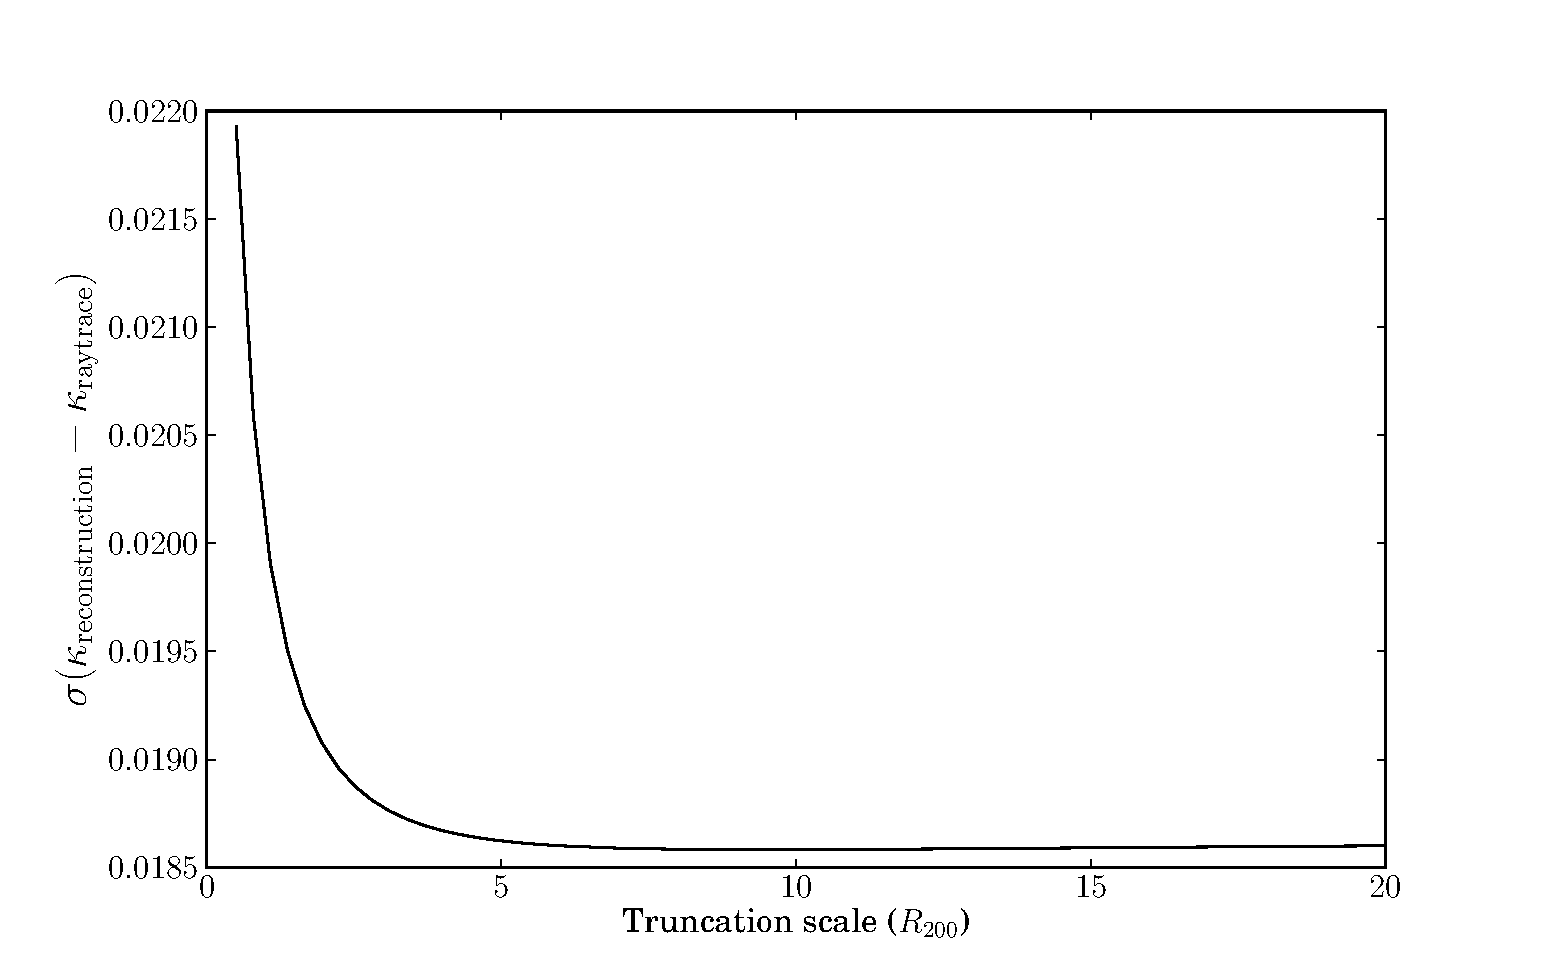
\includegraphics[width=\columnwidth]{figs/truncation_scatter.eps}
\caption[magcut]{The standard deviation in $\kapparec$ minus $\kapparay$ as a function of halo truncation radius in virial radii, using the truncated NFW profile of \citet{BMO}. In our models we truncate our halos at 5$R_{200}$}
\label{fig:ScattervsTruncation}
\end{figure}

For $\sumkappah$ to provide useful constraints on $\kapparay$, it is important that $\kapparay$ and $\sumkappah$ are as similar as possible. Figure \ref{fig:bias} shows that indeed $\sumkappah$ is a good estimator, regardless of the individual value of $\sumkappah$. At fixed $\sumkappah$ we find that the scatter in $\kapparay$ grows with $\sumkappah$; our reconstruction is better at reproducing underdense lines of sight than overdense lines of sight.

\begin{figure}
% 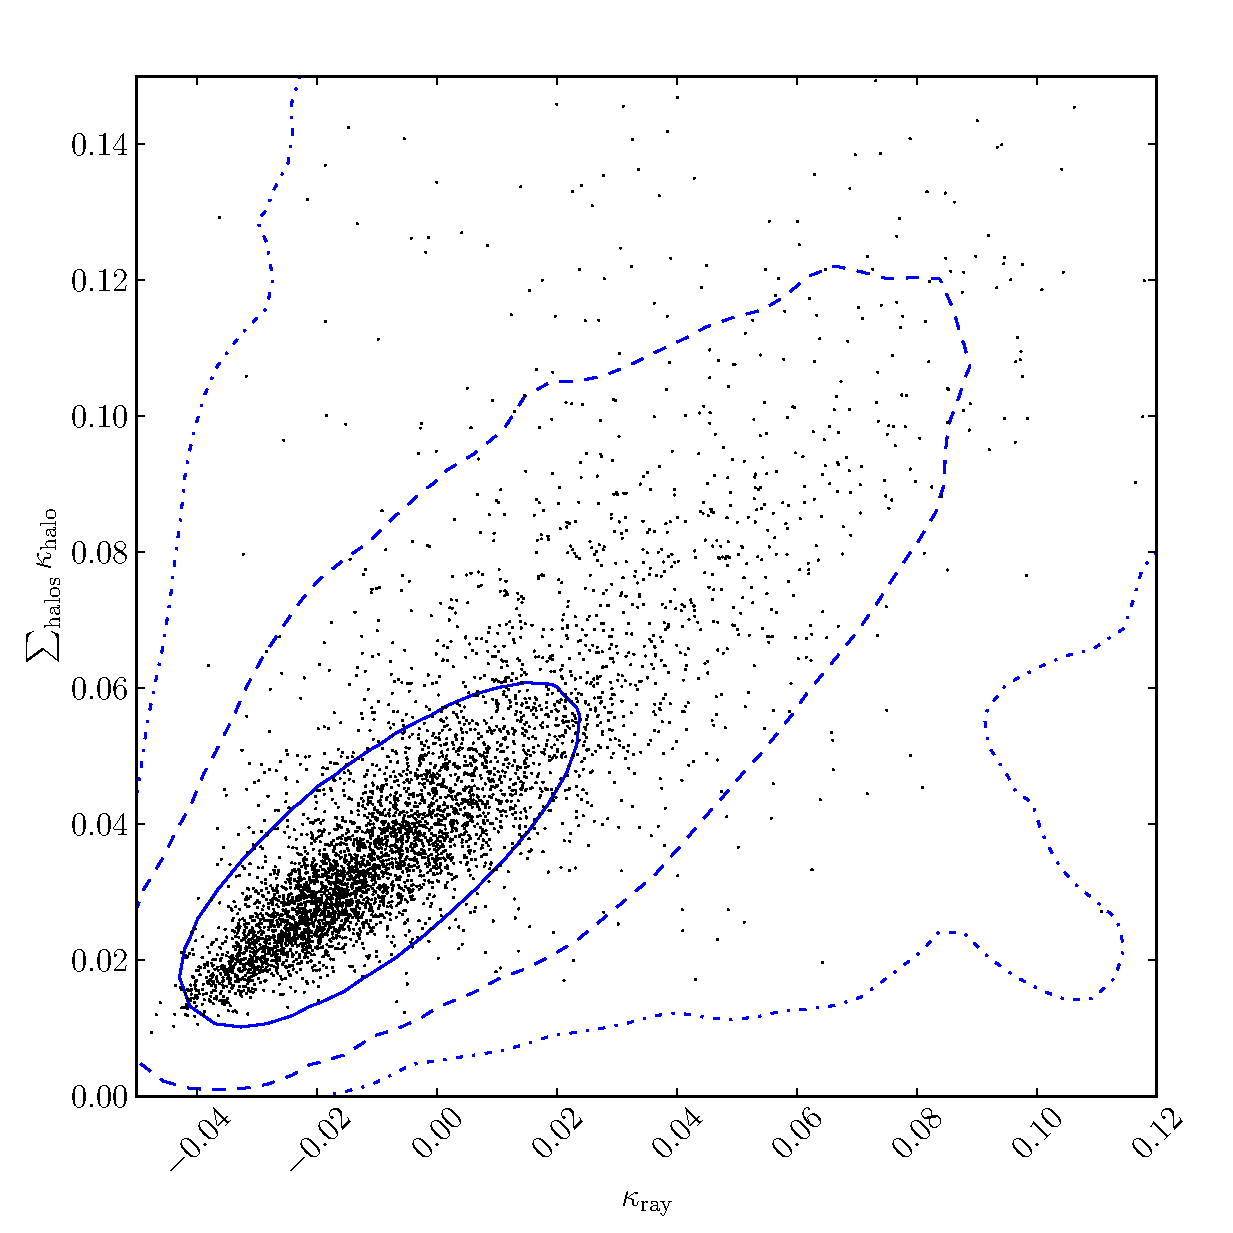
\includegraphics[width=\columnwidth]{figs/perfectc.eps}
\caption[Biased?]{$\sumkappah$ verses $\kapparay$ for 100000 reconstructed lines of sight. $\sumkappah$ traces $\kapparay$, but with a non-zero offset which is due to the negative connvergence from voids. At fixed $\sumkappah$ the scatter in $\kapparay$ grows with $\sumkappah$.}
\label{fig:isitbiased}
\end{figure}

The intrinsic error between the results of the halo based prescription and the raytraced convergence is an unavoidable error, even with perfect knowledge of halo mass and position. Before investigating the errors caused by imperfect knowledge of halo mass and redshift, we investigate the errors induced by a magnitude limited reconstruction and a field of view limited reconstruction. The halos in our catalogue are given magnitudes by the semi-analytic model of \citet{deLucia+Blaizot2007} and by applying magnitude cuts to our catalogue, we can investigate the scatter caused by unobserved halos. The majority of the convergence comes from halos with an $i$ magnitude between 18 and 24. Figure \ref{fig:magcut} shows that the width of $\kapparec-\kapparay$ decreases quickly between $i=18$ and $i=24$. Objects brighter than $i=18$ are either too rare or too close to the observer to make a significant contribution to the convergence. Objects fainter than $i=24$ are too small to be important, unless they are extremely close to the line of sight where it is likely that neglecting stellar mass and using a spherical NFW prescription are too naive to adequately reconstruct $\kappax$. It is likely that ultra-faint halos (or substructures), the uncertain contribution of voids and halos deviating from our spherical truncated NFW profile are the three major sources of the scatter in $\kapparec-\kapparay$; a deeper survey will not be sufficient to decrease the size of this scatter. Since a large number of callibration lines of sight must be reconstructed to sample $\pr(\kappav)$, it may prove unrealistic to reconstruct the calibration lines of sight out to 5 arcminutes. Figure \ref{fig:radcut} shows the width of $\kapparec-\kapparay$ as a function of reconstruction radius; in almost all cases there is no significant contribution to $\kappa$ from halos that are centred more than 1 arcminute away, although large groups or clusters can sometimes still make a contribution as far out as four arcminutes. For the rest of this work we will continue to model all of the halos out to 5 arminutes with an $i$ magnitude greater than 26, although a reconstruction with fields going out to two arcminutes and down to $i=24$ would do almost as well.

\begin{figure}
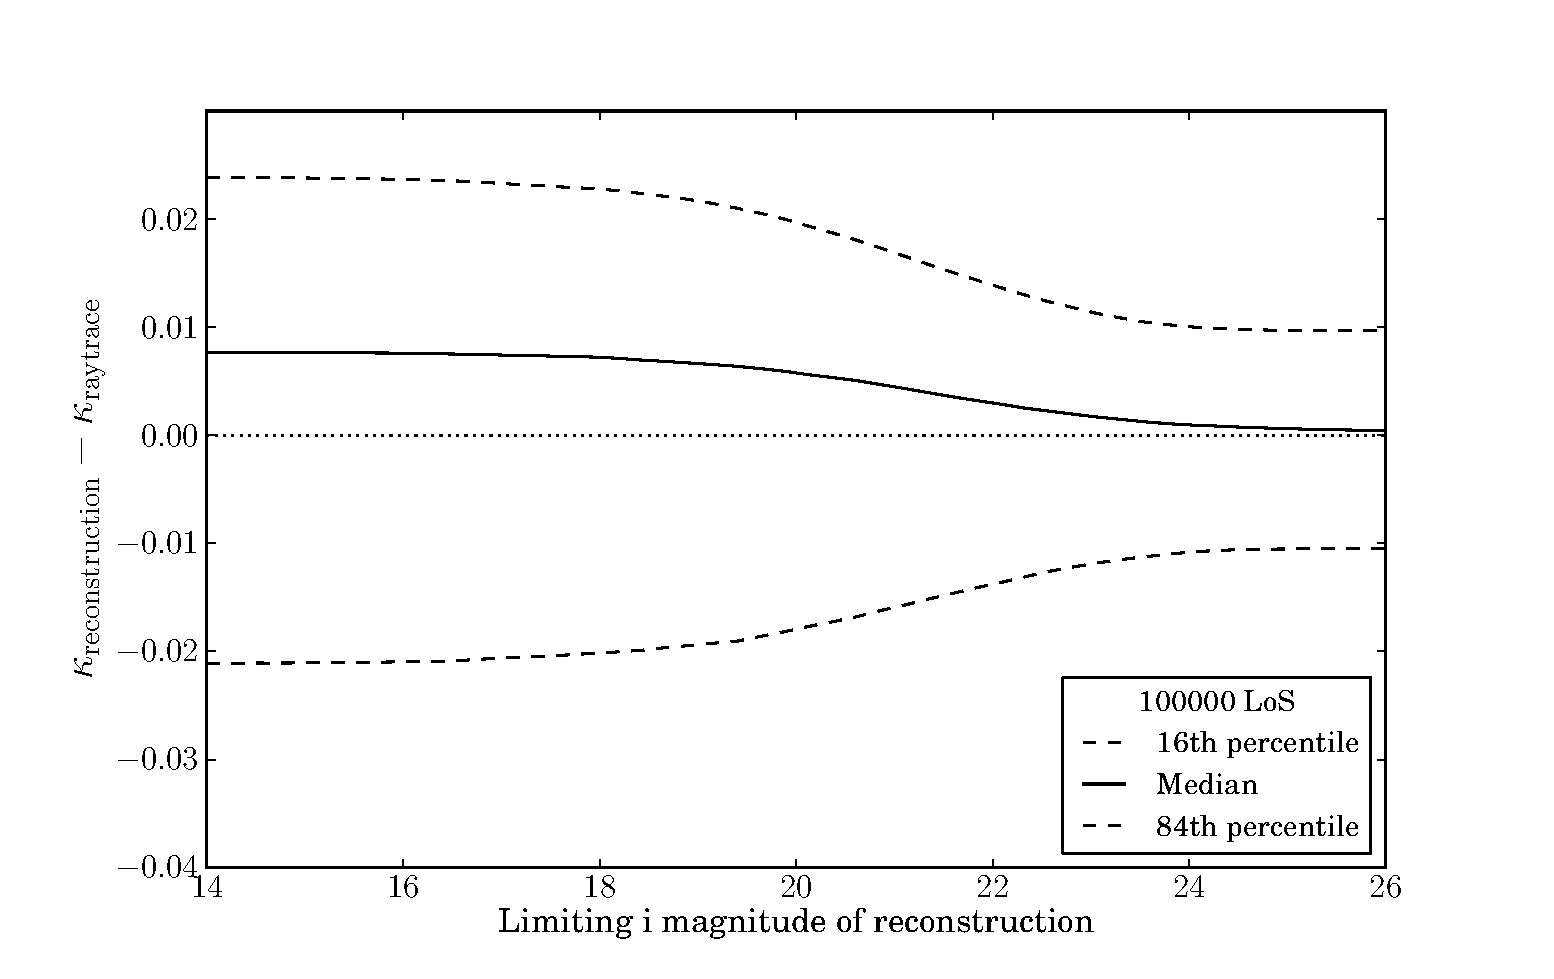
\includegraphics[width=\columnwidth]{figs/mag_scatter.eps}
\caption[magcut]{The 16, 50 and 84\% confidence intervals on $\kapparec$ minus $\kapparay$ as a function of the limiting $i$ band depth of the halo reconstruction. $\kapparec$ is given by $\sumkappah-\kappav$, where $\kappav$ is a constant such that $\left\langle\kapparec\right\rangle=0$. The majority of the constraining power comes from reconstructing halos with magnitudes between $18<i<24$}
\label{fig:magcut}
\end{figure}
\begin{figure}
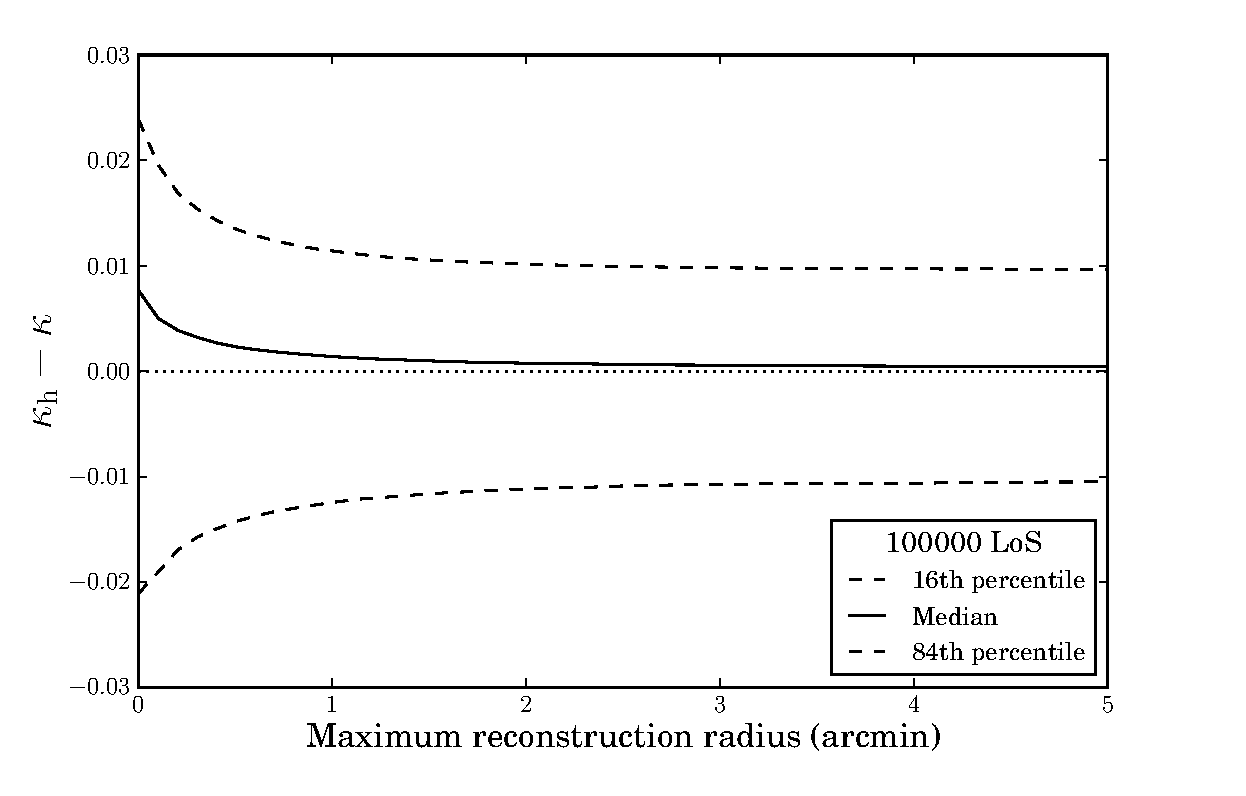
\includegraphics[width=\columnwidth]{figs/radius_scatter.eps}
\caption[radius cut]{The 16, 50 and 84\% confidence intervals on $\kapparec$ minus $\kapparay$ as a function of the limiting radius (in arcminutes) beyond which halos are not reconstructed. The majority of the convergence comes from halos centred within an arcminute of the line of sight}
\label{fig:radcut}
\end{figure}

The final test that we apply to the perfect knowledge reconstruction is to apply the marginalization outlined in Section \ref{subsec:voids}. Taking the reconstructed $\sumkappah$ for $1\times 10^{5}$ lines of sight we form the joint distribution, P$(\kapparay,\sumkappah)$ and marginalize over all sightlines with a similar $\sumkappah$ to give P($\kappax$). We define the bias as the difference between the expectation value of $\kappax$ and the known true value of $\kapparay$ for each Line of sight and we define the reconstruction width as half the width of the interval containing the central $68\%$ of the probability P($\kappax$). From $1\times 10^{4}$ reconstructed lines of sight we find the the bias to have mean of $-9.5\times 10^{-6}$ and a mean reconstruction width of 0.0132. In the case where one assumes P$(\kappax)$ is given by the global P$^{\rm global}(\kappax)$, the same $1\times 10^{5}$ lines of sight show a mean bias of $4.3\times 10^{-5}$ and mean reconstruction width of 0.237. Within the statistical error both methods are unbiased, but for any individual line of sight the bias is typically 1.8 times smaller with the reconstructed P$^{\rm reconstruction}(\kappax)$, rather than global P$^{\rm global}(\kappax)$. 

%%%%%%%%%%%%%%%%%%%%%%%%%%%%%%%%%%%%%%%%%%%%%%%%%%%%%%%%%%%%%%%%%%%%%%%%%%%%%%%%

\section{Tests on mock catalogs}
\label{sec:obsMstar+z}

Real attempts to reconstruct the convergence along a line of sight will not have direct access to the masses of dark matter halos, 
and will likely not have access to their spectroscopic redshift either. Instead these properties must be inferred from astrophysical
observables. In principle the only observables are astrometric positions, photometric colours and possibly spectra. In this section we
quantify the errors induced by inferring the halo mass and redshift from the observables. Much work has already focused on using
photometric colours to infer stellar mass \citep[\eg][]{xxx} and redshifts \citep[\eg][]{BPZ}, in line with these we shall use
stellar mass and photometric redshifts (with appropriate errors), as the observables that must be converted into an estimate
of $\kappax$. We will investigate two main sources of error: inferring halo mass given observed stellar mass and placing halos at the wrong redshift due to photometric redshift error.

We generate a stellar mass for each halo according to the stellar mass--halo mass relation of \citet{BehrooziEtal2010}. From this stellar mass we simulate 
an observed stellar mass by drawing a sample from $\pr(\log(M_{* \mathrm {obs}})|\log(M_{* \mathrm {true}}))$ which is given by \comments{ the product of the galaxy stellar mass function (GSMF) of \citet{Fontana2006} and} a Gaussian of width $\sigma_{M_*}$ centred on $\log(M*_{\mathrm {true}})$. Where a spectroscopic redshift exists stellar masses can be estimated with typical uncertainties of 0.15 dex \citep{xxx}, however with photometric redshifts stellar mass uncertainties are typically three times as large \citep{xxx}; we use $\sigma_{M_*}=0.15$ for halos with a spectroscopic redshift and $\sigma_{M_*}=0.45$ otherwise. \comments{The \citet{Fontana2006} GSMF is given by a Schechter function with redshift evolving parameters
\be
\label{eq:GSMF}
{\dee N \over \dee M_*} \propto \left(10^{(M_*-M_0(z))}\right)^{(1+\alpha(z))} \exp \left(-10^{(M_*-M_0(z))}\right)
\ee 
where $M_0(z)=11.16+0.17z-0.07z^2$ and $\alpha(z)=-1.18-0.082z$.} For photometric redshift errors we draw a redshift from $\pr(z_{\rm true}|z_{\rm obs})$ which we take as a Gaussian of width $0.1(1+z_{\rm spec})$ centred on $z_{\rm spec}$, where $z_{\rm spec}$ is the halo's true redshift in the \MS catalogue

For each  source of error, we reconstruct 40000 calibration lines of sight and 10000 mock lens lines of sight, following the proceedure outlined in Section \ref{sec:model}. Reconstructing the lines of sight with perfect knowledge of the redshift but an uncertain stellar mass, we find that the width of $\Pr\left(\sumkappah \right)$ grows with the expectation value of $\sumkappah$; this is not surprising since the low $\sumkappah$ lines of sight are relatively empty and so there are few opportunities for uncertainties in the halo masses to propogate into $\sumkappah$ uncertainties. After applying the void correction the expected bias from our 10000 mock lenses is $6.7\times 10^{-5}$ and the mean reconstruction width is 0.0145; this is the typical reconstruction error that could be expected from a complete spectroscopic survey of the field, it is ten percent worse than the reconstruction given perfect knowledge of the halo masses and redshifts but still 1.6 times better than using the global P$^{\rm global}(\kappax)$ although a complete spetroscopic survey is still unrealistic. The distribution of the widths of $\Pr\left(\kappax \right)$ is shown in Figure \ref{fig:width1}


\begin{figure}
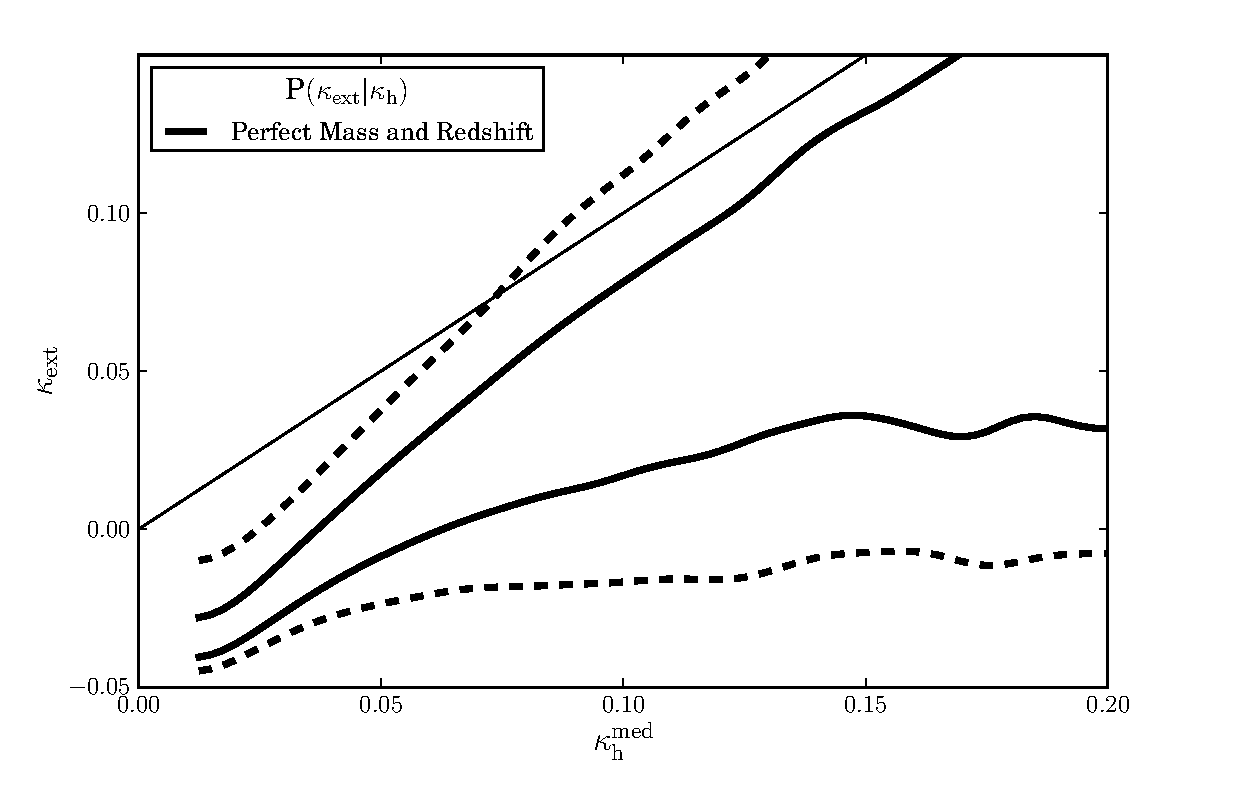
\includegraphics[width=\columnwidth]{figs/cornerplot.eps}
\caption{68 \% and 95 \% contours of the joint distribution $\pr(\kapparay, \tilde\kappa_{\rm halos})$ given a mock reconstruction of our 40000 calibration lines of sight. $\tilde\kappa_{\rm halos}$ is the median of $\pr(\sumkappah)$ given a spectroscopic redshift for each halo. $\kapparay$ and $\tilde\kappa_{\rm halos}$ are strongly correlated, despite the blurring effect of uncertain halo masses.}
\label{fig:corner}
\end{figure}

\begin{figure}
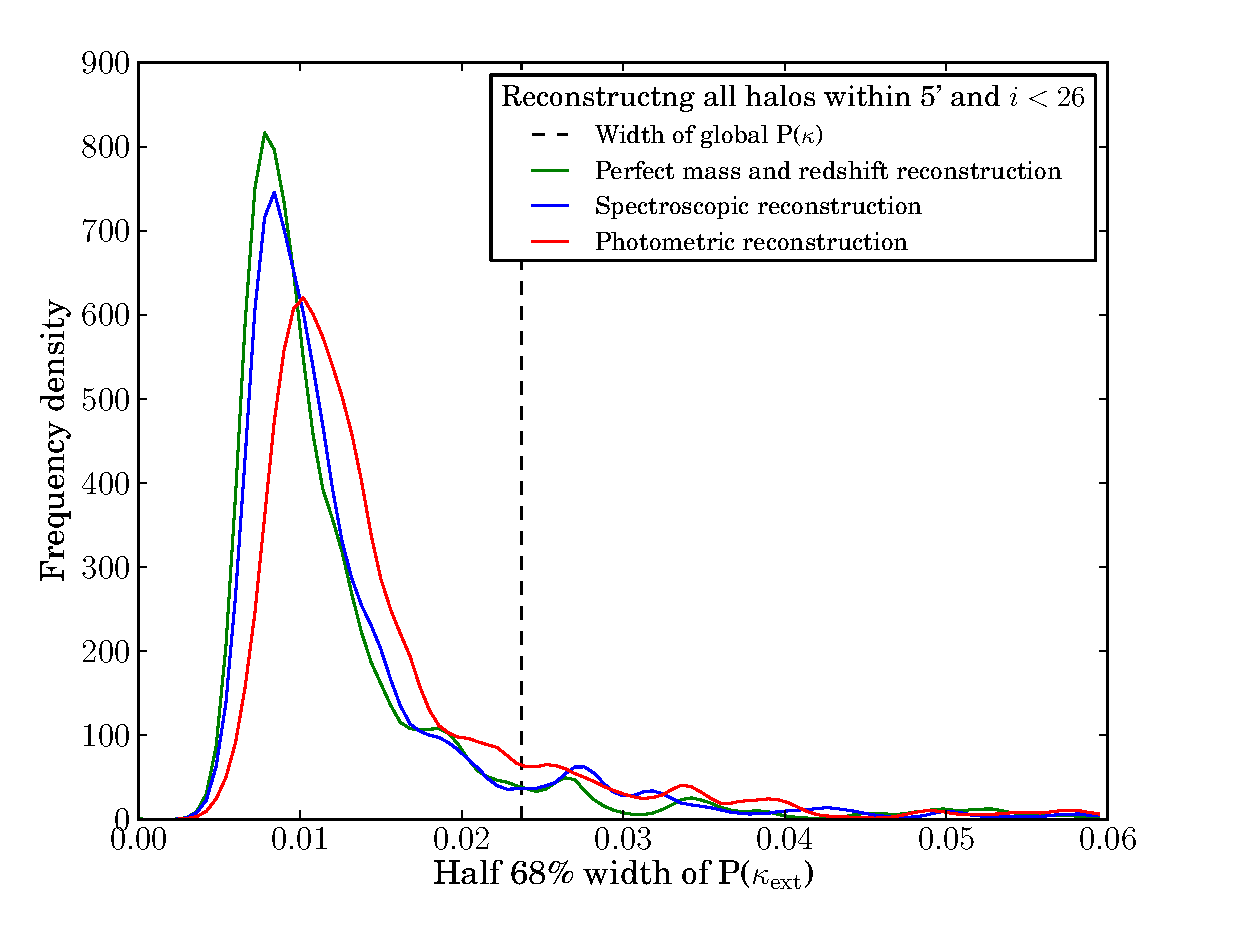
\includegraphics[width=\columnwidth]{figs/widths.eps}
\caption{Widths of $\pr(\kappax)$ after applying our reconstruction of all halos down $to i=26$ and within 5 arcminutes of the line of sight. Results for 10000 lines of sight are shown. Green is for a reconstruction given perfect knowledge of halo mass and redshift, blue is for a reconstruction given a spectroscopic redshift for every halo, and red is for a reconstruction with photometric redshifts only. The dashed black line shows the width of the global $\pr(\kappax)$ distribution; the reconstruction process provides roughly a factor of 2 improvement for the majority of lines of sight. Spectroscopic redshifts improve the reconstruction, but at signifcant observational cost.}
\label{fig:width1}
\end{figure}

Inferring the stellar mass of a galaxy from its magnitude and colours requires an estimate of how far away the galaxy is; without a spectroscopic redshift the the infered stellar mass is less precise. In principle the photometric redshift is correlated with the infered stellar mass, however we do not model this effect since the convergence from the outskirts of an individual halo is only weakly dependant on redshift at fixed mass: the redshift error is small effect on the recovered $\pr(\kappa)$ when compared to the effect of uncertain stellar masses.  With only photometric redshifts the uncertainty on $\sum\kapparec^{\rm halos}$ is much larger than the spectrocopic case, but this does not propogate into a much larger bias after applying the void correction; with a purely photometric reconstruction of the 10000 mock lightcones the results have a mean bias of $1.1\times 10^{-4}$ and a mean width of 0.0158. On average a purely photometric reconstruction of the field gives an unbiased $\pr(\kappax)$ that is 1.5 times tighter than assuming the global $\pr^{\rm global}(\kappax)$. 


\subsection{Reconstructions of Smaller and Shallower Fields}

\begin{figure}
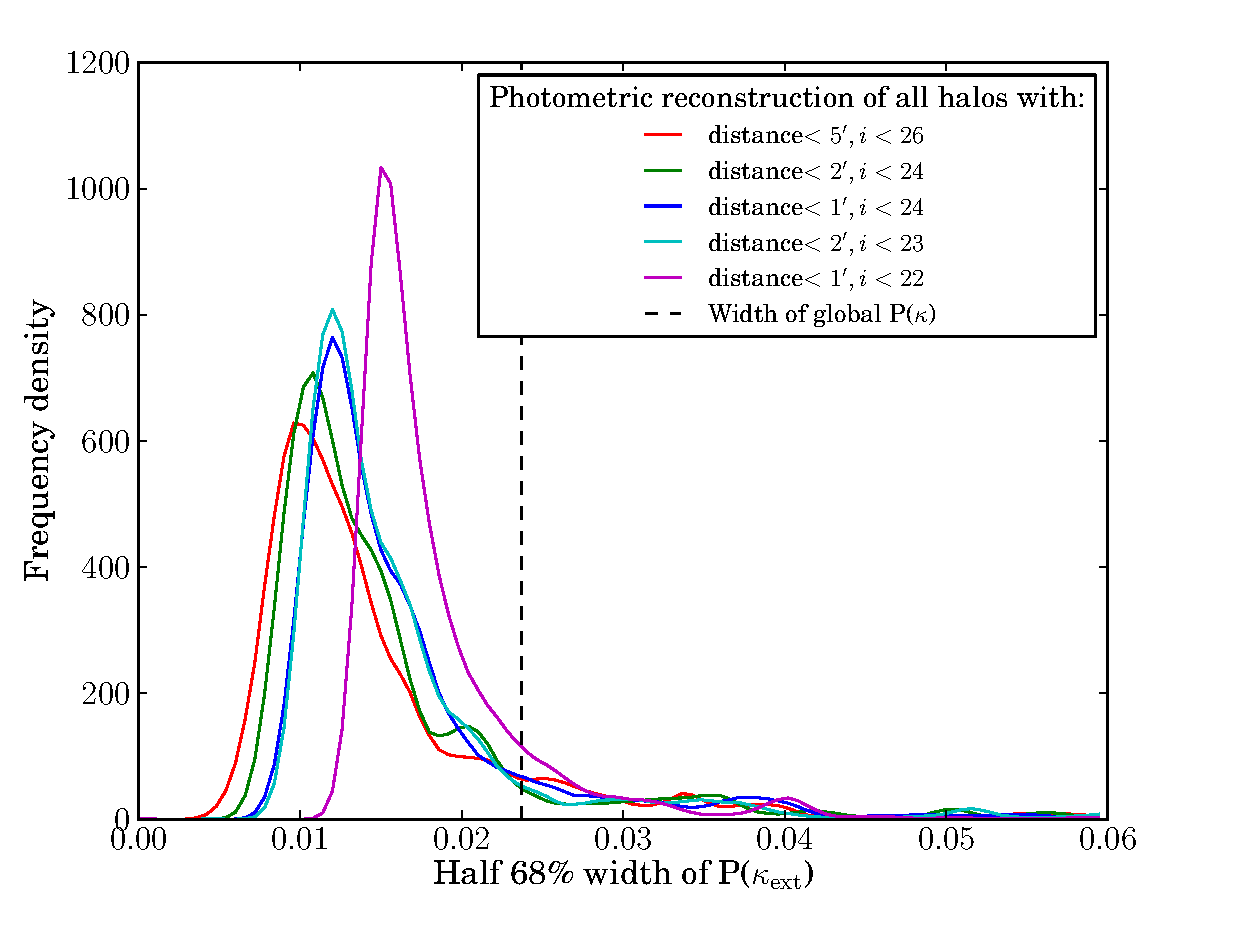
\includegraphics[width=\columnwidth]{figs/widths2.eps}
\caption{Widths of $\pr(\kappax)$ after a photometric reconstruction of all halos within different fields. The different field sizes and depths are given in the legend. As the field becomes smaller or shallower, fewer halos are being reconstructed and so the width of $\pr(\kappax)$ grows.}
\label{fig:width2}
\end{figure}


Reconstructions of real lines of sight may not have access to the deep, large calibration fields that we have used upto this point. We can perform the same reconstruction but for a more modest mock survey. Given the results of Section \ref{sec:knownMh+z} we predicted that a reconstruction of the field out to 2 arcminutes and a magnitude limit of $i$=24 would provide similar constraints to a reconstruction going out to 5 arcminutes and going down to $i$=26. We find the mean reconstruction width to be 0.0163 for a photometric reconstruction of all the halos within 2 arcminutes that have $i<24$, this is only marginally worse than 0.0158 which was the typical width after the deeper and wider reconstruction of the previous section. The reconstruction widths for our 10000 mock lens lines of sight are shown in Figure \ref{fig:widths2}. If only photometry for halos with $i<24$ and within 1 arcminute of the line of sight is availble then the typical width of the reconstructed $\pr(\kappax)$ is 0.173. Whilst a complete spectroscopic survey of a large field would be unlikely, a hybrid strategy of obtaining spectra for a subset of objects may be feasible. Photometric redshifts are sufficient to asertain the halos which are likely to contribute most of the convergence on any given line of sight, and on average there are only $\sim 6 \pm 6$ halos per line of sight that individually contribute more than 0.002 to $\sumkappah$. We investigate a hybrid strategy of obtaining spectroscopic redshifts for all of the $i<24$ halos which contribute an individual $\kappa$ of at least 0.002 combined with a photometric redshift for all other $i<24$ halos within 2 arcminutes. For the hybrid strategy the typical width of the reconstructed $\pr(\kappax)$ is 0.0151. The observational cost of obtaining spectroscopic redshifts for several 24th magnitude galaxies may make the hybrid strategy unlikley, but obtaining photometry of a 4$\times$4 arcminute patch of sky down to $i=24$ is fast with modern telescopes. The mean reconstruction width for a photometric reconstruction of all the halos within 2 arcminutes that have $i<24$ represents an improvement of 1.5 over using the global $\pr(\kappax)$ and should be achievable at minimal observational cost.

%\subsection{Reconstructing Biased Lines of Sight}


%%%%%%%%%%%%%%%%%%%%%%%%%%%%%%%%%%%%%%%%%%%%%%%%%%%%%%%%%%%%%%%%%%%%%%%%%%%%%%
\comments{
\section{Time Delay Distances}
\label{sec:Dt} 

Folding the kappa uncertainties into time delay distance uncertainties. Toy
model: same zl and zs, allows simple product of pdfs to obtain estimate of P(D).

Make mock sample of lenses, all wit B1608 zd and zs, but with different kappas.
Draw kappas from Stefan's *lens* distribution. Can we correct for the selection
effect?

% % % % % % % % % % % % % % % % % % % % % % % % % % % % % % % % % % % % % % %

\subsection{Comparison with Other Treatments of $\kappax$}
\label{sec:Dt:selection} 

\phil{How does distance accuracy compare with simple averaging? eg assuming
$\kappax = 0$ for all lenses. How does it compare with the no data situation?
eg where the intrinsic distribution of kappa is used as $Pr(\kappax)$.}

What is the expected bias and scatter (centroid position and width) of P(D) as a
function of N lenses? How does reconstruction compare with P(D) derived using
P(kappa|N45) for each lightcone? How does reconstruction compare with P(D)
derived assuming kappa=0 for each lightcone?

Also: compare with simple averaging. This will fail if lenses are selected to
live on over-dense lines of sight. Stefan's plot in Suyu et al shows effect of
selection - what is the resulting bias? Few percent? This is the target to beat,
need to find it out.


% % % % % % % % % % % % % % % % % % % % % % % % % % % % % % % % % % % % % % %

\subsection{The Impact of Selection Effects}
\label{sec:Dt:selection} 

\phil{How does distance accuracy vary with:}
\begin{itemize}
\item Depth of catalog? mlim = 22, 24, 26?
\item Overdensity cuts? Remove underdense fields, overdense fields (from
reconstructed kappa)
\item Shear-sensitive selection? What if we only selected quads?
\end{itemize}


% % % % % % % % % % % % % % % % % % % % % % % % % % % % % % % % % % % % % % %

\subsection{Improving the Accuracy with More Information}
\label{sec:Dt:selection} 

\phil{How does distance accuracy improve with:}
\begin{itemize}
\item Spectroscopic coverage? For galaxies above some mlim? For targets with
high kappa contribution (based on photometry)?
\item IR coverage for all objects? Improves photo-z and Mstar.
\item Including shear information from lens model? Assume accurate but
uncertain extertanl shear.
\end{itemize}


% %%%%%%%%%%%%%%%%%%%%%%%%%%%
% \begin{figure}
% \centering\includegraphics[width=0.99\linewidth]{figs/something.png}
% \caption{An example figure.}
% \label{fig:sizemass}
% \end{figure}
% %%%%%%%%%%%%%%%%%%%%%%%%%%%

}
%%%%%%%%%%%%%%%%%%%%%%%%%%%%%%%%%%%%%%%%%%%%%%%%%%%%%%%%%%%%%%%%%%%%%%%%%%%%%%

\section{Discussion}
\label{sec:discuss}

We have shown that reconstructing the matter due to halos along any line of sight can give meaningful and unbiased constraints on the external convergence along that line of sight. The total convergence along a line of sight is strongly correlated with the reconstructed $\sumkappah$. However since our model ignores voids and assumes all halos follow a spherical truncated-NFW profile our model does not include all of the relevant physics, hence the width of our resulting $\pr(\kappax)$ is still typically $\sim$0.01, even with a perfect knowledge of every halo's virial mass and redshift. To make further progress a more advanced treatment of both voids and halos will be necessary. Interestingly, we have found that the most empty lines of sight can be reconstructed with the most precision. $\kappax$ for empty lines of sight have little contributions from halos and a large contribution from voids; since they have the tightest PDFs after the reconstruction it seems that our model's biggest uncertainties are driven by naively reconstructing halos rather than neglecting voids. With a photometric reconstruction of the field there is only a small broadening compared to the perfect knowledge reconstruction; it seems that deviations from sphericity and dark matter clumping within the main halo are the dominant uncertainies rather than uncertainties in the halo mass. Inferring halo ellipticity and dark matter clumping will likely always remain a difficulty for line of sight reconstruction; as Figures \ref{fig:magcut} and \ref{fig:width2} show observing deeper than 24th magnitude does not signifcantly help the reconstruction. Because our reconstruction is mostly limited by the model, spectroscopic coverage can only provide a modest improvement to the reconstruction and at significant observational cost.

For a small fraction of lines of sight, $\pr(\kappax)$ remains very broad even after applying our reconstruction; these lines of sight are typically the most overdense lines of sight in the universe. For time-delay cosmography the most observationally expensive task is the lightcurve monitoring, whilst making photometric observations of a 4$\times$4 arcminute patch of sky survey down to 24th magnitude is a relatively cheap. We have shown that with a single epoch observation of the region around a strong lens it is possible to infer $\pr(\kappax)$. If a line of sight has a broad $\pr(\kappax)$ it can be rejected {\it before} the investment of longterm lightcurve monitoring.

The method we have outlined can also be used to estimate the external shear
along a line of sight. Shear is an observable that can be extracted from
strong lens modelling, however there is a degeneracy between internal and
external shear. Progress has been made in disentangelling external and
internal shear \citep[\eg][]{xxx} but there are still significant
uncertainties: \citet{WongEtal2011} attempted to match the shear from strong
lens models with a reconstruction of the local lens group environment, but
found a tension between the strong lens model and the reconstruction of the
environment. Since \citet{WongEtal2011} only reconstructed the local lens
group, rather than the full line of sight contribution, it is unclear whether
the external shear from lens models can be reconciled with a line of sight
reconstruction. {\it If} external shear can be measured, it provides an
additional constraint on which of the Millenium Simulation lines of sight are
similar to the reconstructed line of sight. \citet{SuyuEtal2012} found that
for RXJ1131 combining shear constriants with galaxy number count overdensity,
gave a significantly different $\pr(\kappax|\gamma,N_{45})$ copmpared to the
PDFfrom number count overdensity alone, $\pr(\kappax|N_{45})$. 



%%%%%%%%%%%%%%%%%%%%%%%%%%%%%%%%%%%%%%%%%%%%%%%%%%%%%%%%%%%%%%%%%%%%%%%%%%%%%%

\section{Conclusions}
\label{sec:conclude}

In this work we have investigated a simple halo model prescription for
reconstructing all the mass along a line of sight to an intermediate redshift
source. We have used the ray-traced lensing convergence along lines of sight
through the Millenium Simulation to test this approach, and to calibrate
estimates of the total convergence along a line of sight to an observed
distant galaxy made by summing the convergences due to each object in a
photometric catalogue. Having found that the reconstruction process is effective given perfect
knowledge of halo mass and redshift, we investigated the effects of reasonable
uncertainties in the stellar mass and redshift of each halo, and propogated
these uncertainties into a $\pr\left(\sumkappah\right)$ for each line of
sight. We draw the following conclusions:

\begin{itemize} 

\item Our model uses a truncated spherical NFW profile for
each dark matter halo and neglects voids, but despite the model's simplicity
the reconstructed $\sumkappah$ is a good tracer of $\kappax$.  We found that
with perfect knowledge of the halo mass and redshift (from the Millenium
Simulation catalogs), the reconstruction gives an unbiased estimate of
$\pr(\kappax)$ for a single line of sight that is almost almost a factor of 2
less broad than the global $\pr(\kappax)$. 

\item  For the most overdense lines of sight, the reconstruction produces a
very broad PDF, but since the reconstruction can be performed before follow-up
time is invested it will be possible to discard the most uncertain lines of
sight and prevent the waste of follow-up time. 

\item With complete spectroscopic redshift coverage and just an empirical
stellar mass to halo mass relation, we find that the median of
$\pr\left(\sumkappah\right)$ is a useful indicator for generating an estimate
of $\pr(\kappax)$ from the ensemble of simulated lines of sight. The resulting
PDF tends to be around 10\% broader than it would have been given perfect
knowledge of both halo mass and redshift; given only photometric redshifts
(which in turn give rise to much less certain stellar masss estimates) causes
another $\sim$10\% increase to the width of $\pr(\kappax)$.

\item It is very rare for halos further than 2 arcminutes to make a
significant contribution to $\kappax$. We also found that including halos
whose host galaxy is less luminous than $i=24$ does not significantly improve
our reconstruction proceedure. A photometric survey to this depth of a
4$\times$4 arcminute patch around the lens would approach the limiting
uncertainties of our simple reconstruction recipe, and yield a 
$\pr(\kappax)$ that has, on average, a width of 0.0163 --
50\% less broad than the global $\pr(\kappax)$.

\item We find that the lines of sight with the sharpest $\pr(\kappax)$ are
typically under-dense. With a photometric reconstruction of all lens fields,
and following up only the lenses with the most constraining $\pr(\kappax)$,
the width of the dominant statistical uncertainty in time-delay cosmography
can be halved, whilst at the same time decreasing any potentail for a
systematic error due to lenses being biased in $\kappax$.

\end{itemize}

\todo{Tom}{Add more conclusions about bias in a large sample of lenses...}

\todo{Tom}{Wrap up}


%Our conclusions can be summarised as follows:
%\begin{itemize}
%\item With perfect 
%\item And we found this too.
%\end{itemize}

% \item Faint galaxies and other dark structures will not appear in a photometric
% object catalog, but they will contribute convergence at some level. How much of
% the total external convergence in a time delay lens system comes from visible
% galaxies? How does this change as a function of magnitude cut? 

% \item Can the true (ray-traced) convergence be recovered by halo model
% reconstruction, and with what scatter and residual bias? Which aspects of the 
% model dominate these uncertainties?

% \item When faced with a newly-detected lens, surrounded by galaxies on the sky,
% we have some choices to make when planning follow-up observations.
% Which are the most important galaxies, with regard to the external convergence
% produced? Can nearby groups and clusters be straightforwardly accounted for? If
% lenses with such massive structures nearby are discarded, what impact does that
% have on the distance accuracy?



%%%%%%%%%%%%%%%%%%%%%%%%%%%%%%%%%%%%%%%%%%%%%%%%%%%%%%%%%%%%%%%%%%%%%%%%
%%  ACKNOWLEDGMENTS
%%%%%%%%%%%%%%%%%%%%%%%%%%%%%%%%%%%%%%%%%%%%%%%%%%%%%%%%%%%%%%%%%%%%%%%%

\section*{Acknowledgments}
 
TC thanks Vasily Belokurov for guidance and discussions.
We thank Risa Wechsler and Peter Behroozi for useful discussions and 
suggestions.
TEC acknowledges support from STFC in the form of a research studentship.
%
PJM was given support by the Kavli Foundation and the Royal 
Society, in the form of research fellowships.
%
MWA \ldots
%
SH \ldots
%
SHS \ldots
%
TT acknowledges support from the NSF through CAREER award NSF-0642621,
and from the Packard Foundation through a Packard Research Fellowship.
% 
LVEK acknowledges the support by an NWO-VIDI programme subsidy
(programme number 639.042.505).
%
This research is supported in part by the National Science Foundation under
Grant No. PHY99-07949.



%%%%%%%%%%%%%%%%%%%%%%%%%%%%%%%%%%%%%%%%%%%%%%%%%%%%%%%%%%%%%%%%%%%%%%%%%%%%%%
%  APPENDICES
%%%%%%%%%%%%%%%%%%%%%%%%%%%%%%%%%%%%%%%%%%%%%%%%%%%%%%%%%%%%%%%%%%%%%%%%%%%%%%

\appendix

%%%%%%%%%%%%%%%%%%%%%%%%%%%%%%%%%%%%%%%%%%%%%%%%%%%%%%%%%%%%%%%%%%%%%%%%%%%%%%

\section{Truncated NFW halos}
\label{appendix:halos}

 Defining $x$ as the dimensionless projected radial distance $R/r_{s}$ and $\tau$ as the dimensionless truncation radius $r_{t}/r_{s}$, \citet{BMO} derives the projected mass density, which is given by:
\begin{align}\label{eq:kappaBMO}
\Sigma_{\rm}(x) = {2\tau^2 \over (\tau^2+1)^2}\left(
        {\tau^2+1\over x^2-1}\left(1-\mathcal{F}(x)\right)
        +
        2\mathcal{F}(x)\right.\nonumber\\
        -
        \left. {\pi \over \sqrt{\tau^2+x^2}}
        +
        {(\tau^2-1)\mathcal{L}(x,\tau)
        \over
        \tau\sqrt{\tau^2+x^2}}\right)
\end{align}
where $\mathcal{F}(x)$ and $\mathcal{L}(x,\tau)$ are defined as
\be\label{eq:F} 
\mathcal{F}(x) \equiv \begin{cases}  \frac{{\rm cos}^{-1} (1/x)}{\sqrt{x^2-1}} \hspace{0.2cm} & (x>1) \\
\\
\frac{4-x^2}{3}  & (x=1)\\
\\
\frac{ {\rm cosh}^{-1} (1/x)}{\sqrt{1-x^2}} & (x<1)
\end{cases}
\ee
\be\label{eq:L}
\mathcal{L}(x,\tau) = \ln\left(\frac{x}{\sqrt{\tau^2+x^2}+\tau}\right)
\ee
%the convergence is given by $\Sigma_{\rm BMO}(x) / \Sigma_{\rm cr}(z)$.



%%%%%%%%%%%%%%%%%%%%%%%%%%%%%%%%%%%%%%%%%%%%%%%%%%%%%%%%%%%%%%%%%%%%%%%%%%%%%%

\section{Inferring $\Mhalo$ given a noisy measurement of $\Mstarobs$}
\label{appendix:MSMH}

Given a noisy estimate of the stellar mass $\Mstarobs$ of a galaxy at redshift
$z$, how can we infer the galaxy's halo mass? We then seek the posterior
PDF $\Pr(\Mhalo|\Mstarobs)$, which can be expanded as follows:

\begin{eqnarray}
&& \Pr(\Mhalo|\Mstarobs,z) = \notag\\
&& \int d\Mstar \Pr(\Mhalo|\Mstar,z) \Pr(\Mstar|\Mstarobs,z), \notag\\
&\propto& \int d\Mstar \Pr(\Mstarobs|\Mstar) \Pr(\Mstar|\Mhalo,z) \Pr(\Mhalo|z),
\label{eq:mhalo-mstar}
\end{eqnarray}
where we have used Bayes' Theorem twice to replace
$\Pr(\Mhalo|\Mstar,z) \Pr(\Mstar|z)$ with 
$\Pr(\Mstar|\Mhalo,z) \Pr(\Mhalo|z)$, and 
to invert $\Pr(\Mstar|\Mstarobs)$ into the sampling
distribution $\Pr(\Mstar|\Mstarobs)$, which we recognise as the likelihood
function for the observed stellar mass. Note that the ``true'' $\Mstar$ of the
galaxy is marginalised out: we are only interested in reconstructing the halo
mass. The last two terms in
\eqref{eq:mhalo-mstar} are the $\Mstar-\Mhalo$ relation from
\citet{BehrooziEtal2010}, and the halo mass function $\Pr(\Mhalo|z)$, at the
given redshift. We can
tabulate the product of these two from our Millenium Simulation catalog,
constructing a two-dimensional histogram of halo masses and their associated
true stellar masses (drawn from the Behroozi relation). 

For each galaxy, we compute the likelihood function for its $\Mstarobs$ as a
function of the unknown $\Mstar$, and multiply it by our tabulated joint PDF.
This heavily downweights halos with $\Mstar$ values outside the observed
range. We then do the marginalisation integral by Monte Carlo, drawing
(two-dimensional) sample parameter vectors
from the downweighted histogram, discarding the $\Mstar$ values, and
constructing a one-dimensional histogram that is an estimate of
$\Pr(\Mhalo|\Mstarobs)$.

\todo{Matt}{Edit the above text to add a note on how we do the sampling in
practice, via the CDF.}

If the redshift of the galaxy is uncertain, we need to take this uncertainty
into account; for example, for each sample drawn from the photometric redshift
posterior PDF $\Pr(z|{\rm colors})$, we can draw a sample $\Mhalo$ using the
above procedure.


%%%%%%%%%%%%%%%%%%%%%%%%%%%%%%%%%%%%%%%%%%%%%%%%%%%%%%%%%%%%%%%%%%%%%%%%%%%%%%

\section{Accounting for uncatalogued low mass halos, and voids}
\label{appendix:smooth}

Our halo model allows us to infer a halo mass $\Mhalo$ for each galaxy in a
photometric catalog; under the weak lensing approximation described in
\Sref{sec:theory} we can compute the contribution of each of these halos to
the overall convergence and shear amplitude, assuming a homogeneous
Friedman-Robertson-Walker metric and the concordance $\Lambda$CDM cosmological
parameters for the angular diameter distances to calculate the critical
density for each lens plane. Clearly this approach will tend to over-estimate
the convergence, since we are placing massive halos into a volume that has
already been assumed to be full of homogeneously distributed matter with the 
mean cosmological density. In practice, the space between massive halos will
contain a) low mass halos that are not bright enough to be detected and b)
empty space where the density is below that of the mean. A rigorous treatment
of this complex situation is beyond the scope of this paper, but is being
investigated (Blandford et al, in preparation). In this appendix we describe
our empirical approach to accounting for the missing mass and voids. 

Let the summed convergence due to halos in our galaxy catalog be $\kappah$.
Given some assumptions about halo density profile and shape, this parameter
can be inferred from a set of uncertain halo mass estimates (which have in
turn been inferred from noisy measurements of galaxy redshift and stellar mass
as described in \Aref{appendix:MSMH}). We assume each halo to be a
spherically-symmetric NFW profile, and neglect the contribution of the stellar
mass to the convergence. The halo mass inference for the $k^{\rm th}$ galaxy 
is stored as a list of sample values of $\Mhalok$ drawn from the posterior PDF
$\Pr(\Mhalok|\Mstarobsk,z_k)$; computing the contribution to the convergence
due to this halo at the target line of sight for each sample gives, in turn, 
a set of
samples drawn from the PDF $\Pr(\kappahk|\Mstarobsk,z_k)$. We then generate
samples from $\Pr(\kappah|\{\Mstarobsk,z_k\})$ by drawing a sample $\kappahk$
for each halo, summing over halos to get $\kappah$, discarding those
samples and moving down the lists.

The PDF $\Pr(\kappah|\{\Mstarobsk,z_k\})$ will, in general, be broad (due to
the uncertainties involved in halo mass estimation). It will also be shifted
towards high values of convergence, due to the FRW approximation described
above. What we really want is an inference of $\Pr(\kappa|\{\Mstarobsk,z_k\})$
instead. We can obtain this by considering the expansion:
\begin{equation}
\Pr(\kappa|\{\Mstarobsk,z_k\}) = \int d\kappah 
   \Pr(\kappa|\kappah) \Pr(\kappah|\{\Mstarobsk,z_k\})
\label{eq:kappaconv}   
\end{equation}
The first term in the integrand relates the summed  convergence due to model
halos, $\kappah$, to the true summed convergence, $\kappa$.  In the Millenium
Simulation catalogs, we can compute a single value of $\kappah$ for each
selected line of sight from the true halo mass and redshift (and our same
assumptions of halo profile and shape), and tabulate the two-dimensional PDF
$\Pr(\kappa|\kappah)$ as a sequence of one-dimensional PDFs for $\kappa$ in a
bin at fixed $\kappah$. Note that this PDF captures the ``intrinsic scatter''
of $\kappah$ due to our assumptions about the clumpiness of mass in the
Universe; the integral is the convolution of this distribution with that
arising from our observational uncertainties.

For any given observed catalog then, we infer
$\Pr(\kappah|\{\Mstarobsk,z_k\})$ as described above, and then
multiply it by $\Pr(\kappa|\kappah)$; we
again do the marginalisation over $\kappah$ by Monte Carlo, drawing samples
from the two-dimensional grid and keeping only the $\kappa$ values, to form
our final result, $\Pr(\kappa|\{\Mstarobsk,z_k\})$. 
This PDF will describe, by construction, an accurate (i.e., unbiased)
measurement of $\kappa$ in the case where the Millenium Simulation halo
catalog and Behroozi et al $\Mstar-\Mhalo$ relation are themselves accurate
descriptions of galaxies and their distribution. In \Sref{sec:tests} we
investigate the amplitude of the systematic errors incurred if these
assumptions are not valid.

\todo{Matt}{Add text describing whatever sampling shortcut you derive! :-)}

% Finally, we note that \Eref{eq:kappaconv} and the method for evaluating the
% integral in it can be generalized to yield 
% $\Pr(\kappa,|\gamma||\{\Mstarobsk,z_k\})$, where $|\gamma|$ is the amplitude
% of the complex shear. The amplitude of the shear due to halos, $|\gammah|$ is
% needed in this calculation, and marginalised over -- $\gammah$ is computed by
% simple summation of its components, as in \Sref{sec:theory}. In
% \Sref{sec:includinggamma} we explore the impact that knowing $\gamma$ (from,
% for example, a strong lens model)  has on the inference of $kappa$, and how
% severe the systematic errors from getting this wrong might be.


%%%%%%%%%%%%%%%%%%%%%%%%%%%%%%%%%%%%%%%%%%%%%%%%%%%%%%%%%%%%%%%%%%%%%%%%%%%%%%
%  REFERENCES
%%%%%%%%%%%%%%%%%%%%%%%%%%%%%%%%%%%%%%%%%%%%%%%%%%%%%%%%%%%%%%%%%%%%%%%%%%%%%%

% MNRAS does not use bibtex, input .bbl file instead. 
% Generate this in the makefile using bubble script in scriptutils:

% bubble -f paper-lcr.tex references.bib 
% %%%%%%%%%%%%%%%%%%%%%%%%%%%%%%%%%%%%%%%%%%%%%%%%%%%%%%%%%%%%%%%%%%%%%%%%
%
% Pangloss: Testing the reconstruction method
%
%%%%%%%%%%%%%%%%%%%%%%%%%%%%%%%%%%%%%%%%%%%%%%%%%%%%%%%%%%%%%%%%%%%%%%%%

\documentclass[useAMS,usenatbib,a4paper]{mn2e}
%% letterpaper
%% a4paper

%\voffset=-0.6in

% Packages:
\input psfig.sty
\usepackage{xspace}
\usepackage{graphicx}
\usepackage{amssymb}
\usepackage{amsmath}

% Macros:
% JOURNALS
\newcommand{\apj}{ApJ}
\newcommand{\apjl}{ApJL}
\newcommand{\apjs}{ApJS}
\newcommand{\mnras}{MNRAS}
\newcommand{\apss}{Ap \& SS}
\newcommand{\aap}{A\&A}
\newcommand{\aj}{AJ}
\newcommand{\prd}{Phys. Rev. D}
\newcommand{\nat}{Nature}
\newcommand{\araa}{ARA\&A}
\newcommand{\jgr}{J. Geophys. Res.}
\newcommand{\pasp}{PASP}

% MISC
\newcommand{\etal}{et~al.~}
\def\spose#1{\hbox  to 0pt{#1\hss}}  
\newcommand{\lta}{\mathrel{\spose{\lower 3pt\hbox{$\sim$}}\raise  2.0pt\hbox{$<$}}}
\newcommand{\gta}{\mathrel{\spose{\lower  3pt\hbox{$\sim$}}\raise 2.0pt\hbox{$>$}}}
\newcommand{\eg}{{\it e.g.\ }}
\newcommand{\ie}{{\it i.e.\ }}
\newcommand{\be}{\begin{equation}}
\newcommand{\ee}{\end{equation}}
\newcommand{\dee}{\, \mathrm{d} \!}
\newcommand{\bea}{\begin{eqnarray}}
\newcommand{\eea}{\end{eqnarray}}


% CROSS-REFERENCING
\def\Sref#1{Section~\ref{#1}\xspace}
\def\Fref#1{Figure~\ref{#1}\xspace}
\def\Tref#1{Table~\ref{#1}\xspace}
\def\Eref#1{Equation~\ref{#1}\xspace}
\def\Eqref#1{Eq.~(\ref{#1})\xspace}
\def\Aref#1{Appendix~\ref{#1}\xspace}

% UNITS
\newcommand{\kms}{\ifmmode  \,\rm km\,s^{-1} \else $\,\rm km\,s^{-1}  $ \fi }
\newcommand{\kpc}{\ifmmode  {\rm kpc}  \else ${\rm  kpc}$ \fi  }  
\newcommand{\pc}{\ifmmode  {\rm pc}  \else ${\rm pc}$ \fi  }  
\newcommand{\Msun}{\ifmmode {\rm M_{\odot}} \else ${\rm M_{\odot}}$ \fi} 
\newcommand{\Zsun}{\ifmmode {\rm Z_{\odot}} \else ${\rm Z_{\odot}}$ \fi} 
\newcommand{\yr}{\ifmmode yr^{-1} \else $yr^{-1}$ \fi} 
\newcommand{\hMsun}{\ifmmode h^{-1}\,\rm M_{\odot} \else $h^{-1}\,\rm M_{\odot}$ \fi}

% COSMOLOGY
\newcommand{\LCDM}{$\Lambda{\rm CDM}$}
\newcommand{\MS}{Millennium Simulation\xspace}

% LENSING
\def\zd{z_{\rm d}}
\def\zs{z_{\rm s}}
\def\Dd{D_{\rm d}}
\def\Ds{D_{\rm s}}

\def\Dt{D_{\Delta t}}

\def\Dds{D_{\rm ds}}
\def\Sigmacrit{\Sigma_{\rm crit}}
\def\REin{R_{\rm Ein}}
\def\MEin{M_{\rm Ein}}
\def\xkappa{\kappa_{\rm ext}}
\def\kappax{\kappa_{\rm ext}}
\def\kappaxtrue{\kappax^{\rm true}}
\def\kappah{\kappa_{\rm h}}
\def\kappav{\kappa_{\rm void}}
\def\kapparay{\kappa_{\rm raytrace}}
\def\kapparec{\kappa_{\rm reconstruction}}
\def\kappatrue{\kappa_{\rm true}}
\def\kappahalo{\kappa_{\rm halo}}
\def\Pkh{{\rm P}(\kappa_{\rm h})}
\def\Pk{{\rm P}(\kappa)}
\def\kappah{\kappa_{\rm h}}
\def\kappahk{\kappa_{{\rm h},k}}
\def\gammah{\gamma_{\rm h}}
\def\gammax{\gamma_{\rm ext}}


\def\sumkappah{\sum_{\rm halos} \kappa_{\rm halo}}
\def\sigt{\tilde{\sigma}}


% HALO MODEL PARAMETERS
\def\Mstar{M^{*}}
\def\logMstar{\log_{10}\left(\Mstar/\Msun\right)}
\def\Mstarobs{\Mstar_{\rm obs}}
\def\Mstarobsk{\Mstar_{{\rm obs},k}}
\def\Mhalo{M_{200}}
\def\Mh{M_{200}}
\def\logMhalo{\log_{10}\left(\Mhalo/\Msun\right)}
\def\Mhalok{M_{200,k}}
\def\Rhalo{R_{200}}
\def\chalo{c_{200}}

% SOFTWARE/HARDWARE
\def\SExtractor{{\sc SExtractor}\xspace}
\def\hst{{\it HST}\xspace}
\def\acs{\hst/ACS\xspace}
\def\galfit{{\sc galfit}\xspace}
\def\idl{{\sc idl}\xspace}
\def\python{{\sc python}\xspace}
\def\Pangloss{{\sc Pangloss}\xspace}

% TABLES:
\newcommand\nodata{ ~$\cdots$~ }%

% PROBABILITY THEORY
% % Phil:
% \def\pr{{\rm Pr}}
% \def\data{{\mathbf{d}}}
% \def\datap{{\mathbf{d}^{\rm p}}}
% \def\datai{d_i}
% \def\datapi{d^{\rm p}_i}
% Tom:
\def\pr{{\rm P}}
\def\data{{\mathcal{D}}}
\def\datap{{\data}^{\rm p}}
\def\datai{{\data}_i}
\def\datapi{{\data}^{\rm p}_i}

\def\sigi{\sigma_{\rm intrinsic}}

% COMMENTING
\usepackage[usenames]{color}
\newcommand{\phil}[1]{\textcolor{blue}{\bf #1}}
\newcommand{\matt}[1]{\textcolor{orange}{\bf #1}}
\newcommand{\tom}[1]{\textcolor{OliveGreen}{\bf #1}}
\newcommand{\todo}[2]{\textcolor{red}{\bf TO DO (#1): #2}}
\newcommand{\flag}[1]{\textcolor{red}{\bf #1}}
\newcommand{\comment}[1]{}
\newcommand{\comments}[1]{}
\newcommand{\notes}[1]{\textcolor{cyan}{#1}}
\newcommand{\new}[1]{\textcolor{magenta}{#1}}


% SPELLING:
\def\devided{divided\xspace}
\def\truely{truly\xspace}
\def\infered{inferred\xspace}
\def\correspends{corresponds\xspace}
\def\independant{independent\xspace}
\def\dependant{dependent\xspace}
\def\proceedure{procedure\xspace}
\def\propogate{propagate\xspace}
\def\propogates{propagates\xspace}
\def\succesful{successful\xspace}


\def\ioa{Institute of Astronomy, University of Cambridge,
  Madingley Rd, Cambridge, CB3 0HA, UK}
\def\oxford{Dept.\ of Physics, University of Oxford, 
  Keble Road, Oxford, OX1 3RH, UK}
\def\kipac{Kavli Institute for Particle Astrophysics and Cosmology, 
 Stanford University, 452 Lomita Mall, Stanford, CA 94035, USA}
\def\ucsb{Dept.\ of Physics, University of California, 
  Santa Barbara, CA 93106, USA}
\def\davis{Dept.\ of Physics, U.C.~Davis, Davis, CA 95616, USA}
\def\kapteyn{Kapteyn Astronomical Institute, University of Groningen, 
  P.O.Box 800, 9700 AV Groningen, The Netherlands}
\def\asiaa{5}{Institute of Astronomy and Astrophysics, Academia Sinica, P.O.~Box 23-141, Taipei 10617, Taiwan}

\def\collettemail{\tt t.collett@ast.cam.ac.uk}

\def\packard{Packard Research Fellow}


%%%%%%%%%%%%%%%%%%%%%%%%%%%%%%%%%%%%%%%%%%%%%%%%%%%%%%%%%%%%%%%%%%%%%%%%

\title[Line of Sight Mass Reconstruction]
{Reconstructing the Lensing Mass in the Universe \\
from Photometric Catalogue Data}
    
\author[Collett \etal]{%
  Thomas~E.~Collett$^{1}$\thanks{\collettemail},
  Philip~J.~Marshall$^{2}$,
  Matthew~W.~Auger$^{1}$,
  Stefan~Hilbert$^{3}$,
\newauthor{%
  Sherry~H.~Suyu$^{4,3,5}$,
  Zachary~Greene$^{4}$,
  Tommaso~Treu$^{4}$\thanks{\packard},
  Christopher~D.~Fassnacht$^{6}$,}
\newauthor{%
  L\'eon~V.~E.~Koopmans$^{7}$,
  Maru\v{s}a Brada\v{c}$^{6}$,
  Roger~D.~Blandford$^{3}$} 
  \medskip\\
  $^1$\ioa\\
  $^2$\oxford\\
  $^3$\kipac\\
  $^4$\ucsb\\
  $^5$\asiaa\\
  $^6$\davis\\
  $^7$\kapteyn
}

%%%%%%%%%%%%%%%%%%%%%%%%%%%%%%%%%%%%%%%%%%%%%%%%%%%%%%%%%%%%%%%%%%%%%%%%

\begin{document}
             
\date{to be submitted to MNRAS}
\pagerange{\pageref{firstpage}--\pageref{lastpage}}\pubyear{2012}

\maketitle           

\label{firstpage}

%%%%%%%%%%%%%%%%%%%%%%%%%%%%%%%%%%%%%%%%%%%%%%%%%%%%%%%%%%%%%%%%%%%%%%%%

\begin{abstract} 

High precision cosmological distance measurements towards individual objects
such as time delay gravitational lenses or type Ia supernovae are affected by
weak lensing perturbations by galaxies and groups along the line of sight. In
time delay gravitational lenses, ``external convergence,'' $\kappax$, can
dominate the uncertainty in the inferred distances and hence cosmological parameters.
 In this paper we attempt
to reconstruct $\kappax$, due to line of sight structure, using a simple halo
model.
%
We use mock catalogues from the Millennium Simulation, and calibrate and 
compare our reconstructed $\pr(\kappax)$ to ray-traced $\kappax$ ``truth''
values; taking into account realistic uncertainties on redshift and stellar
masses. \tom{We find that the reconstruction of $\kappax$ provides an improvement in
precision of $\sim$50\% over galaxy number counts.} 
%
We find that the lowest-$\kappax$ lines of sight have the best constrained 
$\pr(\kappax)$. In anticipation of future samples with thousands of lenses,
we find that selecting the third of the systems with the
highest precision $\kappax$ estimates gives a  sub-sample of unbiased time
delay distance measurements \phil{with (on average) just} 1\% uncertainty due
to line of sight external convergence effects. Photometric data alone are
sufficient to pre-select the best-constrained lines of sight, and can be done
before investment in lightcurve monitoring. 
%
\phil{Conversely, we show that selecting lines of sight
with high external shear could, with the reconstruction model presented here,
induce biases of up to 1\% in time delay distance.} \new{We find that a major potential source of systematic error is uncertainty in the high mass end of the stellar mass-halo mass relation; this could introduce ~2\% biases on the time-delay distance if completely ignored.} We suggest areas for the
improvement of this general analysis framework (including more sophisticated
treatment of high mass structures) that should allow yet more accurate
cosmological inferences to be made.

\end{abstract}

% Full list of options at http://www.journals.uchicago.edu/ApJ/instruct.key.html

\begin{keywords}
  gravitational lensing   --
  methods: statistical    --
  galaxies: halos         --
  galaxies: mass function  --
  cosmology: observations
\end{keywords}

\setcounter{footnote}{1}

%%%%%%%%%%%%%%%%%%%%%%%%%%%%%%%%%%%%%%%%%%%%%%%%%%%%%%%%%%%%%%%%%%%%%%%%%%%%%%

\section{Introduction}
\label{sec:intro}

Every distant object we observe has had its apparent shape distorted,
and size and total brightness magnified (or demagnified) by a compound
weak gravitational lens constructed from all the mass distributed
between us and it. As \citet{Vale+White2003} and \citet{HilbertEtal2007}
showed, there are no empty lines of sight through our universe. This
fact makes gravitational lensing a potentially important source of
systematic error for any estimate of luminosity (or distance); this 
issue has been 
raised for \eg type Ia supernovae by
\citet[][]{Holz+Wald1998,Holz+Linder2005}, for gamma ray bursts by
\citet[][]{Oguri+Takahashi2006,Wang+Dai2011},  and for high redshift
galaxies by \citet{WyitheEtal2011}, among others. 

Along lines of sight containing strong gravitational lenses, the perturbative
effects of line of sight mass structure have been found to be particularly
important, with foreground and background structures having a significant
effect on the inferred lensing cross-section \citep[\eg][]{WongEtal2012} and
distance ratios \citep[][]{DalalEtal2005}. Indeed, \citet{SuyuEtal2010} found
that in time delay lens cosmography the so-called ``external convergence''
$\kappax$ due to mass structures along the (unusually over-dense) line of
sight to the quadruply-imaged radio source B1608$+$656 had to be included in
their analysis, and was the dominant source of uncertainty in their 5\%
measurement of the time  delay distance.  Large samples of time-delay lenses
are expected to be discovered in the next decade in ground-based optical
imaging surveys \citep{Oguri+Marshall2010};  the external convergence will
have to be understood increasingly well in order to prevent its correction
from dominating the systematic error budget.

While it is rare for three galaxies to line up well enough for both of
the background sources to be strongly lensed \citep{GavazziEtal2008,CollettEtal2012a}, 
the large size of dark matter halos makes partial alignments -- such that they
act as perturbing weak lenses --  a near certainty. The large scale of the
perturbers means the external lensing perturbations can be approximated
by a quadrupole lens characterised only by external convergence and shear.
The external shear, $\gammax$ can potentially be recovered in the
mass-modelling of the lens, but the convergence is undetectable from the
image positions, shapes and relative fluxes; this is the well-known {\emph{ 
mass-sheet degeneracy}} \citep[see e.g.][for details]{FalcoEtal1985}.

Since the mass-sheet degeneracy prevents any estimate of $\kappax$ from the 
strong lens modelling, additional information is required. Weak lensing measurements
can be used for rich lines of sight \citep{NakajimaEtal2009, FadelyEtal2009}, but 
for lines of sight with low galaxy density we must attempt to reconstruct the distribution
of mass along the line of sight. Attempts to reconstruct the mass distribution in strong
lens fields have focused on understanding the external shear which seems to be large in most strong lenses.
Surveys by \citet{Fassnacht+Lubin2002,AugerEtal2007,WilliamsEtal2006,MomchevaEtal2006,FassnachtEtal2006}
all found groups of galaxies hosting or near to known gravitational lenses.
Is generally found that lens galaxies, reside in overdense environments,
indistinguishable from those occupied by similarly massive galaxies \citep{Auger2008,TreuEtal2009}
\citet{WongEtal2011} estimated $\Pr(\gammax)$ given the data of \citet{WilliamsEtal2006}
and \citet{MomchevaEtal2006} but found significant discrepancy between the predicted shear
distribution and the external shear demanded by the strong lens model. 
\citeauthor{WongEtal2011} also found that both line of
sight structures and the group of galaxies in each lens plane contribute
significant proportions of the shear. 

For lines of sight without strong lenses, magnification is the more relevant
quantity than convergence; \citet{GunnarssonEtal2006} used a galaxy halo model
combined with simple scaling relations to reconstruct supernovae lines of
sight and found that the dispersion in apparent source brightness due to
lensing magnification could be reduced by a factor of two. Conversely
\citet{KarpenkaEtal2012} used the brightness dispersion in type Ia supernovae
to infer the parameters of both their galaxy halo model and mass-to-light
scaling relation. Both \citeauthor{KarpenkaEtal2012} and
\citet{JonssonEtal2010} were able to  detect lensing effects in the supernova
data this way.

Large numerical simulations can also be used to estimate global convergence
distributions. \citet{Holder+Schechter2003} and \citet{DalalEtal2005} carried
out ray-tracing calculations in N-body simulations \citep{KauffmannEtal1999,WambsganssEtal2004} to estimate the
distribution of external shear values.  \citet{HilbertEtal2009} performed
similar ray-tracing experiments through the Millennium Simulation
\citep{SpringelEtal2005}, generating a predicted $\kappax$ at every position
in a simulated sky. \citet{HilbertEtal2009} found that after removing the
matter on the strong lensing plane \MS lines of sight with strong lenses were
not biased towards high $\kappax$, although selection functions for
discovering samples of strong lenses were not taken into account.

The \MS results have been used to analyse real observations as well. 
\citet{SuyuEtal2010} selected \MS lines of sight by their apparent
galaxy over-density, in a 45 arcsec radius aperture down to $i < 24.5$,
to match the observed over-density towards the time delay lens
B1608$+$656 \citep{FassnachtEtal2011}.  The resulting distribution of
$\kappax$ values from the ray-tracing was taken to be an estimate of 
$\Pr(\kappax)$, which was then marginalised over when inferring the time
delay distance in this system. A similar procedure was used in \citet{SuyuEtal2012}.
In a companion paper to this one, Greene et al. (submitted) investigate
improvements to this method by weighting the galaxy counts by observables
including galaxy luminosity and perpendicular distance to the line of sight, again using the
\MS mock catalogues and their associated $\kappax$ values to construct
$\Pr(\kappax|\data)$. For the most over-dense lines of sight their
results  show a $\sim$20\% improvement over
number counts alone, but little improvement for less dense ones.


In this paper, we combine the halo model reconstruction approach of
\citet{GunnarssonEtal2006}, \citet{JonssonEtal2010}, 
\citet{WongEtal2011} and others, with the
idea of calibrating to simulations from \citet{SuyuEtal2010}
Taking the $\kappax$ values from
\citet{HilbertEtal2009}'s ray-tracing calculations as the ``truth''
that we have to recover, we use the \MS mock galaxy catalogues first to
{\it calibrate} the reconstruction and account for unseen mass and
voids, and then to {\it test} the accuracy of the line of sight mass
reconstruction under this assumption. Probabilistically assigning mass
and redshift to every observed galaxy in a given observed field, we
generate Monte Carlo sample line of sight mass distributions, and so
construct the probability distribution function (PDF) $\Pr(\kappax|\data)$ for that field.
We then emulate
the combination of many such PDFs to quantify the residual bias that
would be translated to the global (including cosmological) parameters, 
\phil{if left unaccounted for.}
In doing so, we aim to answer the following questions: 

\begin{itemize}

\item Faint galaxies, filaments and dark structures will not appear in
any photometric object catalogue, but they will contribute convergence at
some level. How much of the total line of sight 
convergence comes from visible
galaxies, and how much effect do dark structures and voids have? 

\item Can the true line of sight convergence be recovered from a calibrated
halo model reconstruction? What scatter and residual bias are induced by the
reconstruction process, and how might these be reduced in the future? 

\item Both the detectability of lenses, and the selection of sub-samples of
them for further observation, could potentially induce a selection bias in
external convergence. How should we select objects to achieve the highest
accuracy convergence reconstruction? Can such a selection be made robustly,
using the reconstruction results?

\end{itemize}


This paper is organized as follows. We review the relevant gravitational
lensing theory in~\Sref{sec:theory}, and the Millennium Simulation
ray-traced convergences and mock catalogues in \Sref{sec:MS}, before
introducing our simple reconstruction  model in \Sref{sec:model}. We
then test this model in two phases: first, in \Sref{sec:knownMh+z}, with
known redshift and halo mass for every galaxy in a lens field, in order
to quantify the irreducible uncertainty due to unseen mass, and second,
in \Sref{sec:obsMstar+z}, with realistic observational uncertainties on
the observed galaxies' stellar masses and redshifts. In
\Sref{sec:biases} we investigate the potential systematic error induced
by selecting a subset of lines of sight. In
\Sref{sec:SHAMfail} we investigate systematic errors caused by assuming an incorrect stellar-mass relation. We discuss our results in
\Sref{sec:discuss} before concluding in \Sref{sec:conclude}.

Throughout this paper magnitudes are given in the AB system and
we adopt the Millennium Simulation's ``concordance'' parameters for our reference cosmology, \ie
$h=0.73$, $\Omega_m=0.25$ and $\Omega_\Lambda=0.75$, where the symbols indicate
the Hubble Constant in units of 100 km s$^{-1}$ Mpc$^{-1}$ and the matter and
dark energy density of the Universe in units of the critical density.
%\citep[e.g.\ ][]{KomEtal09}.


\comments{ When inferring global quantities (such as the cosmological
parameters), combining the results from a large number of independent objects
will tend to reduce the uncertainty due to external convergence
\citep[\eg][]{Holz+Linder2005}, unless the lines of sight are not
representative of the global population. If the line of sight selection
function is not correctly modelled some residual systematic error will remain
even as the statistical uncertainty decreases. A selection function may be
introduced either at the object detection stage, or later on when making
decisions about which objects to study further. Large samples of lenses are
expected to be discovered in the next decade in ground-based optical imaging
surveys \citep{Oguri+Marshall2010}: both the detectability of these lenses, 
and the selection of sub-samples of them for further observation, could be
sensitive to the external convergence. 

Several attempts have been made to do better than simply constructing a large
sample of objects, and averaging over the resulting convergence distribution.
The weak lensing effect can be detected observationally  by measuring the
small distortions it induces on the images of many background galaxies in the
field \citep[see e.g.][for a review]{Schneider2006}.  \citet{NakajimaEtal2009}
used deep HST imaging to infer $\kappax=0.17\pm0.06$ from weak lensing
measurements; this measurement was used in the time delay distance measurement
of \citet{FadelyEtal2009}. A precise weak lensing estimate of $\kappax$ can
only be made if the number density of of weakly lensed, measurable galaxies is
high. }

\comments{In order to propagate the effect of line-of-sight perturbations into 
uncertainties on time-delay distances we require the probability density function (PDF) for the external convergence
given our available data $\data$, $\Pr(\xkappa|\data)$}

% PHIL's REVIEWS OF THE LITERATURE
\comments{\citet{GunnarssonEtal2006} investigated a related PDF,  for the
magnification, using a galaxy halo model. Applying empirical galaxy
scaling relations both to simulate mock catalogues and then to reconstruct
the line of sight mass distribution. While they did not explore highly
over-dense lines of sight, or the impact of groups and clusters, they
found that under their simplifying assumptions, the dispersion in
apparent source brightness due to lensing magnification could be reduced
by a factor of two.}
%
\comments{\citet{WongEtal2011} estimated the PDF for the external shear,
$\Pr(\gammax|\data)$ from their survey data, running similar Monte Carlo
reconstructions of the mass in nine lens fields based on
\citeauthor{WilliamsEtal2006} and \citeauthor{MomchevaEtal2006}'s
photometric and spectroscopic measurements of galaxies close to the line
of sight. They then  compared the resulting predicted shear
distributions with the external shear demanded by the strong lens model.
Their reconstructions showed most of the shear to have been generated by
bright galaxies within 2~arcminutes of the lens, and that both line of
sight structures and the group of galaxies in each lens plane contribute
significant proportions of the shear. They found significant
discrepancies between the lens model shear and the Monte Carlo
predictions, but were unable to distinguish between the environment
modelling and the strong lens modelling as the cause of these
discrepancies.}
%
\comments{\citet{KarpenkaEtal2012} used a halo model to predict deterministically 
the magnification due to
galaxies along the line of sight to type Ia supernovae, and inferred the
parameters of scaling relations between light and mass in these galaxies
from hundreds of supernova lightcone simultaneously. Following
\citet{JonssonEtal2010}, they subtract off the mean convergence to ensure that
the universal mass budget is balanced, and compare models where the halos are
all have either truncated singular isothermal profiles, or 
NFW profiles. Both groups were able to 
detect lensing effects in the supernova data this way.}


\begin{figure*}
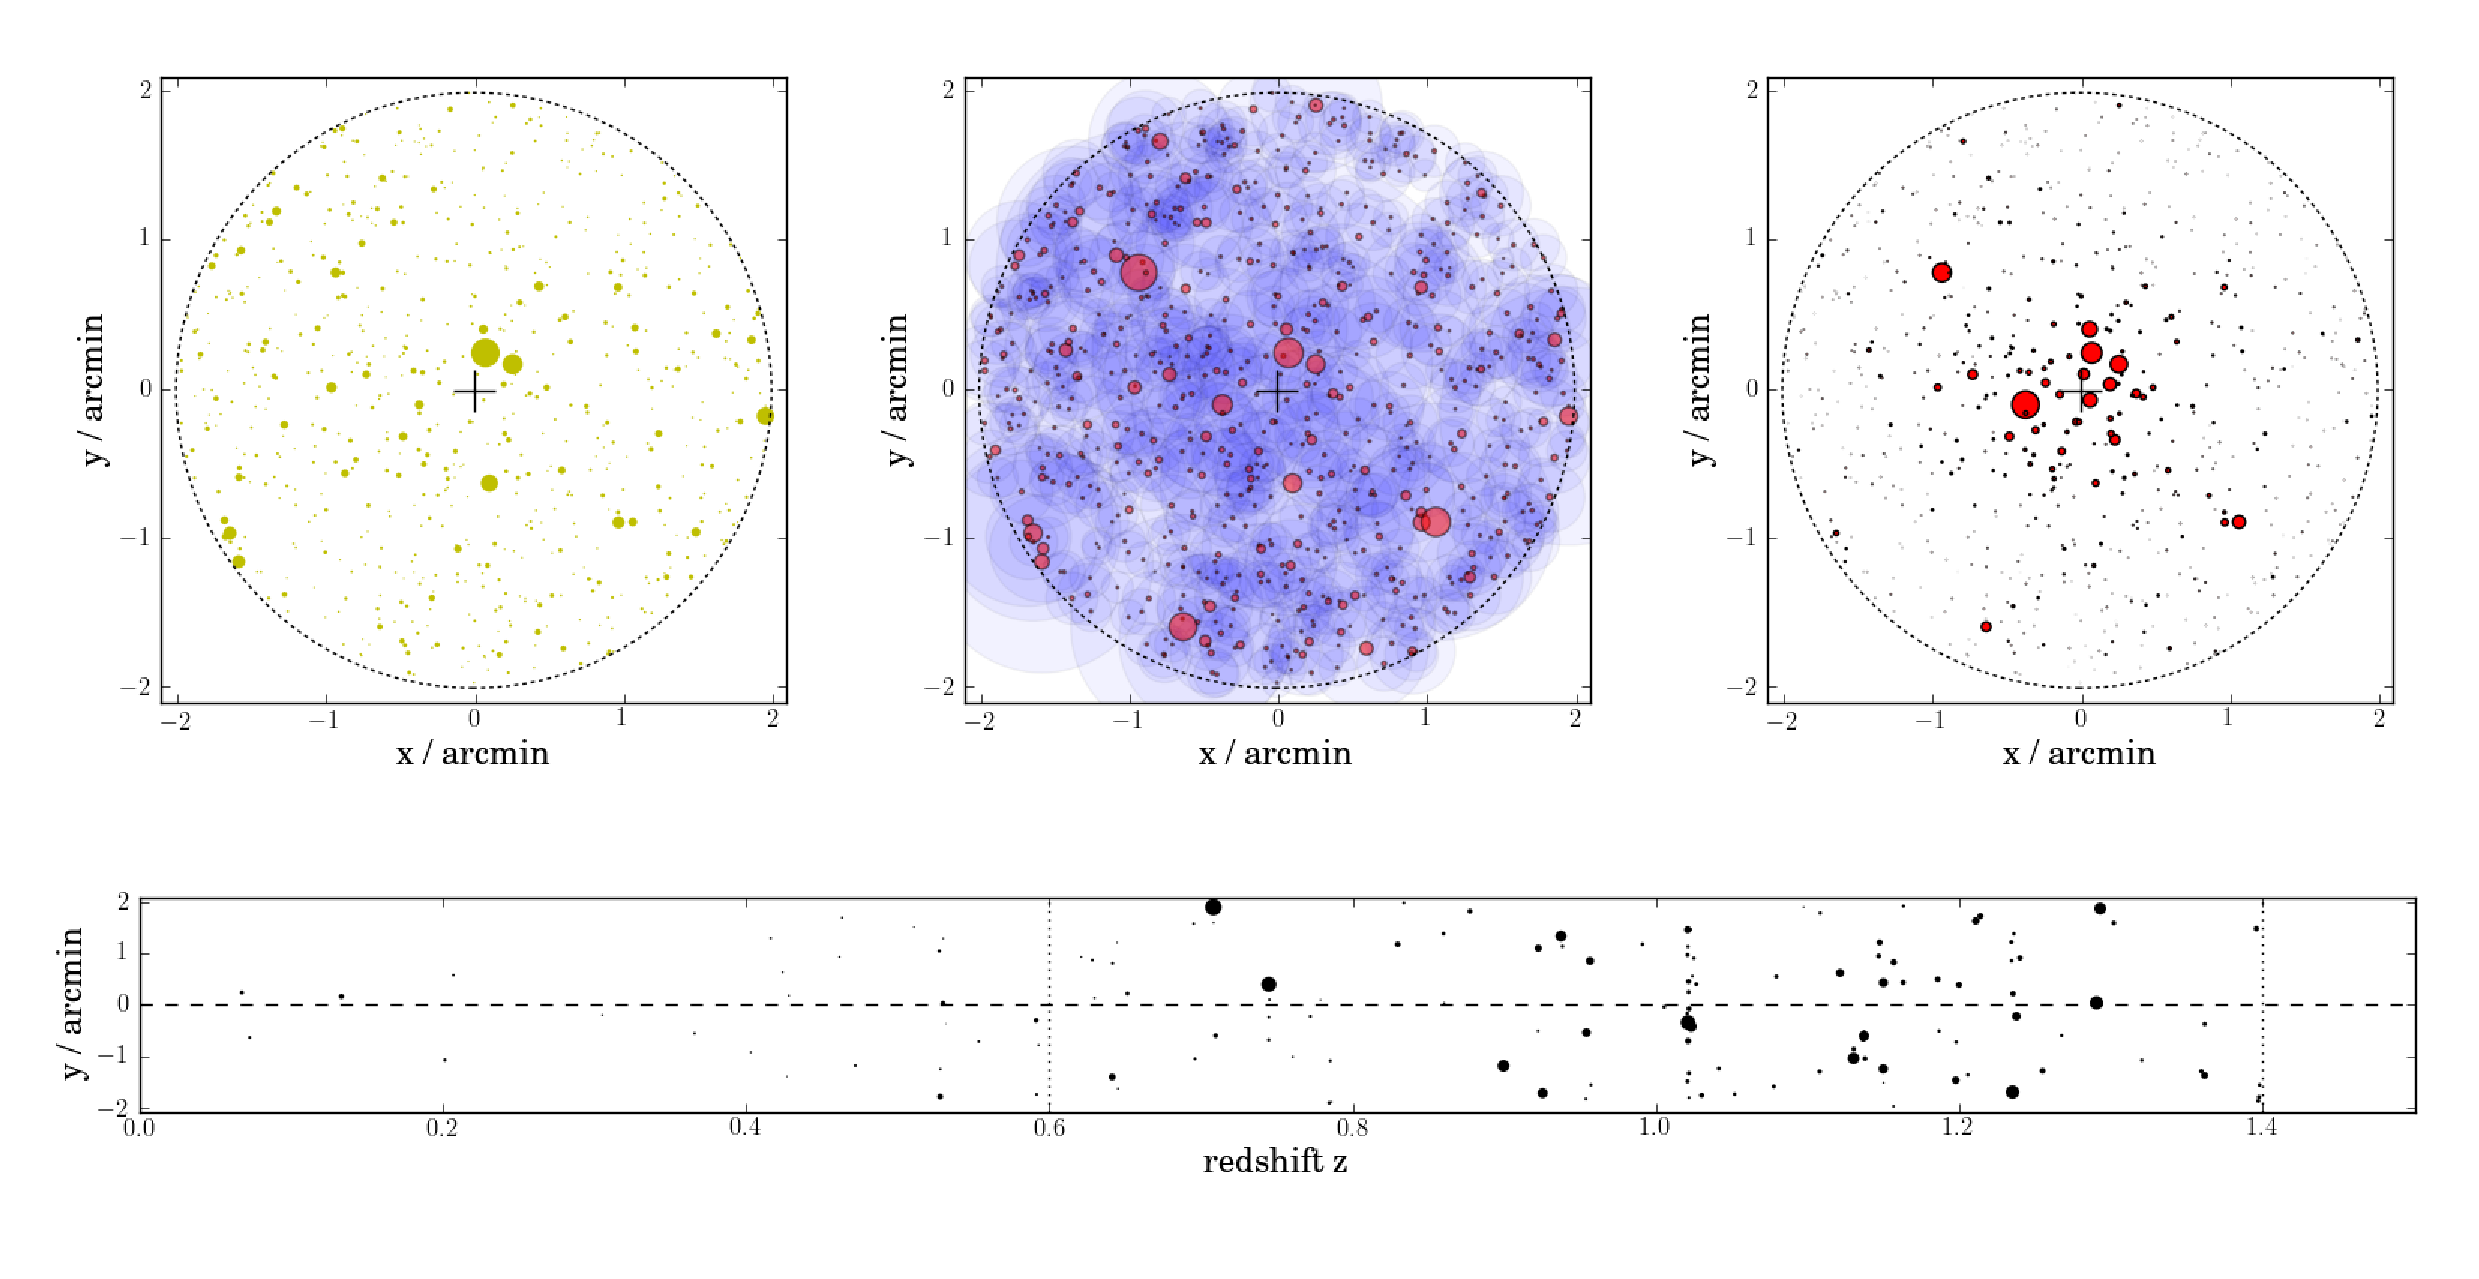
\includegraphics[width=\textwidth]{figs/viewofalightcone.eps}
\caption[magcut]{Four different views of a slightly over-dense \MS line
of sight, with a $\kappax$ of 0.03. 
{\it Top row, left:} The positions of galaxies projected on the sky. The area
of the circles is proportional to observed $i$-band flux; the brightest
object shown has an $i$ magnitude of 17.7. 
{\it Top row, centre:} The angular sizes of halos projected on the sky.
Red and blue regions lie within the NFW scale radius and virial radius
of each halo, respectively. There are essentially no empty lightcones. 
{\it Top row, right:} The individual $\kappax$ contributions of
each halo, assuming a \citet{BMO} truncated NFW 
profile and the \citet{Neto2007}
mass-concentration relation. Comparison of
this panel and the centre panel illustrates the relative importance of
proximity to the line of sight.
{\it Bottom:} A view along the redshift axis, showing only halos with
$|x|<0.3$ arcmin. The area of the points is proportional to each halo's
mass: the most massive halo shown has $1.6\times10^{12}\Msun$. The
optical axis is shown by the dashed line, while the dotted lines mark
the lens and source planes for a B1608-like strong lens.}
\label{fig:lightcone}
\end{figure*}



%%%%%%%%%%%%%%%%%%%%%%%%%%%%%%%%%%%%%%%%%%%%%%%%%%%%%%%%%%%%%%%%%%%%%%%%%%%%%%

\section{Theoretical Background}
\label{sec:theory}

\comments{
Convergence, or Ricci focusing, occurs when a gravitational lens focuses
the rays in a given bundle. This focusing can cause distant objects to
appear brighter, and larger than they would if the lens were removed.
The convergence from an isolated mass sheet is the ratio of the projected surface
mass density ($\Sigma$) \devided by the
critical surface mass density at the redshift of the mass sheet
($\Sigma_{\rm cr}$),
\be
\kappax= \frac {\Sigma}
                              {\Sigma_{\rm cr}(\zd,\zs)}
\ee
where 
\be 
\label{eq:sigcrit} 
\Sigma_{\rm cr}(\zd,\zs) \equiv \frac{c^2 D_{\rm os}}{4 \pi G D_{\rm od} D_{\rm ds}}.
\ee
and the $D$'s are the angular diameter distances between the objects
referred to in the subscripts: o is the observer, d is the deflector and
s is the source. If the surface mass density of the sheet exceeds
$\Sigma_{\rm cr}$, multiple images of the source can occur, otherwise
only one image will be observed, although that image will still be
perturbed relative to the unlensed case.


Strong lensing occurs when a massive object and background source are almost perfectly
aligned along a line of sight. The light from the background source is deflected by the
lens galaxy; this deflection allows multiple images of the background source to form
at stationary points of the time delay function. For an isolated lens, the time delay
function can be calculated from
\be \label{eq:T} 
\Delta t(\bmath{\theta},\bmath{\beta}) = \frac {1}{c} \frac{D_{\rm od} D_{\rm os}}{D_{\rm ds}} (1+z_{\rm d})\, \phi(\bmath{\theta},\bmath{\beta}),
\ee
where $\bmath{\theta}$ is the observed source position, $\bmath{\beta}$ is the 
unlensed source position, $z_{\rm d}$ is the redshift of the lens, $\phi(\bmath{\theta},\bmath{\beta})$ is
the Fermat potential. The Fermat potential is given by
\be \label{eq:FP}
\phi(\bmath{\theta},\bmath{\beta})\equiv \left[\frac{(\bmath{\theta}-\bmath{\beta})^2}{2}-\psi(\bmath{\theta}) \right], 
\ee
where $\psi(\bmath{\theta})$ is the lens potential, derived from the projected dimensionless
surface mass density, $\kappa(\bmath{\theta})$, by 
\be \label{eq:psikappa}
\kappa(\bmath{\theta})=\frac{1}{2}\nabla^2\psi(\bmath{\theta}).
\ee
}


In strong lens systems where the source is time variable, the images do not 
vary simultaneously; the optical path length for each image is different due
to relativistic and geometric effects. The difference in optical path length
causes a time-delay between the light curves of each image.
\citet{FalcoEtal1985} showed that the presence of additional matter (in the
form of a mass-sheet) along the line of sight has no observable effect except
to rescale the time-delays and magnifications. As such, it is necessary to include $\kappax$ in
the lens modelling if cosmological parameters are to be estimated accurately
and precisely from observed time delays \citep{SuyuEtal2010}. 


If there is external convergence present that is not included in the
lens modelling, then the time delay distance -- inferred assuming $\kappax
= 0$ -- will be $(1-\kappax)$ more than the true value of the time-delay distance $\Dt$:
\be 
\label{eq:MassSheet:Dtbias}
\Dt^{\rm{true}}=\frac{\Dt^{{\kappax = 0}}}{1-\kappax}.
\ee

We can hence estimate the true distance {\it only} if we have additional
knowledge of $\kappax$. Since $\kappax$ is typically small the absolute
uncertainty on the estimate of $\kappax$ corresponds to the fractional
uncertainty with which time-delay distances can be \infered.

Dynamical observations of the lens galaxy
can help break the mass-sheet degeneracy by providing an additional
estimate of the lens's mass
\citep[e.g.,][]{KoopmansEtal2003,Koopmans2004,SuyuEtal2010}. This constraint 
is useful in excluding the high convergence tails that are often present in 
PDFs for convergence - we do not include dynamical constraints in our analysis. 

In this paper we restrict ourselves to reconstructing
the line of sight portion of the mass distribution in any given field, {\it our lines of sight do not include a strong lens} which allows us to work in the weak lensing regime.  


The impact of weak-lensing perturbations on strong lensing lines-of-sight is
postponed to further work.

%%%%%%%%%%%%%%%%%%%%%%%%%%%%%%%%%%%%%%%%%%%%%%%%%%%%%%%%%%%%%%%%%%%%%%%%%%%%%%

\section{The Millennium Simulation}
\label{sec:MS}

In order to test the accuracy of our convergence estimates, we need to
know the true convergence for each line of sight. We cannot use  real
lines of sight for this,  but must use simulated lines of sight instead.
In this section we briefly review the Millennium Simulation, the ray
tracing calculations that have been carried out in it, and the mock
galaxy catalogues that have been produced.

The \MS \citep{SpringelEtal2005} is a cosmological N-body simulation of
Dark Matter structures in a cubic region approximately 680~Mpc in
co-moving size, followed from redshift 127 to the present day. With an
approximate halo mass resolution of $2\times10^{10}{\rm M}_{\odot}$
(corresponding approximately to a galaxy with luminosity $0.1L^{*}$), it
provides a detailed prediction for the distribution of dark structures
present in the Universe, under the assumptions of the $\Lambda$CDM model
of hierarchical structure formation, cosmological densities as given at
the end of \Sref{sec:intro}, and $\sigma_8 = 0.9$.
Galaxy properties,
such as stellar masses, luminosities and colours, were assigned to the
simulated halos according to a semi-analytic model for galaxy formation
\citep{DeLucia+Blaizot2007}: the resulting predictions for the galaxy
luminosity function and correlation function match the observational
data very well.

% % % % % % % % % % % % % % % % % % % % % % % % % % % % % % % % % % % % % % % 

\subsection{Convergence from Ray Tracing}
\label{sec:MS:raytracing}

\citet{HilbertEtal2009} calculated the lensing convergence using the
``lightcone'' dark matter only  output of the \MS, providing 1.7 degree
square  mock sky maps of this quantity. In this process, the dark matter
density from the simulation was projected onto a set of lens planes at
discrete redshifts, adaptively gridded and smoothed, and then the second
derivatives of the  lensing potential required for the components of the
magnification matrix were computed using a multiple lens plane ray tracing
algorithm. The first order approximation to this algorithm \citep[equation 17
of][]{HilbertEtal2009} gives the total convergence at a given sky
position~$\bmath{\theta}$ as the simple summation of the surface density in
each lens plane, weighted by the inverse critical surface density $\Sigma_{\rm
cr}$ for that plane's redshift:
\be
\kappax(\bmath{\theta}) = \sum_i \frac{\Sigma_i(\bmath{\theta})}
                                     {\Sigma_{\rm cr}(z_i,\zs)}.
\ee
\citet{HilbertEtal2009} found that this approximation is accurate to a percent level
in $\kappax$, even on 30 arcsecond scales. This accuracy sufficient for our analysis, but 
the approximation may need re-visiting in future work.

To define a test line of sight, we draw a random sky position from
within the convergence maps, bi-linearly interpolate between the pixels
of the map, and store the result as the ``true'' convergence for that
line of sight, $\kappax^{\rm true}$. 


\new{The adaptive smoothing of the matter in the \MS results in a spatial resolution of $\sim 5\,\text{kpc}$ comoving in the densest regions, and $\sim10\,\text{kpc}$ on average. This resolution is sufficient to capture most of the variance in the convergence \citep{TakahashiEtal2011}. Moreover, we seek to estimate the component of the convergence that is smooth on the angular scales of typical strong galaxy-scale lens systems ($\sim 1\,\text{arcsec}$). Any variations of the external convergence on smaller scales can be directly recovered from the resulting image distortions in the lens modelling.}


\comment{PJM: This means our sightlines are not typical of strong lenses, because they
don't include the local overdense region typically found near massive lens
galaxies. Our lines of sight have typical mass distributions for a lens line
of sight {\it after excision of the lens plane}. I have tried to explain
this above.}

% % % % % % % % % % % % % % % % % % % % % % % % % % % % % % % % % % % % % % % 

\subsection{Mock Photometric Galaxy Catalogues}
\label{sec:MS:mocks}

We construct mock photometric galaxy catalogues by selecting all \MS galaxies
within a circular aperture of a given angular radius centred on each randomly
selected line of sight position, with apparent $i$-band magnitude brighter
than a given limit. The parent catalogue, from \citet{HilbertEtal2011},
contains galaxy positions and magnitudes, all of which include lensing effects
(deflections and magnifications). We also have access to the underlying galaxy
halo masses and redshifts, which we will use to calibrate the reconstruction,
and also to explore any sources of bias and scatter. Since the ``true''
convergence is that of only the dark matter, we focus on reconstructing the
dark matter halos alone. Our model for doing this is outlined in the next
section. 

%%%%%%%%%%%%%%%%%%%%%%%%%%%%%%%%%%%%%%%%%%%%%%%%%%%%%%%%%%%%%%%%%%%%%%%%%%%%%%

\section{Estimating Convergence: The Halo Model Approximation}
\label{sec:model}

We require a method for estimating the convergence at any point on the sky,
given a catalogue of observed galaxy properties such as positions,
brightnesses, colours, and possibly stellar masses and redshifts, for every
galaxy in the field of the lens, down to some magnitude limit. Since we cannot
observe the surface mass density of each halo directly, we need some way of
estimating the mass of each halo in the catalogue, so that we can compute its
contribution to the total $\kappax$ along the line of sight \citep[as in
\eg][]{GunnarssonEtal2006,KarpenkaEtal2012}.  This mass
assignment recipe will be uncertain, and also incomplete, but it can be
calibrated with cosmological simulations, which represent a significant
additional source of information to what is present in the data.

Transforming an observed photometric galaxy catalogue into a  catalogue of
halo masses, positions, and redshifts will enable us to attempt a
reconstruction of the convergence induced by every halo near a line of sight. 
We also need to account for the convergence due to dark structures and the
divergence due to voids; we do not model voids or dark structures, but their
effects are included statistically by calibrating the convergence in
halos, $\kappah$, against the ray-traced convergence, $\kappax$, for \MS lines
of sight.


% % % % % % % % % % % % % % % % % % % % % % % % % % % % % % % % % % % % % % % 

\subsection{Halos}
\label{sec:model:halos}

Cosmological dark matter simulations have shown that dark matter
halos are reasonably well-approximated by NFW profiles 
\citep{NFW}. We assume each halo to have a spherical mass distribution with 
density given by
\be\label{eq:rhonfw}
\rho(r) = 
\frac{\rho_0}{\left(r/r_{s}\right)
\left(1+r/r_{s}\right)^{2}}.
\ee
Here, $r_{s}$ is a characteristic scale 
radius of the cluster, representing the point where
the density slope transitions from $r^{-1}$ to $r^{-3}$. This radius is
related to the virial radius of the halo by $r_{s}~=~r_{200}/c$, where $c$ is
the concentration parameter, which can be estimated from the halo's mass,
using a mass--concentration relation. Typically more massive halos are less
concentrated, but there is some scatter; we use the relation of
\citet{Neto2007} to estimate $c$ from the mass enclosed within $r_{200}$,
which we denote as $M_{200}$. We find our results do not change if the
\citet{MaccioEtal2008} mass--concentration relation is used instead. 

If one integrates the density profile of an NFW profile out to infinite
radius, the total mass diverges. Similarly, if the universe is
homogeneously populated with NFW halos, the projected surface mass along
any line of sight will also be divergent.\footnote{At large radius,
$\Sigma_{\rm nfw} \propto R^{-2}$, but the differential number of halos
centred within an annulus of width $\dee R$ is given by $\dee N_{\rm
annulus} \propto R \dee R$, so  $\Sigma_{\rm total} \propto
\int_{0}^{\infty} R^{-1} \dee R$, which diverges logarithmically} Since
infinite mass is unphysical, the profile must be truncated at some
point. Several truncation profiles have been suggested
\citep[e.g][]{BMO}, but beyond several virial radii, the amount of
matter associated with a halo is likely to be low. In this work we
assume the truncated NFW profile
\be\label{eq:bmoprofile}
\rho(r) = 
\frac{\rho_{\rm NFW} (r)}{1+\left(r/r_{t}\right)^2},
\ee
which is the same as the NFW profile in the limit that the truncation
radius, $r_t$ goes to infinity; the shear and convergence from such a
profile are derived in \citet{BMO}.
 We use a truncation radius of five times
the virial radius, but our results are robust for any choice of $r_t>2
\times r_{200}$. 

Many studies have shown that galaxies have total mass density profiles that
are approximately isothermal in their inner regions
\citep[\eg][]{AugerEtal2010} due to the more concentrated stellar mass
component.
This has been confirmed by galaxy-galaxy weak lensing measurements 
\citep[\eg][]{Mandelbaum,GavazziEtal2007}. We note that the two halo term that
dominates the galaxy-galaxy lensing signal at large radii is explicitly taken
into account in our model, where every galaxy is assigned a dark matter halo.
At large radii an NFW-like profile is probably appropriate, but may not be
correct when a halo is very close to the line of sight.


Each halo in our catalogue contributes to
the line of sight convergence by
\be
\label{eq:kappai}
\kappa_i =\Sigma_{i}/\Sigma_{\mathrm{cr}}(z_i,\zs),
\ee
where $\Sigma_{\mathrm{cr}}(z_i,\zs)$ is the critical surface density \comments{was defined in \Eref{eq:sigcrit}}.
Following the first order approximation of \citet{HilbertEtal2009}
outlined in \Sref{sec:MS} above, we compute 
the total convergence from all the halos along the line
of sight using
\be 
\label{eq:kappasummu}
\kappah = \sum_{i} \kappa_i.
\ee

To estimate a halo's contribution to $\kappah$ we must first know the
halo's mass \new{and position. The stellar mass
and host halo are not necessarily concentric, especially for central
galaxies of giant clusters, but our reconstruction assumes the dark matter halo is centred on
the visible galaxy.} For the lines of sight of the \MS, halo masses are
known, but for  real lines of sight the halo masses have to be \infered
from whatever data are available. 
In this work we investigate the use of the empirical stellar mass --
halo mass relation for this purpose. The primary advantage of this
approach is that it is a simple, ``one size fits all'' relation that can
be applied regardless of the stellar mass observed. We discuss
additional observables that could be used to improve the precision of
the halo mass inference in \Sref{sec:discuss} below. 

We use the relation of \citet{BehrooziEtal2010} to infer halo masses
from stellar masses; the details of this \proceedure are outlined in 
\Aref{appendix:MSMH}. Given an uncertain stellar mass and redshift for
each galaxy in the  catalogue, we draw a sample halo mass from the PDF
that describes this uncertainty (\Eref{eq:mhalo-mstar}) and use
\Eref{eq:kappai} to compute its contribution to the convergence,
$\kappa_i$; this can be done for all the halos along a specific line of sight
and summed to give a sample value of $\kappah$;  repeatedly applying
this \proceedure allows us to build up a histogram of $\kappah$ values
consistent with the data, and hence characterize $\pr(\kappah|\data)$. 

This PDF contains a hidden assumption of an uninformative prior PDF for
$\kappah$ -- in the case of infinitely poorly measured stellar masses and
redshifts, $\pr(\kappah|\data)$ will have very long tails corresponding to
very over-dense lines of sight that we do not believe exist. The resolution of this
is to divide out the effective prior PDF that was applied during the halo mass
estimation process (which is broad, and hence close to uniform), and apply an
additional prior on $\kappah$, given by the global underlying $\kappah$
distribution from the simulation. In the limiting  case of very poor
photometric data, $\pr(\kappah|\data)$ then defaults to this distribution, as
required.

% \todo{All}{Discuss this. It ties us to the simulation, but only weakly. Is the
% argument about poor data valid? Tom?}

% TEC: yes it's valid. It only really ties us to the halo mass function of the
% simulation. It's probably tied at the same level as the "global P(\kappa) as
% derived from Stefan's ray-tracing"


% % % % % % % % % % % % % % % % % % % % % % % % % % % % % % % % % % % % % % % 

\subsection{Accounting for voids, filaments and other dark structures}
\label{sec:model:voids}

Our halo model accounts for the convergence contribution of density
perturbations that can be associated with light. Filaments and dark
substructures contribute additional convergence, while voids contribute a
divergence; these structures must be included to produce an unbiased estimate
of $\kappax$. In particular, neglecting voids would lead to a heavily biased
estimate of $\kappax$, since the halo model's $\kappah$ can only be positive.
In principle the absence of galaxies implies something about the presence of a
void, but we do not currently attempt to use this information. In general, it
is difficult to account for the unseen mass, since we do not have a good model
for its density structure.

The solution we present here is to calibrate the relationship between the halo
convergence $\kappah$ and the overall convergence $\kappax$ (as would be
calculated by ray tracing through the full density field)  using the
simulations themselves. The halo modelling procedure outlined in
\Sref{sec:model:halos} allows  us to estimate  the convergence due to halos
given observations of  mass, redshift and position,
$\pr(\kappah|\data)$, but what we are interested in is the total
convergence along the line of sight $\pr(\kappax|\data)$. We can obtain
this by considering the expression: 
\begin{equation} 
\Pr(\kappax|\data) = 
   \int \dee\kappah  \Pr(\kappax|\kappah,\data) \Pr(\kappah|\data)
   \label{eq:kappaconv}
\end{equation} 
The first term in the integrand relates the convergence due to model halos,
$\kappah$, to the true convergence, $\kappax$. This conditional distribution
can be constructed from the \MS catalogues, by computing
$\kappah$ from the true halo masses and redshifts 
along each selected line of sight, and then
accumulating $\kappah$, $\kappax$ pairs
for a large number of such sightlines. 
For any given line of sight we can then estimate
$\pr(\kappah|\data)$ as described above, and then multiply it by
$\Pr(\kappax|\kappah)$ and integrate out the intermediate parameter
$\kappah$. 

\phil{However, if the conversion between stellar mass and halo mass is very
uncertain, $\pr(\kappah|\data)$ is shifted relative to what it would
have been given perfect knowledge of the halo masses.  This is because the
conversion from stellar mass to halo mass and into $\kappah$ is highly
asymmetric: a long tail of high halo masses gives rise to a tendency to
overestimate $\kappah$. If this shift is ignored, the resulting
$\Pr(\kappax|\data)$ will be systematically biased towards high values of
$\kappax$. Instead, we need the  distribution of $\kappax$ from all
calibration lines of sight that have a $\pr(\kappah|\data)$ that is identical
to the $\pr(\kappah|\data)$ for the real line of sight {\it given the same
data quality}; however, we found this approach unfeasible  given our finite
number of calibration lines of sight. A working compromise is to use 
the median of the $\pr(\kappah|\data)$ distributions in the calibration.}

We  take a large number of
calibration lines of sight from the \MS catalogues and generate a mock
stellar mass catalogue for each one. We then reconstruct each lightcone in the
same way as we would an observed field,
estimate $\pr(\kappah|\data)$, and extract its median. Accumulating
these median values $\kappah^{\rm med}$ and 
their corresponding true values of $\kappax$, we can form the 
conditional distribution $\pr(\kappax|\kappah^{\rm med})$. 
Then, to infer $\kappax$ from an observed photometric catalogue, we 
estimate $\pr(\kappah|\data)$ 
using the halo model, compute the median value 
$\kappa_{\rm h,obs}^{\rm med}$, and then use a modified
version of 
\Eref{eq:kappaconv} to infer $\kappax$: 
\bea
\Pr(\kappax|\kappah^{\rm med},\data) &=& \int \dee\kappah^{\rm med} 
   \Pr(\kappax|\kappah^{\rm med},\data) \Pr(\kappah^{\rm med}|\data) \notag \\
\label{eq:calkappaconv}   
\eea
\phil{This integral is trivial, since $\Pr(\kappah^{\rm med}|\data)$ is
a delta function centred on the median of the inferred PDF for $\kappah$.
However,}
because we only have a finite number of calibration lines of sight, we use all
calibration lines of sight with $\kappa_{\rm h,cal}^{\rm med} =
\kappah^{\rm med}\pm0.003$ to form $\Pr(\kappax|\kappah^{\rm
med},\data)$.
\comments{, with each calibration sightline weighted equally. PJM: why is
this? Surely one should weight by the value of the Gaussian function implied
by that ``$\pm 0.003$''?}

This procedure of reducing the full PDF for $\kappah$ to its median increases
the importance of the realism of the simulation: the simulation needs to be as
similar as possible to the real universe or there is a possibility of
systematic errors. Conversely, making use of all the information
in the photometric catalogue yields $\kappax$ estimates of increased
precision.

%%%%%%%%%%%%%%%%%%%%%%%%%%%%%%%%%%%%%%%%%%%%%%%%%%%%%%%%%%%%%%%%%%%%%%%%%%%%%%

\section{Results: Perfect Halo Data}
\label{sec:knownMh+z} 

We now put the reconstruction \proceedure outlined above into practice, first
inferring $\kappax$ from $\kappah$ in the case of hypothetical galaxy
catalogues with noiseless redshifts and halo masses. The reason for doing this
is to check the validity of the calibration process, and then also to 
investigate the primary sources of the convergence. It will also provide us
with a measure of the intrinsic uncertainty introduced by our assumptions of
all illuminated halos being spherically-symmetric truncated NFW halos following the
Neto et al concentration--mass relation \new{and of visible galaxies being concentric with their host halos}.

% % % % % % % % % % % % % % % % % % % % % % % % % % % % % % % % % % % % % % % 

\subsection{How is $\kappah$ related to $\kappax$?}

\Fref{fig:jointkh-k} shows the conditional distribution of $\kappax$ given 
$\kappah$, derived from $10^5$ randomly selected \MS lines of sight
and assuming noise-free halo masses and redshifts. 
\phil{In this case, $\pr(\kappah|\data)$ is almost a delta function since the only uncertainty is halo
concentration, which has minimal effect on $\pr(\kappah|\data)$.  
}
% In this case, the PDF : we can read
% off  $\pr(\kappax|\data)$ just by taking a thin vertical slice through this 
% distribution. 
% Note that the joint PDF plotted in this figure is the product
% of  the conditional distribution that we need for calibration, and also the
% prior PDF for $\kappah$ that we need to ensure that the global distribution of
% $\kappah$ values is defaulted to in the case of poor observational data. 
At fixed $\kappah$ we find in \Fref{fig:jointkh-k} that the scatter in 
$\kappax$
grows with $\kappah$; our reconstruction is better at reproducing under-dense
lines of sight than over-dense lines of sight. The effect of ignoring voids
and the smooth mass component is evident in this plot: $\kappah$ is
significantly higher than $\kappax$, at any given $\kappax$ value. 
\phil{Conditioning on $\kappah$ gives a PDF for
$\kappax$ centred at the correct place, by construction.}

%%%%%%%%%%%%%%%%%%%%%%%%%%%%%%%%%%%%
\begin{figure}
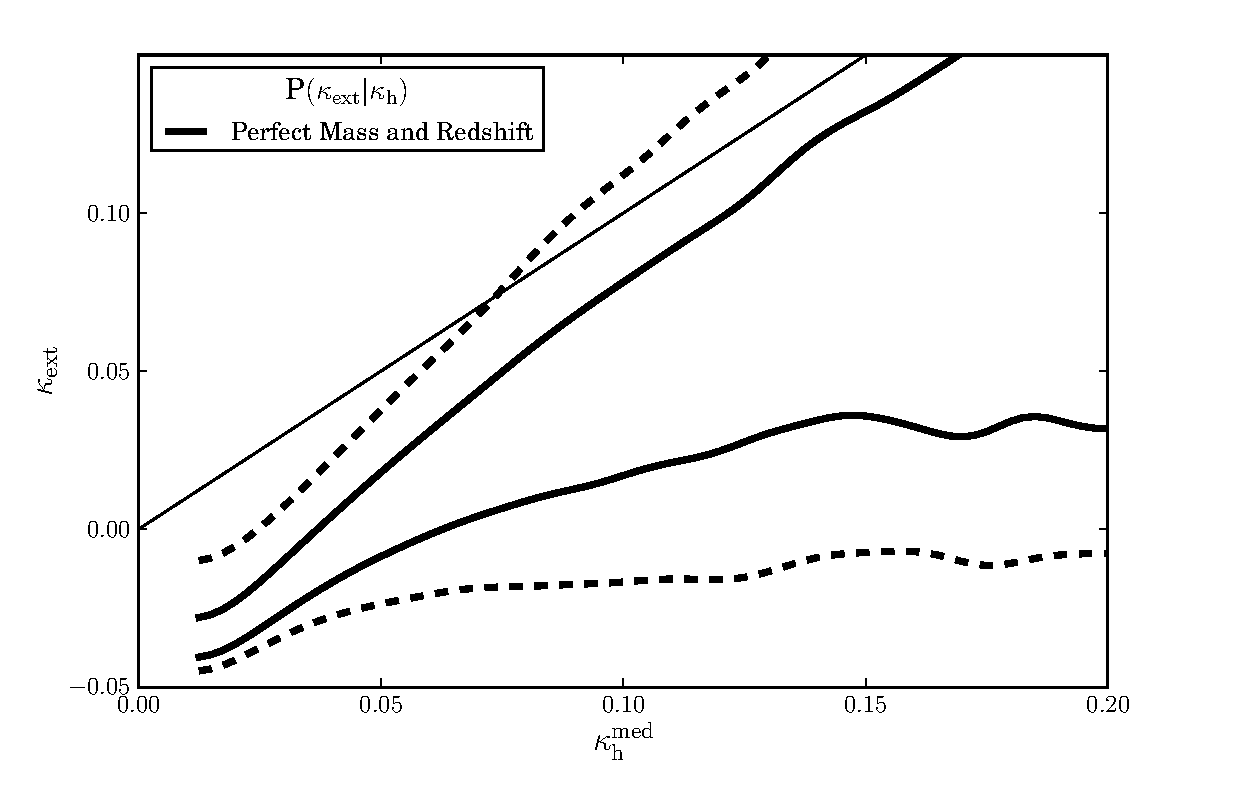
\includegraphics[width=\columnwidth]{figs/cornerplot.eps}
\caption[Biased?]{The conditional distribution of 
$\kappax$ given $\kappah$, in the case where  
we have perfect knowledge of halo mass and redshift.
$10^5$ reconstructed lines of
sight were used to make this plot. 
Solid (dashed) lines enclose 68\% (95\%) of the conditional probability.
$\kappah$ traces $\kappax$, but with a positive offset which arises from
$\kappah$ not accounting for any voids or dark structures.
At fixed $\kappah$ the scatter in $\kappax$ grows rapidly with $\kappah$.
\tom{The thin diagonal line follows $\kappax=\kappah$.}}
\label{fig:jointkh-k}
\end{figure}
%%%%%%%%%%%%%%%%%%%%%%%%%%%%%%%%%%%%


% % % % % % % % % % % % % % % % % % % % % % % % % % % % % % % % % % % % % % % 

\subsection{How accurate is the $\kappah - \kappax$ calibration?}

%%%%%%%%%%%%%%%%%%%%%%%%%%%%%%%%%%%%
\begin{figure}
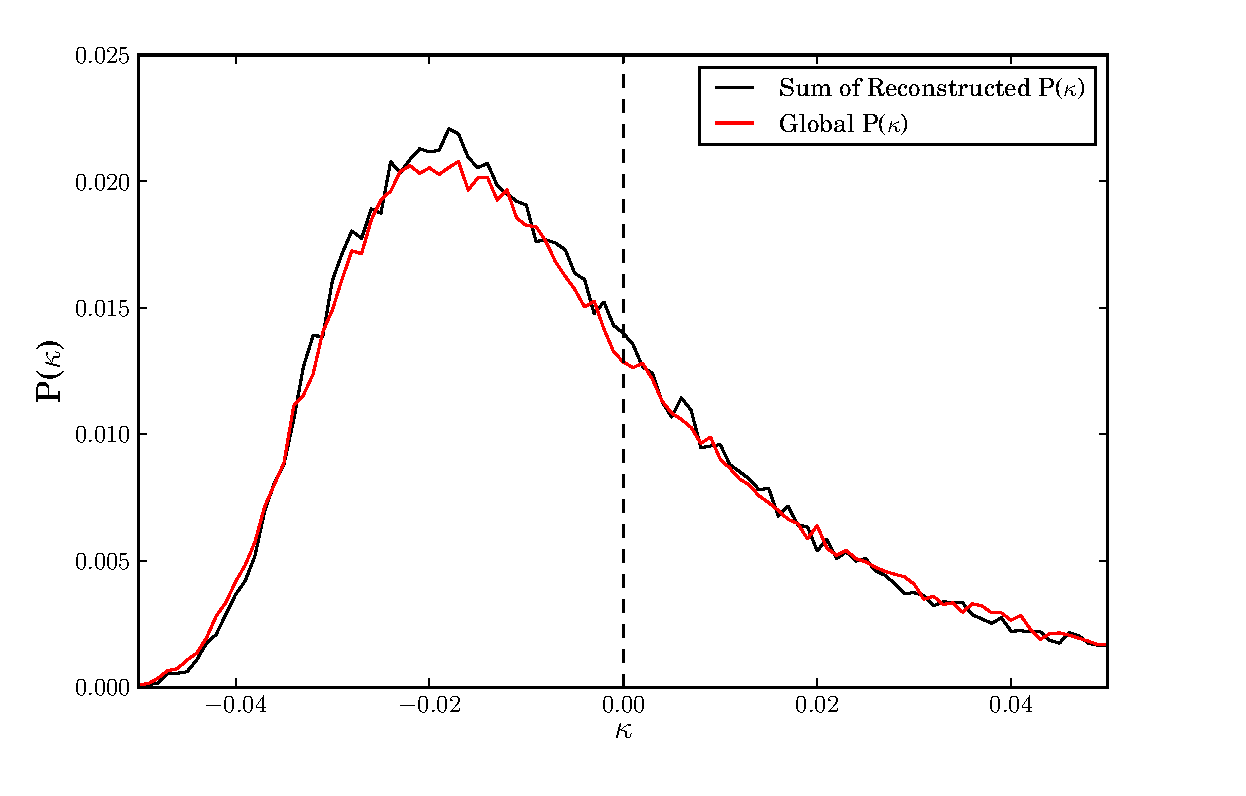
\includegraphics[width=\columnwidth]{figs/globaldist.eps}
\caption[magcut]{Recovering the global $\pr(\kappax)$ (shown in red). The
black curve shows a histogram of  inferred  $\kappax$ values from $10^{5}$
reconstructed lines of sight.  The reconstructions were performed given
perfect knowledge of halo mass and redshift -- in this case the reconstruction
recovers the correct convergence.}
\label{fig:globaldist}
\end{figure}
%%%%%%%%%%%%%%%%%%%%%%%%%%%%%%%%%%%%

%%%%%%%%%%%%%%%%%%%%%%%%%%%%%%%%%%%%
\begin{figure*}
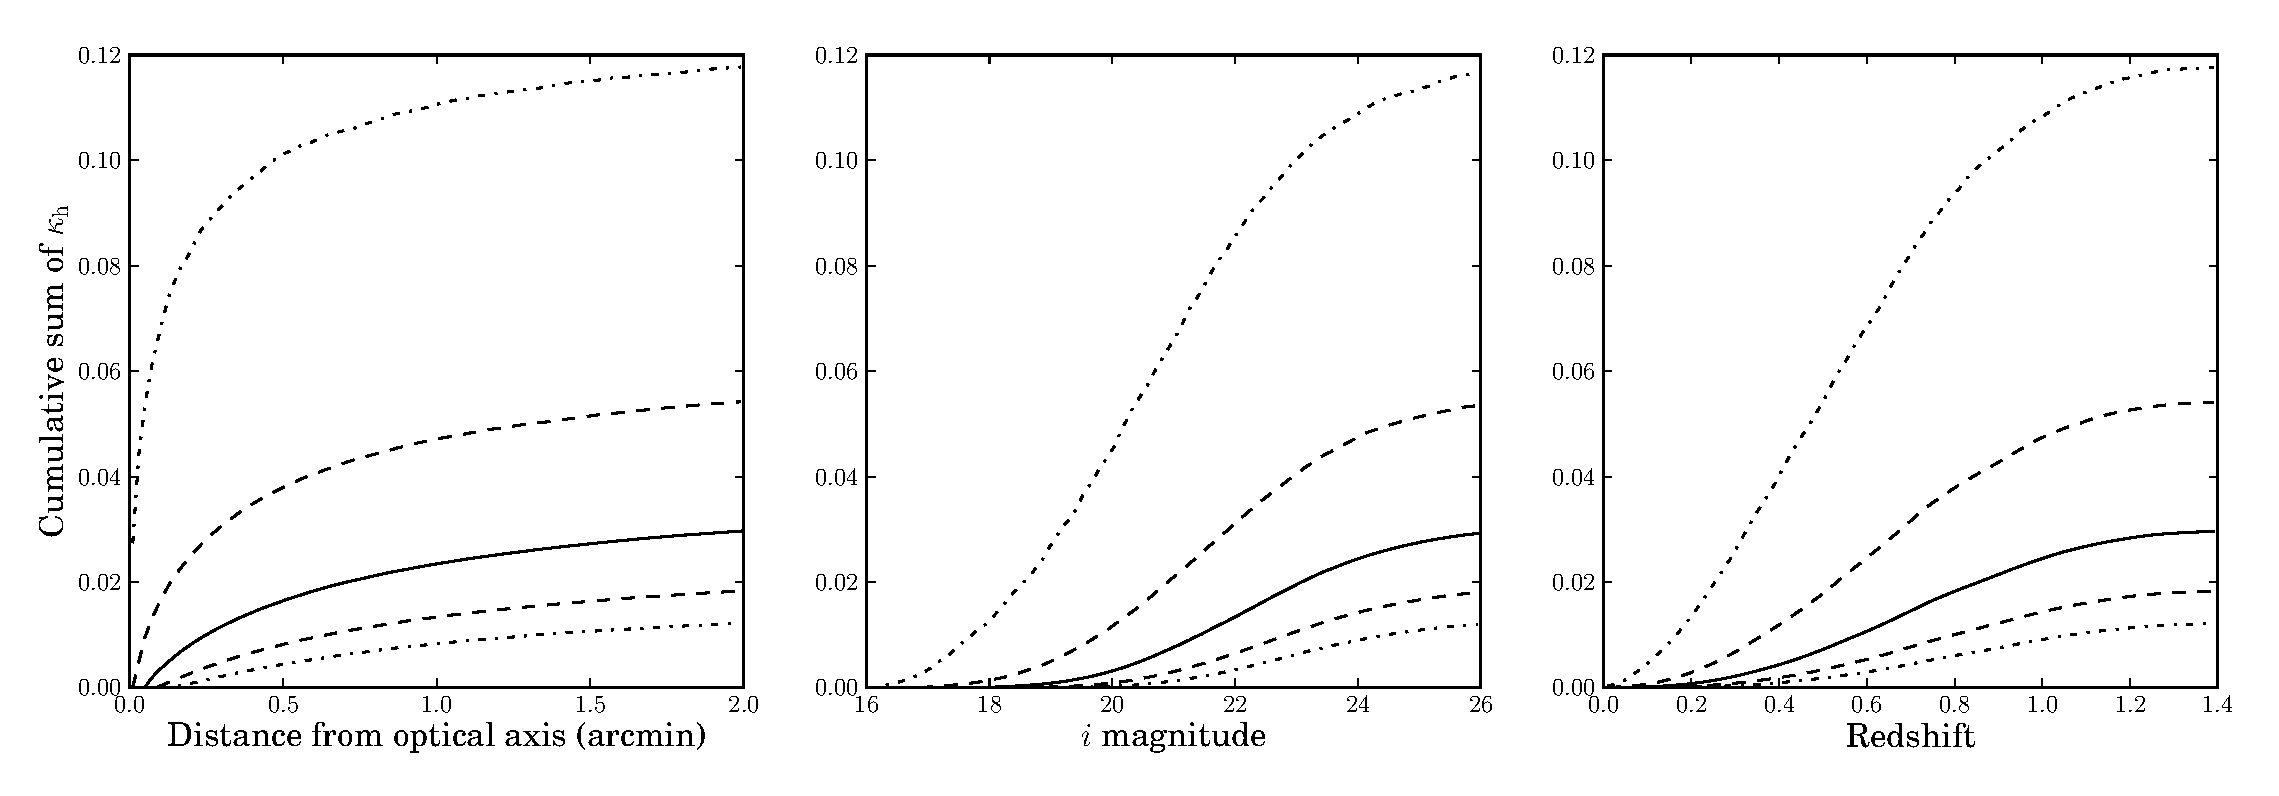
\includegraphics[width=\textwidth]{figs/where_is_the_kappa.eps}
\caption[magcut]{Which objects dominate the external convergence for a line of
sight? From left to right, the three figures show the cumulative contribution
to the total convergence from individual halos ($\kappah$) as a function of
1) distance from the line of sight, 2) magnitude and 3) redshift.   In each
panel, the solid line is the median cumulative contribution over a large
sample of lines of sight, while dashed and dot-dashed show the ranges enclosing 68
and 95 percent of the lines of sight respectively. The source is at redshift 1.4.}
\label{fig:where}
\end{figure*}
%%%%%%%%%%%%%%%%%%%%%%%%%%%%%%%%%%%%

Let us define the ``bias'' of the reconstruction of a given line of sight as
the difference between the expectation value of $\kappax$ over its posterior
PDF $\pr(\kappax|\data)$ and the known true value $\kappax^{\mathrm{true}}$.
Let us also define the ``width,'' $\sigma_{\kappa}$, to be half the width of
the interval containing the central $68\%$ of the posterior probability
$\pr(\kappax|\data)$. 

In an ensemble of $10^{5}$ reconstructed lines of sight, we find the mean bias
to be $-1\times 10^{-5}$, and the mean width to be 0.01. This is
1.8 times smaller than the width of the global $\pr(\kappax)$.  We find that
our inferred $\kappax$ PDFs are consistent with the global $\kappax$
distribution; \Fref{fig:globaldist} shows that sampling from the
$\pr(\kappax|\data)$ inferred from reconstructions of  $10^{5}$ lines of
sight  produces a distribution of $\kappax$ values over the sky nearly identical to
the global $\pr(\kappax)$. Given perfect knowledge of halo mass and redshift
then, the calibration \proceedure provides an unbiased estimate of $\kappax$
that is $1.8$ times more precise than using the global $\pr(\kappax)$. 
\phil{This is the maximum precision we can obtain using the current calibrated
halo model.}

% % % % % % % % % % % % % % % % % % % % % % % % % % % % % % % % % % % % % % % 

\subsection{Which halos dominate the $\kappah$ distribution?}

Before investigating the impact of imperfect knowledge of halo
mass and redshift, we investigate the uncertainties induced by limits on the
magnitude of the observed galaxy sample, and on the field of view. The halos
in our catalogue are populated by galaxies and given magnitudes according to
the semi-analytic model of \citet{DeLucia+Blaizot2007}: by applying magnitude
cuts to our catalogue, we can investigate the amount of scatter caused by
unobserved halos. 

\Fref{fig:where} shows the cumulative contribution to $\kappah$ as a function
of projected distance from the line of sight, magnitude and redshift. We find
that most of the convergence comes from halos close to the line of sight. 
Over half of the  convergence typically comes from halos within 30 arcseconds
of the line of sight; by 2 arcminutes, this fraction is 85\%. The contribution
from halos beyond 2 arcminutes is relatively constant at a contribution of
0.008$\pm$0.003. We find that ignoring halos beyond 2 arcminutes has no effect
on the precision of the reconstruction; this is shown in \Fref{fig:radcut}. As
a function of magnitude, we find that $\kappah$ is dominated by objects with
magnitudes between $i=18$ and $i=24$. Objects brighter than $i=18$ are either
too rare, or too close to the observer, to make a significant contribution to
the convergence. Objects fainter than $i=24$ are too small to be important,
unless they are extremely close to the line of sight; we find that
including halos fainter than $i=24$ does not improve the reconstruction. 
\Fref{fig:magcut} shows the scatter on $\kappah-\kappax$ (where $\kappah$ is
shifted so that its mean is zero, \phil{to emulate the effect of the eventual
calibration}) as a function of reconstruction magnitude limit. We do not
expect a deeper survey to decrease the size of the uncertainty in mapping
$\kappah$ onto $\kappax$. Halos at all redshifts out to the source redshift
(1.4 in this work. The redshift of the source in B1608+656) contribute to the convergence, but the largest contribution comes
from halos with $z \sim z_{\rm source}/2$.

%%%%%%%%%%%%%%%%%%%%%%%%%%%%%
\begin{figure}
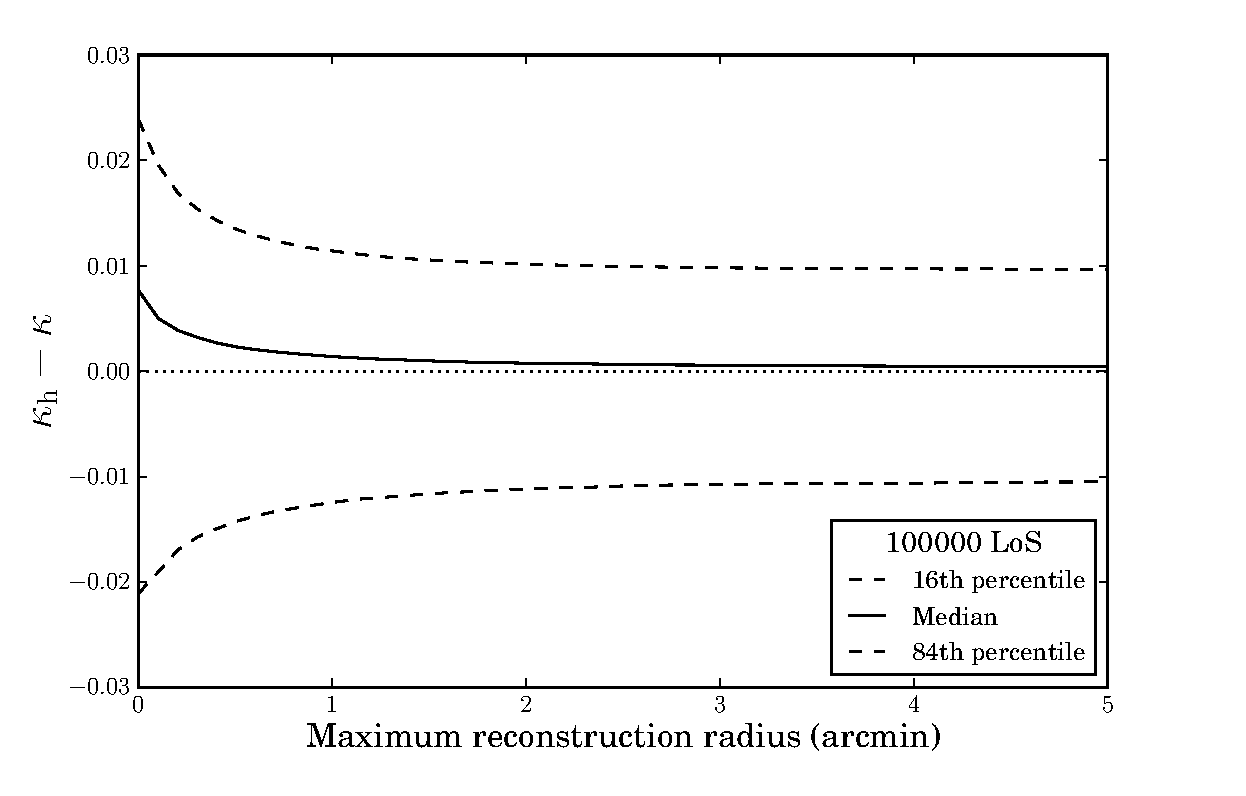
\includegraphics[width=\columnwidth]{figs/radius_scatter.eps}
\caption[magcut]{The 16, 50 and 84th percentiles of $\kappah$ minus
$\kappax$ as a function of the limiting radius of the halo
reconstruction. $\kappah$ has been shifted such that
$\left\langle\kappah\right\rangle=0$ \phil{to emulate the effect of the
eventual calibration}. 
The majority of the constraining power
comes from reconstructing halos within 2~arcmin of the line of sight.}
\label{fig:radcut}
\end{figure}
%%%%%%%%%%%%%%%%%%%%%%%%%%%%%

%%%%%%%%%%%%%%%%%%%%%%%%%%%%%
\begin{figure}
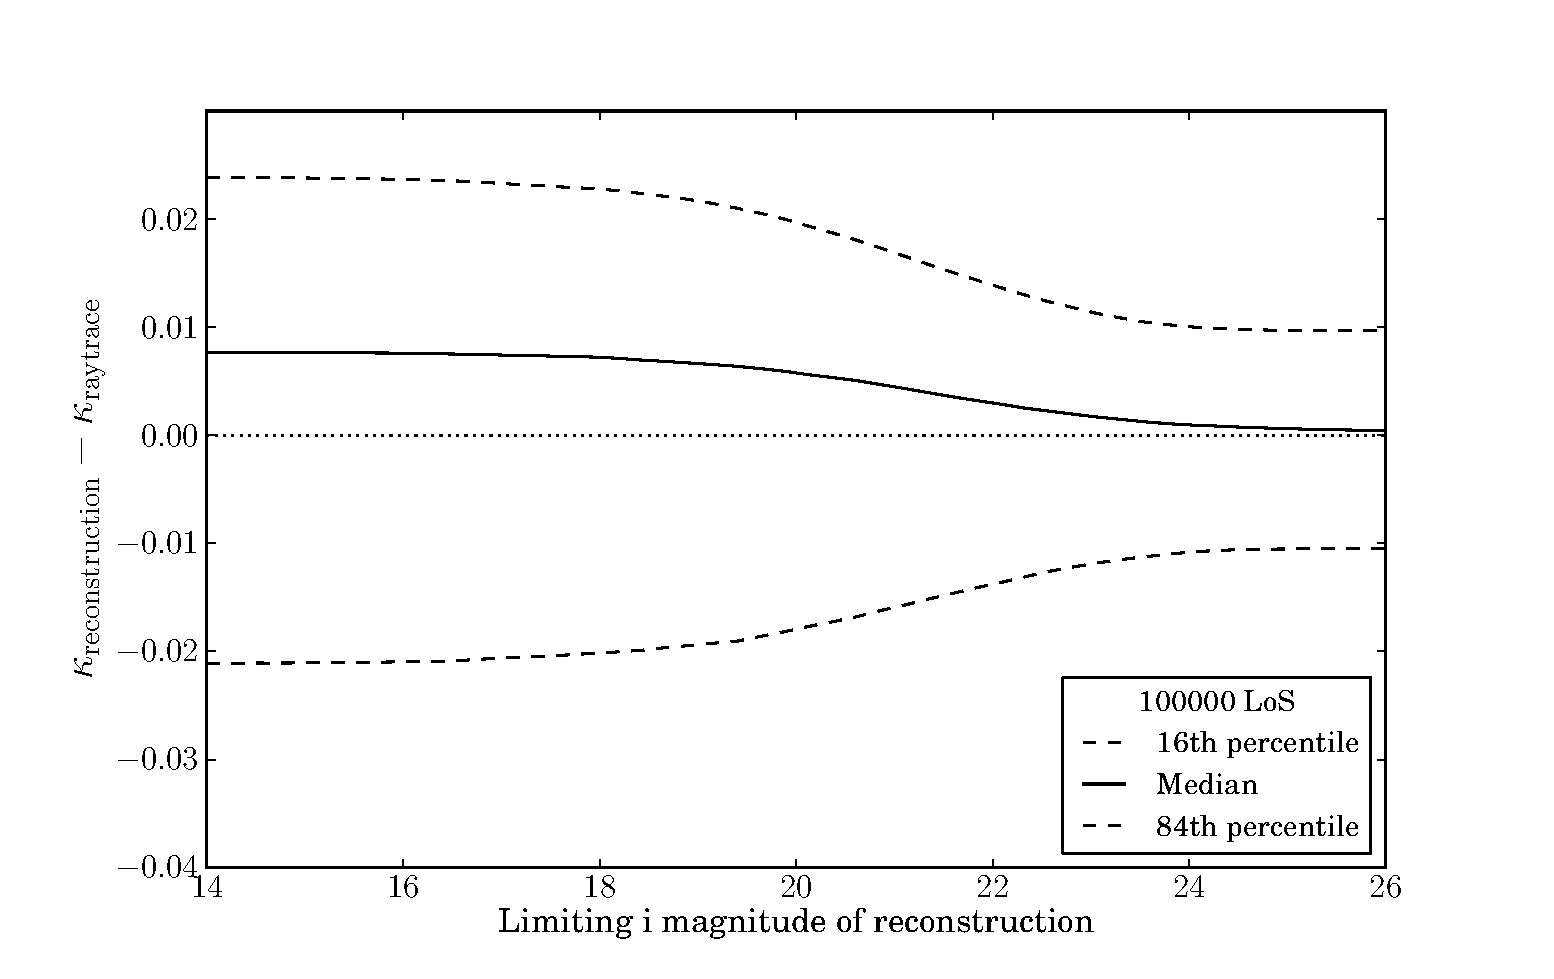
\includegraphics[width=\columnwidth]{figs/mag_scatter.eps}
\caption[magcut]{The 16, 50 and 84th percentiles of $\kappah$ minus
$\kappax$ as a function of the limiting $i$ band depth of the halo
reconstruction. $\kappah$ has been shifted such that
$\left\langle\kappah\right\rangle=0$ \phil{to emulate the effect of the
eventual calibration}. The majority of the constraining power
comes from reconstructing halos with magnitudes between $18<i<24$.}
\label{fig:magcut}
\end{figure}
%%%%%%%%%%%%%%%%%%%%%%%%%%%%%


%%%%%%%%%%%%%%%%%%%%%%%%%%%%%%%%%%%%%%%%%%%%%%%%%%%%%%%%%%%%%%%%%%%%%%%%%%%%%%%%

\section{Testing the Halo Model Reconstruction on Mock Galaxy Catalogues}
\label{sec:obsMstar+z}

We now move on to consider the halo model reconstruction of line-of-sight mass
distributions given noisy astronomical observables. A typical imaging survey
can be expected to provide measurements of the positions and magnitudes of
galaxies in a field;  spectra for some of the objects may either come from a
synergistic survey, or from targeted follow-up. In this section we quantify
the uncertainties induced by inferring the halo mass and redshift from these
observables. 

%\flag{Should we show the relevant calibration plots, analogous to Figure 2?
%Seems a bit odd to give Figure 2 but not illustrate the {\it actual
%calibration procedure we follow on real data}... Maybe we could make one that
%had the conditional distribution for each data quality?}

%TEC: I think that could lead to figure overload; the concept is given throughout
% the paper, and it's well illustrated by figure 2.

As described in \Sref{sec:model:halos}, in this work we attempt to  infer halo
masses from measurements of stellar mass. We will investigate two main sources
of uncertainty: the stellar masses themselves, and placing halos at
photometric redshifts. Much work has already focused on using photometric
colours to infer stellar mass \citep[\eg][]{AugerEtal2009} and redshifts
\citep[\eg][]{BPZ}: we will estimate the likely uncertainties on stellar mass
and redshift based on this work.  


% % % % % % % % % % % % % % % % % % % % % % % % % % % % % % % % % % % % % % % 

\subsection{Making Mock Observational Catalogues}

\phil{While the \MS catalogues do already contain stellar masses for each
galaxy, we do not use them for two reasons. The first is that at the low mass
end, the dark matter-only \MS satellite galaxy halos are highly  stripped
relative to what we might expect in a universe containing baryons, leading to
a mismatch between the observed and simulated stellar mass--halo mass
relations.  The second is that we wanted to be able to perform the functional
test of trying to recover the convergence having assumed the correct stellar
mass--halo mass relation.} For these reasons, we assign a new true stellar
mass to each halo in the \MS catalogues, according to the empirical stellar
mass--halo mass relation of \citet{BehrooziEtal2010}. \new{When assigning stellar
masses we have treated satellites in the same way as central halos; in the real
universe both the density profile and the stellar mass--halo mass relation are
likely different for satellites and centrals, but our simple model does not include
these effects}. From these we simulate
observed stellar masses by drawing samples from  $\pr(\log{M^{*}_{\rm
obs}}|\log{M^{*}_{\rm true}})$ which we take to be a Gaussian of width
$\sigma_{M_*}$ centred on $\log(M*_{\mathrm {true}})$. Where a spectroscopic
redshift exists, stellar masses can be estimated with typical uncertainties of
0.15 dex \citep{AugerEtal2009}; however with photometric redshifts stellar
mass uncertainties are typically three times as large. We use
$\sigma_{M_*}=0.15$ dex for halos with a spectroscopic redshift and
$\sigma_{M_*}=0.45$ dex otherwise. For photometric redshift uncertainties we
draw a redshift from $\pr(z_{\rm true}|z_{\rm obs})$ which we take to be a
Gaussian of width $0.1(1+z_{\rm spec})$ centred on $z_{\rm spec}$, where
$z_{\rm spec}$ is the halo's true redshift in the \MS catalogue. \new{In our mock catalogues 
we have used the galaxy position from the \MS; this is not necessarily coincident with the
centre of the galaxy's host dark matter halo.}

\comment{The following is relevant to all sections on inferring $\kappax$
given imperfect data, so it belongs here and not in the spectroscopic redshift
first subsection.}

Given an uncertain stellar mass and redshift it is possible to infer a
halo mass using the stellar mass--halo mass relation of
\citet{BehrooziEtal2010}. This \proceedure requires an inversion of the
relation given in \citet{BehrooziEtal2010} and correctly inverting the
relation's uncertainties requires care: the \proceedure we use to do this
is given in \Aref{appendix:MSMH}. By drawing sample halo masses
and redshifts, we can infer a sample $\kappah$ using the \proceedure of
\Sref{sec:model}. Repeatedly drawing samples allows us to
estimate $\pr(\kappah|\data)$ for each reconstructed line of sight. We then
transform this into our target PDF $\pr(\kappax|\data)$ as described above.


% % % % % % % % % % % % % % % % % % % % % % % % % % % % % % % % % % % % % % % 

\subsection{Reconstructing $\kappax$ given a spectroscopic redshift for every object}

%%%%%%%%%%%%%%%%%%%%%%%%%
\begin{figure}
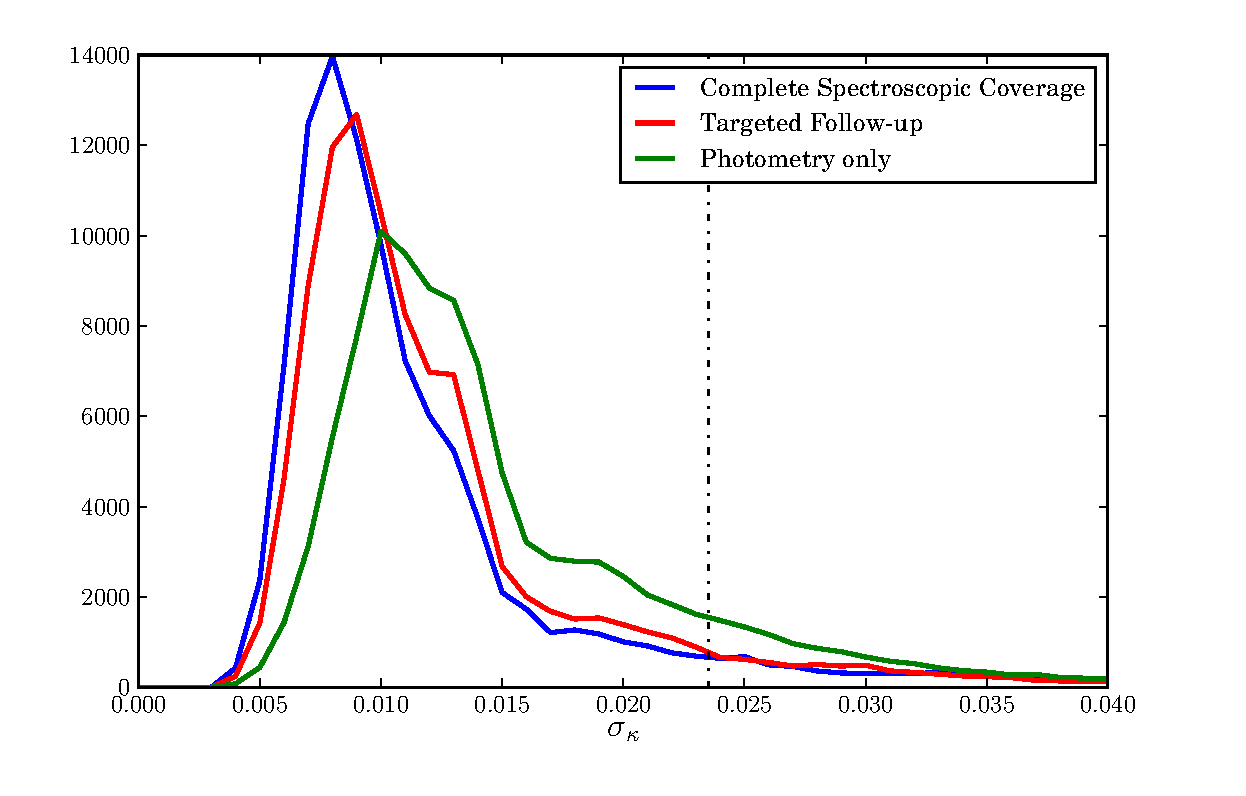
\includegraphics[width=\columnwidth]{figs/Width.eps}
\caption{The widths of the \infered PDFs $\pr(\kappax|\data)$ for
$10^5$ lines of sight, given different quality of data. 
Blue: spectroscopic redshift for every halo with $i<26$; 
Red: spectroscopic redshift for every halo with $i<23$, 
and every halo with $i<24$ within 1 arcminute, while all other objects just
have photometric redshifts;
Green: all the objects in the field have only photometric redshifts. The
vertical dot-dashed line marks the width of the global $\pr(\kappax)$ for all
lines of sight.}
\label{fig:reconwidths}
\end{figure}
%%%%%%%%%%%%%%%%%%%%%%%%%

%%%%%%%%%%%%%%%%%%%%%%%%%
\begin{figure}
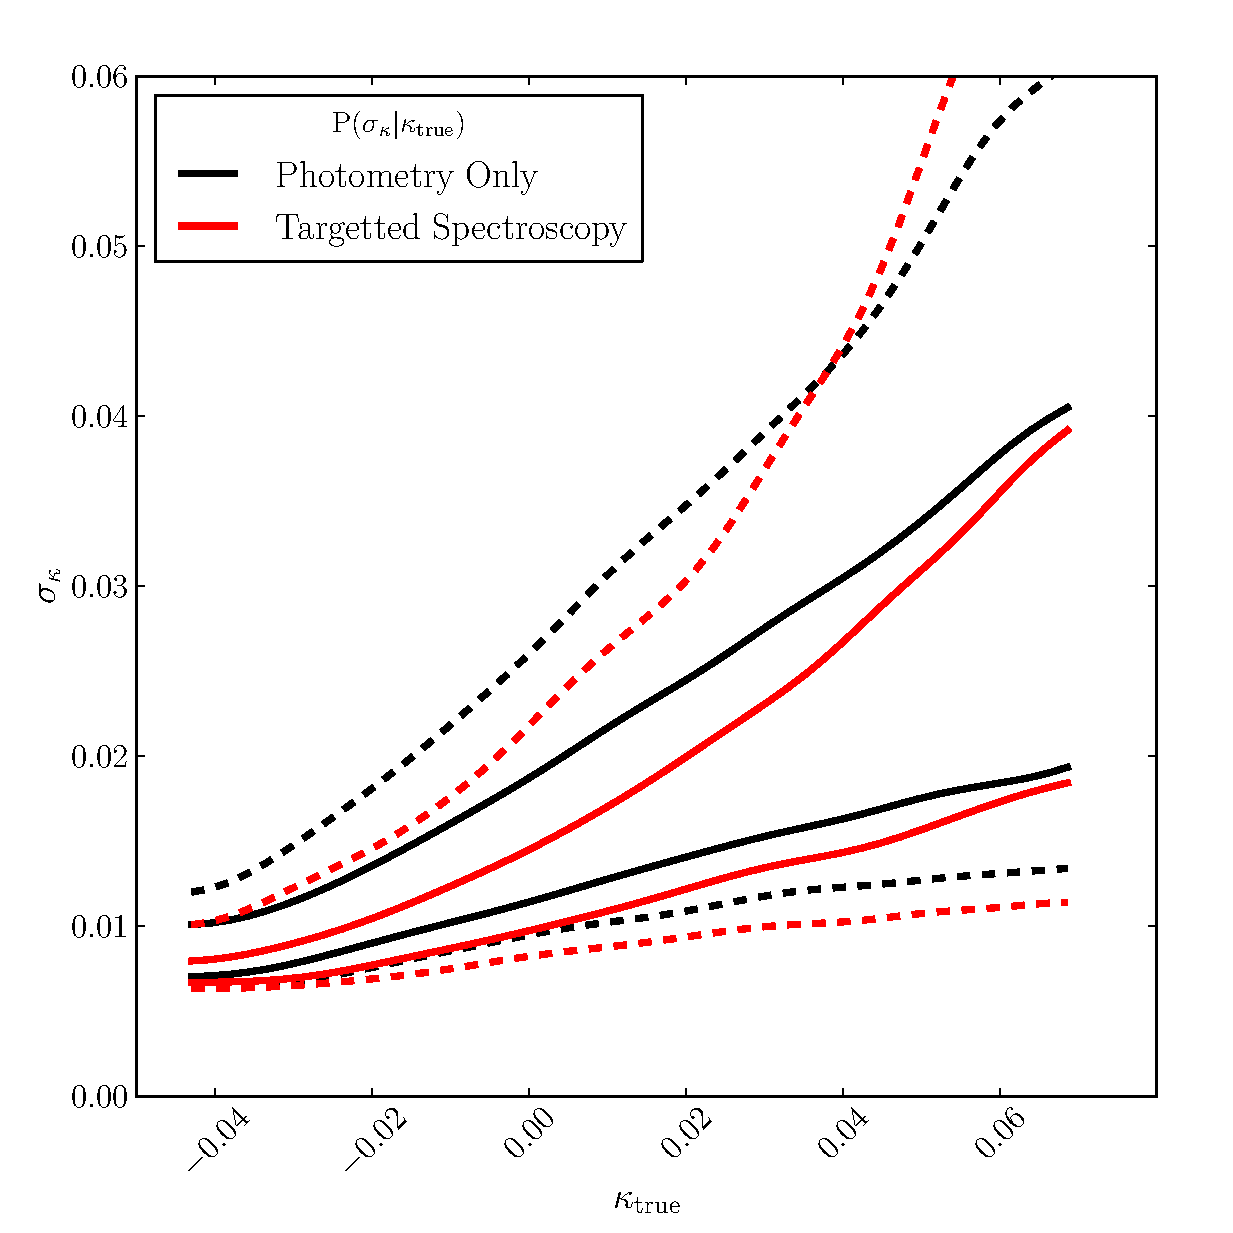
\includegraphics[width=\columnwidth]{figs/WidthvsHilbert.eps}
\caption{Width of the \infered PDF $\pr(\kappax|\data)$ as a function of 
the true convergence, $\kappaxtrue$, for two different data qualities. 
Black assumes only photometric redshifts for all objects,
while red assumes a campaign of targeted spectroscopy. The region between the
solid (dashed) lines contains 68\% (95\%) of lines-of-sight.}
\label{fig:widthsvsH}
\end{figure}
%%%%%%%%%%%%%%%%%%%%%%%%%

The best possible reconstructions of $\kappax$ will come from having a
spectroscopic redshift for every single object in each field.
\Fref{fig:reconwidths} shows the distribution of $\kappax$ posterior 
PDF widths for various data qualities: complete spectroscopic coverage results
in the smallest widths. In terms of telescope time, such a reconstruction
would likely be prohibitively expensive, but we investigate this scenario as
an ideal case. 

\comment{PJM: The following does not belong here because \Fref{fig:widthsvsH}
does not show results for spectroscopic redshifts only!}

Reconstructing the lines of sight with perfect knowledge of the
redshift but an uncertain stellar mass, we find that the width of
$\pr(\kappax|\data)$ grows with the expectation of $\kappax$ and the ray-traced $\kappatrue$
(\Fref{fig:widthsvsH}). The low $\kappax$ lines of sight are relatively empty,
and so there are few opportunities for uncertainties in the halo masses to
\propogate into $\kappax$ uncertainties; low $\kappax$ lines of sight can be reconstructed
more precisely than high $\kappax$ lines of sight.


% % % % % % % % % % % % % % % % % % % % % % % % % % % % % % % % % % % % % % % 

\subsection{Reconstructing $\kappax$ from photometry alone}

Inferring the stellar mass of a galaxy from its magnitude and colours requires
an estimate of how far away the galaxy is; without a spectroscopic redshift
the \infered stellar mass is less precise. However, obtaining photometry has
much lower observational cost; all upcoming large area photometric surveys
will reach 24th magnitude, providing sufficient data to reconstruct lines of
sight  {\it without} additional observations. In principle the photometric
redshift is correlated with the \infered stellar mass, however we do not model
this effect since the convergence from the outskirts of an individual halo is
only weakly \dependant on redshift at fixed mass due to the breadth of the
lensing kernel: the redshift uncertainty has only a small effect on the
inferred $\pr(\kappax|\data)$ in comparison to that of  the uncertain stellar
masses.  With only photometric redshifts, the uncertainty on $\kappah$ is
larger than in the spectroscopic case, and this \propogates into a broader
$\pr(\kappax|\data)$, as can be seen in \Fref{fig:reconwidths}. However, the
photometric reconstruction still typically produces a 50\% improvement
compared to the precision of the global $\pr(\kappax)$. 

\tom{With photometric data alone, $\kappah^{\rm med}$ can shift by $\sim$0.01
relative to $\kappah^{\rm med}$ given spectroscopic coverage. Since  the
$\kappax$ contribution of voids cannot change with data quality, the shift in
$\kappah^{\rm med}$ must be due to the asymmetric propagation of stellar mass
uncertainties into $\kappax$ uncertainties. As the stellar mass uncertainty
increases, $\kappah^{\rm med}$ is pushed higher.  To correctly calibrate 
$\pr(\kappax|\kappah^{\rm med},\data)$ one {\it must} include the data quality
used to generate $\kappah^{\rm med}$.}

We find that the width of $\pr(\kappax|\data)$ grows with the expectation
value of $\kappax$; this is shown in \Fref{fig:widthsvsH}. The low $\kappax$
lines of sight are relatively empty, and so there are few opportunities for
uncertainties in the halo masses to \propogate into $\kappax$ uncertainties.

%\flag{Is there a simple approximation for $\kappax$ and $\sigma_{\kappa}$ as a
%function of $\kappaxtrue$? This would be useful when making forecasts, writing
%proposals etc...}
%
%TEC: No. It's also not relevant to proposals since kappatrue isnt observable. One can ask is there
%a formula for sigmakappa given the expectation value of kappax. The answer to that is
%yes, but it depends on data quality. Concerning forecasting yes we would 
%want to use a simple approximation, but I don't think it has a place in this paper.
%When you/I/someone does the forecasting I'd like to be involved; I'll make the
%approximation then.


% % % % % % % % % % % % % % % % % % % % % % % % % % % % % % % % % % % % % % % 

\subsection{Reconstructing $\kappax$ with partial spectroscopic coverage}
\label{sec:obsMstar+z:targetedspec}

While a fully photometric reconstruction provides useful constraints on
$\pr(\kappax|\data)$, targeted spectroscopy can provide additional constraints
on the masses and redshifts of halos whose $\kappah$ contributions have the
largest absolute uncertainty. Obtaining spectra of bright ($i<22$) objects is
relatively fast with large telescopes: however, we find that if spectroscopic
redshifts were known for all $i<22$ galaxies in our fields the reconstruction
improves only slightly over the purely photometric reconstruction,  although
the improvement can depend strongly on the details of the particular line of
sight. Obtaining spectra for fainter objects would be correspondingly more
expensive, but if spectroscopic redshifts could be obtained for all $i<23$
galaxies (as part of a futuristic baryon acoustic oscillation survey, for
example) and all $i<24$ galaxies within 1 arcminute of the line of sight, then
we find that the $\pr(\kappax|\data)$ would be almost as precise as that from
having complete spectroscopic coverage (\Fref{fig:reconwidths}). If any object is
extremely close to the lines of sight our approximation of weakly lensing
mass-sheets will break down; also, neglecting baryonic effects will also be a poor
approximation; a spectrum will be needed
to adequately model systems with very well alligned pertrubers.
Consistent with our previous findings, the lowest $\kappax$ lines of
sight have the most constrained $\kappax$ PDFs.


%%%%%%%%%%%%%%%%%%%%%%%%%%%%%%%%%%%%%%%%%%%%%%%%%%%%%%%%%%%%%%%%%%%%%%%%%%%%%%

\section{Systematic Errors due to Sample Selection}
\label{sec:biases}


\begin{figure*}
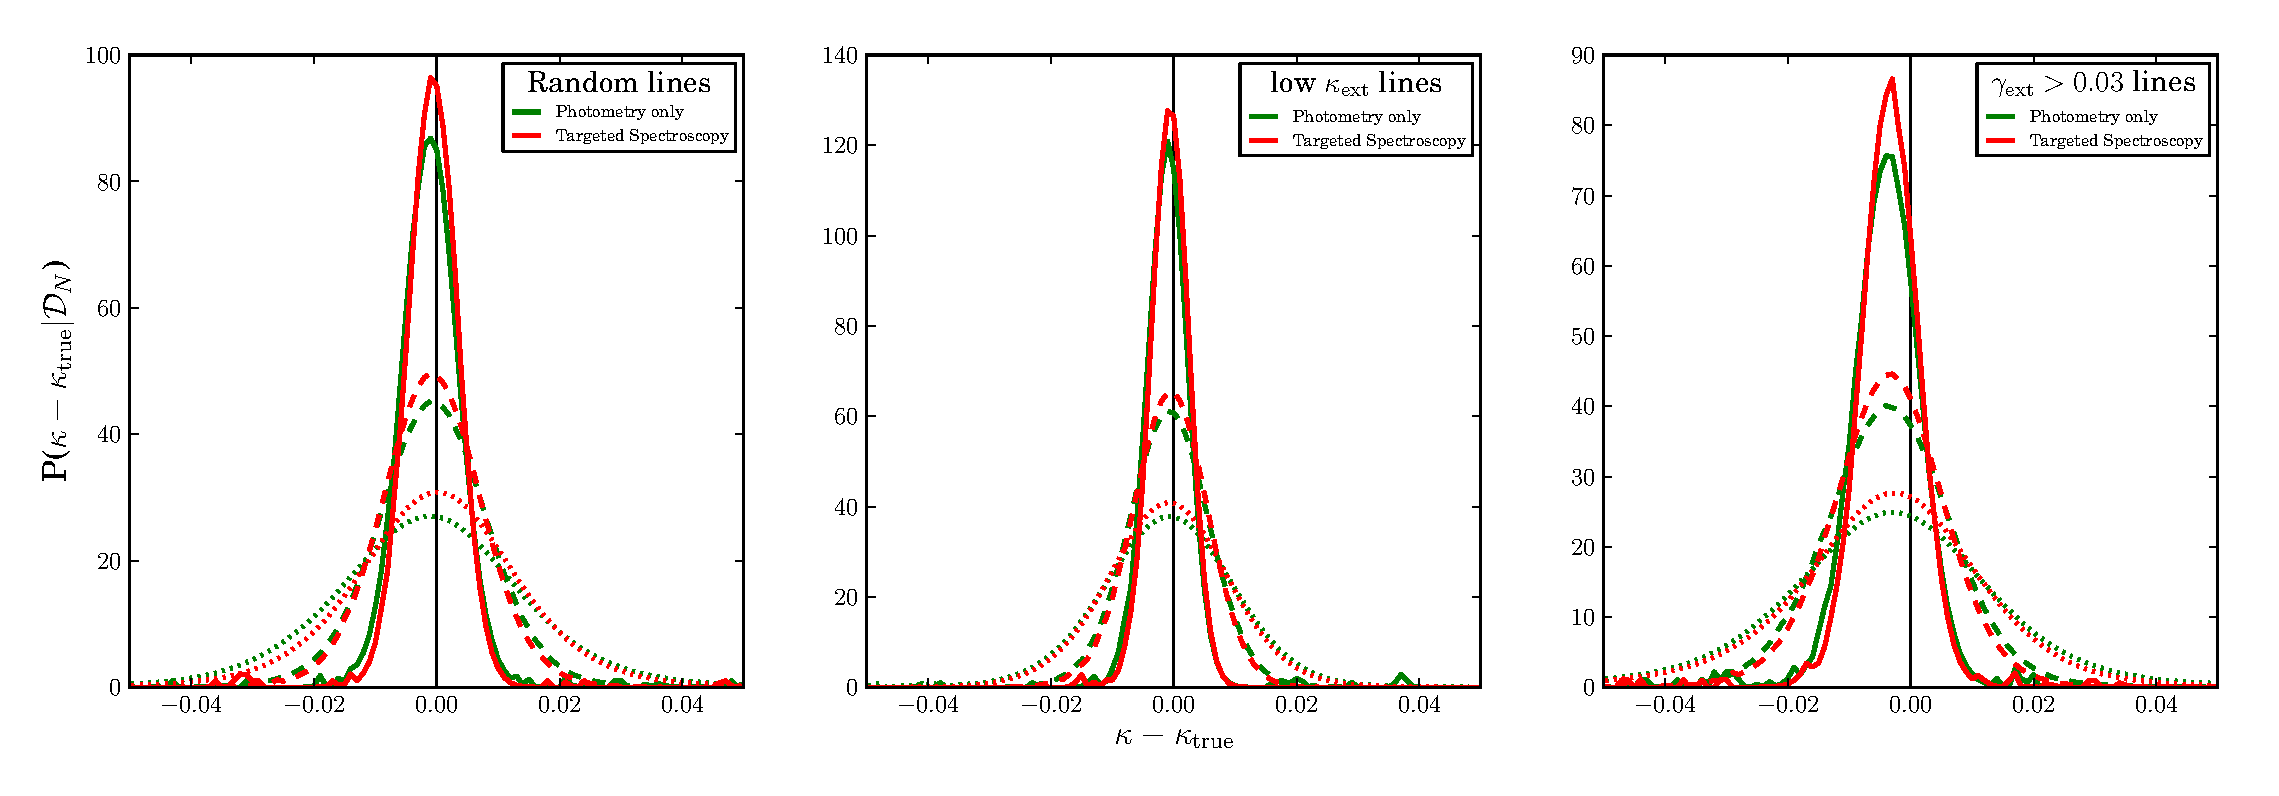
\includegraphics[width=\textwidth]{figs/biasplots.eps}
\caption{Accuracy in $\kappax$ from combining samples of lenses.  These plots
show the expectation value of $\prod_{i=1}^N \pr_i(\kappax-\kappaxtrue|\data)$ --
deviations from zero represent biases. The solid, dashed and dotted lines
correspond to combinations of  20, 5 and 2 sightlines respectively. Black
lines show the results \infered from photometry alone, whilst red lines show
the results  from the same targeted spectroscopy campaign described in 
\Sref{sec:obsMstar+z:targetedspec}. The three panels correspond to samples of
sightlines selected in different ways. Left: randomly selected lines of
sight.  Centre: sightlines randomly selected from the 33\% of lines whose
P($\kappax$) is most tightly constrained by our model.  Right: lines of sight
with external shear of 0.05 or greater.}
\label{fig:biasplots}
\end{figure*}

While it is good to reconstruct $\kappax$ precisely, it is more important that
$\kappax$ is reconstructed accurately. The reconstruction must not be biased. 
We quantify the accuracy of our reconstructed $\pr(\kappax|\data)$ in the
following way. By shifting the \infered $\pr(\kappax|\data)$ for each line of
sight by the true (ray-traced) convergence, we obtain a  PDF that should be
centred on zero; these offset PDFs can be multiplied together for multiple
lines of sight to emulate a joint likelihood analysis, and then test for
possible bias in it:
\be
\label{eq:bias}
\mathcal{P}_N = \prod_{i=1}^N \pr_i(\kappax-\kappax^{\rm true}|\data)
\ee
In this section, we quantify the bias as the size of the deviation in the
expectation value of $\mathcal{P}_N$ from zero. If the bias of $\mathcal{P}_N$
is smaller than the half-width of $\mathcal{P}_N$, our $\kappax$ inferences
can be considered accurate. Since the width of $\mathcal{P}_N$ decreases as
more sightlines are combined, a small bias will always 
eventually be found. In the context of measuring time-delay distance at the 
one percent level, the expectation value of $|\mathcal{P}_N|$ needs to be 
significantly less than 0.01. \tom{External convergence is not the only source
of uncertainty in measuring time-delay distance. Since the statistical
distance uncertainties due to lens modelling and time delay estimation are
likely to be at the 3-4\% level \citep{SuyuEtal2010}, convolving
$\mathcal{P}_N$ with a Gaussian of width $0.04/\sqrt{N}$ is a reasonable
approximation for the likely final uncertainty on time-delay distance.}


% \comment{From Sherry:
% Re: $P_N$:
% Not sure that this is the best way to quantify bias.  First of all, this
% doesn't include the modeling error of $\sim3-4\%$, so the number of lenses listed
% (for when <$P_N$> = half width of $P_N$) is underestimated.  Also, with this
% definition, a large number of lenses could be described as "biased" even if
% the resulting shift is say 0.0001, which won't really trouble us at all.  For
% example, what would the distributions look like in Fig.8 with 100 lenses? 
% Since the peaks of the red curves are within 0.01 of kappa_true, I would
% suspect that with a large number of lenses, the corresponding red curve would
% be within 0.01 of kappa_true.  The present day goal is to get H0 to 1\%, and
% it would be good to state somewhere that with targeted spectroscopy, one could
% recover kext at the 1\% level with a large sample of lenses.}

The source of systematic error that we investigate in this paper  is that of
sample selection: we define three different example selections of lines of
sight, and compute the bias  \phil{that would result (if left unaccounted
for)} in each one in turn, as a function of data quality. The results
described below are illustrated in \Fref{fig:biasplots}.


% % % % % % % % % % % % % % % % % % % % % % % % % % % % % % % % % % % % % % % 

\subsection{Selecting random lines of sight}
\label{sec:bias:random}

We first consider a purely random selection of lines of sight. With the purely
photometric reconstruction, there is no evidence of bias, even after combining
20 lines of sight. \tom{This result is a sanity check: if we had chosen lines
of sight with identical $\kappah^{\rm med}$ rather than $\kappah^{\rm
med}\pm0.003$, randomly selected lines of sight would have zero bias by
construction}. If lines of sight hosting time delay lenses are truely random, 
our method allows $\kappax$ to be reconstructed without inducing a bias (under
the basic assumptions that the universe is like the calibration simulation,
and the correct stellar-mass to halo-mass relation has been used). 


% % % % % % % % % % % % % % % % % % % % % % % % % % % % % % % % % % % % % % % 

\subsection{Selecting only the lines of sight with narrow $\pr(\kappax|\data)$}
\label{sec:bias:tightPDF}

Since follow-up campaigns (such as high resolution imaging, or time
variability monitoring) are expensive, it is likely that only a subset of
detected objects will be observed further. By pre-selecting objects that have 
the best-constrained convergence, the cosmological value per lens can be
increased. However, this selection \phil{(like any other)}
has the potential to induce a bias. It is
likely that only photometry will be available at the time of sub-sample
selection (although spectroscopic follow-up might be conducted at a later
date). We mimic such a selection by drawing lines of sight only from those in
the lowest third of $\sigma_{\kappa}$, given a purely photometric
reconstruction of their fields. 

We find that selecting the most tightly constrained lines of sight in this way
does not introduce a significant bias:  our reconstruction is most accurate
for the lowest $\kappax$ lines of sight. Combining 20 such systems, the bias
is at the 0.001 level.

Photometry of the field seems to be sufficient to adequately select these
empty lines of sight.  However, 
since lenses are typically massive galaxies and hence found in locally over-dense
environments, it is unlikely that  an almost empty line of sight would
actually  contain a lens; \phil{what we can say is that if the local
environment can be identified spectroscopically, and then the line
of sight mass distribution reconstructed using our method, selecting lenses
with low, well-constrained values of $\kappax$ will lead to an increase in
distance precision at no cost in bias.}

% % % % % % % % % % % % % % % % % % % % % % % % % % % % % % % % % % % % % % % 

\subsection{Selecting only high shear lines of sight}
\label{sec:bias:tightPDF}

Time delay lenses are often selected for follow-up based on their images'
brightness (to make monitoring observations less expensive), their images'
separation (to decrease the covariance between the ground-based image
light-curves), or the fact that they are quadruply-imaging rather than
doubly-imaging (since this yields 3 time delays instead of 1, a higher
magnification and a more informative Einstein Ring system). All three of these
properties favour lenses with high convergence and shear along their lines of
sight. Focusing on the quad selection, we might expect many of these systems
to have significant external shear (since the cross-section for 4 image
production is so sensitive to ellipticity in the lens mass distribution (or
equivalently, external shear due to the lens' environment). 

\phil{We can test the impact of such a shear selection by selecting only lines
of sight with an external shear above some threshold.  We define a somewhat
extreme selection  of $\gammax>0.05$, and find that in this sample, $\kappax$
would be systematically underestimated at the $\sim$0.008 level (corresponding
to a 0.8\% systematic error in distance).}  In the absence of other sources of
uncertainty, this systematic error would be significant in a sample of just 5
lenses; when including other time-delay distance uncertainties a 0.8\% bias would be
significant for $\sim$20 lenses. This systematic error is mitigated if only the lines of sight with both
$\gammax>0.05$ and well constrained $\pr(\kappax|\data)$ are used, but in this
case a bias at the $\sim$0.005 level remains. 

While $\gammax>0.05$ is likely to be a much stronger selection than would
occur in reality, it is  nevertheless worth noting from this example that the
reconstruction \proceedure \phil{can be biased if lens selection functions are
extreme and unaccounted for.} Since our model does not include shear
constraints it is not surprising that a selection function based on shear can
induce a bias. A more sophisticated model that includes the shear recovered
from the lens modelling might be less susceptible to this bias.

The halo model can also be used to estimate the external shear along a line of
sight: shear is an observable that can be extracted from strong lens
modelling. However, there is a degeneracy between internal and external shear.
When the Einstein Ring imaging data are very good it is possible to
disentangle external and internal shear \citep[\eg][]{SuyuEtal2010}, but there
are still significant uncertainties. \citet{WongEtal2011} attempted to match
the shear from strong lens models with a reconstruction of the local lens
group environment, but found a tension between the strong lens model and the
reconstruction of the environment. Given the \citet{WongEtal2011} results, it
is unclear whether the external shear from lens models can be reconciled with
a line-of-sight reconstruction. Alternatively, it may be possible  to infer
external shear using weak lensing information from near the line of sight.  If
the true external shear can be measured, it provides an additional constraint
on which of the \MS lines of sight are similar to the reconstructed line of
sight. \citet{SuyuEtal2012} found that in the case of 
RXJ1131-1231, combining shear constraints
with galaxy number count over-density gave a significantly different
$\pr(\kappax|\gamma,N_{45})$ compared to the PDF from number count
over-density alone, $\pr(\kappax|N_{45})$.

Extending our model to include shear we find that given
perfect knowledge of the halo mass and redshift the ray-traced external shear
$\gamma$ and the reconstructed external shear $\gamma_{\mathrm{h}}$  are
similar, with 68 percent of lines obeying
\be
\label{eq:shearineq}
|{\pmb{\gamma}_{\mathrm{ext}}-\pmb{\gamma}_{\mathrm{h}}}| < \mathrm{0.025}
\ee 
Future work should investigate whether $\gamma_{\mathrm{h}}$ can be used
to improve the accuracy and precision of $\kappax$ estimation, given a
reconstruction of the line of sight. 

%%%%%%%%%%%%%%%%%%%%%%%%%%%%%%%%%%%%%%%%%%%%%%%%%%%%%%%%%%%%%%%%%%%%%%%%%%%%%%

\section{Systematic Errors due to using an incorrect Stellar Mass--Halo Mass Relation}
\label{sec:SHAMfail}

\begin{figure*}
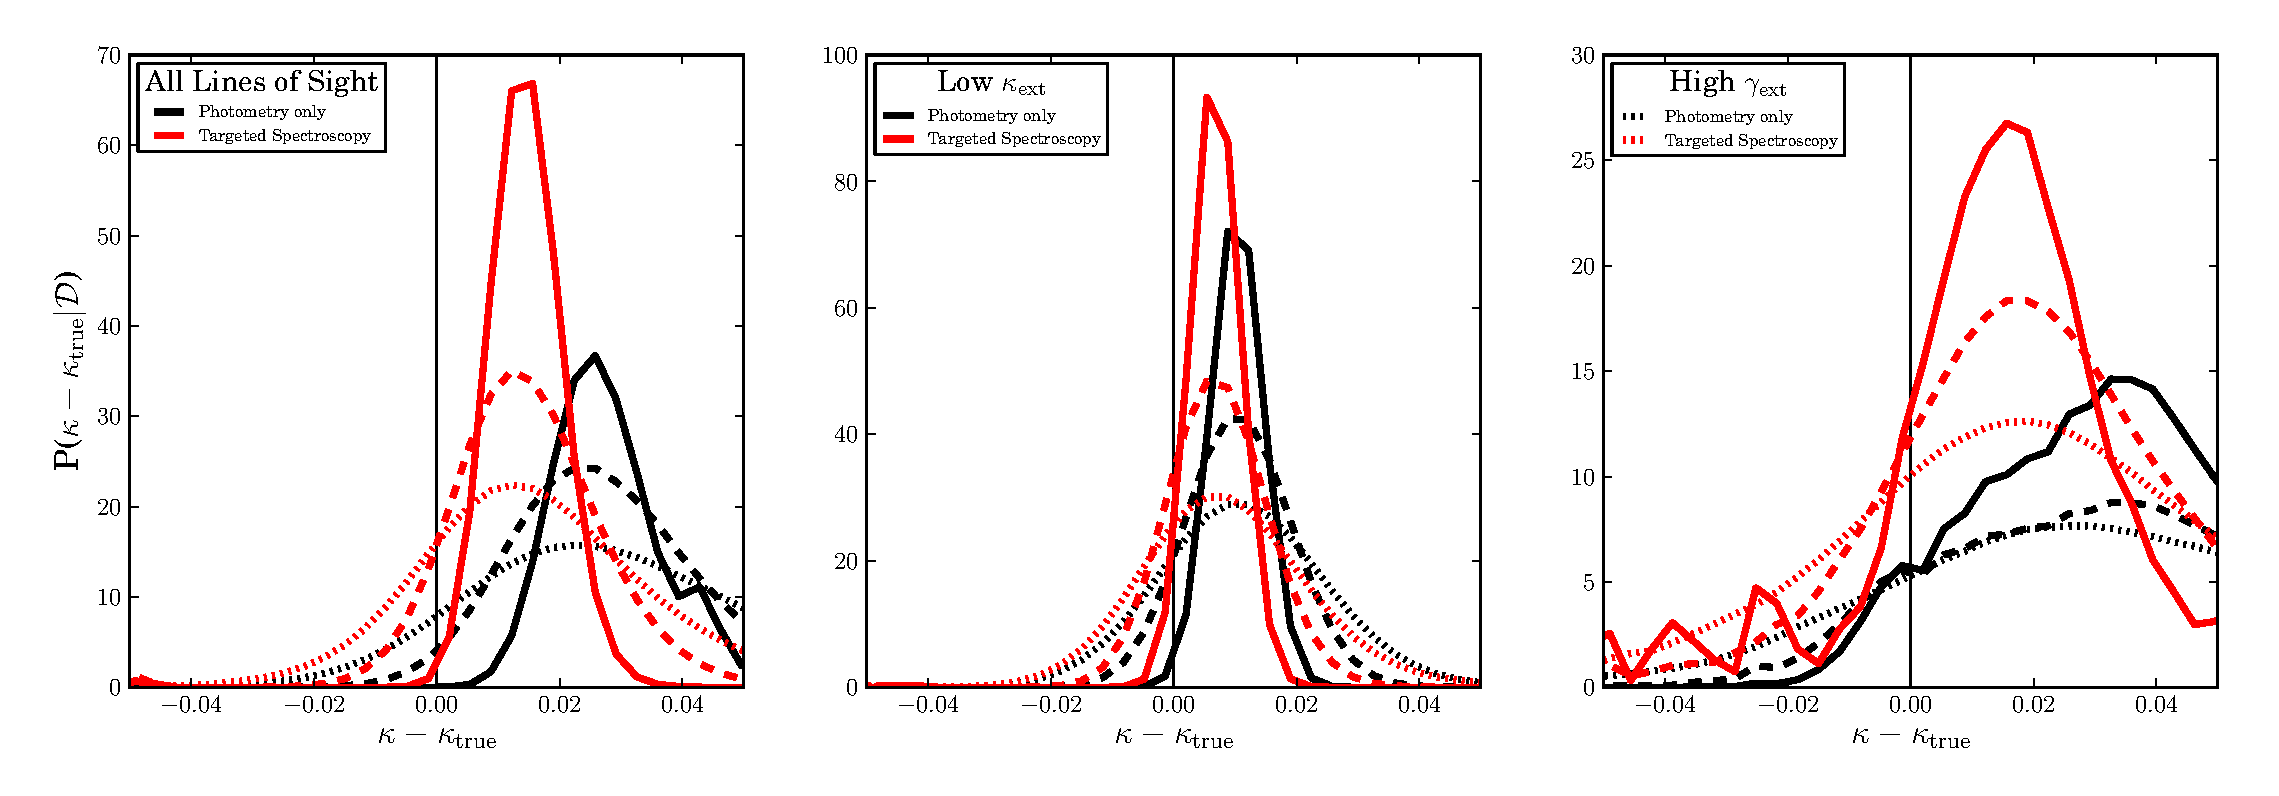
\includegraphics[width=\textwidth]{figs/SHAMbias.eps}
\caption{Systematic bias in $\kappax$ due to reconstructing lines of sight with the wrong stellar mass--halo mass relation. The real stellar masses were created using the relation of \citet{MosterEtal2010}, but the reconstruction and calibration assumes the relation of \citet{BehrooziEtal2010}.  These plots
show the expectation value of $\prod_{i=1}^N \pr_i(\kappax-\kappaxtrue|\data)$ --
deviations from zero represent biases. The solid, dashed and dotted lines
correspond to combinations of  20, 5 and 2 sightlines respectively. Black
lines show the results \infered from photometry alone, whilst red lines show
the results  from the same targeted spectroscopy campaign described in 
\Sref{sec:obsMstar+z:targetedspec}. The three panels correspond to samples of
sightlines selected in different ways. Left: randomly selected lines of
sight.  Centre: sightlines randomly selected from the 33\% of lines whose
P($\kappax$) is most tightly constrained by our model.  Right: lines of sight
with external shear of 0.05 or greater.}
\label{fig:SHAMbias}
\end{figure*}

\new{
Throughout this work we have assumed that the universe's halos are populated with galaxies whose stellar masses are determined purely by the \citet{BehrooziEtal2010} Stellar Mass--Halo Mass relation. The real universe is unlikely to follow this relation perfectly; the result is that an ensemble of real lines of sight will differ from the ensemble of calibration lines of sight, potentially introducing a systematic error to the reconstructed convergence.

It is hard to test the size of this sytematic error, since we do not know how much the real universe differs from the chosen Stellar Mass--Halo Mass relation. As wider and deeper surveys are conducted more data will become available with which to construct the Stellar Mass--Halo Mass relation; this should drive the infered Stellar Mass--Halo Mass relation closer to the truth. We are only interested in testing the effect of changing the Stellar Mass--Halo Mass relation in a way that is consistant with observational constraints; improving the observational contraints on the Stellar Mass--Halo Mass relation will decrease the the size of the systematic error on reconstructed $\kappax$ induced by assuming a specfic Stellar Mass--Halo Mass relation.

To estimate the potential size of this systematic error we use the Behroozi relation to generate the stellar masses of our calibration lines of sight, but the stellar mass--halo mass relation of Moster for the ``real'' lines of sight that are reconstructed. For halos masses of $\sim 10^{12} \Msun$ both stellar mass--halo mass relations estimate a stellar mass of $\sim 10^{10.5} \Msun$, but for halos more massive that this the stellar masses generated from the Moster relation are systematically higher than those generated from the Behroozi relation. At halo masses of $\sim 10^{14} \Msun$ the best fit stellar masses differ by $\sim 0.25$ dex. 

Applying our Behroozi--based reconstruction to lines of sight with Moster stellar masses results in systematically overestimating $\kappax$. In \Fref{fig:SHAMbias} we show the resulting bias on the inferred $\kappax$ after combining several lines of sight. With a purely photometric reconstruction there is a typical systematic bias of $\sim 0.025$ on the reconstructed convergence, although it can be shrunk to $\sim 0.01$ if only the low $\kappax$ lines of sight are used, however for the high shear lines of sight the bias is $\sim 0.04$. It is not suprising that the low $\kappax$ lines of sight are least affected by changes in the stellar mass--halo mass relation. Low $\kappax$ lines of sight are relatively empty hence their $\kappah$ values are small and do not change significantly with stellar mass--halo mass relation. The high shear lines of sight have significantly overestimated $\kappax$ since they tend to lie close to massive halos. This is the regime where the Moster and Behroozi relations are most different. Interestingly overestimating the $\kappah$ values of high shear lines of sight pushes them into the region where the $\kappah$ to $\kappax$ calibration is least certain; this has significantly decreased the precision of the reconstructed $\kappax$. 

Despite the systematic errors the photometric reconstruction is still sufficient to choose the best lines of sight for spectroscopic follow-up. With targetted spectroscopy the systematic error decreases to $\sim 0.014$ for the ensemble, $\sim 0.005$ for the low kappa sample and $\sim 0.018$ for the high shear sample. This result provides further motivation for prioritizing the lenses that reside on the underdense lines of sight.

The systematic errors reported herein may be overly pessimistic; the bias is due to differences in the stellar masses predicted for high mass halos. If observations can discriminate between the high mass end of the Behroozi and Moster relations then the systematic error on the reconstruction will decrease.
}

%%%%%%%%%%%%%%%%%%%%%%%%%%%%%%%%%%%%%%%%%%%%%%%%%%%%%%%%%%%%%%%%%%%%%%%%%
%\section{Improving precision by including additional information}
%\notes{placeholder for shear}
%%%%%%%%%%%%%%%%%%%%%%%%%%%%%%%%%%%%%%%%%%%%%%%%%%%%%%%%%%%%%%%%%%%%%%%%%

\section{Discussion}
\label{sec:discuss}

% \comments{
% We have shown that reconstructing the matter due to halos along any line of
% sight can improve the constraints on the external convergence along that line
% of sight, with, depending on sample selection,  the width of
% $\pr(\kappax|\data)$ being up to a factor of two smaller than the global
% $\pr(\kappax)$, and  we have quantified the residual bias in the $\kappax$
% estimates under our calibration assumptions. We now revisit these assumptions.
% }

The total convergence along a line of sight is strongly correlated with the
reconstructed $\kappah$. However, since our model ignores voids and assumes
all halos follow a spherical truncated-NFW profile our halo model does not
include all of the relevant physics; hence, the width of our resulting
$\pr(\kappax|\data)$ is still typically $\sim$0.01 for any given lightcone,
even assuming perfect knowledge of every halo's virial mass and redshift. To
make further progress a more advanced treatment of both voids and halos will
be needed. \citet{KarpenkaEtal2012} find that their supernova data prefer, in
the context of their simple halo model, a truncated isothermal profile for the
galaxy mass distributions. Galaxy-galaxy and cluster-galaxy  lensing studies
\citep[\eg][]{GavazziEtal2007,JohnstonEtal2007, LagattutaEtal2010} also suggest an approximately
isothermal profile for the mass-shear correlation function; however, at large
radii these profiles are dominated by the effects of neighbouring halos, which
are already taken into account by our model.  Further iterations on the
analysis presented here should include the stellar mass distributions that
cause the isothermal density profiles in the centres of galaxies, although we
do not expect this to have a big impact on the reconstructions. Likewise, 
halo ellipticity
may have some small effect on the predicted convergence. It
is possible that baryonic physics may alter the radial profile of dark
matter halos, even on large scales. \citet{Semboloni+2012} found that baryonic
physics had a 30-40\% impact on three-point shear statistics, it is unclear
how baryons affect one-point convergence statistics compared to the pure dark
matter simulations used in this work.

Clusters, filaments and voids are more difficult to model, but simple forms
could in principle be derived from the structures found in the simulations,
and included in the halo model in some way.  Most importantly for the highest
$\kappax$ lines of sight will be a better group and cluster model:
\citet{MomchevaEtal2006} and  \citet{WongEtal2011} recommend using models
where dark mass is assigned to both galaxy-scale halos and halos for the
groups and clusters they occupy. To make this work, one could incorporate a
group and cluster finder, and then infer halo mass from optical richness
\citep[\eg][]{MaxBCG} in tandem with BCG stellar mass. \new{A group finder would also
allow us to identify central and satellites galaxies; in this work we have neglected
the differences between central halos and satellites. However, given perfect knowledge of halo masses
we found that only in 5 percent of sightlines do satellites
contribute over 20 percent of the sightline's total $\kappax$. Introducing a group finder
is unlikely to provide major improvement to the reconstruction of satellites.}
\tom{Meanwhile,
improving the modelling of voids could be done using suggestions by
\citet{voids2} or \citet{voids1} combined with a void finder such as in
\citet{voids3}. Combining an advanced halo model with a void model will allow
a direct test of the halo approximation: using real photometric data one could
reconstruct lines of sight and compare against measured weak lensing shears.
This would ensure that the reconstruction model reproduces the contents of the
real universe, rather than a particular simulation.}

% \comments{Interestingly, we have found that it is the most empty lines of sight that 
% can be reconstructed with the highest precision. $\kappax$ estimates for empty
% lines of sight receive few contributions from halos, and a large contribution
% from voids; since they have the tightest PDFs after the reconstruction it
% seems that our model's biggest uncertainties are driven by naively
% reconstructing halos rather than neglecting voids. With a photometric
% reconstruction of the field there is a significant broadening, but the
% resulting precision is still typically 50\%  higher than using the global
% $\kappax$ distribution.
% 
% Since the uncertainty on $\pr(\kappax|\data)$ is $\sim$0.01 even
% with perfect knowledge of halo mass and redshift, it seems that modelling uncertainties
% from voids, deviations from sphericity and dark matter clumping within the
% main halo dominate the total $\kappax$ uncertainty even with very
% uncertain stellar masses. Inferring halo ellipticity and dark matter
% clumping will likely always remain a difficulty for line of sight
% reconstruction; but as \Fref{fig:magcut} shows, observing deeper
% than 24th magnitude does not significantly help the reconstruction.
% }

% \comments{For a small fraction of lines of sight, $\pr(\kappax|\data)$ remains very
% broad even after applying our reconstruction; these lines of sight are
% typically the most over-dense lines of sight in the universe. For
% time-delay cosmography the most observationally expensive tasks are the
% light-curve monitoring and high resolution follow-up imaging and spectroscopy,
% while making photometric observations of a
% 4$\times$4 arcminute patch of sky survey down to 24th magnitude is
% relatively cheap. We have shown that with a single epoch observation of
% the region around a strong lens it is possible to infer $\pr(\kappax|\data)$.
% If a line of sight has a broad $\pr(\kappax|\data)$ it can be rejected {\it
% before} the investment of follow-up. We find that
% selecting only the lines of sight with the most tightly constrained
% $\pr(\kappax)$ does not induce a bias in $\kappax$, and hence distance.
% For the most over-dense lines of sight,
% the precision of $\pr(\kappax|\data)$ is improved noticeably by the addition
% of spectroscopic information; currently insufficient time-delay systems are
% know to choose a subset based on their reconstructed $\pr(\kappax|\data)$.
% Spectroscopic coverage will definitely be useful for extracting cosmology from
% over-dense lines of sight.
% }
% %%%%%%%%%%%%%%%%%%%%%%%%%%%%%%
% \comments{%
% \begin{figure}
% 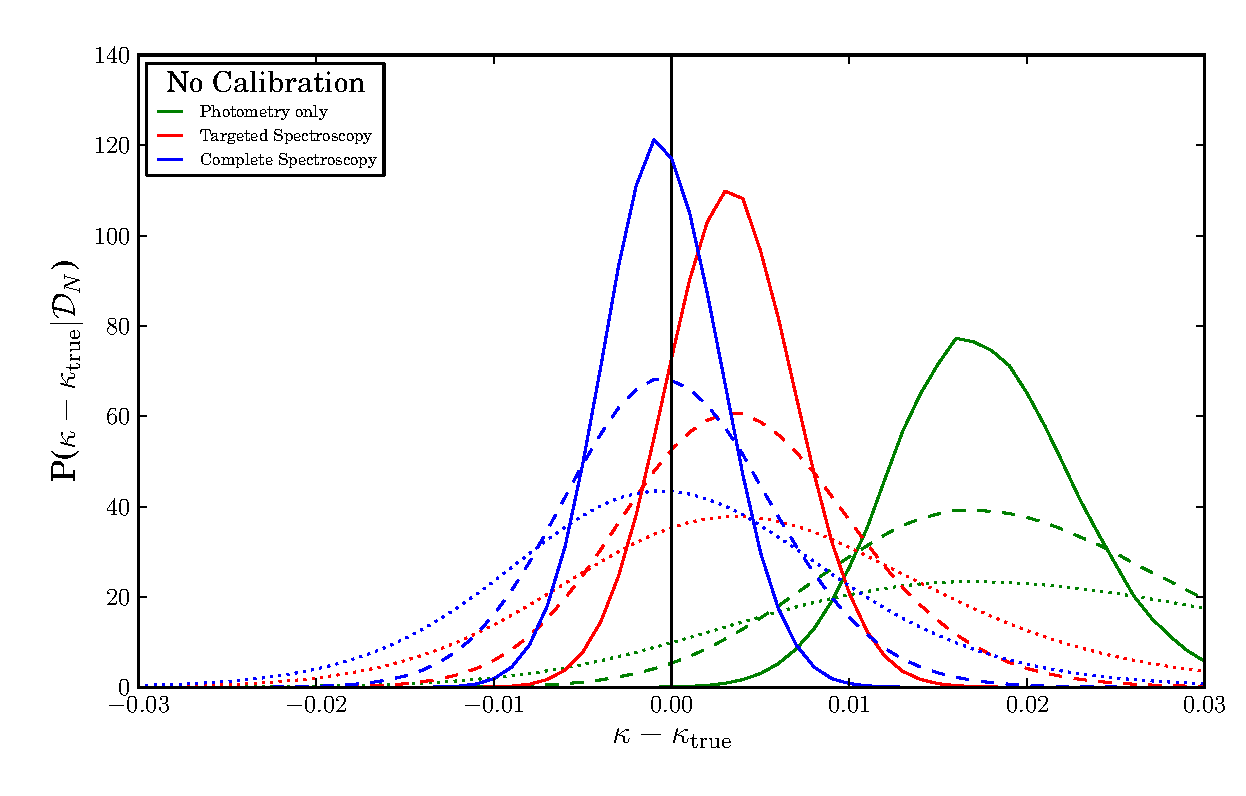
\includegraphics[width=\columnwidth]{figs/biasplots3.eps}
% \caption{Convergence estimation accuracy using the full  $\pr(\kappax|\kappah)$
% distribution, rather than its median.  As in \Fref{fig:biasplots}, solid,
% dashed and dotted lines show combinations of 20, 5 and 2 lines of sight
% respectively, while green lines show the inferences 
% from photometry alone, red lines from photometry and targeted spectroscopy 
% (assuming a spectroscopic redshift for all
% halos with $i<23$ and all halos within 1 arcminute and $i<24$), and blue lines
% from the unrealistic assumption of a spectroscopic redshift for all galaxies
% in the field. }
% \label{fig:no-median-tricks}
% \end{figure}
% }%
%%%%%%%%%%%%%%%%%%%%%%%%%%%%%%

The reduction of $\pr(\kappah|\data)$ to just its median value, before using
it to look up the appropriate $\pr(\kappax)$ from the simulated sightline
ensemble, is reminiscent of the procedure followed by \citet{SuyuEtal2010},
and Greene et al (submitted). The reconstruction method presented here can be
seen as the limiting case of the weightings explored by Greene et al: rather
than using weighted number counts in an aperture, we treat each galaxy
individually, and predict $\kappa_{\rm h,obs}^{\rm med}$ for use in their
place. Given photometry alone, our reconstruction represents a $\sim$50\% improvement of
the precision compared the number counts used in \citet{SuyuEtal2010}. Greene et al.
made important progress for the most over-dense lines of sight; our
reconstructions are $\sim$30\% more precise than those of Greene et al.
The use of relative overdensities by Suyu et al. and Greene et al. may decrease 
their sensitivity to the choice of calibration simulation; this work's use of
absolute convergence may be less robust to changes in the calibration simulation. 


% \comments{ One
% significant disadvantage of these types of method is that they impose a
% bottleneck in the flow of information. Once you have compressed to one number,
% it is difficult to incorporate more information later; you have to recompute
% all the calibrations. Using the full PDF for $\kappah$ is the more correct
% thing to do: at present, however, it suffers from significant bias in the
% photometric data case. \Fref{fig:no-median-tricks} shows how $\kappax$ is
% overestimated, as a result of the high scatter in halo mass for objects with 
% high stellar mass. As has already been noted, 
% future work should focus on increasing the precision of the halo
% mass estimates. 
% }

In this work, we have used  the \MS as a calibration tool. If the real
Universe is not like the \MS, then this calibration will be incorrect.
Repeating this study using a different simulation to make the test catalogues
would allow us to quantify the sensitivity of our results to the simulation
used. Similarly the use of a different semi-analytic model to paint galaxies
onto halos would enable similar exploration of these systematic errors. 
\citet{SuyuEtal2010}
used the relative over-density to mitigate the effect of simulatioan and
simulation, but it does not completely remove the dependence on simulation.
\new{We have tested the effect of using a different stellar mass--halo mass relation
and found that this can induce significant systematic biases if the true relation is unknown.} Future work should include
investigating the robustness of the reconstruction to these systematic errors \new{and develope proscriptions that mitigate against them}

% \comments{In particular, the method presented here is tied to the simulations at two
% points: the prior PDF for $\kappah$, and the conditional distribution
% $\pr(\kappax|\kappah)$ used to convert halo model convergence to total
% convergence. The first tie could potentially be avoided if the halo mass
% estimation gave rise to a reasonable $\pr(\kappah|\data)$ on its own.
% Possibilities for improving the precision of the halo mass estimation are
% discussed above. The second tie is more difficult, since breaking it means
% modelling the unseen mass structures and voids. It
% should be possible to infer hierarchically  the parameters of a flexible model
% for these things from the data itself, as demonstrated by
% \citet{KarpenkaEtal2012} (albeit under the assumption of scatter-free scaling
% relations) -- how this affects the cosmographic precision is to be
% investigated. When working with wide field imaging surveys,  weak lensing shears will be
% available around every line of sight:  fitting these with the halo models
% described here in order to constrain the hyper-parameters of the model presents a 
% possible test of our halo model prescription against real observations.
% }
%%%%%%%%%%%%%%%%%%%%%%%%%%%%%%%%%%%%%%%%%%%%%%%%%%%%%%%%%%%%%%%%%%%%%%%%%

\section{Conclusions}
\label{sec:conclude}

In this work we have investigated a simple halo model prescription for
reconstructing all the mass along a line of sight to an intermediate redshift
source. We have used the ray-traced lensing convergence along lines of sight
through the Millennium Simulation to calibrate estimates of the total
convergence made by summing the convergences due to each object in a
photometric catalogue. Having found that the reconstruction process is
accurate given this calibration and perfect knowledge of halo mass and
redshift, we investigated the effects of reasonable uncertainties in the
stellar mass and redshift of each halo, and propagated these uncertainties
into a $\pr(\kappax|\data)$ for each line of sight. We also defined three
different possible line of sight selections, and investigated the possible 
bias induced by these selections. We draw the following conclusions:

\begin{itemize} 

\item Despite our model's simplicity, its reconstructed $\kappah$ values are
good tracers of $\kappax$. $\kappah$ is biased due to our ignorance of voids,
groups and clusters, and the unseen mass in small halos and filaments, but we
find that this can be calibrated out using the Millenium Simulation
catalogues. We found that with perfect knowledge of every halo's mass and
redshift,  calibrated reconstruction of a typical line of sight  gives an
unbiased estimate of $\kappax$ that is not perfect, but is $1.8$ 
times more precise than the global
$\pr(\kappax)$. This factor quantifies the limit to which the halo model can
represent the external convergence due to line of sight mass structure.

\item With uncertain halo masses and redshifts, we find that
$\pr(\kappah|\data)$ can still be calibrated in order to infer
$\pr(\kappax|\data)$ from the ensemble of simulated lines of sight, but the
resulting PDFs tend to be much broader than for perfect halo mass and redshift
reconstructions.

\item It is very rare for halos further than 2 arcminutes from the line of
sight to make a significant contribution to $\pr(\kappax|\data)$; likewise, 
including
halos whose host galaxy is less luminous than $i=24$ does not significantly
improve our reconstructions.  A photometric survey to this depth of a
4$\times$4 arcminute patch around the target would approach the limiting
uncertainties of our simple reconstruction recipe, and yield a 
$\pr(\kappax|\data)$ that has, on average, a width of 0.016 (inducing a $\sim$1.6\%
uncertainty on time-delay distances). This is 1.5 times
less broad than the global $\pr(\kappax)$. 

\item  For the most over-dense lines of sight, the reconstruction produces a
broad PDF; conversely, we find that the lines of sight with the sharpest
inferred $\pr(\kappax|\data)$ are typically under-dense. Since the
reconstructions described here can be performed before follow-up time is
invested, it will be possible to select targets by the precision of their
$\kappax$ estimates. This will be useful in an era when there are more known
lenses than can be followed-up. Photometric data are sufficient to select the best lines of sight for
follow-up. Spectroscopic coverage helps to tighten  $\pr(\kappax|\data)$ for
most lines of sight.
% , but is of less use for low $\kappax$ lines of
% sight.

\item Selecting from the highest precision 33\% of the reconstructed lines of
sight results in a sample with low bias, $\sim$0.1\% in terms of the
time-delay distance. \tom{For these lines of sight the reconstructed
$\pr(\kappax|\data)$ induces a statistical uncertainty of $\sim$1\% on
individual time-delay distances.}

\item Conversely, selecting lines of sight with high shear ($|\gamma| > 0.05$; 
a somewhat extreme selection, but one that  could potentially arise from 
focusing on four-image or wide separation lenses) results in a sample with
bias of 0.8\% in time delay distance (and hence $H_0$). Including realistic estimates of other
sources of uncertainty a systematic error of 0.8\% would become significant in
a sample of $\sim$20 lenses. The addition of shear constraints to our model might
alleviate this potential systematic.

\item \new{Reconstructing a line of sight with an incorrect stellar mass--halo mass relation can introduce systematic errors on the inferrred time-delay distance at the percent level. This error can only be reduced by tightening the observational limits on the stellar mass--halo mass relation at the high mass end.}

% \item With only a photometric reconstruction of all time delay lens fields,
% and following up only the systems with the most precise $\kappax$ estimates,
% the width of the dominant statistical uncertainty in time-delay cosmography
% can be halved, without inducing biases at the one percent level.

\end{itemize}

% PJM: Im not sure this is the right note to end on. 

% TEC: I liked it! but it's open to discussion.


% External convergence is not the only uncertainty in time delay cosmology, but
% for systems like B1608$+$656 it is the dominant one. For most lines of sight
% lens modelling induces uncertainties at the $\sim$4 percent
% level, which far exceeds the typical $\kappax$ uncertainties after applying our
% reconstruction \proceedure. By using reconstruction methods such as that
% explored here to select the most appropriate 
% lenses for follow-up, the uncertainties due to line of sight
% convergence will become a sub-dominant source of error.

While we have tested our reconstruction method against realistic simulations
of line of sight mass distributions in the Universe, our method is also 
calibrated to these simulations. Testing this assumption in the short term,
and replacing it with an empirical calibration (or hierarchical inference) in
the longer term, are worthy goals for future work. The halo model framework is
flexible enough to enable many such improvements, including, quite naturally,
the incorporation of more information from observations. 


%%%%%%%%%%%%%%%%%%%%%%%%%%%%%%%%%%%%%%%%%%%%%%%%%%%%%%%%%%%%%%%%%%%%%%%%
%%  ACKNOWLEDGMENTS
%%%%%%%%%%%%%%%%%%%%%%%%%%%%%%%%%%%%%%%%%%%%%%%%%%%%%%%%%%%%%%%%%%%%%%%%

\section*{Acknowledgements}
 
TEC thanks Vasily Belokurov for supervision, guidance and suggestions.
We thank Risa Wechsler and Peter Behroozi 
for useful discussions and suggestions. We are grateful to the referee
for suggesting improvements to the original manuscript.
TEC acknowledges support from STFC in the form of a research studentship.
%
PJM was given support by the Kavli Foundation and the Royal 
Society, in the form of research fellowships.
%
MWA \ldots
%
SH \ldots
%
SHS \ldots
%
TT acknowledges support from the NSF through CAREER award NSF-0642621,
and from the Packard Foundation through a Packard Research Fellowship.
% 
LVEK acknowledges the support by an NWO-VIDI programme subsidy
(programme number 639.042.505).
%
This research is supported in part by the National Science Foundation under
Grant No. PHY99-07949.



%%%%%%%%%%%%%%%%%%%%%%%%%%%%%%%%%%%%%%%%%%%%%%%%%%%%%%%%%%%%%%%%%%%%%%%%%%%%%%
%  APPENDICES
%%%%%%%%%%%%%%%%%%%%%%%%%%%%%%%%%%%%%%%%%%%%%%%%%%%%%%%%%%%%%%%%%%%%%%%%%%%%%%

\appendix

%%%%%%%%%%%%%%%%%%%%%%%%%%%%%%%%%%%%%%%%%%%%%%%%%%%%%%%%%%%%%%%%%%%%%%%%%%%%%%

\section{Inferring $\Mhalo$ given a noisy measurement of $\Mstarobs$}
\label{appendix:MSMH}

To estimate the convergence caused by a halo we need to know its mass; how can 
halo mass be \infered from a noisy estimate of the stellar mass $\Mstarobs$
of a galaxy at redshift $z$. We seek the posterior
PDF $\Pr(\Mhalo|\Mstarobs,z)$, which can be expanded as follows:

\begin{eqnarray}
&& \Pr(\Mhalo|\Mstarobs,z) = \notag\\
&& \int d\Mstar \Pr(\Mhalo|\Mstar,z) \Pr(\Mstar|\Mstarobs,z), \notag\\
&\propto& \int d\Mstar \Pr(\Mstarobs|\Mstar) \Pr(\Mstar|\Mhalo,z) \Pr(\Mhalo|z),
\label{eq:mhalo-mstar}
\end{eqnarray}
where we have used Bayes' Theorem twice to replace
$\Pr(\Mhalo|\Mstar,z) \Pr(\Mstar|z)$ with 
$\Pr(\Mstar|\Mhalo,z) \Pr(\Mhalo|z)$, and 
to invert $\Pr(\Mstar|\Mstarobs)$ into the sampling
distribution $\Pr(\Mstar|\Mstarobs)$, which we recognise as the likelihood
function for the observed stellar mass. Note that the ``true'' $\Mstar$ of the
galaxy is marginalised out: we are only interested in inferring the halo
mass. The last two terms in
\eqref{eq:mhalo-mstar} are the $\Mstar-\Mhalo$ relation from
\citet{BehrooziEtal2010}, and the halo mass function $\Pr(\Mhalo|z)$, at the
given redshift. We can
tabulate the product of these two from our Millennium Simulation catalogue,
constructing a two-dimensional histogram of halo masses and their associated
true stellar masses (drawn from the Behroozi relation). 

For each galaxy, we compute the likelihood function for its $\Mstarobs$ as a
function of the unknown $\Mstar$, and multiply it by our tabulated joint PDF.
This heavily downweights halos with $\Mstar$ values outside the observed
range. We then do the marginalisation integral by Monte Carlo, drawing
(two-dimensional) sample parameter vectors
from the down weighted histogram, discarding the $\Mstar$ values, and
constructing a one-dimensional histogram that is an estimate of
$\Pr(\Mhalo|\Mstarobs)$.

If the redshift of the galaxy is uncertain, we need to take this
uncertainty into account; for example, for each sample drawn from the
photometric redshift posterior PDF $\Pr(z|{\rm colors})$, we can draw a
sample $\Mhalo$ using the above procedure.

%%%%%%%%%%%%%%%%%%%%%%%%%%%%%%%%%%%%%%%%%%%%%%%%%%%%%%%%%%%%%%%%%%%%%%%%%%%%%%
%  REFERENCES
%%%%%%%%%%%%%%%%%%%%%%%%%%%%%%%%%%%%%%%%%%%%%%%%%%%%%%%%%%%%%%%%%%%%%%%%%%%%%%

% MNRAS does not use bibtex, input .bbl file instead. 
% Generate this in the makefile using bubble script in scriptutils:

% bubble -f paper-lcr.tex references.bib 
% %%%%%%%%%%%%%%%%%%%%%%%%%%%%%%%%%%%%%%%%%%%%%%%%%%%%%%%%%%%%%%%%%%%%%%%%
%
% Pangloss: Testing the reconstruction method
%
%%%%%%%%%%%%%%%%%%%%%%%%%%%%%%%%%%%%%%%%%%%%%%%%%%%%%%%%%%%%%%%%%%%%%%%%

\documentclass[useAMS,usenatbib,a4paper]{mn2e}
%% letterpaper
%% a4paper

%\voffset=-0.6in

% Packages:
\input psfig.sty
\usepackage{xspace}
\usepackage{graphicx}
\usepackage{amssymb}
\usepackage{amsmath}

% Macros:
% JOURNALS
\newcommand{\apj}{ApJ}
\newcommand{\apjl}{ApJL}
\newcommand{\apjs}{ApJS}
\newcommand{\mnras}{MNRAS}
\newcommand{\apss}{Ap \& SS}
\newcommand{\aap}{A\&A}
\newcommand{\aj}{AJ}
\newcommand{\prd}{Phys. Rev. D}
\newcommand{\nat}{Nature}
\newcommand{\araa}{ARA\&A}
\newcommand{\jgr}{J. Geophys. Res.}
\newcommand{\pasp}{PASP}

% MISC
\newcommand{\etal}{et~al.~}
\def\spose#1{\hbox  to 0pt{#1\hss}}  
\newcommand{\lta}{\mathrel{\spose{\lower 3pt\hbox{$\sim$}}\raise  2.0pt\hbox{$<$}}}
\newcommand{\gta}{\mathrel{\spose{\lower  3pt\hbox{$\sim$}}\raise 2.0pt\hbox{$>$}}}
\newcommand{\eg}{{\it e.g.\ }}
\newcommand{\ie}{{\it i.e.\ }}
\newcommand{\be}{\begin{equation}}
\newcommand{\ee}{\end{equation}}
\newcommand{\dee}{\, \mathrm{d} \!}
\newcommand{\bea}{\begin{eqnarray}}
\newcommand{\eea}{\end{eqnarray}}


% CROSS-REFERENCING
\def\Sref#1{Section~\ref{#1}\xspace}
\def\Fref#1{Figure~\ref{#1}\xspace}
\def\Tref#1{Table~\ref{#1}\xspace}
\def\Eref#1{Equation~\ref{#1}\xspace}
\def\Eqref#1{Eq.~(\ref{#1})\xspace}
\def\Aref#1{Appendix~\ref{#1}\xspace}

% UNITS
\newcommand{\kms}{\ifmmode  \,\rm km\,s^{-1} \else $\,\rm km\,s^{-1}  $ \fi }
\newcommand{\kpc}{\ifmmode  {\rm kpc}  \else ${\rm  kpc}$ \fi  }  
\newcommand{\pc}{\ifmmode  {\rm pc}  \else ${\rm pc}$ \fi  }  
\newcommand{\Msun}{\ifmmode {\rm M_{\odot}} \else ${\rm M_{\odot}}$ \fi} 
\newcommand{\Zsun}{\ifmmode {\rm Z_{\odot}} \else ${\rm Z_{\odot}}$ \fi} 
\newcommand{\yr}{\ifmmode yr^{-1} \else $yr^{-1}$ \fi} 
\newcommand{\hMsun}{\ifmmode h^{-1}\,\rm M_{\odot} \else $h^{-1}\,\rm M_{\odot}$ \fi}

% COSMOLOGY
\newcommand{\LCDM}{$\Lambda{\rm CDM}$}
\newcommand{\MS}{Millennium Simulation\xspace}

% LENSING
\def\zd{z_{\rm d}}
\def\zs{z_{\rm s}}
\def\Dd{D_{\rm d}}
\def\Ds{D_{\rm s}}

\def\Dt{D_{\Delta t}}

\def\Dds{D_{\rm ds}}
\def\Sigmacrit{\Sigma_{\rm crit}}
\def\REin{R_{\rm Ein}}
\def\MEin{M_{\rm Ein}}
\def\xkappa{\kappa_{\rm ext}}
\def\kappax{\kappa_{\rm ext}}
\def\kappaxtrue{\kappax^{\rm true}}
\def\kappah{\kappa_{\rm h}}
\def\kappav{\kappa_{\rm void}}
\def\kapparay{\kappa_{\rm raytrace}}
\def\kapparec{\kappa_{\rm reconstruction}}
\def\kappatrue{\kappa_{\rm true}}
\def\kappahalo{\kappa_{\rm halo}}
\def\Pkh{{\rm P}(\kappa_{\rm h})}
\def\Pk{{\rm P}(\kappa)}
\def\kappah{\kappa_{\rm h}}
\def\kappahk{\kappa_{{\rm h},k}}
\def\gammah{\gamma_{\rm h}}
\def\gammax{\gamma_{\rm ext}}


\def\sumkappah{\sum_{\rm halos} \kappa_{\rm halo}}
\def\sigt{\tilde{\sigma}}


% HALO MODEL PARAMETERS
\def\Mstar{M^{*}}
\def\logMstar{\log_{10}\left(\Mstar/\Msun\right)}
\def\Mstarobs{\Mstar_{\rm obs}}
\def\Mstarobsk{\Mstar_{{\rm obs},k}}
\def\Mhalo{M_{200}}
\def\Mh{M_{200}}
\def\logMhalo{\log_{10}\left(\Mhalo/\Msun\right)}
\def\Mhalok{M_{200,k}}
\def\Rhalo{R_{200}}
\def\chalo{c_{200}}

% SOFTWARE/HARDWARE
\def\SExtractor{{\sc SExtractor}\xspace}
\def\hst{{\it HST}\xspace}
\def\acs{\hst/ACS\xspace}
\def\galfit{{\sc galfit}\xspace}
\def\idl{{\sc idl}\xspace}
\def\python{{\sc python}\xspace}
\def\Pangloss{{\sc Pangloss}\xspace}

% TABLES:
\newcommand\nodata{ ~$\cdots$~ }%

% PROBABILITY THEORY
% % Phil:
% \def\pr{{\rm Pr}}
% \def\data{{\mathbf{d}}}
% \def\datap{{\mathbf{d}^{\rm p}}}
% \def\datai{d_i}
% \def\datapi{d^{\rm p}_i}
% Tom:
\def\pr{{\rm P}}
\def\data{{\mathcal{D}}}
\def\datap{{\data}^{\rm p}}
\def\datai{{\data}_i}
\def\datapi{{\data}^{\rm p}_i}

\def\sigi{\sigma_{\rm intrinsic}}

% COMMENTING
\usepackage[usenames]{color}
\newcommand{\phil}[1]{\textcolor{blue}{\bf #1}}
\newcommand{\matt}[1]{\textcolor{orange}{\bf #1}}
\newcommand{\tom}[1]{\textcolor{OliveGreen}{\bf #1}}
\newcommand{\todo}[2]{\textcolor{red}{\bf TO DO (#1): #2}}
\newcommand{\flag}[1]{\textcolor{red}{\bf #1}}
\newcommand{\comment}[1]{}
\newcommand{\comments}[1]{}
\newcommand{\notes}[1]{\textcolor{cyan}{#1}}
\newcommand{\new}[1]{\textcolor{magenta}{#1}}


% SPELLING:
\def\devided{divided\xspace}
\def\truely{truly\xspace}
\def\infered{inferred\xspace}
\def\correspends{corresponds\xspace}
\def\independant{independent\xspace}
\def\dependant{dependent\xspace}
\def\proceedure{procedure\xspace}
\def\propogate{propagate\xspace}
\def\propogates{propagates\xspace}
\def\succesful{successful\xspace}


\def\ioa{Institute of Astronomy, University of Cambridge,
  Madingley Rd, Cambridge, CB3 0HA, UK}
\def\oxford{Dept.\ of Physics, University of Oxford, 
  Keble Road, Oxford, OX1 3RH, UK}
\def\kipac{Kavli Institute for Particle Astrophysics and Cosmology, 
 Stanford University, 452 Lomita Mall, Stanford, CA 94035, USA}
\def\ucsb{Dept.\ of Physics, University of California, 
  Santa Barbara, CA 93106, USA}
\def\davis{Dept.\ of Physics, U.C.~Davis, Davis, CA 95616, USA}
\def\kapteyn{Kapteyn Astronomical Institute, University of Groningen, 
  P.O.Box 800, 9700 AV Groningen, The Netherlands}
\def\asiaa{5}{Institute of Astronomy and Astrophysics, Academia Sinica, P.O.~Box 23-141, Taipei 10617, Taiwan}

\def\collettemail{\tt t.collett@ast.cam.ac.uk}

\def\packard{Packard Research Fellow}


%%%%%%%%%%%%%%%%%%%%%%%%%%%%%%%%%%%%%%%%%%%%%%%%%%%%%%%%%%%%%%%%%%%%%%%%

\title[Line of Sight Mass Reconstruction]
{Reconstructing the Lensing Mass in the Universe \\
from Photometric Catalogue Data}
    
\author[Collett \etal]{%
  Thomas~E.~Collett$^{1}$\thanks{\collettemail},
  Philip~J.~Marshall$^{2}$,
  Matthew~W.~Auger$^{1}$,
  Stefan~Hilbert$^{3}$,
\newauthor{%
  Sherry~H.~Suyu$^{4,3,5}$,
  Zachary~Greene$^{4}$,
  Tommaso~Treu$^{4}$\thanks{\packard},
  Christopher~D.~Fassnacht$^{6}$,}
\newauthor{%
  L\'eon~V.~E.~Koopmans$^{7}$,
  Maru\v{s}a Brada\v{c}$^{6}$,
  Roger~D.~Blandford$^{3}$} 
  \medskip\\
  $^1$\ioa\\
  $^2$\oxford\\
  $^3$\kipac\\
  $^4$\ucsb\\
  $^5$\asiaa\\
  $^6$\davis\\
  $^7$\kapteyn
}

%%%%%%%%%%%%%%%%%%%%%%%%%%%%%%%%%%%%%%%%%%%%%%%%%%%%%%%%%%%%%%%%%%%%%%%%

\begin{document}
             
\date{to be submitted to MNRAS}
\pagerange{\pageref{firstpage}--\pageref{lastpage}}\pubyear{2012}

\maketitle           

\label{firstpage}

%%%%%%%%%%%%%%%%%%%%%%%%%%%%%%%%%%%%%%%%%%%%%%%%%%%%%%%%%%%%%%%%%%%%%%%%

\begin{abstract} 

High precision cosmological distance measurements towards individual objects
such as time delay gravitational lenses or type Ia supernovae are affected by
weak lensing perturbations by galaxies and groups along the line of sight. In
time delay gravitational lenses, ``external convergence,'' $\kappax$, can
dominate the uncertainty in the inferred distances and hence cosmological parameters.
 In this paper we attempt
to reconstruct $\kappax$, due to line of sight structure, using a simple halo
model.
%
We use mock catalogues from the Millennium Simulation, and calibrate and 
compare our reconstructed $\pr(\kappax)$ to ray-traced $\kappax$ ``truth''
values; taking into account realistic uncertainties on redshift and stellar
masses. \tom{We find that the reconstruction of $\kappax$ provides an improvement in
precision of $\sim$50\% over galaxy number counts.} 
%
We find that the lowest-$\kappax$ lines of sight have the best constrained 
$\pr(\kappax)$. In anticipation of future samples with thousands of lenses,
we find that selecting the third of the systems with the
highest precision $\kappax$ estimates gives a  sub-sample of unbiased time
delay distance measurements \phil{with (on average) just} 1\% uncertainty due
to line of sight external convergence effects. Photometric data alone are
sufficient to pre-select the best-constrained lines of sight, and can be done
before investment in lightcurve monitoring. 
%
\phil{Conversely, we show that selecting lines of sight
with high external shear could, with the reconstruction model presented here,
induce biases of up to 1\% in time delay distance.} \new{We find that a major potential source of systematic error is uncertainty in the high mass end of the stellar mass-halo mass relation; this could introduce ~2\% biases on the time-delay distance if completely ignored.} We suggest areas for the
improvement of this general analysis framework (including more sophisticated
treatment of high mass structures) that should allow yet more accurate
cosmological inferences to be made.

\end{abstract}

% Full list of options at http://www.journals.uchicago.edu/ApJ/instruct.key.html

\begin{keywords}
  gravitational lensing   --
  methods: statistical    --
  galaxies: halos         --
  galaxies: mass function  --
  cosmology: observations
\end{keywords}

\setcounter{footnote}{1}

%%%%%%%%%%%%%%%%%%%%%%%%%%%%%%%%%%%%%%%%%%%%%%%%%%%%%%%%%%%%%%%%%%%%%%%%%%%%%%

\section{Introduction}
\label{sec:intro}

Every distant object we observe has had its apparent shape distorted,
and size and total brightness magnified (or demagnified) by a compound
weak gravitational lens constructed from all the mass distributed
between us and it. As \citet{Vale+White2003} and \citet{HilbertEtal2007}
showed, there are no empty lines of sight through our universe. This
fact makes gravitational lensing a potentially important source of
systematic error for any estimate of luminosity (or distance); this 
issue has been 
raised for \eg type Ia supernovae by
\citet[][]{Holz+Wald1998,Holz+Linder2005}, for gamma ray bursts by
\citet[][]{Oguri+Takahashi2006,Wang+Dai2011},  and for high redshift
galaxies by \citet{WyitheEtal2011}, among others. 

Along lines of sight containing strong gravitational lenses, the perturbative
effects of line of sight mass structure have been found to be particularly
important, with foreground and background structures having a significant
effect on the inferred lensing cross-section \citep[\eg][]{WongEtal2012} and
distance ratios \citep[][]{DalalEtal2005}. Indeed, \citet{SuyuEtal2010} found
that in time delay lens cosmography the so-called ``external convergence''
$\kappax$ due to mass structures along the (unusually over-dense) line of
sight to the quadruply-imaged radio source B1608$+$656 had to be included in
their analysis, and was the dominant source of uncertainty in their 5\%
measurement of the time  delay distance.  Large samples of time-delay lenses
are expected to be discovered in the next decade in ground-based optical
imaging surveys \citep{Oguri+Marshall2010};  the external convergence will
have to be understood increasingly well in order to prevent its correction
from dominating the systematic error budget.

While it is rare for three galaxies to line up well enough for both of
the background sources to be strongly lensed \citep{GavazziEtal2008,CollettEtal2012a}, 
the large size of dark matter halos makes partial alignments -- such that they
act as perturbing weak lenses --  a near certainty. The large scale of the
perturbers means the external lensing perturbations can be approximated
by a quadrupole lens characterised only by external convergence and shear.
The external shear, $\gammax$ can potentially be recovered in the
mass-modelling of the lens, but the convergence is undetectable from the
image positions, shapes and relative fluxes; this is the well-known {\emph{ 
mass-sheet degeneracy}} \citep[see e.g.][for details]{FalcoEtal1985}.

Since the mass-sheet degeneracy prevents any estimate of $\kappax$ from the 
strong lens modelling, additional information is required. Weak lensing measurements
can be used for rich lines of sight \citep{NakajimaEtal2009, FadelyEtal2009}, but 
for lines of sight with low galaxy density we must attempt to reconstruct the distribution
of mass along the line of sight. Attempts to reconstruct the mass distribution in strong
lens fields have focused on understanding the external shear which seems to be large in most strong lenses.
Surveys by \citet{Fassnacht+Lubin2002,AugerEtal2007,WilliamsEtal2006,MomchevaEtal2006,FassnachtEtal2006}
all found groups of galaxies hosting or near to known gravitational lenses.
Is generally found that lens galaxies, reside in overdense environments,
indistinguishable from those occupied by similarly massive galaxies \citep{Auger2008,TreuEtal2009}
\citet{WongEtal2011} estimated $\Pr(\gammax)$ given the data of \citet{WilliamsEtal2006}
and \citet{MomchevaEtal2006} but found significant discrepancy between the predicted shear
distribution and the external shear demanded by the strong lens model. 
\citeauthor{WongEtal2011} also found that both line of
sight structures and the group of galaxies in each lens plane contribute
significant proportions of the shear. 

For lines of sight without strong lenses, magnification is the more relevant
quantity than convergence; \citet{GunnarssonEtal2006} used a galaxy halo model
combined with simple scaling relations to reconstruct supernovae lines of
sight and found that the dispersion in apparent source brightness due to
lensing magnification could be reduced by a factor of two. Conversely
\citet{KarpenkaEtal2012} used the brightness dispersion in type Ia supernovae
to infer the parameters of both their galaxy halo model and mass-to-light
scaling relation. Both \citeauthor{KarpenkaEtal2012} and
\citet{JonssonEtal2010} were able to  detect lensing effects in the supernova
data this way.

Large numerical simulations can also be used to estimate global convergence
distributions. \citet{Holder+Schechter2003} and \citet{DalalEtal2005} carried
out ray-tracing calculations in N-body simulations \citep{KauffmannEtal1999,WambsganssEtal2004} to estimate the
distribution of external shear values.  \citet{HilbertEtal2009} performed
similar ray-tracing experiments through the Millennium Simulation
\citep{SpringelEtal2005}, generating a predicted $\kappax$ at every position
in a simulated sky. \citet{HilbertEtal2009} found that after removing the
matter on the strong lensing plane \MS lines of sight with strong lenses were
not biased towards high $\kappax$, although selection functions for
discovering samples of strong lenses were not taken into account.

The \MS results have been used to analyse real observations as well. 
\citet{SuyuEtal2010} selected \MS lines of sight by their apparent
galaxy over-density, in a 45 arcsec radius aperture down to $i < 24.5$,
to match the observed over-density towards the time delay lens
B1608$+$656 \citep{FassnachtEtal2011}.  The resulting distribution of
$\kappax$ values from the ray-tracing was taken to be an estimate of 
$\Pr(\kappax)$, which was then marginalised over when inferring the time
delay distance in this system. A similar procedure was used in \citet{SuyuEtal2012}.
In a companion paper to this one, Greene et al. (submitted) investigate
improvements to this method by weighting the galaxy counts by observables
including galaxy luminosity and perpendicular distance to the line of sight, again using the
\MS mock catalogues and their associated $\kappax$ values to construct
$\Pr(\kappax|\data)$. For the most over-dense lines of sight their
results  show a $\sim$20\% improvement over
number counts alone, but little improvement for less dense ones.


In this paper, we combine the halo model reconstruction approach of
\citet{GunnarssonEtal2006}, \citet{JonssonEtal2010}, 
\citet{WongEtal2011} and others, with the
idea of calibrating to simulations from \citet{SuyuEtal2010}
Taking the $\kappax$ values from
\citet{HilbertEtal2009}'s ray-tracing calculations as the ``truth''
that we have to recover, we use the \MS mock galaxy catalogues first to
{\it calibrate} the reconstruction and account for unseen mass and
voids, and then to {\it test} the accuracy of the line of sight mass
reconstruction under this assumption. Probabilistically assigning mass
and redshift to every observed galaxy in a given observed field, we
generate Monte Carlo sample line of sight mass distributions, and so
construct the probability distribution function (PDF) $\Pr(\kappax|\data)$ for that field.
We then emulate
the combination of many such PDFs to quantify the residual bias that
would be translated to the global (including cosmological) parameters, 
\phil{if left unaccounted for.}
In doing so, we aim to answer the following questions: 

\begin{itemize}

\item Faint galaxies, filaments and dark structures will not appear in
any photometric object catalogue, but they will contribute convergence at
some level. How much of the total line of sight 
convergence comes from visible
galaxies, and how much effect do dark structures and voids have? 

\item Can the true line of sight convergence be recovered from a calibrated
halo model reconstruction? What scatter and residual bias are induced by the
reconstruction process, and how might these be reduced in the future? 

\item Both the detectability of lenses, and the selection of sub-samples of
them for further observation, could potentially induce a selection bias in
external convergence. How should we select objects to achieve the highest
accuracy convergence reconstruction? Can such a selection be made robustly,
using the reconstruction results?

\end{itemize}


This paper is organized as follows. We review the relevant gravitational
lensing theory in~\Sref{sec:theory}, and the Millennium Simulation
ray-traced convergences and mock catalogues in \Sref{sec:MS}, before
introducing our simple reconstruction  model in \Sref{sec:model}. We
then test this model in two phases: first, in \Sref{sec:knownMh+z}, with
known redshift and halo mass for every galaxy in a lens field, in order
to quantify the irreducible uncertainty due to unseen mass, and second,
in \Sref{sec:obsMstar+z}, with realistic observational uncertainties on
the observed galaxies' stellar masses and redshifts. In
\Sref{sec:biases} we investigate the potential systematic error induced
by selecting a subset of lines of sight. In
\Sref{sec:SHAMfail} we investigate systematic errors caused by assuming an incorrect stellar-mass relation. We discuss our results in
\Sref{sec:discuss} before concluding in \Sref{sec:conclude}.

Throughout this paper magnitudes are given in the AB system and
we adopt the Millennium Simulation's ``concordance'' parameters for our reference cosmology, \ie
$h=0.73$, $\Omega_m=0.25$ and $\Omega_\Lambda=0.75$, where the symbols indicate
the Hubble Constant in units of 100 km s$^{-1}$ Mpc$^{-1}$ and the matter and
dark energy density of the Universe in units of the critical density.
%\citep[e.g.\ ][]{KomEtal09}.


\comments{ When inferring global quantities (such as the cosmological
parameters), combining the results from a large number of independent objects
will tend to reduce the uncertainty due to external convergence
\citep[\eg][]{Holz+Linder2005}, unless the lines of sight are not
representative of the global population. If the line of sight selection
function is not correctly modelled some residual systematic error will remain
even as the statistical uncertainty decreases. A selection function may be
introduced either at the object detection stage, or later on when making
decisions about which objects to study further. Large samples of lenses are
expected to be discovered in the next decade in ground-based optical imaging
surveys \citep{Oguri+Marshall2010}: both the detectability of these lenses, 
and the selection of sub-samples of them for further observation, could be
sensitive to the external convergence. 

Several attempts have been made to do better than simply constructing a large
sample of objects, and averaging over the resulting convergence distribution.
The weak lensing effect can be detected observationally  by measuring the
small distortions it induces on the images of many background galaxies in the
field \citep[see e.g.][for a review]{Schneider2006}.  \citet{NakajimaEtal2009}
used deep HST imaging to infer $\kappax=0.17\pm0.06$ from weak lensing
measurements; this measurement was used in the time delay distance measurement
of \citet{FadelyEtal2009}. A precise weak lensing estimate of $\kappax$ can
only be made if the number density of of weakly lensed, measurable galaxies is
high. }

\comments{In order to propagate the effect of line-of-sight perturbations into 
uncertainties on time-delay distances we require the probability density function (PDF) for the external convergence
given our available data $\data$, $\Pr(\xkappa|\data)$}

% PHIL's REVIEWS OF THE LITERATURE
\comments{\citet{GunnarssonEtal2006} investigated a related PDF,  for the
magnification, using a galaxy halo model. Applying empirical galaxy
scaling relations both to simulate mock catalogues and then to reconstruct
the line of sight mass distribution. While they did not explore highly
over-dense lines of sight, or the impact of groups and clusters, they
found that under their simplifying assumptions, the dispersion in
apparent source brightness due to lensing magnification could be reduced
by a factor of two.}
%
\comments{\citet{WongEtal2011} estimated the PDF for the external shear,
$\Pr(\gammax|\data)$ from their survey data, running similar Monte Carlo
reconstructions of the mass in nine lens fields based on
\citeauthor{WilliamsEtal2006} and \citeauthor{MomchevaEtal2006}'s
photometric and spectroscopic measurements of galaxies close to the line
of sight. They then  compared the resulting predicted shear
distributions with the external shear demanded by the strong lens model.
Their reconstructions showed most of the shear to have been generated by
bright galaxies within 2~arcminutes of the lens, and that both line of
sight structures and the group of galaxies in each lens plane contribute
significant proportions of the shear. They found significant
discrepancies between the lens model shear and the Monte Carlo
predictions, but were unable to distinguish between the environment
modelling and the strong lens modelling as the cause of these
discrepancies.}
%
\comments{\citet{KarpenkaEtal2012} used a halo model to predict deterministically 
the magnification due to
galaxies along the line of sight to type Ia supernovae, and inferred the
parameters of scaling relations between light and mass in these galaxies
from hundreds of supernova lightcone simultaneously. Following
\citet{JonssonEtal2010}, they subtract off the mean convergence to ensure that
the universal mass budget is balanced, and compare models where the halos are
all have either truncated singular isothermal profiles, or 
NFW profiles. Both groups were able to 
detect lensing effects in the supernova data this way.}


\begin{figure*}
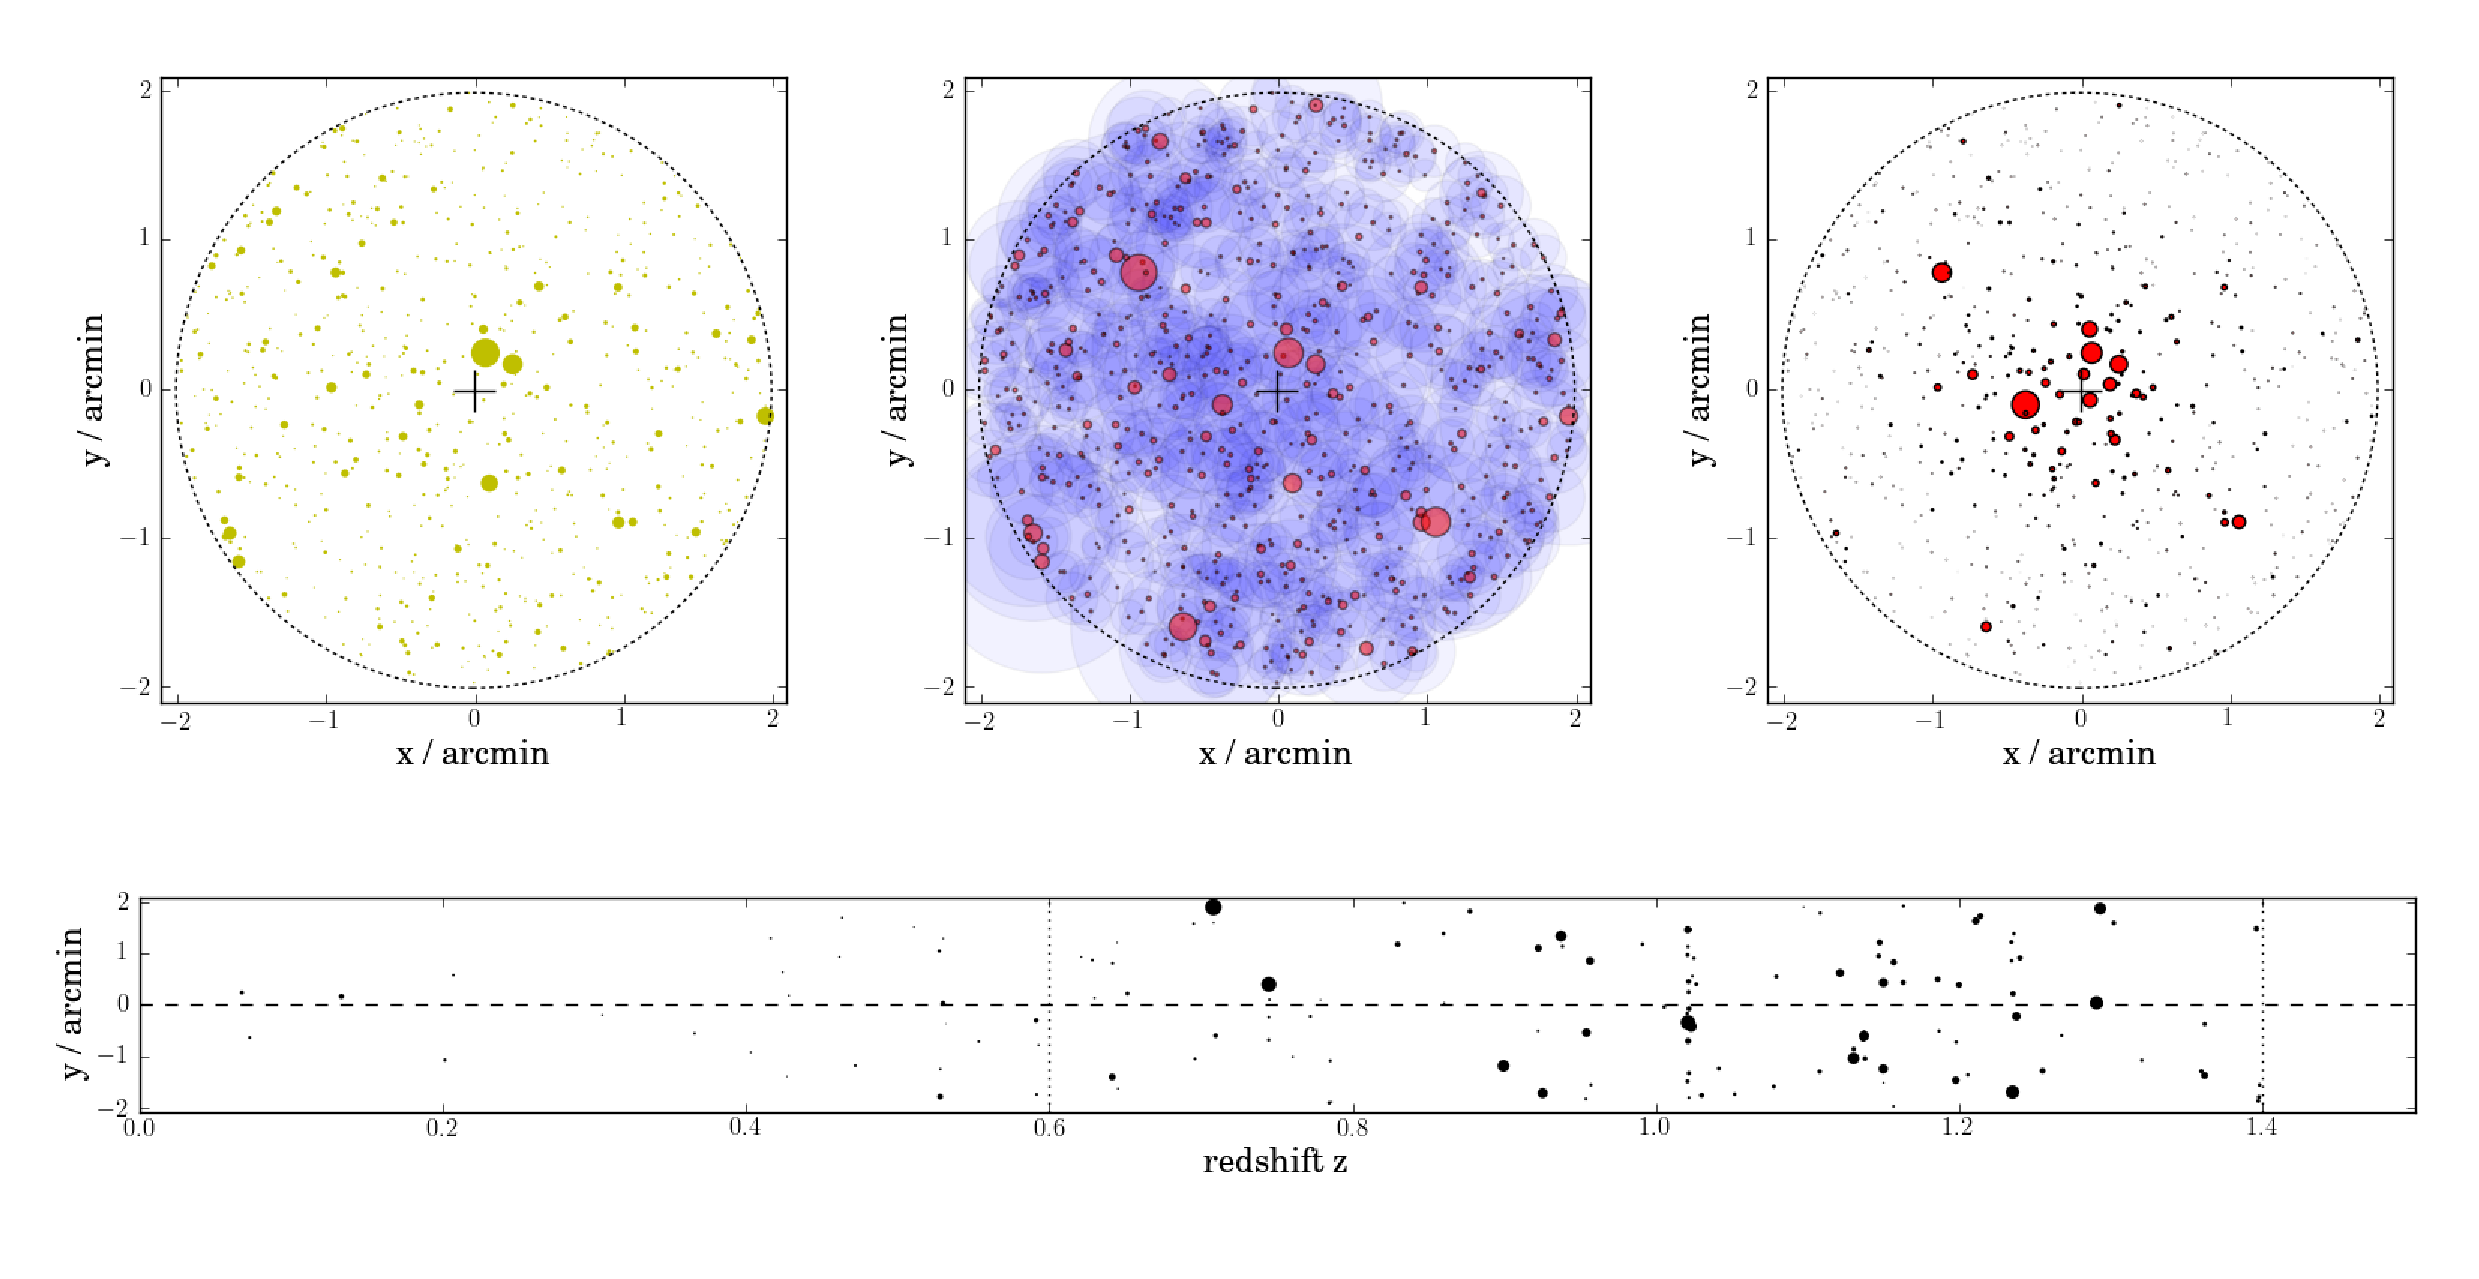
\includegraphics[width=\textwidth]{figs/viewofalightcone.eps}
\caption[magcut]{Four different views of a slightly over-dense \MS line
of sight, with a $\kappax$ of 0.03. 
{\it Top row, left:} The positions of galaxies projected on the sky. The area
of the circles is proportional to observed $i$-band flux; the brightest
object shown has an $i$ magnitude of 17.7. 
{\it Top row, centre:} The angular sizes of halos projected on the sky.
Red and blue regions lie within the NFW scale radius and virial radius
of each halo, respectively. There are essentially no empty lightcones. 
{\it Top row, right:} The individual $\kappax$ contributions of
each halo, assuming a \citet{BMO} truncated NFW 
profile and the \citet{Neto2007}
mass-concentration relation. Comparison of
this panel and the centre panel illustrates the relative importance of
proximity to the line of sight.
{\it Bottom:} A view along the redshift axis, showing only halos with
$|x|<0.3$ arcmin. The area of the points is proportional to each halo's
mass: the most massive halo shown has $1.6\times10^{12}\Msun$. The
optical axis is shown by the dashed line, while the dotted lines mark
the lens and source planes for a B1608-like strong lens.}
\label{fig:lightcone}
\end{figure*}



%%%%%%%%%%%%%%%%%%%%%%%%%%%%%%%%%%%%%%%%%%%%%%%%%%%%%%%%%%%%%%%%%%%%%%%%%%%%%%

\section{Theoretical Background}
\label{sec:theory}

\comments{
Convergence, or Ricci focusing, occurs when a gravitational lens focuses
the rays in a given bundle. This focusing can cause distant objects to
appear brighter, and larger than they would if the lens were removed.
The convergence from an isolated mass sheet is the ratio of the projected surface
mass density ($\Sigma$) \devided by the
critical surface mass density at the redshift of the mass sheet
($\Sigma_{\rm cr}$),
\be
\kappax= \frac {\Sigma}
                              {\Sigma_{\rm cr}(\zd,\zs)}
\ee
where 
\be 
\label{eq:sigcrit} 
\Sigma_{\rm cr}(\zd,\zs) \equiv \frac{c^2 D_{\rm os}}{4 \pi G D_{\rm od} D_{\rm ds}}.
\ee
and the $D$'s are the angular diameter distances between the objects
referred to in the subscripts: o is the observer, d is the deflector and
s is the source. If the surface mass density of the sheet exceeds
$\Sigma_{\rm cr}$, multiple images of the source can occur, otherwise
only one image will be observed, although that image will still be
perturbed relative to the unlensed case.


Strong lensing occurs when a massive object and background source are almost perfectly
aligned along a line of sight. The light from the background source is deflected by the
lens galaxy; this deflection allows multiple images of the background source to form
at stationary points of the time delay function. For an isolated lens, the time delay
function can be calculated from
\be \label{eq:T} 
\Delta t(\bmath{\theta},\bmath{\beta}) = \frac {1}{c} \frac{D_{\rm od} D_{\rm os}}{D_{\rm ds}} (1+z_{\rm d})\, \phi(\bmath{\theta},\bmath{\beta}),
\ee
where $\bmath{\theta}$ is the observed source position, $\bmath{\beta}$ is the 
unlensed source position, $z_{\rm d}$ is the redshift of the lens, $\phi(\bmath{\theta},\bmath{\beta})$ is
the Fermat potential. The Fermat potential is given by
\be \label{eq:FP}
\phi(\bmath{\theta},\bmath{\beta})\equiv \left[\frac{(\bmath{\theta}-\bmath{\beta})^2}{2}-\psi(\bmath{\theta}) \right], 
\ee
where $\psi(\bmath{\theta})$ is the lens potential, derived from the projected dimensionless
surface mass density, $\kappa(\bmath{\theta})$, by 
\be \label{eq:psikappa}
\kappa(\bmath{\theta})=\frac{1}{2}\nabla^2\psi(\bmath{\theta}).
\ee
}


In strong lens systems where the source is time variable, the images do not 
vary simultaneously; the optical path length for each image is different due
to relativistic and geometric effects. The difference in optical path length
causes a time-delay between the light curves of each image.
\citet{FalcoEtal1985} showed that the presence of additional matter (in the
form of a mass-sheet) along the line of sight has no observable effect except
to rescale the time-delays and magnifications. As such, it is necessary to include $\kappax$ in
the lens modelling if cosmological parameters are to be estimated accurately
and precisely from observed time delays \citep{SuyuEtal2010}. 


If there is external convergence present that is not included in the
lens modelling, then the time delay distance -- inferred assuming $\kappax
= 0$ -- will be $(1-\kappax)$ more than the true value of the time-delay distance $\Dt$:
\be 
\label{eq:MassSheet:Dtbias}
\Dt^{\rm{true}}=\frac{\Dt^{{\kappax = 0}}}{1-\kappax}.
\ee

We can hence estimate the true distance {\it only} if we have additional
knowledge of $\kappax$. Since $\kappax$ is typically small the absolute
uncertainty on the estimate of $\kappax$ corresponds to the fractional
uncertainty with which time-delay distances can be \infered.

Dynamical observations of the lens galaxy
can help break the mass-sheet degeneracy by providing an additional
estimate of the lens's mass
\citep[e.g.,][]{KoopmansEtal2003,Koopmans2004,SuyuEtal2010}. This constraint 
is useful in excluding the high convergence tails that are often present in 
PDFs for convergence - we do not include dynamical constraints in our analysis. 

In this paper we restrict ourselves to reconstructing
the line of sight portion of the mass distribution in any given field, {\it our lines of sight do not include a strong lens} which allows us to work in the weak lensing regime.  


The impact of weak-lensing perturbations on strong lensing lines-of-sight is
postponed to further work.

%%%%%%%%%%%%%%%%%%%%%%%%%%%%%%%%%%%%%%%%%%%%%%%%%%%%%%%%%%%%%%%%%%%%%%%%%%%%%%

\section{The Millennium Simulation}
\label{sec:MS}

In order to test the accuracy of our convergence estimates, we need to
know the true convergence for each line of sight. We cannot use  real
lines of sight for this,  but must use simulated lines of sight instead.
In this section we briefly review the Millennium Simulation, the ray
tracing calculations that have been carried out in it, and the mock
galaxy catalogues that have been produced.

The \MS \citep{SpringelEtal2005} is a cosmological N-body simulation of
Dark Matter structures in a cubic region approximately 680~Mpc in
co-moving size, followed from redshift 127 to the present day. With an
approximate halo mass resolution of $2\times10^{10}{\rm M}_{\odot}$
(corresponding approximately to a galaxy with luminosity $0.1L^{*}$), it
provides a detailed prediction for the distribution of dark structures
present in the Universe, under the assumptions of the $\Lambda$CDM model
of hierarchical structure formation, cosmological densities as given at
the end of \Sref{sec:intro}, and $\sigma_8 = 0.9$.
Galaxy properties,
such as stellar masses, luminosities and colours, were assigned to the
simulated halos according to a semi-analytic model for galaxy formation
\citep{DeLucia+Blaizot2007}: the resulting predictions for the galaxy
luminosity function and correlation function match the observational
data very well.

% % % % % % % % % % % % % % % % % % % % % % % % % % % % % % % % % % % % % % % 

\subsection{Convergence from Ray Tracing}
\label{sec:MS:raytracing}

\citet{HilbertEtal2009} calculated the lensing convergence using the
``lightcone'' dark matter only  output of the \MS, providing 1.7 degree
square  mock sky maps of this quantity. In this process, the dark matter
density from the simulation was projected onto a set of lens planes at
discrete redshifts, adaptively gridded and smoothed, and then the second
derivatives of the  lensing potential required for the components of the
magnification matrix were computed using a multiple lens plane ray tracing
algorithm. The first order approximation to this algorithm \citep[equation 17
of][]{HilbertEtal2009} gives the total convergence at a given sky
position~$\bmath{\theta}$ as the simple summation of the surface density in
each lens plane, weighted by the inverse critical surface density $\Sigma_{\rm
cr}$ for that plane's redshift:
\be
\kappax(\bmath{\theta}) = \sum_i \frac{\Sigma_i(\bmath{\theta})}
                                     {\Sigma_{\rm cr}(z_i,\zs)}.
\ee
\citet{HilbertEtal2009} found that this approximation is accurate to a percent level
in $\kappax$, even on 30 arcsecond scales. This accuracy sufficient for our analysis, but 
the approximation may need re-visiting in future work.

To define a test line of sight, we draw a random sky position from
within the convergence maps, bi-linearly interpolate between the pixels
of the map, and store the result as the ``true'' convergence for that
line of sight, $\kappax^{\rm true}$. 


\new{The adaptive smoothing of the matter in the \MS results in a spatial resolution of $\sim 5\,\text{kpc}$ comoving in the densest regions, and $\sim10\,\text{kpc}$ on average. This resolution is sufficient to capture most of the variance in the convergence \citep{TakahashiEtal2011}. Moreover, we seek to estimate the component of the convergence that is smooth on the angular scales of typical strong galaxy-scale lens systems ($\sim 1\,\text{arcsec}$). Any variations of the external convergence on smaller scales can be directly recovered from the resulting image distortions in the lens modelling.}


\comment{PJM: This means our sightlines are not typical of strong lenses, because they
don't include the local overdense region typically found near massive lens
galaxies. Our lines of sight have typical mass distributions for a lens line
of sight {\it after excision of the lens plane}. I have tried to explain
this above.}

% % % % % % % % % % % % % % % % % % % % % % % % % % % % % % % % % % % % % % % 

\subsection{Mock Photometric Galaxy Catalogues}
\label{sec:MS:mocks}

We construct mock photometric galaxy catalogues by selecting all \MS galaxies
within a circular aperture of a given angular radius centred on each randomly
selected line of sight position, with apparent $i$-band magnitude brighter
than a given limit. The parent catalogue, from \citet{HilbertEtal2011},
contains galaxy positions and magnitudes, all of which include lensing effects
(deflections and magnifications). We also have access to the underlying galaxy
halo masses and redshifts, which we will use to calibrate the reconstruction,
and also to explore any sources of bias and scatter. Since the ``true''
convergence is that of only the dark matter, we focus on reconstructing the
dark matter halos alone. Our model for doing this is outlined in the next
section. 

%%%%%%%%%%%%%%%%%%%%%%%%%%%%%%%%%%%%%%%%%%%%%%%%%%%%%%%%%%%%%%%%%%%%%%%%%%%%%%

\section{Estimating Convergence: The Halo Model Approximation}
\label{sec:model}

We require a method for estimating the convergence at any point on the sky,
given a catalogue of observed galaxy properties such as positions,
brightnesses, colours, and possibly stellar masses and redshifts, for every
galaxy in the field of the lens, down to some magnitude limit. Since we cannot
observe the surface mass density of each halo directly, we need some way of
estimating the mass of each halo in the catalogue, so that we can compute its
contribution to the total $\kappax$ along the line of sight \citep[as in
\eg][]{GunnarssonEtal2006,KarpenkaEtal2012}.  This mass
assignment recipe will be uncertain, and also incomplete, but it can be
calibrated with cosmological simulations, which represent a significant
additional source of information to what is present in the data.

Transforming an observed photometric galaxy catalogue into a  catalogue of
halo masses, positions, and redshifts will enable us to attempt a
reconstruction of the convergence induced by every halo near a line of sight. 
We also need to account for the convergence due to dark structures and the
divergence due to voids; we do not model voids or dark structures, but their
effects are included statistically by calibrating the convergence in
halos, $\kappah$, against the ray-traced convergence, $\kappax$, for \MS lines
of sight.


% % % % % % % % % % % % % % % % % % % % % % % % % % % % % % % % % % % % % % % 

\subsection{Halos}
\label{sec:model:halos}

Cosmological dark matter simulations have shown that dark matter
halos are reasonably well-approximated by NFW profiles 
\citep{NFW}. We assume each halo to have a spherical mass distribution with 
density given by
\be\label{eq:rhonfw}
\rho(r) = 
\frac{\rho_0}{\left(r/r_{s}\right)
\left(1+r/r_{s}\right)^{2}}.
\ee
Here, $r_{s}$ is a characteristic scale 
radius of the cluster, representing the point where
the density slope transitions from $r^{-1}$ to $r^{-3}$. This radius is
related to the virial radius of the halo by $r_{s}~=~r_{200}/c$, where $c$ is
the concentration parameter, which can be estimated from the halo's mass,
using a mass--concentration relation. Typically more massive halos are less
concentrated, but there is some scatter; we use the relation of
\citet{Neto2007} to estimate $c$ from the mass enclosed within $r_{200}$,
which we denote as $M_{200}$. We find our results do not change if the
\citet{MaccioEtal2008} mass--concentration relation is used instead. 

If one integrates the density profile of an NFW profile out to infinite
radius, the total mass diverges. Similarly, if the universe is
homogeneously populated with NFW halos, the projected surface mass along
any line of sight will also be divergent.\footnote{At large radius,
$\Sigma_{\rm nfw} \propto R^{-2}$, but the differential number of halos
centred within an annulus of width $\dee R$ is given by $\dee N_{\rm
annulus} \propto R \dee R$, so  $\Sigma_{\rm total} \propto
\int_{0}^{\infty} R^{-1} \dee R$, which diverges logarithmically} Since
infinite mass is unphysical, the profile must be truncated at some
point. Several truncation profiles have been suggested
\citep[e.g][]{BMO}, but beyond several virial radii, the amount of
matter associated with a halo is likely to be low. In this work we
assume the truncated NFW profile
\be\label{eq:bmoprofile}
\rho(r) = 
\frac{\rho_{\rm NFW} (r)}{1+\left(r/r_{t}\right)^2},
\ee
which is the same as the NFW profile in the limit that the truncation
radius, $r_t$ goes to infinity; the shear and convergence from such a
profile are derived in \citet{BMO}.
 We use a truncation radius of five times
the virial radius, but our results are robust for any choice of $r_t>2
\times r_{200}$. 

Many studies have shown that galaxies have total mass density profiles that
are approximately isothermal in their inner regions
\citep[\eg][]{AugerEtal2010} due to the more concentrated stellar mass
component.
This has been confirmed by galaxy-galaxy weak lensing measurements 
\citep[\eg][]{Mandelbaum,GavazziEtal2007}. We note that the two halo term that
dominates the galaxy-galaxy lensing signal at large radii is explicitly taken
into account in our model, where every galaxy is assigned a dark matter halo.
At large radii an NFW-like profile is probably appropriate, but may not be
correct when a halo is very close to the line of sight.


Each halo in our catalogue contributes to
the line of sight convergence by
\be
\label{eq:kappai}
\kappa_i =\Sigma_{i}/\Sigma_{\mathrm{cr}}(z_i,\zs),
\ee
where $\Sigma_{\mathrm{cr}}(z_i,\zs)$ is the critical surface density \comments{was defined in \Eref{eq:sigcrit}}.
Following the first order approximation of \citet{HilbertEtal2009}
outlined in \Sref{sec:MS} above, we compute 
the total convergence from all the halos along the line
of sight using
\be 
\label{eq:kappasummu}
\kappah = \sum_{i} \kappa_i.
\ee

To estimate a halo's contribution to $\kappah$ we must first know the
halo's mass \new{and position. The stellar mass
and host halo are not necessarily concentric, especially for central
galaxies of giant clusters, but our reconstruction assumes the dark matter halo is centred on
the visible galaxy.} For the lines of sight of the \MS, halo masses are
known, but for  real lines of sight the halo masses have to be \infered
from whatever data are available. 
In this work we investigate the use of the empirical stellar mass --
halo mass relation for this purpose. The primary advantage of this
approach is that it is a simple, ``one size fits all'' relation that can
be applied regardless of the stellar mass observed. We discuss
additional observables that could be used to improve the precision of
the halo mass inference in \Sref{sec:discuss} below. 

We use the relation of \citet{BehrooziEtal2010} to infer halo masses
from stellar masses; the details of this \proceedure are outlined in 
\Aref{appendix:MSMH}. Given an uncertain stellar mass and redshift for
each galaxy in the  catalogue, we draw a sample halo mass from the PDF
that describes this uncertainty (\Eref{eq:mhalo-mstar}) and use
\Eref{eq:kappai} to compute its contribution to the convergence,
$\kappa_i$; this can be done for all the halos along a specific line of sight
and summed to give a sample value of $\kappah$;  repeatedly applying
this \proceedure allows us to build up a histogram of $\kappah$ values
consistent with the data, and hence characterize $\pr(\kappah|\data)$. 

This PDF contains a hidden assumption of an uninformative prior PDF for
$\kappah$ -- in the case of infinitely poorly measured stellar masses and
redshifts, $\pr(\kappah|\data)$ will have very long tails corresponding to
very over-dense lines of sight that we do not believe exist. The resolution of this
is to divide out the effective prior PDF that was applied during the halo mass
estimation process (which is broad, and hence close to uniform), and apply an
additional prior on $\kappah$, given by the global underlying $\kappah$
distribution from the simulation. In the limiting  case of very poor
photometric data, $\pr(\kappah|\data)$ then defaults to this distribution, as
required.

% \todo{All}{Discuss this. It ties us to the simulation, but only weakly. Is the
% argument about poor data valid? Tom?}

% TEC: yes it's valid. It only really ties us to the halo mass function of the
% simulation. It's probably tied at the same level as the "global P(\kappa) as
% derived from Stefan's ray-tracing"


% % % % % % % % % % % % % % % % % % % % % % % % % % % % % % % % % % % % % % % 

\subsection{Accounting for voids, filaments and other dark structures}
\label{sec:model:voids}

Our halo model accounts for the convergence contribution of density
perturbations that can be associated with light. Filaments and dark
substructures contribute additional convergence, while voids contribute a
divergence; these structures must be included to produce an unbiased estimate
of $\kappax$. In particular, neglecting voids would lead to a heavily biased
estimate of $\kappax$, since the halo model's $\kappah$ can only be positive.
In principle the absence of galaxies implies something about the presence of a
void, but we do not currently attempt to use this information. In general, it
is difficult to account for the unseen mass, since we do not have a good model
for its density structure.

The solution we present here is to calibrate the relationship between the halo
convergence $\kappah$ and the overall convergence $\kappax$ (as would be
calculated by ray tracing through the full density field)  using the
simulations themselves. The halo modelling procedure outlined in
\Sref{sec:model:halos} allows  us to estimate  the convergence due to halos
given observations of  mass, redshift and position,
$\pr(\kappah|\data)$, but what we are interested in is the total
convergence along the line of sight $\pr(\kappax|\data)$. We can obtain
this by considering the expression: 
\begin{equation} 
\Pr(\kappax|\data) = 
   \int \dee\kappah  \Pr(\kappax|\kappah,\data) \Pr(\kappah|\data)
   \label{eq:kappaconv}
\end{equation} 
The first term in the integrand relates the convergence due to model halos,
$\kappah$, to the true convergence, $\kappax$. This conditional distribution
can be constructed from the \MS catalogues, by computing
$\kappah$ from the true halo masses and redshifts 
along each selected line of sight, and then
accumulating $\kappah$, $\kappax$ pairs
for a large number of such sightlines. 
For any given line of sight we can then estimate
$\pr(\kappah|\data)$ as described above, and then multiply it by
$\Pr(\kappax|\kappah)$ and integrate out the intermediate parameter
$\kappah$. 

\phil{However, if the conversion between stellar mass and halo mass is very
uncertain, $\pr(\kappah|\data)$ is shifted relative to what it would
have been given perfect knowledge of the halo masses.  This is because the
conversion from stellar mass to halo mass and into $\kappah$ is highly
asymmetric: a long tail of high halo masses gives rise to a tendency to
overestimate $\kappah$. If this shift is ignored, the resulting
$\Pr(\kappax|\data)$ will be systematically biased towards high values of
$\kappax$. Instead, we need the  distribution of $\kappax$ from all
calibration lines of sight that have a $\pr(\kappah|\data)$ that is identical
to the $\pr(\kappah|\data)$ for the real line of sight {\it given the same
data quality}; however, we found this approach unfeasible  given our finite
number of calibration lines of sight. A working compromise is to use 
the median of the $\pr(\kappah|\data)$ distributions in the calibration.}

We  take a large number of
calibration lines of sight from the \MS catalogues and generate a mock
stellar mass catalogue for each one. We then reconstruct each lightcone in the
same way as we would an observed field,
estimate $\pr(\kappah|\data)$, and extract its median. Accumulating
these median values $\kappah^{\rm med}$ and 
their corresponding true values of $\kappax$, we can form the 
conditional distribution $\pr(\kappax|\kappah^{\rm med})$. 
Then, to infer $\kappax$ from an observed photometric catalogue, we 
estimate $\pr(\kappah|\data)$ 
using the halo model, compute the median value 
$\kappa_{\rm h,obs}^{\rm med}$, and then use a modified
version of 
\Eref{eq:kappaconv} to infer $\kappax$: 
\bea
\Pr(\kappax|\kappah^{\rm med},\data) &=& \int \dee\kappah^{\rm med} 
   \Pr(\kappax|\kappah^{\rm med},\data) \Pr(\kappah^{\rm med}|\data) \notag \\
\label{eq:calkappaconv}   
\eea
\phil{This integral is trivial, since $\Pr(\kappah^{\rm med}|\data)$ is
a delta function centred on the median of the inferred PDF for $\kappah$.
However,}
because we only have a finite number of calibration lines of sight, we use all
calibration lines of sight with $\kappa_{\rm h,cal}^{\rm med} =
\kappah^{\rm med}\pm0.003$ to form $\Pr(\kappax|\kappah^{\rm
med},\data)$.
\comments{, with each calibration sightline weighted equally. PJM: why is
this? Surely one should weight by the value of the Gaussian function implied
by that ``$\pm 0.003$''?}

This procedure of reducing the full PDF for $\kappah$ to its median increases
the importance of the realism of the simulation: the simulation needs to be as
similar as possible to the real universe or there is a possibility of
systematic errors. Conversely, making use of all the information
in the photometric catalogue yields $\kappax$ estimates of increased
precision.

%%%%%%%%%%%%%%%%%%%%%%%%%%%%%%%%%%%%%%%%%%%%%%%%%%%%%%%%%%%%%%%%%%%%%%%%%%%%%%

\section{Results: Perfect Halo Data}
\label{sec:knownMh+z} 

We now put the reconstruction \proceedure outlined above into practice, first
inferring $\kappax$ from $\kappah$ in the case of hypothetical galaxy
catalogues with noiseless redshifts and halo masses. The reason for doing this
is to check the validity of the calibration process, and then also to 
investigate the primary sources of the convergence. It will also provide us
with a measure of the intrinsic uncertainty introduced by our assumptions of
all illuminated halos being spherically-symmetric truncated NFW halos following the
Neto et al concentration--mass relation \new{and of visible galaxies being concentric with their host halos}.

% % % % % % % % % % % % % % % % % % % % % % % % % % % % % % % % % % % % % % % 

\subsection{How is $\kappah$ related to $\kappax$?}

\Fref{fig:jointkh-k} shows the conditional distribution of $\kappax$ given 
$\kappah$, derived from $10^5$ randomly selected \MS lines of sight
and assuming noise-free halo masses and redshifts. 
\phil{In this case, $\pr(\kappah|\data)$ is almost a delta function since the only uncertainty is halo
concentration, which has minimal effect on $\pr(\kappah|\data)$.  
}
% In this case, the PDF : we can read
% off  $\pr(\kappax|\data)$ just by taking a thin vertical slice through this 
% distribution. 
% Note that the joint PDF plotted in this figure is the product
% of  the conditional distribution that we need for calibration, and also the
% prior PDF for $\kappah$ that we need to ensure that the global distribution of
% $\kappah$ values is defaulted to in the case of poor observational data. 
At fixed $\kappah$ we find in \Fref{fig:jointkh-k} that the scatter in 
$\kappax$
grows with $\kappah$; our reconstruction is better at reproducing under-dense
lines of sight than over-dense lines of sight. The effect of ignoring voids
and the smooth mass component is evident in this plot: $\kappah$ is
significantly higher than $\kappax$, at any given $\kappax$ value. 
\phil{Conditioning on $\kappah$ gives a PDF for
$\kappax$ centred at the correct place, by construction.}

%%%%%%%%%%%%%%%%%%%%%%%%%%%%%%%%%%%%
\begin{figure}
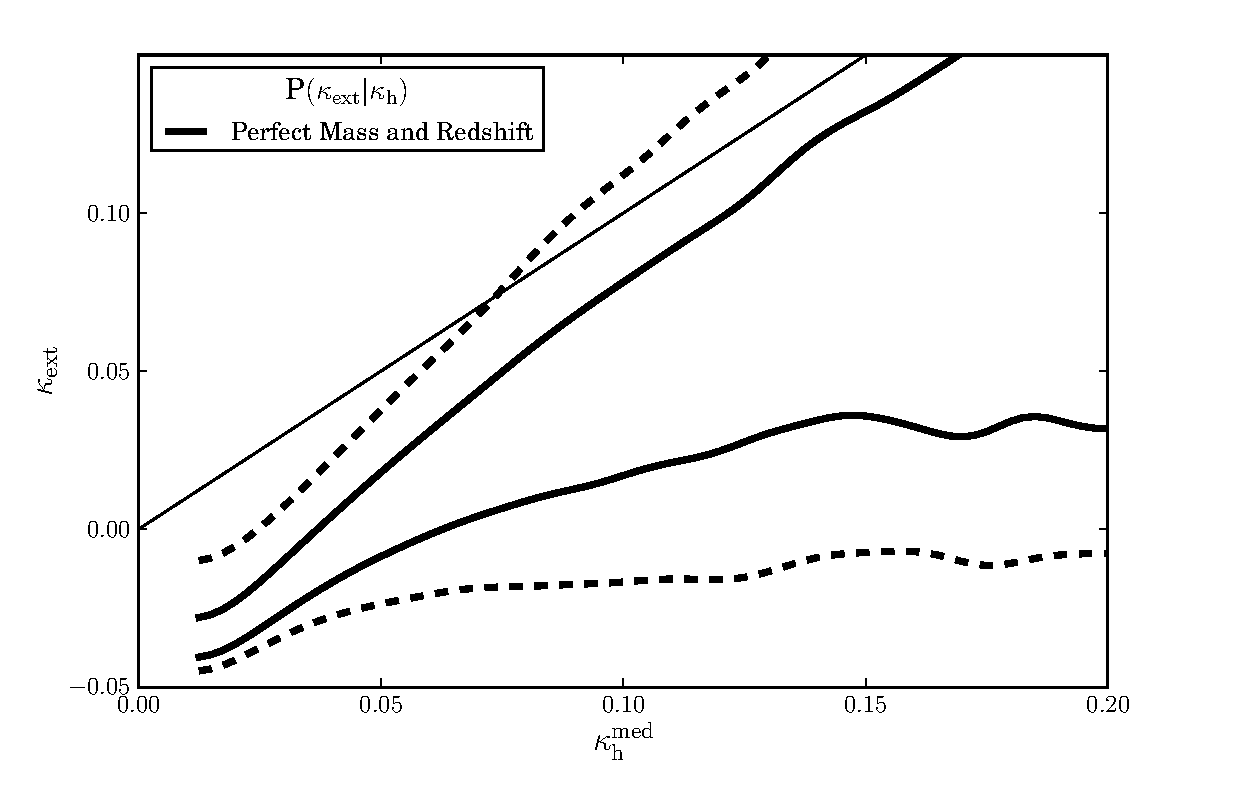
\includegraphics[width=\columnwidth]{figs/cornerplot.eps}
\caption[Biased?]{The conditional distribution of 
$\kappax$ given $\kappah$, in the case where  
we have perfect knowledge of halo mass and redshift.
$10^5$ reconstructed lines of
sight were used to make this plot. 
Solid (dashed) lines enclose 68\% (95\%) of the conditional probability.
$\kappah$ traces $\kappax$, but with a positive offset which arises from
$\kappah$ not accounting for any voids or dark structures.
At fixed $\kappah$ the scatter in $\kappax$ grows rapidly with $\kappah$.
\tom{The thin diagonal line follows $\kappax=\kappah$.}}
\label{fig:jointkh-k}
\end{figure}
%%%%%%%%%%%%%%%%%%%%%%%%%%%%%%%%%%%%


% % % % % % % % % % % % % % % % % % % % % % % % % % % % % % % % % % % % % % % 

\subsection{How accurate is the $\kappah - \kappax$ calibration?}

%%%%%%%%%%%%%%%%%%%%%%%%%%%%%%%%%%%%
\begin{figure}
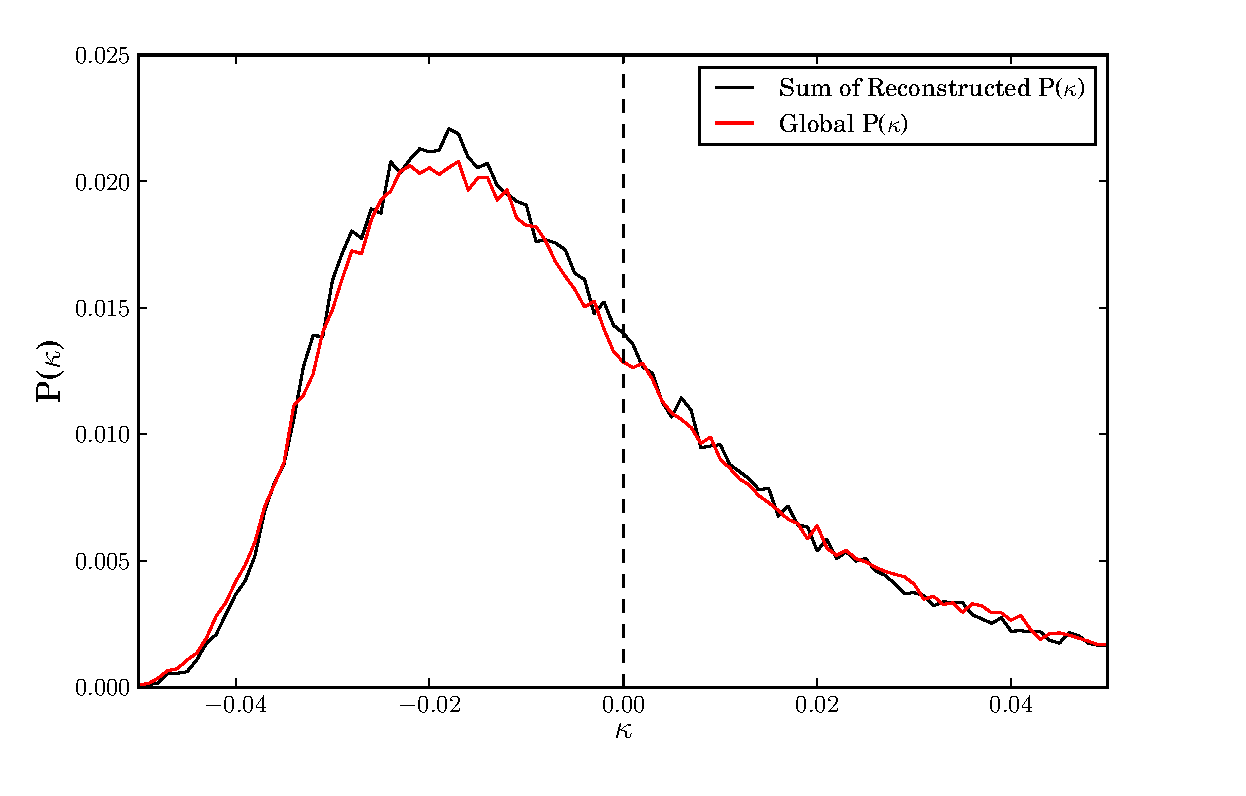
\includegraphics[width=\columnwidth]{figs/globaldist.eps}
\caption[magcut]{Recovering the global $\pr(\kappax)$ (shown in red). The
black curve shows a histogram of  inferred  $\kappax$ values from $10^{5}$
reconstructed lines of sight.  The reconstructions were performed given
perfect knowledge of halo mass and redshift -- in this case the reconstruction
recovers the correct convergence.}
\label{fig:globaldist}
\end{figure}
%%%%%%%%%%%%%%%%%%%%%%%%%%%%%%%%%%%%

%%%%%%%%%%%%%%%%%%%%%%%%%%%%%%%%%%%%
\begin{figure*}
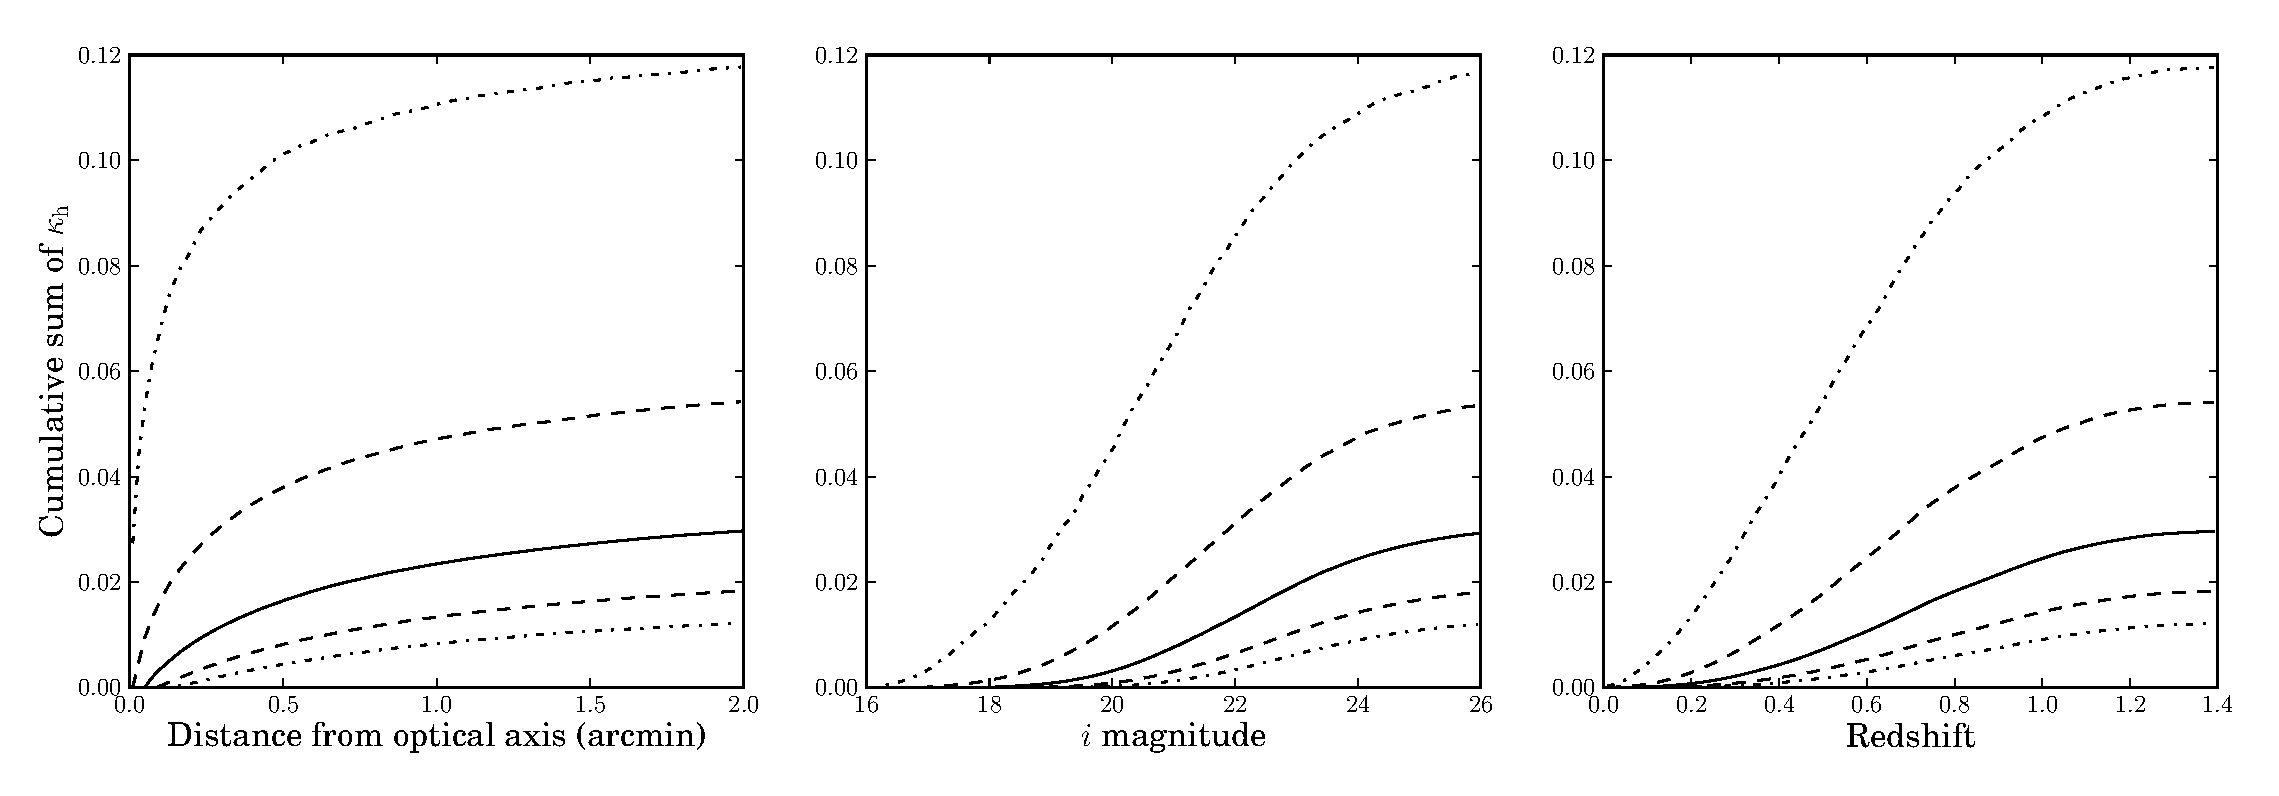
\includegraphics[width=\textwidth]{figs/where_is_the_kappa.eps}
\caption[magcut]{Which objects dominate the external convergence for a line of
sight? From left to right, the three figures show the cumulative contribution
to the total convergence from individual halos ($\kappah$) as a function of
1) distance from the line of sight, 2) magnitude and 3) redshift.   In each
panel, the solid line is the median cumulative contribution over a large
sample of lines of sight, while dashed and dot-dashed show the ranges enclosing 68
and 95 percent of the lines of sight respectively. The source is at redshift 1.4.}
\label{fig:where}
\end{figure*}
%%%%%%%%%%%%%%%%%%%%%%%%%%%%%%%%%%%%

Let us define the ``bias'' of the reconstruction of a given line of sight as
the difference between the expectation value of $\kappax$ over its posterior
PDF $\pr(\kappax|\data)$ and the known true value $\kappax^{\mathrm{true}}$.
Let us also define the ``width,'' $\sigma_{\kappa}$, to be half the width of
the interval containing the central $68\%$ of the posterior probability
$\pr(\kappax|\data)$. 

In an ensemble of $10^{5}$ reconstructed lines of sight, we find the mean bias
to be $-1\times 10^{-5}$, and the mean width to be 0.01. This is
1.8 times smaller than the width of the global $\pr(\kappax)$.  We find that
our inferred $\kappax$ PDFs are consistent with the global $\kappax$
distribution; \Fref{fig:globaldist} shows that sampling from the
$\pr(\kappax|\data)$ inferred from reconstructions of  $10^{5}$ lines of
sight  produces a distribution of $\kappax$ values over the sky nearly identical to
the global $\pr(\kappax)$. Given perfect knowledge of halo mass and redshift
then, the calibration \proceedure provides an unbiased estimate of $\kappax$
that is $1.8$ times more precise than using the global $\pr(\kappax)$. 
\phil{This is the maximum precision we can obtain using the current calibrated
halo model.}

% % % % % % % % % % % % % % % % % % % % % % % % % % % % % % % % % % % % % % % 

\subsection{Which halos dominate the $\kappah$ distribution?}

Before investigating the impact of imperfect knowledge of halo
mass and redshift, we investigate the uncertainties induced by limits on the
magnitude of the observed galaxy sample, and on the field of view. The halos
in our catalogue are populated by galaxies and given magnitudes according to
the semi-analytic model of \citet{DeLucia+Blaizot2007}: by applying magnitude
cuts to our catalogue, we can investigate the amount of scatter caused by
unobserved halos. 

\Fref{fig:where} shows the cumulative contribution to $\kappah$ as a function
of projected distance from the line of sight, magnitude and redshift. We find
that most of the convergence comes from halos close to the line of sight. 
Over half of the  convergence typically comes from halos within 30 arcseconds
of the line of sight; by 2 arcminutes, this fraction is 85\%. The contribution
from halos beyond 2 arcminutes is relatively constant at a contribution of
0.008$\pm$0.003. We find that ignoring halos beyond 2 arcminutes has no effect
on the precision of the reconstruction; this is shown in \Fref{fig:radcut}. As
a function of magnitude, we find that $\kappah$ is dominated by objects with
magnitudes between $i=18$ and $i=24$. Objects brighter than $i=18$ are either
too rare, or too close to the observer, to make a significant contribution to
the convergence. Objects fainter than $i=24$ are too small to be important,
unless they are extremely close to the line of sight; we find that
including halos fainter than $i=24$ does not improve the reconstruction. 
\Fref{fig:magcut} shows the scatter on $\kappah-\kappax$ (where $\kappah$ is
shifted so that its mean is zero, \phil{to emulate the effect of the eventual
calibration}) as a function of reconstruction magnitude limit. We do not
expect a deeper survey to decrease the size of the uncertainty in mapping
$\kappah$ onto $\kappax$. Halos at all redshifts out to the source redshift
(1.4 in this work. The redshift of the source in B1608+656) contribute to the convergence, but the largest contribution comes
from halos with $z \sim z_{\rm source}/2$.

%%%%%%%%%%%%%%%%%%%%%%%%%%%%%
\begin{figure}
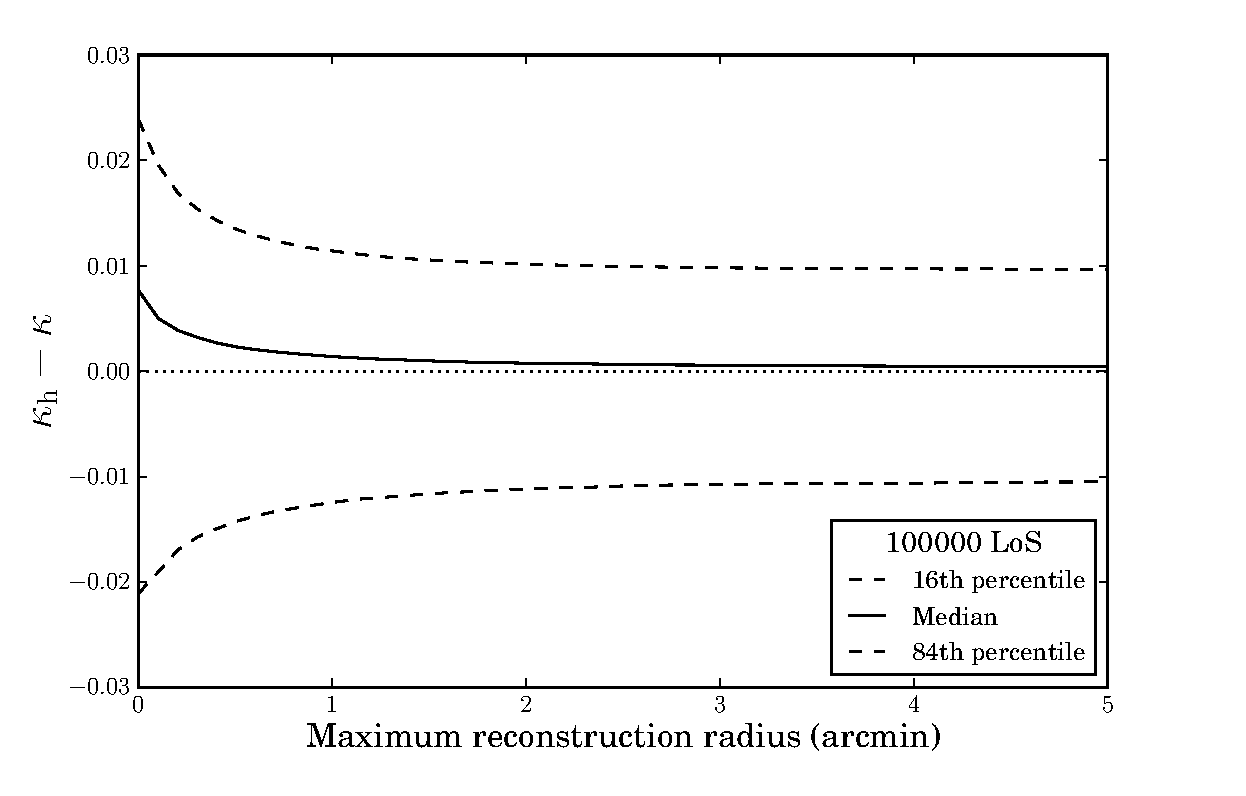
\includegraphics[width=\columnwidth]{figs/radius_scatter.eps}
\caption[magcut]{The 16, 50 and 84th percentiles of $\kappah$ minus
$\kappax$ as a function of the limiting radius of the halo
reconstruction. $\kappah$ has been shifted such that
$\left\langle\kappah\right\rangle=0$ \phil{to emulate the effect of the
eventual calibration}. 
The majority of the constraining power
comes from reconstructing halos within 2~arcmin of the line of sight.}
\label{fig:radcut}
\end{figure}
%%%%%%%%%%%%%%%%%%%%%%%%%%%%%

%%%%%%%%%%%%%%%%%%%%%%%%%%%%%
\begin{figure}
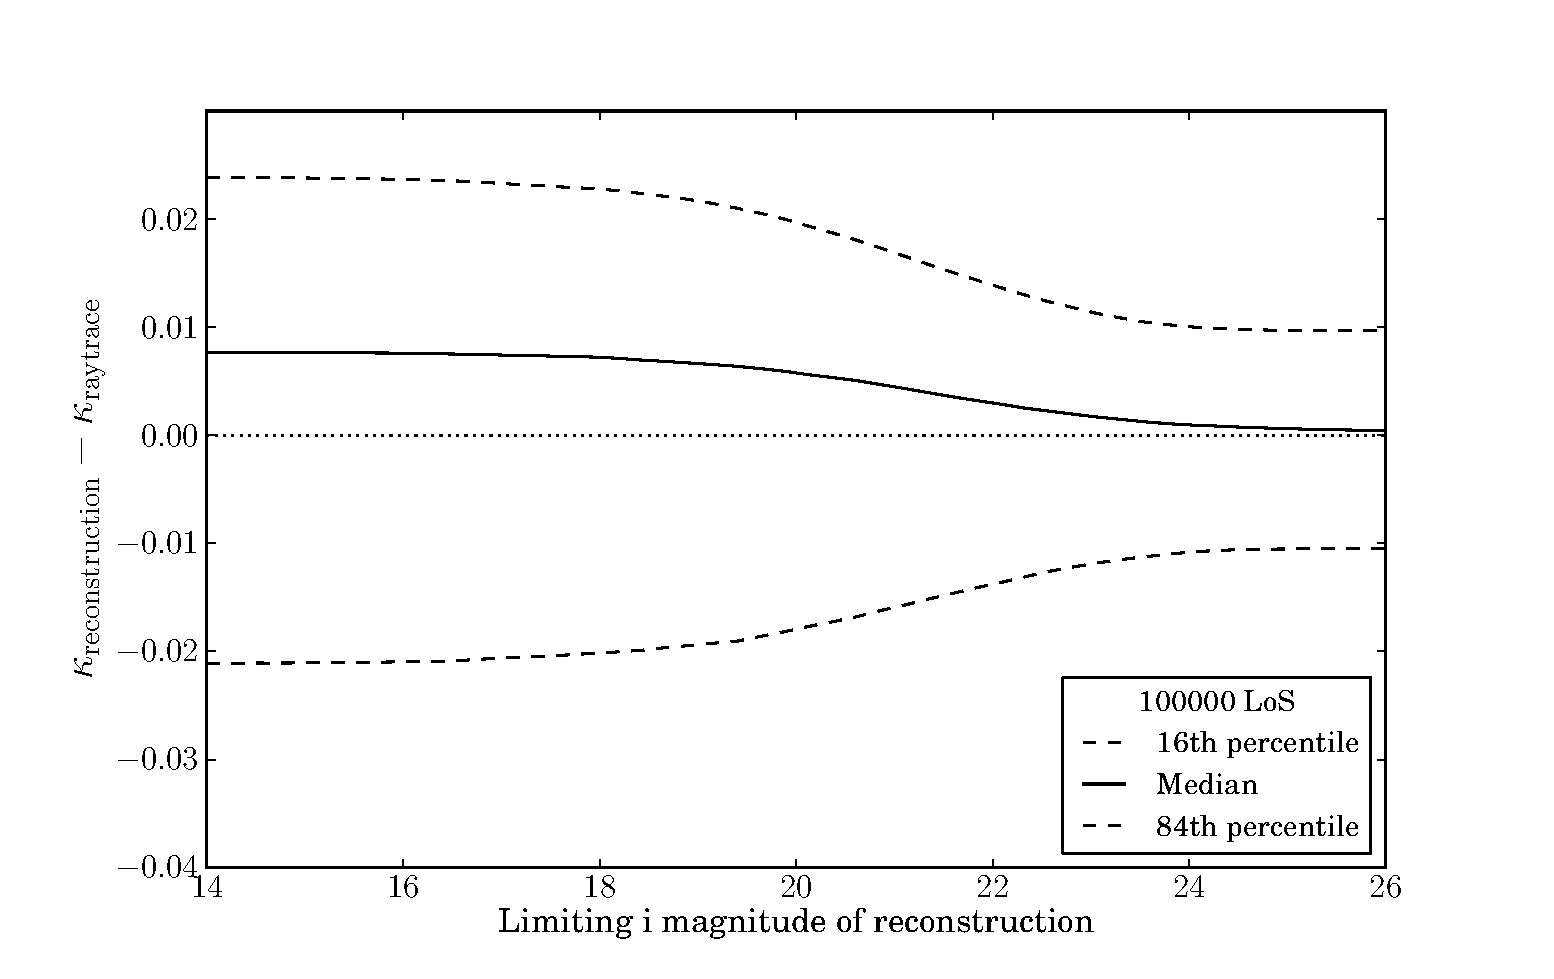
\includegraphics[width=\columnwidth]{figs/mag_scatter.eps}
\caption[magcut]{The 16, 50 and 84th percentiles of $\kappah$ minus
$\kappax$ as a function of the limiting $i$ band depth of the halo
reconstruction. $\kappah$ has been shifted such that
$\left\langle\kappah\right\rangle=0$ \phil{to emulate the effect of the
eventual calibration}. The majority of the constraining power
comes from reconstructing halos with magnitudes between $18<i<24$.}
\label{fig:magcut}
\end{figure}
%%%%%%%%%%%%%%%%%%%%%%%%%%%%%


%%%%%%%%%%%%%%%%%%%%%%%%%%%%%%%%%%%%%%%%%%%%%%%%%%%%%%%%%%%%%%%%%%%%%%%%%%%%%%%%

\section{Testing the Halo Model Reconstruction on Mock Galaxy Catalogues}
\label{sec:obsMstar+z}

We now move on to consider the halo model reconstruction of line-of-sight mass
distributions given noisy astronomical observables. A typical imaging survey
can be expected to provide measurements of the positions and magnitudes of
galaxies in a field;  spectra for some of the objects may either come from a
synergistic survey, or from targeted follow-up. In this section we quantify
the uncertainties induced by inferring the halo mass and redshift from these
observables. 

%\flag{Should we show the relevant calibration plots, analogous to Figure 2?
%Seems a bit odd to give Figure 2 but not illustrate the {\it actual
%calibration procedure we follow on real data}... Maybe we could make one that
%had the conditional distribution for each data quality?}

%TEC: I think that could lead to figure overload; the concept is given throughout
% the paper, and it's well illustrated by figure 2.

As described in \Sref{sec:model:halos}, in this work we attempt to  infer halo
masses from measurements of stellar mass. We will investigate two main sources
of uncertainty: the stellar masses themselves, and placing halos at
photometric redshifts. Much work has already focused on using photometric
colours to infer stellar mass \citep[\eg][]{AugerEtal2009} and redshifts
\citep[\eg][]{BPZ}: we will estimate the likely uncertainties on stellar mass
and redshift based on this work.  


% % % % % % % % % % % % % % % % % % % % % % % % % % % % % % % % % % % % % % % 

\subsection{Making Mock Observational Catalogues}

\phil{While the \MS catalogues do already contain stellar masses for each
galaxy, we do not use them for two reasons. The first is that at the low mass
end, the dark matter-only \MS satellite galaxy halos are highly  stripped
relative to what we might expect in a universe containing baryons, leading to
a mismatch between the observed and simulated stellar mass--halo mass
relations.  The second is that we wanted to be able to perform the functional
test of trying to recover the convergence having assumed the correct stellar
mass--halo mass relation.} For these reasons, we assign a new true stellar
mass to each halo in the \MS catalogues, according to the empirical stellar
mass--halo mass relation of \citet{BehrooziEtal2010}. \new{When assigning stellar
masses we have treated satellites in the same way as central halos; in the real
universe both the density profile and the stellar mass--halo mass relation are
likely different for satellites and centrals, but our simple model does not include
these effects}. From these we simulate
observed stellar masses by drawing samples from  $\pr(\log{M^{*}_{\rm
obs}}|\log{M^{*}_{\rm true}})$ which we take to be a Gaussian of width
$\sigma_{M_*}$ centred on $\log(M*_{\mathrm {true}})$. Where a spectroscopic
redshift exists, stellar masses can be estimated with typical uncertainties of
0.15 dex \citep{AugerEtal2009}; however with photometric redshifts stellar
mass uncertainties are typically three times as large. We use
$\sigma_{M_*}=0.15$ dex for halos with a spectroscopic redshift and
$\sigma_{M_*}=0.45$ dex otherwise. For photometric redshift uncertainties we
draw a redshift from $\pr(z_{\rm true}|z_{\rm obs})$ which we take to be a
Gaussian of width $0.1(1+z_{\rm spec})$ centred on $z_{\rm spec}$, where
$z_{\rm spec}$ is the halo's true redshift in the \MS catalogue. \new{In our mock catalogues 
we have used the galaxy position from the \MS; this is not necessarily coincident with the
centre of the galaxy's host dark matter halo.}

\comment{The following is relevant to all sections on inferring $\kappax$
given imperfect data, so it belongs here and not in the spectroscopic redshift
first subsection.}

Given an uncertain stellar mass and redshift it is possible to infer a
halo mass using the stellar mass--halo mass relation of
\citet{BehrooziEtal2010}. This \proceedure requires an inversion of the
relation given in \citet{BehrooziEtal2010} and correctly inverting the
relation's uncertainties requires care: the \proceedure we use to do this
is given in \Aref{appendix:MSMH}. By drawing sample halo masses
and redshifts, we can infer a sample $\kappah$ using the \proceedure of
\Sref{sec:model}. Repeatedly drawing samples allows us to
estimate $\pr(\kappah|\data)$ for each reconstructed line of sight. We then
transform this into our target PDF $\pr(\kappax|\data)$ as described above.


% % % % % % % % % % % % % % % % % % % % % % % % % % % % % % % % % % % % % % % 

\subsection{Reconstructing $\kappax$ given a spectroscopic redshift for every object}

%%%%%%%%%%%%%%%%%%%%%%%%%
\begin{figure}
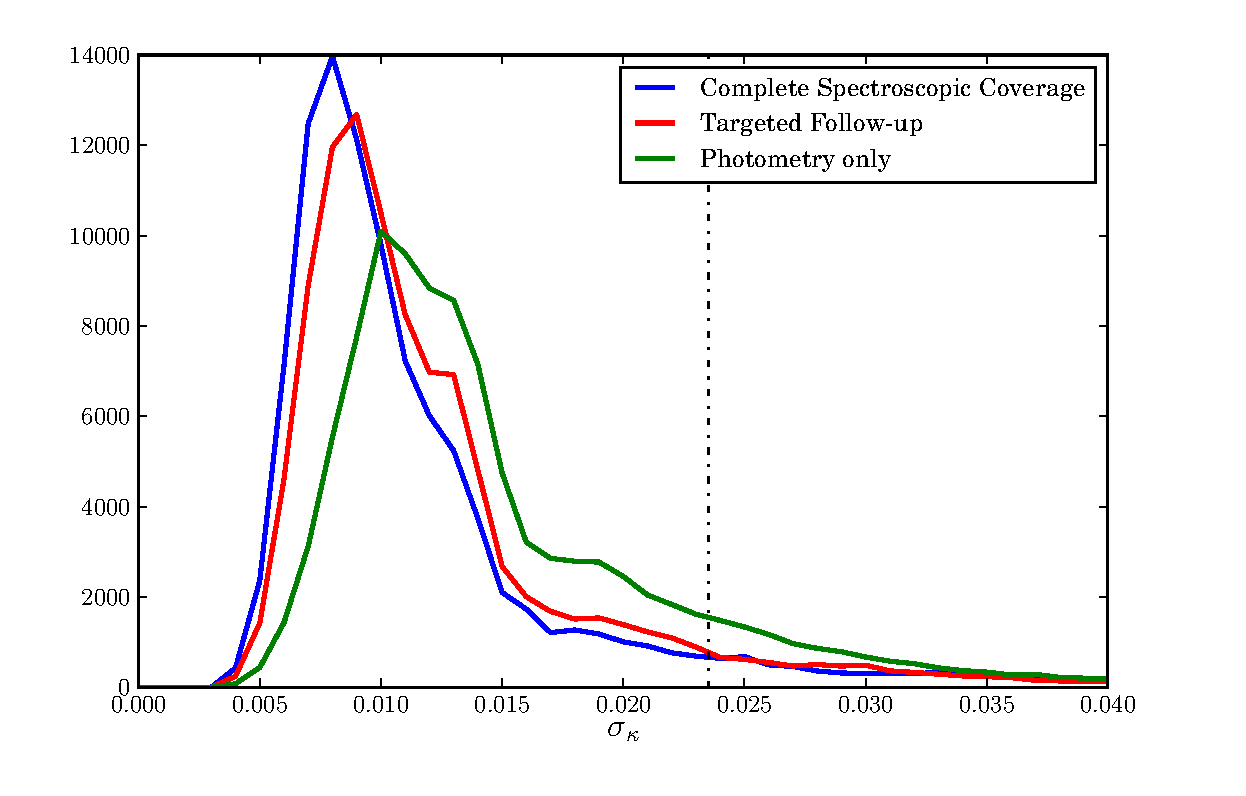
\includegraphics[width=\columnwidth]{figs/Width.eps}
\caption{The widths of the \infered PDFs $\pr(\kappax|\data)$ for
$10^5$ lines of sight, given different quality of data. 
Blue: spectroscopic redshift for every halo with $i<26$; 
Red: spectroscopic redshift for every halo with $i<23$, 
and every halo with $i<24$ within 1 arcminute, while all other objects just
have photometric redshifts;
Green: all the objects in the field have only photometric redshifts. The
vertical dot-dashed line marks the width of the global $\pr(\kappax)$ for all
lines of sight.}
\label{fig:reconwidths}
\end{figure}
%%%%%%%%%%%%%%%%%%%%%%%%%

%%%%%%%%%%%%%%%%%%%%%%%%%
\begin{figure}
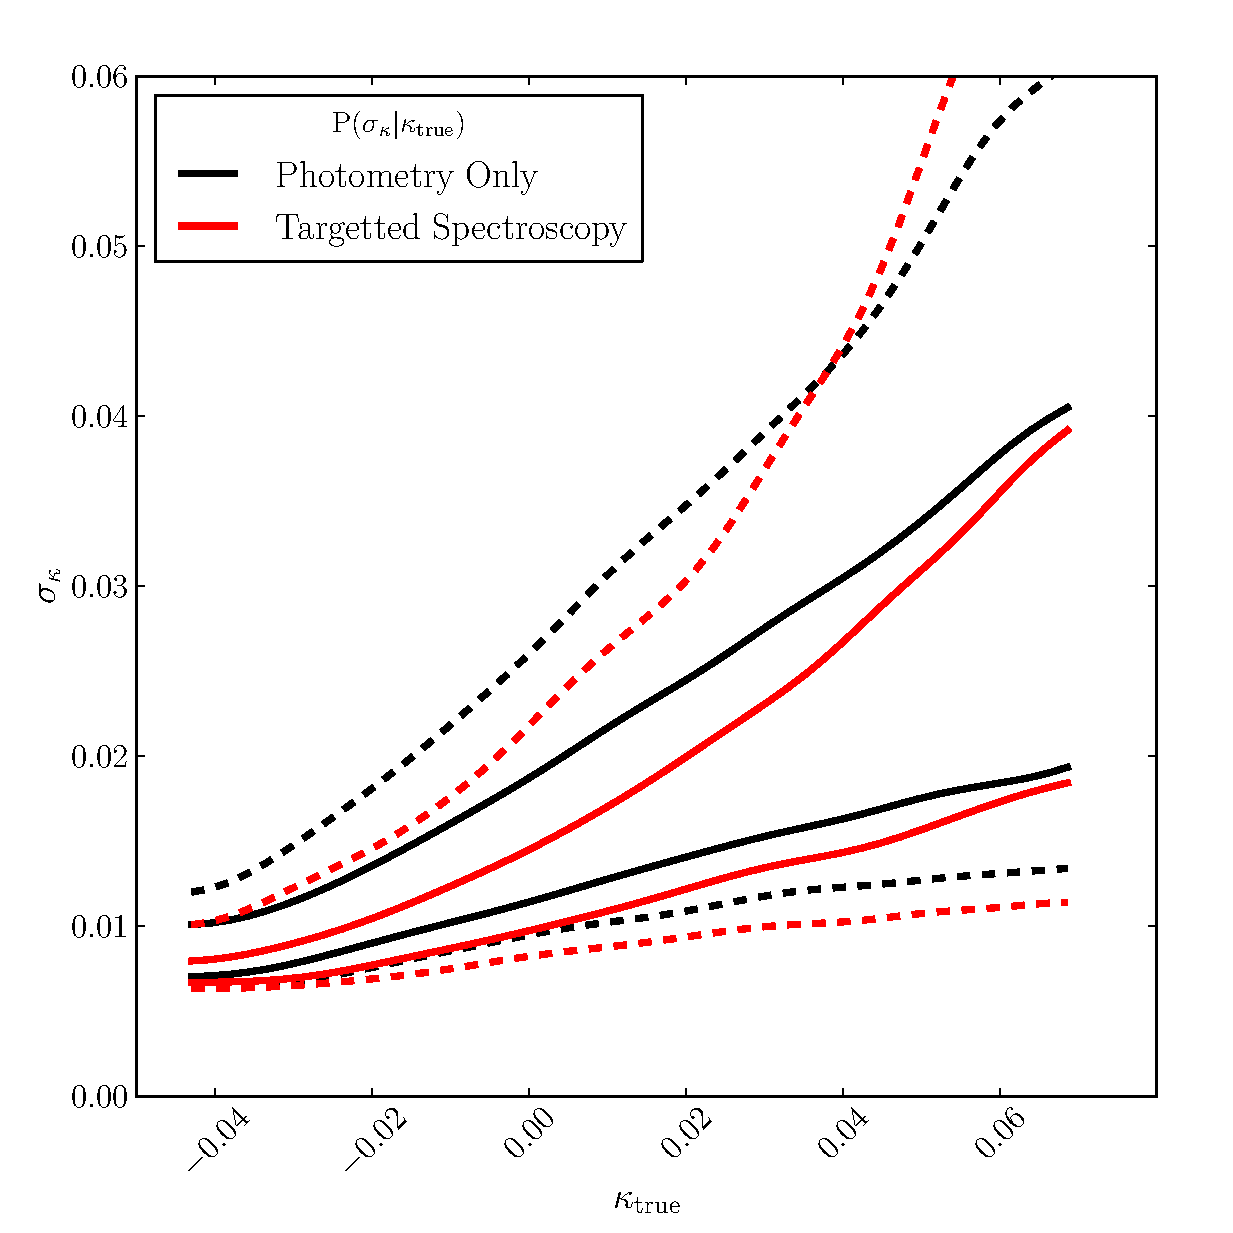
\includegraphics[width=\columnwidth]{figs/WidthvsHilbert.eps}
\caption{Width of the \infered PDF $\pr(\kappax|\data)$ as a function of 
the true convergence, $\kappaxtrue$, for two different data qualities. 
Black assumes only photometric redshifts for all objects,
while red assumes a campaign of targeted spectroscopy. The region between the
solid (dashed) lines contains 68\% (95\%) of lines-of-sight.}
\label{fig:widthsvsH}
\end{figure}
%%%%%%%%%%%%%%%%%%%%%%%%%

The best possible reconstructions of $\kappax$ will come from having a
spectroscopic redshift for every single object in each field.
\Fref{fig:reconwidths} shows the distribution of $\kappax$ posterior 
PDF widths for various data qualities: complete spectroscopic coverage results
in the smallest widths. In terms of telescope time, such a reconstruction
would likely be prohibitively expensive, but we investigate this scenario as
an ideal case. 

\comment{PJM: The following does not belong here because \Fref{fig:widthsvsH}
does not show results for spectroscopic redshifts only!}

Reconstructing the lines of sight with perfect knowledge of the
redshift but an uncertain stellar mass, we find that the width of
$\pr(\kappax|\data)$ grows with the expectation of $\kappax$ and the ray-traced $\kappatrue$
(\Fref{fig:widthsvsH}). The low $\kappax$ lines of sight are relatively empty,
and so there are few opportunities for uncertainties in the halo masses to
\propogate into $\kappax$ uncertainties; low $\kappax$ lines of sight can be reconstructed
more precisely than high $\kappax$ lines of sight.


% % % % % % % % % % % % % % % % % % % % % % % % % % % % % % % % % % % % % % % 

\subsection{Reconstructing $\kappax$ from photometry alone}

Inferring the stellar mass of a galaxy from its magnitude and colours requires
an estimate of how far away the galaxy is; without a spectroscopic redshift
the \infered stellar mass is less precise. However, obtaining photometry has
much lower observational cost; all upcoming large area photometric surveys
will reach 24th magnitude, providing sufficient data to reconstruct lines of
sight  {\it without} additional observations. In principle the photometric
redshift is correlated with the \infered stellar mass, however we do not model
this effect since the convergence from the outskirts of an individual halo is
only weakly \dependant on redshift at fixed mass due to the breadth of the
lensing kernel: the redshift uncertainty has only a small effect on the
inferred $\pr(\kappax|\data)$ in comparison to that of  the uncertain stellar
masses.  With only photometric redshifts, the uncertainty on $\kappah$ is
larger than in the spectroscopic case, and this \propogates into a broader
$\pr(\kappax|\data)$, as can be seen in \Fref{fig:reconwidths}. However, the
photometric reconstruction still typically produces a 50\% improvement
compared to the precision of the global $\pr(\kappax)$. 

\tom{With photometric data alone, $\kappah^{\rm med}$ can shift by $\sim$0.01
relative to $\kappah^{\rm med}$ given spectroscopic coverage. Since  the
$\kappax$ contribution of voids cannot change with data quality, the shift in
$\kappah^{\rm med}$ must be due to the asymmetric propagation of stellar mass
uncertainties into $\kappax$ uncertainties. As the stellar mass uncertainty
increases, $\kappah^{\rm med}$ is pushed higher.  To correctly calibrate 
$\pr(\kappax|\kappah^{\rm med},\data)$ one {\it must} include the data quality
used to generate $\kappah^{\rm med}$.}

We find that the width of $\pr(\kappax|\data)$ grows with the expectation
value of $\kappax$; this is shown in \Fref{fig:widthsvsH}. The low $\kappax$
lines of sight are relatively empty, and so there are few opportunities for
uncertainties in the halo masses to \propogate into $\kappax$ uncertainties.

%\flag{Is there a simple approximation for $\kappax$ and $\sigma_{\kappa}$ as a
%function of $\kappaxtrue$? This would be useful when making forecasts, writing
%proposals etc...}
%
%TEC: No. It's also not relevant to proposals since kappatrue isnt observable. One can ask is there
%a formula for sigmakappa given the expectation value of kappax. The answer to that is
%yes, but it depends on data quality. Concerning forecasting yes we would 
%want to use a simple approximation, but I don't think it has a place in this paper.
%When you/I/someone does the forecasting I'd like to be involved; I'll make the
%approximation then.


% % % % % % % % % % % % % % % % % % % % % % % % % % % % % % % % % % % % % % % 

\subsection{Reconstructing $\kappax$ with partial spectroscopic coverage}
\label{sec:obsMstar+z:targetedspec}

While a fully photometric reconstruction provides useful constraints on
$\pr(\kappax|\data)$, targeted spectroscopy can provide additional constraints
on the masses and redshifts of halos whose $\kappah$ contributions have the
largest absolute uncertainty. Obtaining spectra of bright ($i<22$) objects is
relatively fast with large telescopes: however, we find that if spectroscopic
redshifts were known for all $i<22$ galaxies in our fields the reconstruction
improves only slightly over the purely photometric reconstruction,  although
the improvement can depend strongly on the details of the particular line of
sight. Obtaining spectra for fainter objects would be correspondingly more
expensive, but if spectroscopic redshifts could be obtained for all $i<23$
galaxies (as part of a futuristic baryon acoustic oscillation survey, for
example) and all $i<24$ galaxies within 1 arcminute of the line of sight, then
we find that the $\pr(\kappax|\data)$ would be almost as precise as that from
having complete spectroscopic coverage (\Fref{fig:reconwidths}). If any object is
extremely close to the lines of sight our approximation of weakly lensing
mass-sheets will break down; also, neglecting baryonic effects will also be a poor
approximation; a spectrum will be needed
to adequately model systems with very well alligned pertrubers.
Consistent with our previous findings, the lowest $\kappax$ lines of
sight have the most constrained $\kappax$ PDFs.


%%%%%%%%%%%%%%%%%%%%%%%%%%%%%%%%%%%%%%%%%%%%%%%%%%%%%%%%%%%%%%%%%%%%%%%%%%%%%%

\section{Systematic Errors due to Sample Selection}
\label{sec:biases}


\begin{figure*}
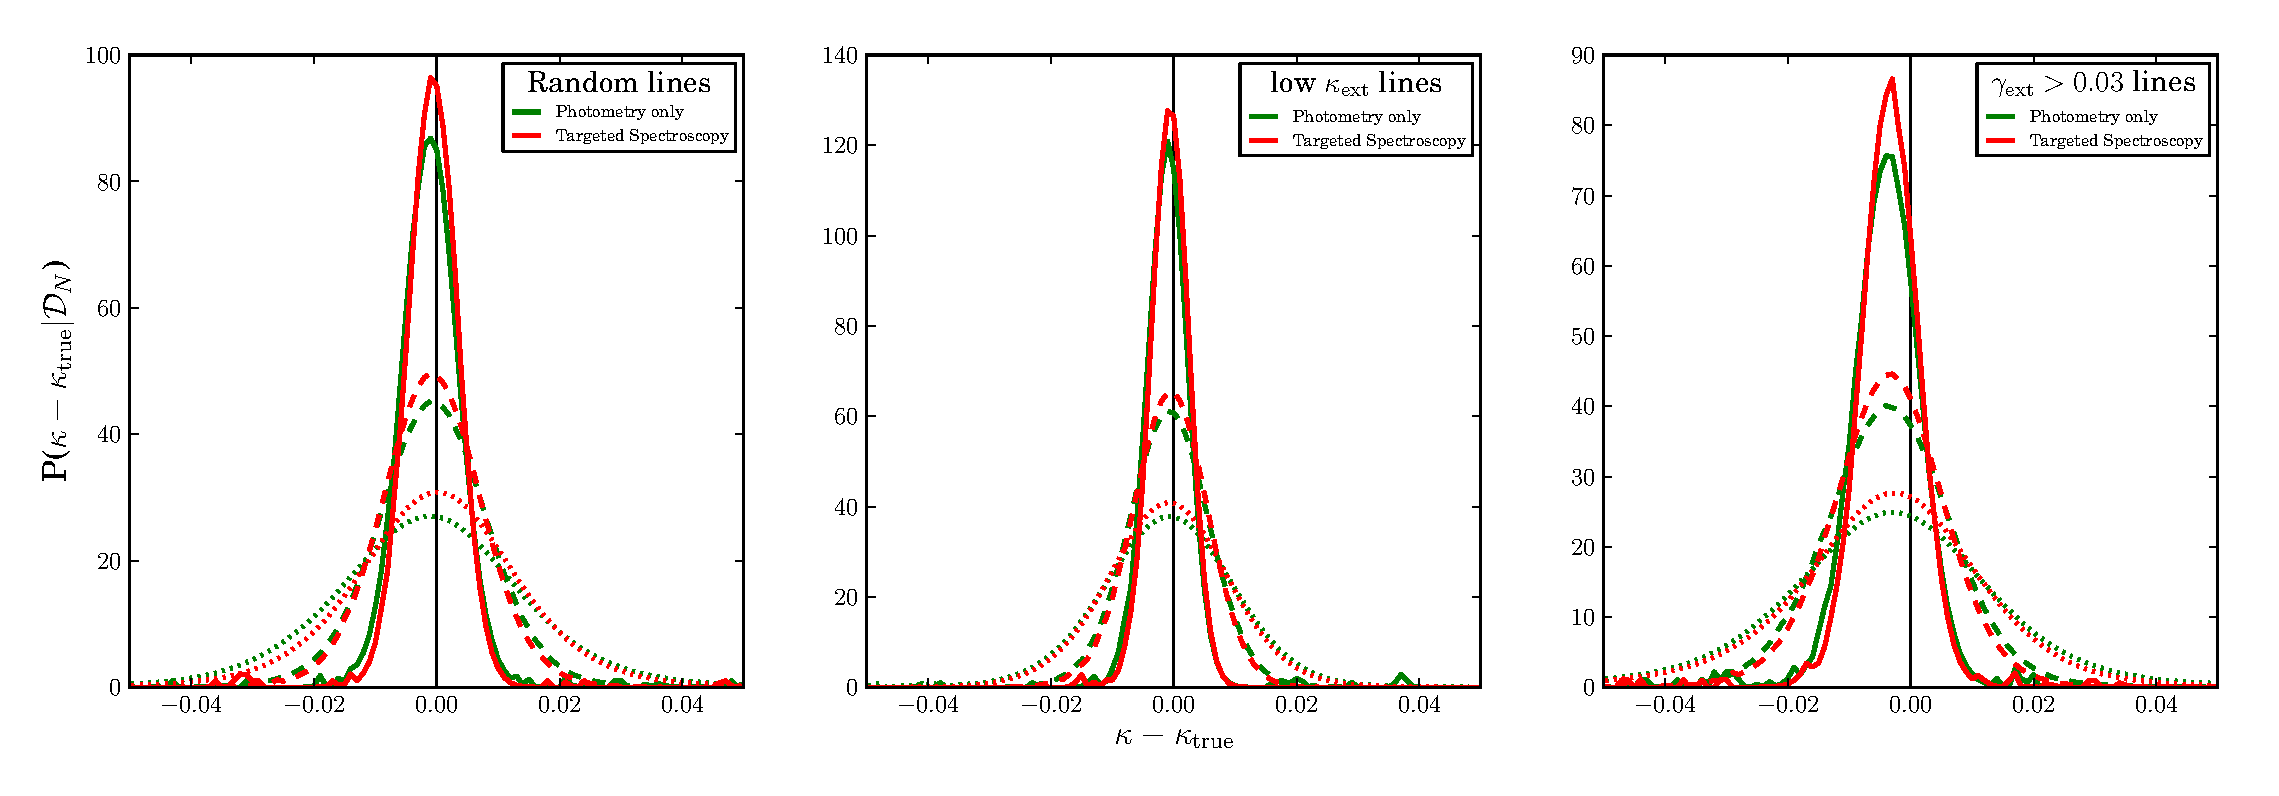
\includegraphics[width=\textwidth]{figs/biasplots.eps}
\caption{Accuracy in $\kappax$ from combining samples of lenses.  These plots
show the expectation value of $\prod_{i=1}^N \pr_i(\kappax-\kappaxtrue|\data)$ --
deviations from zero represent biases. The solid, dashed and dotted lines
correspond to combinations of  20, 5 and 2 sightlines respectively. Black
lines show the results \infered from photometry alone, whilst red lines show
the results  from the same targeted spectroscopy campaign described in 
\Sref{sec:obsMstar+z:targetedspec}. The three panels correspond to samples of
sightlines selected in different ways. Left: randomly selected lines of
sight.  Centre: sightlines randomly selected from the 33\% of lines whose
P($\kappax$) is most tightly constrained by our model.  Right: lines of sight
with external shear of 0.05 or greater.}
\label{fig:biasplots}
\end{figure*}

While it is good to reconstruct $\kappax$ precisely, it is more important that
$\kappax$ is reconstructed accurately. The reconstruction must not be biased. 
We quantify the accuracy of our reconstructed $\pr(\kappax|\data)$ in the
following way. By shifting the \infered $\pr(\kappax|\data)$ for each line of
sight by the true (ray-traced) convergence, we obtain a  PDF that should be
centred on zero; these offset PDFs can be multiplied together for multiple
lines of sight to emulate a joint likelihood analysis, and then test for
possible bias in it:
\be
\label{eq:bias}
\mathcal{P}_N = \prod_{i=1}^N \pr_i(\kappax-\kappax^{\rm true}|\data)
\ee
In this section, we quantify the bias as the size of the deviation in the
expectation value of $\mathcal{P}_N$ from zero. If the bias of $\mathcal{P}_N$
is smaller than the half-width of $\mathcal{P}_N$, our $\kappax$ inferences
can be considered accurate. Since the width of $\mathcal{P}_N$ decreases as
more sightlines are combined, a small bias will always 
eventually be found. In the context of measuring time-delay distance at the 
one percent level, the expectation value of $|\mathcal{P}_N|$ needs to be 
significantly less than 0.01. \tom{External convergence is not the only source
of uncertainty in measuring time-delay distance. Since the statistical
distance uncertainties due to lens modelling and time delay estimation are
likely to be at the 3-4\% level \citep{SuyuEtal2010}, convolving
$\mathcal{P}_N$ with a Gaussian of width $0.04/\sqrt{N}$ is a reasonable
approximation for the likely final uncertainty on time-delay distance.}


% \comment{From Sherry:
% Re: $P_N$:
% Not sure that this is the best way to quantify bias.  First of all, this
% doesn't include the modeling error of $\sim3-4\%$, so the number of lenses listed
% (for when <$P_N$> = half width of $P_N$) is underestimated.  Also, with this
% definition, a large number of lenses could be described as "biased" even if
% the resulting shift is say 0.0001, which won't really trouble us at all.  For
% example, what would the distributions look like in Fig.8 with 100 lenses? 
% Since the peaks of the red curves are within 0.01 of kappa_true, I would
% suspect that with a large number of lenses, the corresponding red curve would
% be within 0.01 of kappa_true.  The present day goal is to get H0 to 1\%, and
% it would be good to state somewhere that with targeted spectroscopy, one could
% recover kext at the 1\% level with a large sample of lenses.}

The source of systematic error that we investigate in this paper  is that of
sample selection: we define three different example selections of lines of
sight, and compute the bias  \phil{that would result (if left unaccounted
for)} in each one in turn, as a function of data quality. The results
described below are illustrated in \Fref{fig:biasplots}.


% % % % % % % % % % % % % % % % % % % % % % % % % % % % % % % % % % % % % % % 

\subsection{Selecting random lines of sight}
\label{sec:bias:random}

We first consider a purely random selection of lines of sight. With the purely
photometric reconstruction, there is no evidence of bias, even after combining
20 lines of sight. \tom{This result is a sanity check: if we had chosen lines
of sight with identical $\kappah^{\rm med}$ rather than $\kappah^{\rm
med}\pm0.003$, randomly selected lines of sight would have zero bias by
construction}. If lines of sight hosting time delay lenses are truely random, 
our method allows $\kappax$ to be reconstructed without inducing a bias (under
the basic assumptions that the universe is like the calibration simulation,
and the correct stellar-mass to halo-mass relation has been used). 


% % % % % % % % % % % % % % % % % % % % % % % % % % % % % % % % % % % % % % % 

\subsection{Selecting only the lines of sight with narrow $\pr(\kappax|\data)$}
\label{sec:bias:tightPDF}

Since follow-up campaigns (such as high resolution imaging, or time
variability monitoring) are expensive, it is likely that only a subset of
detected objects will be observed further. By pre-selecting objects that have 
the best-constrained convergence, the cosmological value per lens can be
increased. However, this selection \phil{(like any other)}
has the potential to induce a bias. It is
likely that only photometry will be available at the time of sub-sample
selection (although spectroscopic follow-up might be conducted at a later
date). We mimic such a selection by drawing lines of sight only from those in
the lowest third of $\sigma_{\kappa}$, given a purely photometric
reconstruction of their fields. 

We find that selecting the most tightly constrained lines of sight in this way
does not introduce a significant bias:  our reconstruction is most accurate
for the lowest $\kappax$ lines of sight. Combining 20 such systems, the bias
is at the 0.001 level.

Photometry of the field seems to be sufficient to adequately select these
empty lines of sight.  However, 
since lenses are typically massive galaxies and hence found in locally over-dense
environments, it is unlikely that  an almost empty line of sight would
actually  contain a lens; \phil{what we can say is that if the local
environment can be identified spectroscopically, and then the line
of sight mass distribution reconstructed using our method, selecting lenses
with low, well-constrained values of $\kappax$ will lead to an increase in
distance precision at no cost in bias.}

% % % % % % % % % % % % % % % % % % % % % % % % % % % % % % % % % % % % % % % 

\subsection{Selecting only high shear lines of sight}
\label{sec:bias:tightPDF}

Time delay lenses are often selected for follow-up based on their images'
brightness (to make monitoring observations less expensive), their images'
separation (to decrease the covariance between the ground-based image
light-curves), or the fact that they are quadruply-imaging rather than
doubly-imaging (since this yields 3 time delays instead of 1, a higher
magnification and a more informative Einstein Ring system). All three of these
properties favour lenses with high convergence and shear along their lines of
sight. Focusing on the quad selection, we might expect many of these systems
to have significant external shear (since the cross-section for 4 image
production is so sensitive to ellipticity in the lens mass distribution (or
equivalently, external shear due to the lens' environment). 

\phil{We can test the impact of such a shear selection by selecting only lines
of sight with an external shear above some threshold.  We define a somewhat
extreme selection  of $\gammax>0.05$, and find that in this sample, $\kappax$
would be systematically underestimated at the $\sim$0.008 level (corresponding
to a 0.8\% systematic error in distance).}  In the absence of other sources of
uncertainty, this systematic error would be significant in a sample of just 5
lenses; when including other time-delay distance uncertainties a 0.8\% bias would be
significant for $\sim$20 lenses. This systematic error is mitigated if only the lines of sight with both
$\gammax>0.05$ and well constrained $\pr(\kappax|\data)$ are used, but in this
case a bias at the $\sim$0.005 level remains. 

While $\gammax>0.05$ is likely to be a much stronger selection than would
occur in reality, it is  nevertheless worth noting from this example that the
reconstruction \proceedure \phil{can be biased if lens selection functions are
extreme and unaccounted for.} Since our model does not include shear
constraints it is not surprising that a selection function based on shear can
induce a bias. A more sophisticated model that includes the shear recovered
from the lens modelling might be less susceptible to this bias.

The halo model can also be used to estimate the external shear along a line of
sight: shear is an observable that can be extracted from strong lens
modelling. However, there is a degeneracy between internal and external shear.
When the Einstein Ring imaging data are very good it is possible to
disentangle external and internal shear \citep[\eg][]{SuyuEtal2010}, but there
are still significant uncertainties. \citet{WongEtal2011} attempted to match
the shear from strong lens models with a reconstruction of the local lens
group environment, but found a tension between the strong lens model and the
reconstruction of the environment. Given the \citet{WongEtal2011} results, it
is unclear whether the external shear from lens models can be reconciled with
a line-of-sight reconstruction. Alternatively, it may be possible  to infer
external shear using weak lensing information from near the line of sight.  If
the true external shear can be measured, it provides an additional constraint
on which of the \MS lines of sight are similar to the reconstructed line of
sight. \citet{SuyuEtal2012} found that in the case of 
RXJ1131-1231, combining shear constraints
with galaxy number count over-density gave a significantly different
$\pr(\kappax|\gamma,N_{45})$ compared to the PDF from number count
over-density alone, $\pr(\kappax|N_{45})$.

Extending our model to include shear we find that given
perfect knowledge of the halo mass and redshift the ray-traced external shear
$\gamma$ and the reconstructed external shear $\gamma_{\mathrm{h}}$  are
similar, with 68 percent of lines obeying
\be
\label{eq:shearineq}
|{\pmb{\gamma}_{\mathrm{ext}}-\pmb{\gamma}_{\mathrm{h}}}| < \mathrm{0.025}
\ee 
Future work should investigate whether $\gamma_{\mathrm{h}}$ can be used
to improve the accuracy and precision of $\kappax$ estimation, given a
reconstruction of the line of sight. 

%%%%%%%%%%%%%%%%%%%%%%%%%%%%%%%%%%%%%%%%%%%%%%%%%%%%%%%%%%%%%%%%%%%%%%%%%%%%%%

\section{Systematic Errors due to using an incorrect Stellar Mass--Halo Mass Relation}
\label{sec:SHAMfail}

\begin{figure*}
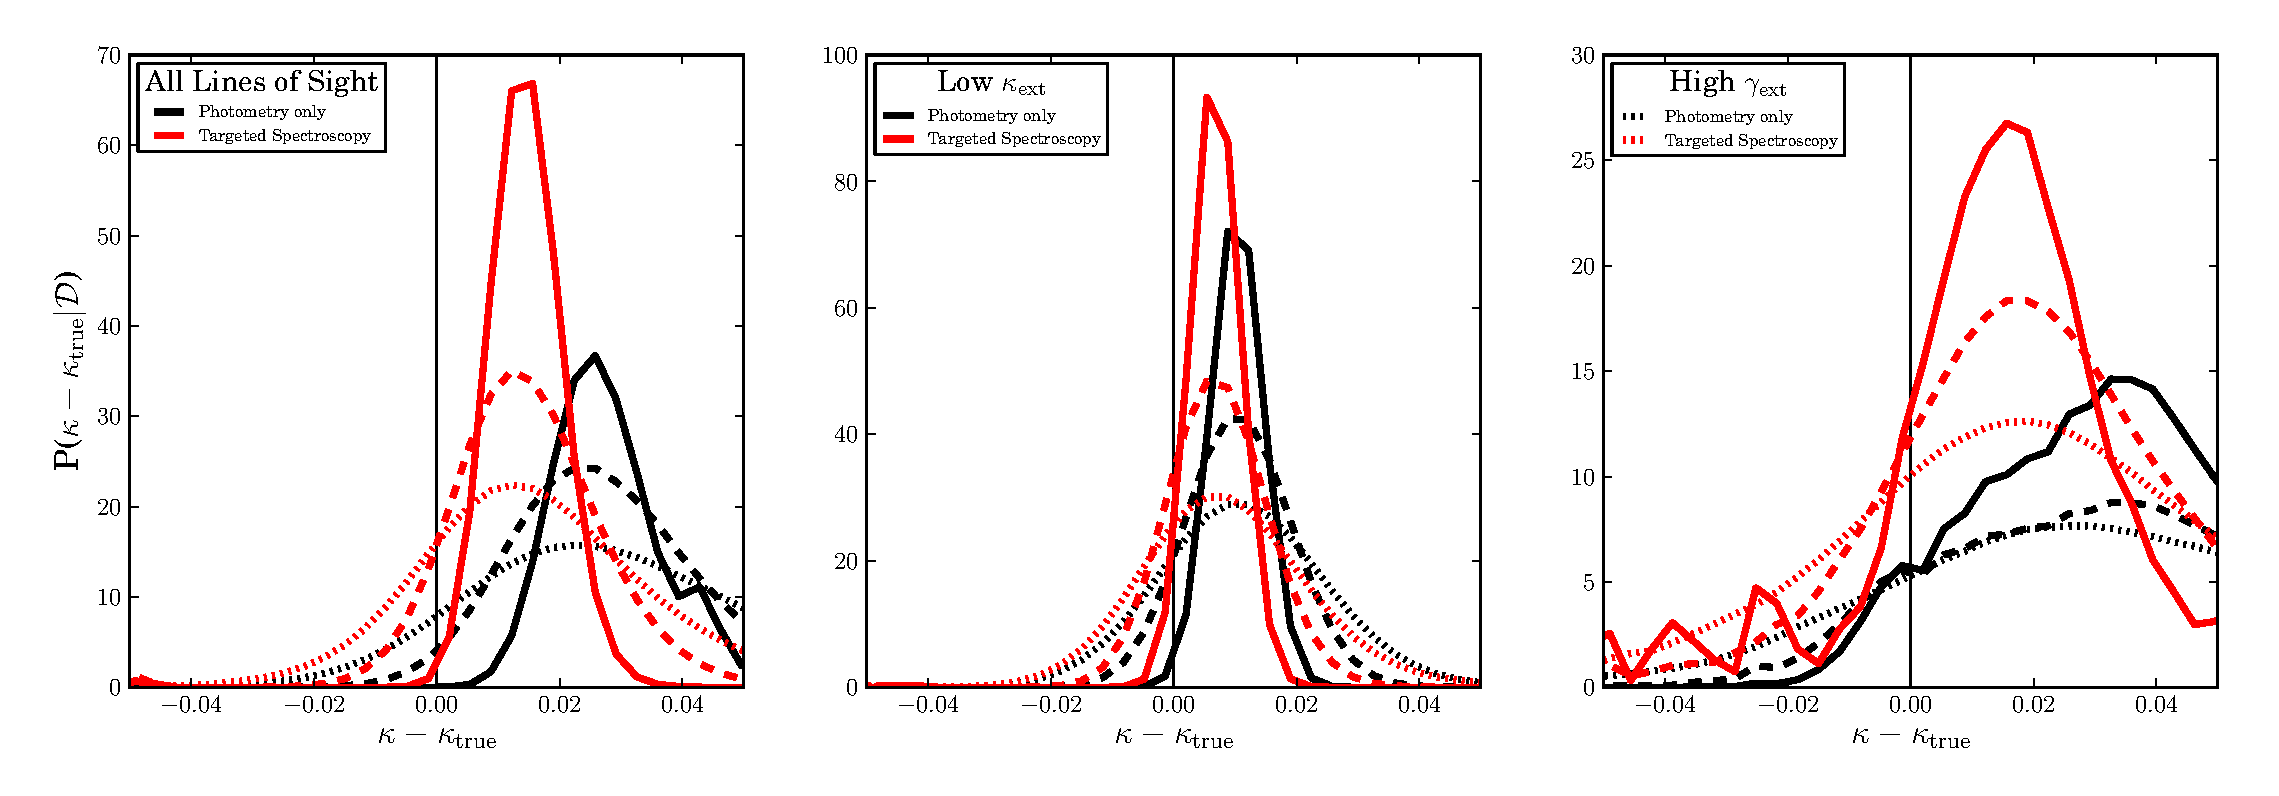
\includegraphics[width=\textwidth]{figs/SHAMbias.eps}
\caption{Systematic bias in $\kappax$ due to reconstructing lines of sight with the wrong stellar mass--halo mass relation. The real stellar masses were created using the relation of \citet{MosterEtal2010}, but the reconstruction and calibration assumes the relation of \citet{BehrooziEtal2010}.  These plots
show the expectation value of $\prod_{i=1}^N \pr_i(\kappax-\kappaxtrue|\data)$ --
deviations from zero represent biases. The solid, dashed and dotted lines
correspond to combinations of  20, 5 and 2 sightlines respectively. Black
lines show the results \infered from photometry alone, whilst red lines show
the results  from the same targeted spectroscopy campaign described in 
\Sref{sec:obsMstar+z:targetedspec}. The three panels correspond to samples of
sightlines selected in different ways. Left: randomly selected lines of
sight.  Centre: sightlines randomly selected from the 33\% of lines whose
P($\kappax$) is most tightly constrained by our model.  Right: lines of sight
with external shear of 0.05 or greater.}
\label{fig:SHAMbias}
\end{figure*}

\new{
Throughout this work we have assumed that the universe's halos are populated with galaxies whose stellar masses are determined purely by the \citet{BehrooziEtal2010} Stellar Mass--Halo Mass relation. The real universe is unlikely to follow this relation perfectly; the result is that an ensemble of real lines of sight will differ from the ensemble of calibration lines of sight, potentially introducing a systematic error to the reconstructed convergence.

It is hard to test the size of this sytematic error, since we do not know how much the real universe differs from the chosen Stellar Mass--Halo Mass relation. As wider and deeper surveys are conducted more data will become available with which to construct the Stellar Mass--Halo Mass relation; this should drive the infered Stellar Mass--Halo Mass relation closer to the truth. We are only interested in testing the effect of changing the Stellar Mass--Halo Mass relation in a way that is consistant with observational constraints; improving the observational contraints on the Stellar Mass--Halo Mass relation will decrease the the size of the systematic error on reconstructed $\kappax$ induced by assuming a specfic Stellar Mass--Halo Mass relation.

To estimate the potential size of this systematic error we use the Behroozi relation to generate the stellar masses of our calibration lines of sight, but the stellar mass--halo mass relation of Moster for the ``real'' lines of sight that are reconstructed. For halos masses of $\sim 10^{12} \Msun$ both stellar mass--halo mass relations estimate a stellar mass of $\sim 10^{10.5} \Msun$, but for halos more massive that this the stellar masses generated from the Moster relation are systematically higher than those generated from the Behroozi relation. At halo masses of $\sim 10^{14} \Msun$ the best fit stellar masses differ by $\sim 0.25$ dex. 

Applying our Behroozi--based reconstruction to lines of sight with Moster stellar masses results in systematically overestimating $\kappax$. In \Fref{fig:SHAMbias} we show the resulting bias on the inferred $\kappax$ after combining several lines of sight. With a purely photometric reconstruction there is a typical systematic bias of $\sim 0.025$ on the reconstructed convergence, although it can be shrunk to $\sim 0.01$ if only the low $\kappax$ lines of sight are used, however for the high shear lines of sight the bias is $\sim 0.04$. It is not suprising that the low $\kappax$ lines of sight are least affected by changes in the stellar mass--halo mass relation. Low $\kappax$ lines of sight are relatively empty hence their $\kappah$ values are small and do not change significantly with stellar mass--halo mass relation. The high shear lines of sight have significantly overestimated $\kappax$ since they tend to lie close to massive halos. This is the regime where the Moster and Behroozi relations are most different. Interestingly overestimating the $\kappah$ values of high shear lines of sight pushes them into the region where the $\kappah$ to $\kappax$ calibration is least certain; this has significantly decreased the precision of the reconstructed $\kappax$. 

Despite the systematic errors the photometric reconstruction is still sufficient to choose the best lines of sight for spectroscopic follow-up. With targetted spectroscopy the systematic error decreases to $\sim 0.014$ for the ensemble, $\sim 0.005$ for the low kappa sample and $\sim 0.018$ for the high shear sample. This result provides further motivation for prioritizing the lenses that reside on the underdense lines of sight.

The systematic errors reported herein may be overly pessimistic; the bias is due to differences in the stellar masses predicted for high mass halos. If observations can discriminate between the high mass end of the Behroozi and Moster relations then the systematic error on the reconstruction will decrease.
}

%%%%%%%%%%%%%%%%%%%%%%%%%%%%%%%%%%%%%%%%%%%%%%%%%%%%%%%%%%%%%%%%%%%%%%%%%
%\section{Improving precision by including additional information}
%\notes{placeholder for shear}
%%%%%%%%%%%%%%%%%%%%%%%%%%%%%%%%%%%%%%%%%%%%%%%%%%%%%%%%%%%%%%%%%%%%%%%%%

\section{Discussion}
\label{sec:discuss}

% \comments{
% We have shown that reconstructing the matter due to halos along any line of
% sight can improve the constraints on the external convergence along that line
% of sight, with, depending on sample selection,  the width of
% $\pr(\kappax|\data)$ being up to a factor of two smaller than the global
% $\pr(\kappax)$, and  we have quantified the residual bias in the $\kappax$
% estimates under our calibration assumptions. We now revisit these assumptions.
% }

The total convergence along a line of sight is strongly correlated with the
reconstructed $\kappah$. However, since our model ignores voids and assumes
all halos follow a spherical truncated-NFW profile our halo model does not
include all of the relevant physics; hence, the width of our resulting
$\pr(\kappax|\data)$ is still typically $\sim$0.01 for any given lightcone,
even assuming perfect knowledge of every halo's virial mass and redshift. To
make further progress a more advanced treatment of both voids and halos will
be needed. \citet{KarpenkaEtal2012} find that their supernova data prefer, in
the context of their simple halo model, a truncated isothermal profile for the
galaxy mass distributions. Galaxy-galaxy and cluster-galaxy  lensing studies
\citep[\eg][]{GavazziEtal2007,JohnstonEtal2007, LagattutaEtal2010} also suggest an approximately
isothermal profile for the mass-shear correlation function; however, at large
radii these profiles are dominated by the effects of neighbouring halos, which
are already taken into account by our model.  Further iterations on the
analysis presented here should include the stellar mass distributions that
cause the isothermal density profiles in the centres of galaxies, although we
do not expect this to have a big impact on the reconstructions. Likewise, 
halo ellipticity
may have some small effect on the predicted convergence. It
is possible that baryonic physics may alter the radial profile of dark
matter halos, even on large scales. \citet{Semboloni+2012} found that baryonic
physics had a 30-40\% impact on three-point shear statistics, it is unclear
how baryons affect one-point convergence statistics compared to the pure dark
matter simulations used in this work.

Clusters, filaments and voids are more difficult to model, but simple forms
could in principle be derived from the structures found in the simulations,
and included in the halo model in some way.  Most importantly for the highest
$\kappax$ lines of sight will be a better group and cluster model:
\citet{MomchevaEtal2006} and  \citet{WongEtal2011} recommend using models
where dark mass is assigned to both galaxy-scale halos and halos for the
groups and clusters they occupy. To make this work, one could incorporate a
group and cluster finder, and then infer halo mass from optical richness
\citep[\eg][]{MaxBCG} in tandem with BCG stellar mass. \new{A group finder would also
allow us to identify central and satellites galaxies; in this work we have neglected
the differences between central halos and satellites. However, given perfect knowledge of halo masses
we found that only in 5 percent of sightlines do satellites
contribute over 20 percent of the sightline's total $\kappax$. Introducing a group finder
is unlikely to provide major improvement to the reconstruction of satellites.}
\tom{Meanwhile,
improving the modelling of voids could be done using suggestions by
\citet{voids2} or \citet{voids1} combined with a void finder such as in
\citet{voids3}. Combining an advanced halo model with a void model will allow
a direct test of the halo approximation: using real photometric data one could
reconstruct lines of sight and compare against measured weak lensing shears.
This would ensure that the reconstruction model reproduces the contents of the
real universe, rather than a particular simulation.}

% \comments{Interestingly, we have found that it is the most empty lines of sight that 
% can be reconstructed with the highest precision. $\kappax$ estimates for empty
% lines of sight receive few contributions from halos, and a large contribution
% from voids; since they have the tightest PDFs after the reconstruction it
% seems that our model's biggest uncertainties are driven by naively
% reconstructing halos rather than neglecting voids. With a photometric
% reconstruction of the field there is a significant broadening, but the
% resulting precision is still typically 50\%  higher than using the global
% $\kappax$ distribution.
% 
% Since the uncertainty on $\pr(\kappax|\data)$ is $\sim$0.01 even
% with perfect knowledge of halo mass and redshift, it seems that modelling uncertainties
% from voids, deviations from sphericity and dark matter clumping within the
% main halo dominate the total $\kappax$ uncertainty even with very
% uncertain stellar masses. Inferring halo ellipticity and dark matter
% clumping will likely always remain a difficulty for line of sight
% reconstruction; but as \Fref{fig:magcut} shows, observing deeper
% than 24th magnitude does not significantly help the reconstruction.
% }

% \comments{For a small fraction of lines of sight, $\pr(\kappax|\data)$ remains very
% broad even after applying our reconstruction; these lines of sight are
% typically the most over-dense lines of sight in the universe. For
% time-delay cosmography the most observationally expensive tasks are the
% light-curve monitoring and high resolution follow-up imaging and spectroscopy,
% while making photometric observations of a
% 4$\times$4 arcminute patch of sky survey down to 24th magnitude is
% relatively cheap. We have shown that with a single epoch observation of
% the region around a strong lens it is possible to infer $\pr(\kappax|\data)$.
% If a line of sight has a broad $\pr(\kappax|\data)$ it can be rejected {\it
% before} the investment of follow-up. We find that
% selecting only the lines of sight with the most tightly constrained
% $\pr(\kappax)$ does not induce a bias in $\kappax$, and hence distance.
% For the most over-dense lines of sight,
% the precision of $\pr(\kappax|\data)$ is improved noticeably by the addition
% of spectroscopic information; currently insufficient time-delay systems are
% know to choose a subset based on their reconstructed $\pr(\kappax|\data)$.
% Spectroscopic coverage will definitely be useful for extracting cosmology from
% over-dense lines of sight.
% }
% %%%%%%%%%%%%%%%%%%%%%%%%%%%%%%
% \comments{%
% \begin{figure}
% 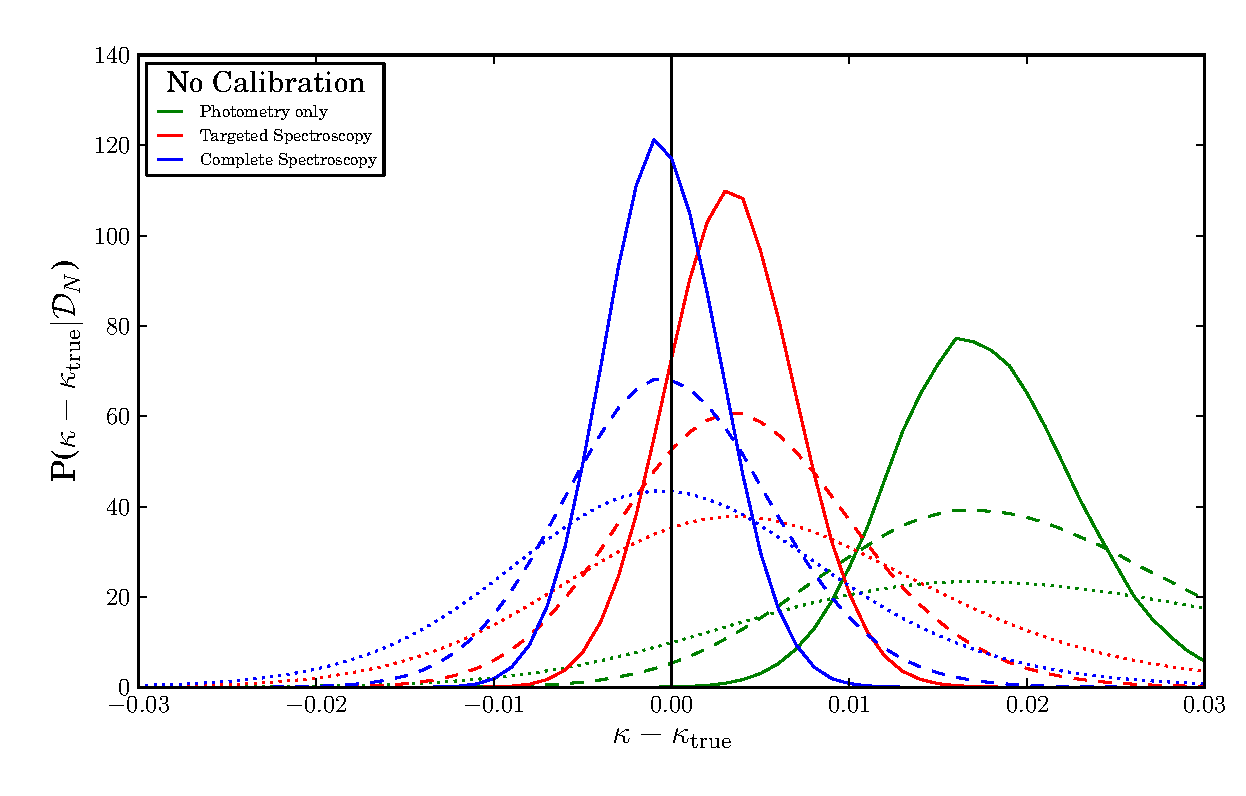
\includegraphics[width=\columnwidth]{figs/biasplots3.eps}
% \caption{Convergence estimation accuracy using the full  $\pr(\kappax|\kappah)$
% distribution, rather than its median.  As in \Fref{fig:biasplots}, solid,
% dashed and dotted lines show combinations of 20, 5 and 2 lines of sight
% respectively, while green lines show the inferences 
% from photometry alone, red lines from photometry and targeted spectroscopy 
% (assuming a spectroscopic redshift for all
% halos with $i<23$ and all halos within 1 arcminute and $i<24$), and blue lines
% from the unrealistic assumption of a spectroscopic redshift for all galaxies
% in the field. }
% \label{fig:no-median-tricks}
% \end{figure}
% }%
%%%%%%%%%%%%%%%%%%%%%%%%%%%%%%

The reduction of $\pr(\kappah|\data)$ to just its median value, before using
it to look up the appropriate $\pr(\kappax)$ from the simulated sightline
ensemble, is reminiscent of the procedure followed by \citet{SuyuEtal2010},
and Greene et al (submitted). The reconstruction method presented here can be
seen as the limiting case of the weightings explored by Greene et al: rather
than using weighted number counts in an aperture, we treat each galaxy
individually, and predict $\kappa_{\rm h,obs}^{\rm med}$ for use in their
place. Given photometry alone, our reconstruction represents a $\sim$50\% improvement of
the precision compared the number counts used in \citet{SuyuEtal2010}. Greene et al.
made important progress for the most over-dense lines of sight; our
reconstructions are $\sim$30\% more precise than those of Greene et al.
The use of relative overdensities by Suyu et al. and Greene et al. may decrease 
their sensitivity to the choice of calibration simulation; this work's use of
absolute convergence may be less robust to changes in the calibration simulation. 


% \comments{ One
% significant disadvantage of these types of method is that they impose a
% bottleneck in the flow of information. Once you have compressed to one number,
% it is difficult to incorporate more information later; you have to recompute
% all the calibrations. Using the full PDF for $\kappah$ is the more correct
% thing to do: at present, however, it suffers from significant bias in the
% photometric data case. \Fref{fig:no-median-tricks} shows how $\kappax$ is
% overestimated, as a result of the high scatter in halo mass for objects with 
% high stellar mass. As has already been noted, 
% future work should focus on increasing the precision of the halo
% mass estimates. 
% }

In this work, we have used  the \MS as a calibration tool. If the real
Universe is not like the \MS, then this calibration will be incorrect.
Repeating this study using a different simulation to make the test catalogues
would allow us to quantify the sensitivity of our results to the simulation
used. Similarly the use of a different semi-analytic model to paint galaxies
onto halos would enable similar exploration of these systematic errors. 
\citet{SuyuEtal2010}
used the relative over-density to mitigate the effect of simulatioan and
simulation, but it does not completely remove the dependence on simulation.
\new{We have tested the effect of using a different stellar mass--halo mass relation
and found that this can induce significant systematic biases if the true relation is unknown.} Future work should include
investigating the robustness of the reconstruction to these systematic errors \new{and develope proscriptions that mitigate against them}

% \comments{In particular, the method presented here is tied to the simulations at two
% points: the prior PDF for $\kappah$, and the conditional distribution
% $\pr(\kappax|\kappah)$ used to convert halo model convergence to total
% convergence. The first tie could potentially be avoided if the halo mass
% estimation gave rise to a reasonable $\pr(\kappah|\data)$ on its own.
% Possibilities for improving the precision of the halo mass estimation are
% discussed above. The second tie is more difficult, since breaking it means
% modelling the unseen mass structures and voids. It
% should be possible to infer hierarchically  the parameters of a flexible model
% for these things from the data itself, as demonstrated by
% \citet{KarpenkaEtal2012} (albeit under the assumption of scatter-free scaling
% relations) -- how this affects the cosmographic precision is to be
% investigated. When working with wide field imaging surveys,  weak lensing shears will be
% available around every line of sight:  fitting these with the halo models
% described here in order to constrain the hyper-parameters of the model presents a 
% possible test of our halo model prescription against real observations.
% }
%%%%%%%%%%%%%%%%%%%%%%%%%%%%%%%%%%%%%%%%%%%%%%%%%%%%%%%%%%%%%%%%%%%%%%%%%

\section{Conclusions}
\label{sec:conclude}

In this work we have investigated a simple halo model prescription for
reconstructing all the mass along a line of sight to an intermediate redshift
source. We have used the ray-traced lensing convergence along lines of sight
through the Millennium Simulation to calibrate estimates of the total
convergence made by summing the convergences due to each object in a
photometric catalogue. Having found that the reconstruction process is
accurate given this calibration and perfect knowledge of halo mass and
redshift, we investigated the effects of reasonable uncertainties in the
stellar mass and redshift of each halo, and propagated these uncertainties
into a $\pr(\kappax|\data)$ for each line of sight. We also defined three
different possible line of sight selections, and investigated the possible 
bias induced by these selections. We draw the following conclusions:

\begin{itemize} 

\item Despite our model's simplicity, its reconstructed $\kappah$ values are
good tracers of $\kappax$. $\kappah$ is biased due to our ignorance of voids,
groups and clusters, and the unseen mass in small halos and filaments, but we
find that this can be calibrated out using the Millenium Simulation
catalogues. We found that with perfect knowledge of every halo's mass and
redshift,  calibrated reconstruction of a typical line of sight  gives an
unbiased estimate of $\kappax$ that is not perfect, but is $1.8$ 
times more precise than the global
$\pr(\kappax)$. This factor quantifies the limit to which the halo model can
represent the external convergence due to line of sight mass structure.

\item With uncertain halo masses and redshifts, we find that
$\pr(\kappah|\data)$ can still be calibrated in order to infer
$\pr(\kappax|\data)$ from the ensemble of simulated lines of sight, but the
resulting PDFs tend to be much broader than for perfect halo mass and redshift
reconstructions.

\item It is very rare for halos further than 2 arcminutes from the line of
sight to make a significant contribution to $\pr(\kappax|\data)$; likewise, 
including
halos whose host galaxy is less luminous than $i=24$ does not significantly
improve our reconstructions.  A photometric survey to this depth of a
4$\times$4 arcminute patch around the target would approach the limiting
uncertainties of our simple reconstruction recipe, and yield a 
$\pr(\kappax|\data)$ that has, on average, a width of 0.016 (inducing a $\sim$1.6\%
uncertainty on time-delay distances). This is 1.5 times
less broad than the global $\pr(\kappax)$. 

\item  For the most over-dense lines of sight, the reconstruction produces a
broad PDF; conversely, we find that the lines of sight with the sharpest
inferred $\pr(\kappax|\data)$ are typically under-dense. Since the
reconstructions described here can be performed before follow-up time is
invested, it will be possible to select targets by the precision of their
$\kappax$ estimates. This will be useful in an era when there are more known
lenses than can be followed-up. Photometric data are sufficient to select the best lines of sight for
follow-up. Spectroscopic coverage helps to tighten  $\pr(\kappax|\data)$ for
most lines of sight.
% , but is of less use for low $\kappax$ lines of
% sight.

\item Selecting from the highest precision 33\% of the reconstructed lines of
sight results in a sample with low bias, $\sim$0.1\% in terms of the
time-delay distance. \tom{For these lines of sight the reconstructed
$\pr(\kappax|\data)$ induces a statistical uncertainty of $\sim$1\% on
individual time-delay distances.}

\item Conversely, selecting lines of sight with high shear ($|\gamma| > 0.05$; 
a somewhat extreme selection, but one that  could potentially arise from 
focusing on four-image or wide separation lenses) results in a sample with
bias of 0.8\% in time delay distance (and hence $H_0$). Including realistic estimates of other
sources of uncertainty a systematic error of 0.8\% would become significant in
a sample of $\sim$20 lenses. The addition of shear constraints to our model might
alleviate this potential systematic.

\item \new{Reconstructing a line of sight with an incorrect stellar mass--halo mass relation can introduce systematic errors on the inferrred time-delay distance at the percent level. This error can only be reduced by tightening the observational limits on the stellar mass--halo mass relation at the high mass end.}

% \item With only a photometric reconstruction of all time delay lens fields,
% and following up only the systems with the most precise $\kappax$ estimates,
% the width of the dominant statistical uncertainty in time-delay cosmography
% can be halved, without inducing biases at the one percent level.

\end{itemize}

% PJM: Im not sure this is the right note to end on. 

% TEC: I liked it! but it's open to discussion.


% External convergence is not the only uncertainty in time delay cosmology, but
% for systems like B1608$+$656 it is the dominant one. For most lines of sight
% lens modelling induces uncertainties at the $\sim$4 percent
% level, which far exceeds the typical $\kappax$ uncertainties after applying our
% reconstruction \proceedure. By using reconstruction methods such as that
% explored here to select the most appropriate 
% lenses for follow-up, the uncertainties due to line of sight
% convergence will become a sub-dominant source of error.

While we have tested our reconstruction method against realistic simulations
of line of sight mass distributions in the Universe, our method is also 
calibrated to these simulations. Testing this assumption in the short term,
and replacing it with an empirical calibration (or hierarchical inference) in
the longer term, are worthy goals for future work. The halo model framework is
flexible enough to enable many such improvements, including, quite naturally,
the incorporation of more information from observations. 


%%%%%%%%%%%%%%%%%%%%%%%%%%%%%%%%%%%%%%%%%%%%%%%%%%%%%%%%%%%%%%%%%%%%%%%%
%%  ACKNOWLEDGMENTS
%%%%%%%%%%%%%%%%%%%%%%%%%%%%%%%%%%%%%%%%%%%%%%%%%%%%%%%%%%%%%%%%%%%%%%%%

\section*{Acknowledgements}
 
TEC thanks Vasily Belokurov for supervision, guidance and suggestions.
We thank Risa Wechsler and Peter Behroozi 
for useful discussions and suggestions. We are grateful to the referee
for suggesting improvements to the original manuscript.
TEC acknowledges support from STFC in the form of a research studentship.
%
PJM was given support by the Kavli Foundation and the Royal 
Society, in the form of research fellowships.
%
MWA \ldots
%
SH \ldots
%
SHS \ldots
%
TT acknowledges support from the NSF through CAREER award NSF-0642621,
and from the Packard Foundation through a Packard Research Fellowship.
% 
LVEK acknowledges the support by an NWO-VIDI programme subsidy
(programme number 639.042.505).
%
This research is supported in part by the National Science Foundation under
Grant No. PHY99-07949.



%%%%%%%%%%%%%%%%%%%%%%%%%%%%%%%%%%%%%%%%%%%%%%%%%%%%%%%%%%%%%%%%%%%%%%%%%%%%%%
%  APPENDICES
%%%%%%%%%%%%%%%%%%%%%%%%%%%%%%%%%%%%%%%%%%%%%%%%%%%%%%%%%%%%%%%%%%%%%%%%%%%%%%

\appendix

%%%%%%%%%%%%%%%%%%%%%%%%%%%%%%%%%%%%%%%%%%%%%%%%%%%%%%%%%%%%%%%%%%%%%%%%%%%%%%

\section{Inferring $\Mhalo$ given a noisy measurement of $\Mstarobs$}
\label{appendix:MSMH}

To estimate the convergence caused by a halo we need to know its mass; how can 
halo mass be \infered from a noisy estimate of the stellar mass $\Mstarobs$
of a galaxy at redshift $z$. We seek the posterior
PDF $\Pr(\Mhalo|\Mstarobs,z)$, which can be expanded as follows:

\begin{eqnarray}
&& \Pr(\Mhalo|\Mstarobs,z) = \notag\\
&& \int d\Mstar \Pr(\Mhalo|\Mstar,z) \Pr(\Mstar|\Mstarobs,z), \notag\\
&\propto& \int d\Mstar \Pr(\Mstarobs|\Mstar) \Pr(\Mstar|\Mhalo,z) \Pr(\Mhalo|z),
\label{eq:mhalo-mstar}
\end{eqnarray}
where we have used Bayes' Theorem twice to replace
$\Pr(\Mhalo|\Mstar,z) \Pr(\Mstar|z)$ with 
$\Pr(\Mstar|\Mhalo,z) \Pr(\Mhalo|z)$, and 
to invert $\Pr(\Mstar|\Mstarobs)$ into the sampling
distribution $\Pr(\Mstar|\Mstarobs)$, which we recognise as the likelihood
function for the observed stellar mass. Note that the ``true'' $\Mstar$ of the
galaxy is marginalised out: we are only interested in inferring the halo
mass. The last two terms in
\eqref{eq:mhalo-mstar} are the $\Mstar-\Mhalo$ relation from
\citet{BehrooziEtal2010}, and the halo mass function $\Pr(\Mhalo|z)$, at the
given redshift. We can
tabulate the product of these two from our Millennium Simulation catalogue,
constructing a two-dimensional histogram of halo masses and their associated
true stellar masses (drawn from the Behroozi relation). 

For each galaxy, we compute the likelihood function for its $\Mstarobs$ as a
function of the unknown $\Mstar$, and multiply it by our tabulated joint PDF.
This heavily downweights halos with $\Mstar$ values outside the observed
range. We then do the marginalisation integral by Monte Carlo, drawing
(two-dimensional) sample parameter vectors
from the down weighted histogram, discarding the $\Mstar$ values, and
constructing a one-dimensional histogram that is an estimate of
$\Pr(\Mhalo|\Mstarobs)$.

If the redshift of the galaxy is uncertain, we need to take this
uncertainty into account; for example, for each sample drawn from the
photometric redshift posterior PDF $\Pr(z|{\rm colors})$, we can draw a
sample $\Mhalo$ using the above procedure.

%%%%%%%%%%%%%%%%%%%%%%%%%%%%%%%%%%%%%%%%%%%%%%%%%%%%%%%%%%%%%%%%%%%%%%%%%%%%%%
%  REFERENCES
%%%%%%%%%%%%%%%%%%%%%%%%%%%%%%%%%%%%%%%%%%%%%%%%%%%%%%%%%%%%%%%%%%%%%%%%%%%%%%

% MNRAS does not use bibtex, input .bbl file instead. 
% Generate this in the makefile using bubble script in scriptutils:

% bubble -f paper-lcr.tex references.bib 
% %%%%%%%%%%%%%%%%%%%%%%%%%%%%%%%%%%%%%%%%%%%%%%%%%%%%%%%%%%%%%%%%%%%%%%%%
%
% Pangloss: Testing the reconstruction method
%
%%%%%%%%%%%%%%%%%%%%%%%%%%%%%%%%%%%%%%%%%%%%%%%%%%%%%%%%%%%%%%%%%%%%%%%%

\documentclass[useAMS,usenatbib,a4paper]{mn2e}
%% letterpaper
%% a4paper

%\voffset=-0.6in

% Packages:
\input psfig.sty
\usepackage{xspace}
\usepackage{graphicx}
\usepackage{amssymb}
\usepackage{amsmath}

% Macros:
\input{macros.tex}
\input{addresses.tex}

%%%%%%%%%%%%%%%%%%%%%%%%%%%%%%%%%%%%%%%%%%%%%%%%%%%%%%%%%%%%%%%%%%%%%%%%

\title[Line of Sight Mass Reconstruction]
{Reconstructing the Lensing Mass in the Universe \\
from Photometric Catalogue Data}
    
\author[Collett \etal]{%
  Thomas~E.~Collett$^{1}$\thanks{\collettemail},
  Philip~J.~Marshall$^{2}$,
  Matthew~W.~Auger$^{1}$,
  Stefan~Hilbert$^{3}$,
\newauthor{%
  Sherry~H.~Suyu$^{4,3,5}$,
  Zachary~Greene$^{4}$,
  Tommaso~Treu$^{4}$\thanks{\packard},
  Christopher~D.~Fassnacht$^{6}$,}
\newauthor{%
  L\'eon~V.~E.~Koopmans$^{7}$,
  Maru\v{s}a Brada\v{c}$^{6}$,
  Roger~D.~Blandford$^{3}$} 
  \medskip\\
  $^1$\ioa\\
  $^2$\oxford\\
  $^3$\kipac\\
  $^4$\ucsb\\
  $^5$\asiaa\\
  $^6$\davis\\
  $^7$\kapteyn
}

%%%%%%%%%%%%%%%%%%%%%%%%%%%%%%%%%%%%%%%%%%%%%%%%%%%%%%%%%%%%%%%%%%%%%%%%

\begin{document}
             
\date{to be submitted to MNRAS}
\pagerange{\pageref{firstpage}--\pageref{lastpage}}\pubyear{2012}

\maketitle           

\label{firstpage}

%%%%%%%%%%%%%%%%%%%%%%%%%%%%%%%%%%%%%%%%%%%%%%%%%%%%%%%%%%%%%%%%%%%%%%%%

\begin{abstract} 

High precision cosmological distance measurements towards individual objects
such as time delay gravitational lenses or type Ia supernovae are affected by
weak lensing perturbations by galaxies and groups along the line of sight. In
time delay gravitational lenses, ``external convergence,'' $\kappax$, can
dominate the uncertainty in the inferred distances and hence cosmological parameters.
 In this paper we attempt
to reconstruct $\kappax$, due to line of sight structure, using a simple halo
model.
%
We use mock catalogues from the Millennium Simulation, and calibrate and 
compare our reconstructed $\pr(\kappax)$ to ray-traced $\kappax$ ``truth''
values; taking into account realistic uncertainties on redshift and stellar
masses. \tom{We find that the reconstruction of $\kappax$ provides an improvement in
precision of $\sim$50\% over galaxy number counts.} 
%
We find that the lowest-$\kappax$ lines of sight have the best constrained 
$\pr(\kappax)$. In anticipation of future samples with thousands of lenses,
we find that selecting the third of the systems with the
highest precision $\kappax$ estimates gives a  sub-sample of unbiased time
delay distance measurements \phil{with (on average) just} 1\% uncertainty due
to line of sight external convergence effects. Photometric data alone are
sufficient to pre-select the best-constrained lines of sight, and can be done
before investment in lightcurve monitoring. 
%
\phil{Conversely, we show that selecting lines of sight
with high external shear could, with the reconstruction model presented here,
induce biases of up to 1\% in time delay distance.} \new{We find that a major potential source of systematic error is uncertainty in the high mass end of the stellar mass-halo mass relation; this could introduce ~2\% biases on the time-delay distance if completely ignored.} We suggest areas for the
improvement of this general analysis framework (including more sophisticated
treatment of high mass structures) that should allow yet more accurate
cosmological inferences to be made.

\end{abstract}

% Full list of options at http://www.journals.uchicago.edu/ApJ/instruct.key.html

\begin{keywords}
  gravitational lensing   --
  methods: statistical    --
  galaxies: halos         --
  galaxies: mass function  --
  cosmology: observations
\end{keywords}

\setcounter{footnote}{1}

%%%%%%%%%%%%%%%%%%%%%%%%%%%%%%%%%%%%%%%%%%%%%%%%%%%%%%%%%%%%%%%%%%%%%%%%%%%%%%

\section{Introduction}
\label{sec:intro}

Every distant object we observe has had its apparent shape distorted,
and size and total brightness magnified (or demagnified) by a compound
weak gravitational lens constructed from all the mass distributed
between us and it. As \citet{Vale+White2003} and \citet{HilbertEtal2007}
showed, there are no empty lines of sight through our universe. This
fact makes gravitational lensing a potentially important source of
systematic error for any estimate of luminosity (or distance); this 
issue has been 
raised for \eg type Ia supernovae by
\citet[][]{Holz+Wald1998,Holz+Linder2005}, for gamma ray bursts by
\citet[][]{Oguri+Takahashi2006,Wang+Dai2011},  and for high redshift
galaxies by \citet{WyitheEtal2011}, among others. 

Along lines of sight containing strong gravitational lenses, the perturbative
effects of line of sight mass structure have been found to be particularly
important, with foreground and background structures having a significant
effect on the inferred lensing cross-section \citep[\eg][]{WongEtal2012} and
distance ratios \citep[][]{DalalEtal2005}. Indeed, \citet{SuyuEtal2010} found
that in time delay lens cosmography the so-called ``external convergence''
$\kappax$ due to mass structures along the (unusually over-dense) line of
sight to the quadruply-imaged radio source B1608$+$656 had to be included in
their analysis, and was the dominant source of uncertainty in their 5\%
measurement of the time  delay distance.  Large samples of time-delay lenses
are expected to be discovered in the next decade in ground-based optical
imaging surveys \citep{Oguri+Marshall2010};  the external convergence will
have to be understood increasingly well in order to prevent its correction
from dominating the systematic error budget.

While it is rare for three galaxies to line up well enough for both of
the background sources to be strongly lensed \citep{GavazziEtal2008,CollettEtal2012a}, 
the large size of dark matter halos makes partial alignments -- such that they
act as perturbing weak lenses --  a near certainty. The large scale of the
perturbers means the external lensing perturbations can be approximated
by a quadrupole lens characterised only by external convergence and shear.
The external shear, $\gammax$ can potentially be recovered in the
mass-modelling of the lens, but the convergence is undetectable from the
image positions, shapes and relative fluxes; this is the well-known {\emph{ 
mass-sheet degeneracy}} \citep[see e.g.][for details]{FalcoEtal1985}.

Since the mass-sheet degeneracy prevents any estimate of $\kappax$ from the 
strong lens modelling, additional information is required. Weak lensing measurements
can be used for rich lines of sight \citep{NakajimaEtal2009, FadelyEtal2009}, but 
for lines of sight with low galaxy density we must attempt to reconstruct the distribution
of mass along the line of sight. Attempts to reconstruct the mass distribution in strong
lens fields have focused on understanding the external shear which seems to be large in most strong lenses.
Surveys by \citet{Fassnacht+Lubin2002,AugerEtal2007,WilliamsEtal2006,MomchevaEtal2006,FassnachtEtal2006}
all found groups of galaxies hosting or near to known gravitational lenses.
Is generally found that lens galaxies, reside in overdense environments,
indistinguishable from those occupied by similarly massive galaxies \citep{Auger2008,TreuEtal2009}
\citet{WongEtal2011} estimated $\Pr(\gammax)$ given the data of \citet{WilliamsEtal2006}
and \citet{MomchevaEtal2006} but found significant discrepancy between the predicted shear
distribution and the external shear demanded by the strong lens model. 
\citeauthor{WongEtal2011} also found that both line of
sight structures and the group of galaxies in each lens plane contribute
significant proportions of the shear. 

For lines of sight without strong lenses, magnification is the more relevant
quantity than convergence; \citet{GunnarssonEtal2006} used a galaxy halo model
combined with simple scaling relations to reconstruct supernovae lines of
sight and found that the dispersion in apparent source brightness due to
lensing magnification could be reduced by a factor of two. Conversely
\citet{KarpenkaEtal2012} used the brightness dispersion in type Ia supernovae
to infer the parameters of both their galaxy halo model and mass-to-light
scaling relation. Both \citeauthor{KarpenkaEtal2012} and
\citet{JonssonEtal2010} were able to  detect lensing effects in the supernova
data this way.

Large numerical simulations can also be used to estimate global convergence
distributions. \citet{Holder+Schechter2003} and \citet{DalalEtal2005} carried
out ray-tracing calculations in N-body simulations \citep{KauffmannEtal1999,WambsganssEtal2004} to estimate the
distribution of external shear values.  \citet{HilbertEtal2009} performed
similar ray-tracing experiments through the Millennium Simulation
\citep{SpringelEtal2005}, generating a predicted $\kappax$ at every position
in a simulated sky. \citet{HilbertEtal2009} found that after removing the
matter on the strong lensing plane \MS lines of sight with strong lenses were
not biased towards high $\kappax$, although selection functions for
discovering samples of strong lenses were not taken into account.

The \MS results have been used to analyse real observations as well. 
\citet{SuyuEtal2010} selected \MS lines of sight by their apparent
galaxy over-density, in a 45 arcsec radius aperture down to $i < 24.5$,
to match the observed over-density towards the time delay lens
B1608$+$656 \citep{FassnachtEtal2011}.  The resulting distribution of
$\kappax$ values from the ray-tracing was taken to be an estimate of 
$\Pr(\kappax)$, which was then marginalised over when inferring the time
delay distance in this system. A similar procedure was used in \citet{SuyuEtal2012}.
In a companion paper to this one, Greene et al. (submitted) investigate
improvements to this method by weighting the galaxy counts by observables
including galaxy luminosity and perpendicular distance to the line of sight, again using the
\MS mock catalogues and their associated $\kappax$ values to construct
$\Pr(\kappax|\data)$. For the most over-dense lines of sight their
results  show a $\sim$20\% improvement over
number counts alone, but little improvement for less dense ones.


In this paper, we combine the halo model reconstruction approach of
\citet{GunnarssonEtal2006}, \citet{JonssonEtal2010}, 
\citet{WongEtal2011} and others, with the
idea of calibrating to simulations from \citet{SuyuEtal2010}
Taking the $\kappax$ values from
\citet{HilbertEtal2009}'s ray-tracing calculations as the ``truth''
that we have to recover, we use the \MS mock galaxy catalogues first to
{\it calibrate} the reconstruction and account for unseen mass and
voids, and then to {\it test} the accuracy of the line of sight mass
reconstruction under this assumption. Probabilistically assigning mass
and redshift to every observed galaxy in a given observed field, we
generate Monte Carlo sample line of sight mass distributions, and so
construct the probability distribution function (PDF) $\Pr(\kappax|\data)$ for that field.
We then emulate
the combination of many such PDFs to quantify the residual bias that
would be translated to the global (including cosmological) parameters, 
\phil{if left unaccounted for.}
In doing so, we aim to answer the following questions: 

\begin{itemize}

\item Faint galaxies, filaments and dark structures will not appear in
any photometric object catalogue, but they will contribute convergence at
some level. How much of the total line of sight 
convergence comes from visible
galaxies, and how much effect do dark structures and voids have? 

\item Can the true line of sight convergence be recovered from a calibrated
halo model reconstruction? What scatter and residual bias are induced by the
reconstruction process, and how might these be reduced in the future? 

\item Both the detectability of lenses, and the selection of sub-samples of
them for further observation, could potentially induce a selection bias in
external convergence. How should we select objects to achieve the highest
accuracy convergence reconstruction? Can such a selection be made robustly,
using the reconstruction results?

\end{itemize}


This paper is organized as follows. We review the relevant gravitational
lensing theory in~\Sref{sec:theory}, and the Millennium Simulation
ray-traced convergences and mock catalogues in \Sref{sec:MS}, before
introducing our simple reconstruction  model in \Sref{sec:model}. We
then test this model in two phases: first, in \Sref{sec:knownMh+z}, with
known redshift and halo mass for every galaxy in a lens field, in order
to quantify the irreducible uncertainty due to unseen mass, and second,
in \Sref{sec:obsMstar+z}, with realistic observational uncertainties on
the observed galaxies' stellar masses and redshifts. In
\Sref{sec:biases} we investigate the potential systematic error induced
by selecting a subset of lines of sight. In
\Sref{sec:SHAMfail} we investigate systematic errors caused by assuming an incorrect stellar-mass relation. We discuss our results in
\Sref{sec:discuss} before concluding in \Sref{sec:conclude}.

Throughout this paper magnitudes are given in the AB system and
we adopt the Millennium Simulation's ``concordance'' parameters for our reference cosmology, \ie
$h=0.73$, $\Omega_m=0.25$ and $\Omega_\Lambda=0.75$, where the symbols indicate
the Hubble Constant in units of 100 km s$^{-1}$ Mpc$^{-1}$ and the matter and
dark energy density of the Universe in units of the critical density.
%\citep[e.g.\ ][]{KomEtal09}.


\comments{ When inferring global quantities (such as the cosmological
parameters), combining the results from a large number of independent objects
will tend to reduce the uncertainty due to external convergence
\citep[\eg][]{Holz+Linder2005}, unless the lines of sight are not
representative of the global population. If the line of sight selection
function is not correctly modelled some residual systematic error will remain
even as the statistical uncertainty decreases. A selection function may be
introduced either at the object detection stage, or later on when making
decisions about which objects to study further. Large samples of lenses are
expected to be discovered in the next decade in ground-based optical imaging
surveys \citep{Oguri+Marshall2010}: both the detectability of these lenses, 
and the selection of sub-samples of them for further observation, could be
sensitive to the external convergence. 

Several attempts have been made to do better than simply constructing a large
sample of objects, and averaging over the resulting convergence distribution.
The weak lensing effect can be detected observationally  by measuring the
small distortions it induces on the images of many background galaxies in the
field \citep[see e.g.][for a review]{Schneider2006}.  \citet{NakajimaEtal2009}
used deep HST imaging to infer $\kappax=0.17\pm0.06$ from weak lensing
measurements; this measurement was used in the time delay distance measurement
of \citet{FadelyEtal2009}. A precise weak lensing estimate of $\kappax$ can
only be made if the number density of of weakly lensed, measurable galaxies is
high. }

\comments{In order to propagate the effect of line-of-sight perturbations into 
uncertainties on time-delay distances we require the probability density function (PDF) for the external convergence
given our available data $\data$, $\Pr(\xkappa|\data)$}

% PHIL's REVIEWS OF THE LITERATURE
\comments{\citet{GunnarssonEtal2006} investigated a related PDF,  for the
magnification, using a galaxy halo model. Applying empirical galaxy
scaling relations both to simulate mock catalogues and then to reconstruct
the line of sight mass distribution. While they did not explore highly
over-dense lines of sight, or the impact of groups and clusters, they
found that under their simplifying assumptions, the dispersion in
apparent source brightness due to lensing magnification could be reduced
by a factor of two.}
%
\comments{\citet{WongEtal2011} estimated the PDF for the external shear,
$\Pr(\gammax|\data)$ from their survey data, running similar Monte Carlo
reconstructions of the mass in nine lens fields based on
\citeauthor{WilliamsEtal2006} and \citeauthor{MomchevaEtal2006}'s
photometric and spectroscopic measurements of galaxies close to the line
of sight. They then  compared the resulting predicted shear
distributions with the external shear demanded by the strong lens model.
Their reconstructions showed most of the shear to have been generated by
bright galaxies within 2~arcminutes of the lens, and that both line of
sight structures and the group of galaxies in each lens plane contribute
significant proportions of the shear. They found significant
discrepancies between the lens model shear and the Monte Carlo
predictions, but were unable to distinguish between the environment
modelling and the strong lens modelling as the cause of these
discrepancies.}
%
\comments{\citet{KarpenkaEtal2012} used a halo model to predict deterministically 
the magnification due to
galaxies along the line of sight to type Ia supernovae, and inferred the
parameters of scaling relations between light and mass in these galaxies
from hundreds of supernova lightcone simultaneously. Following
\citet{JonssonEtal2010}, they subtract off the mean convergence to ensure that
the universal mass budget is balanced, and compare models where the halos are
all have either truncated singular isothermal profiles, or 
NFW profiles. Both groups were able to 
detect lensing effects in the supernova data this way.}


\begin{figure*}
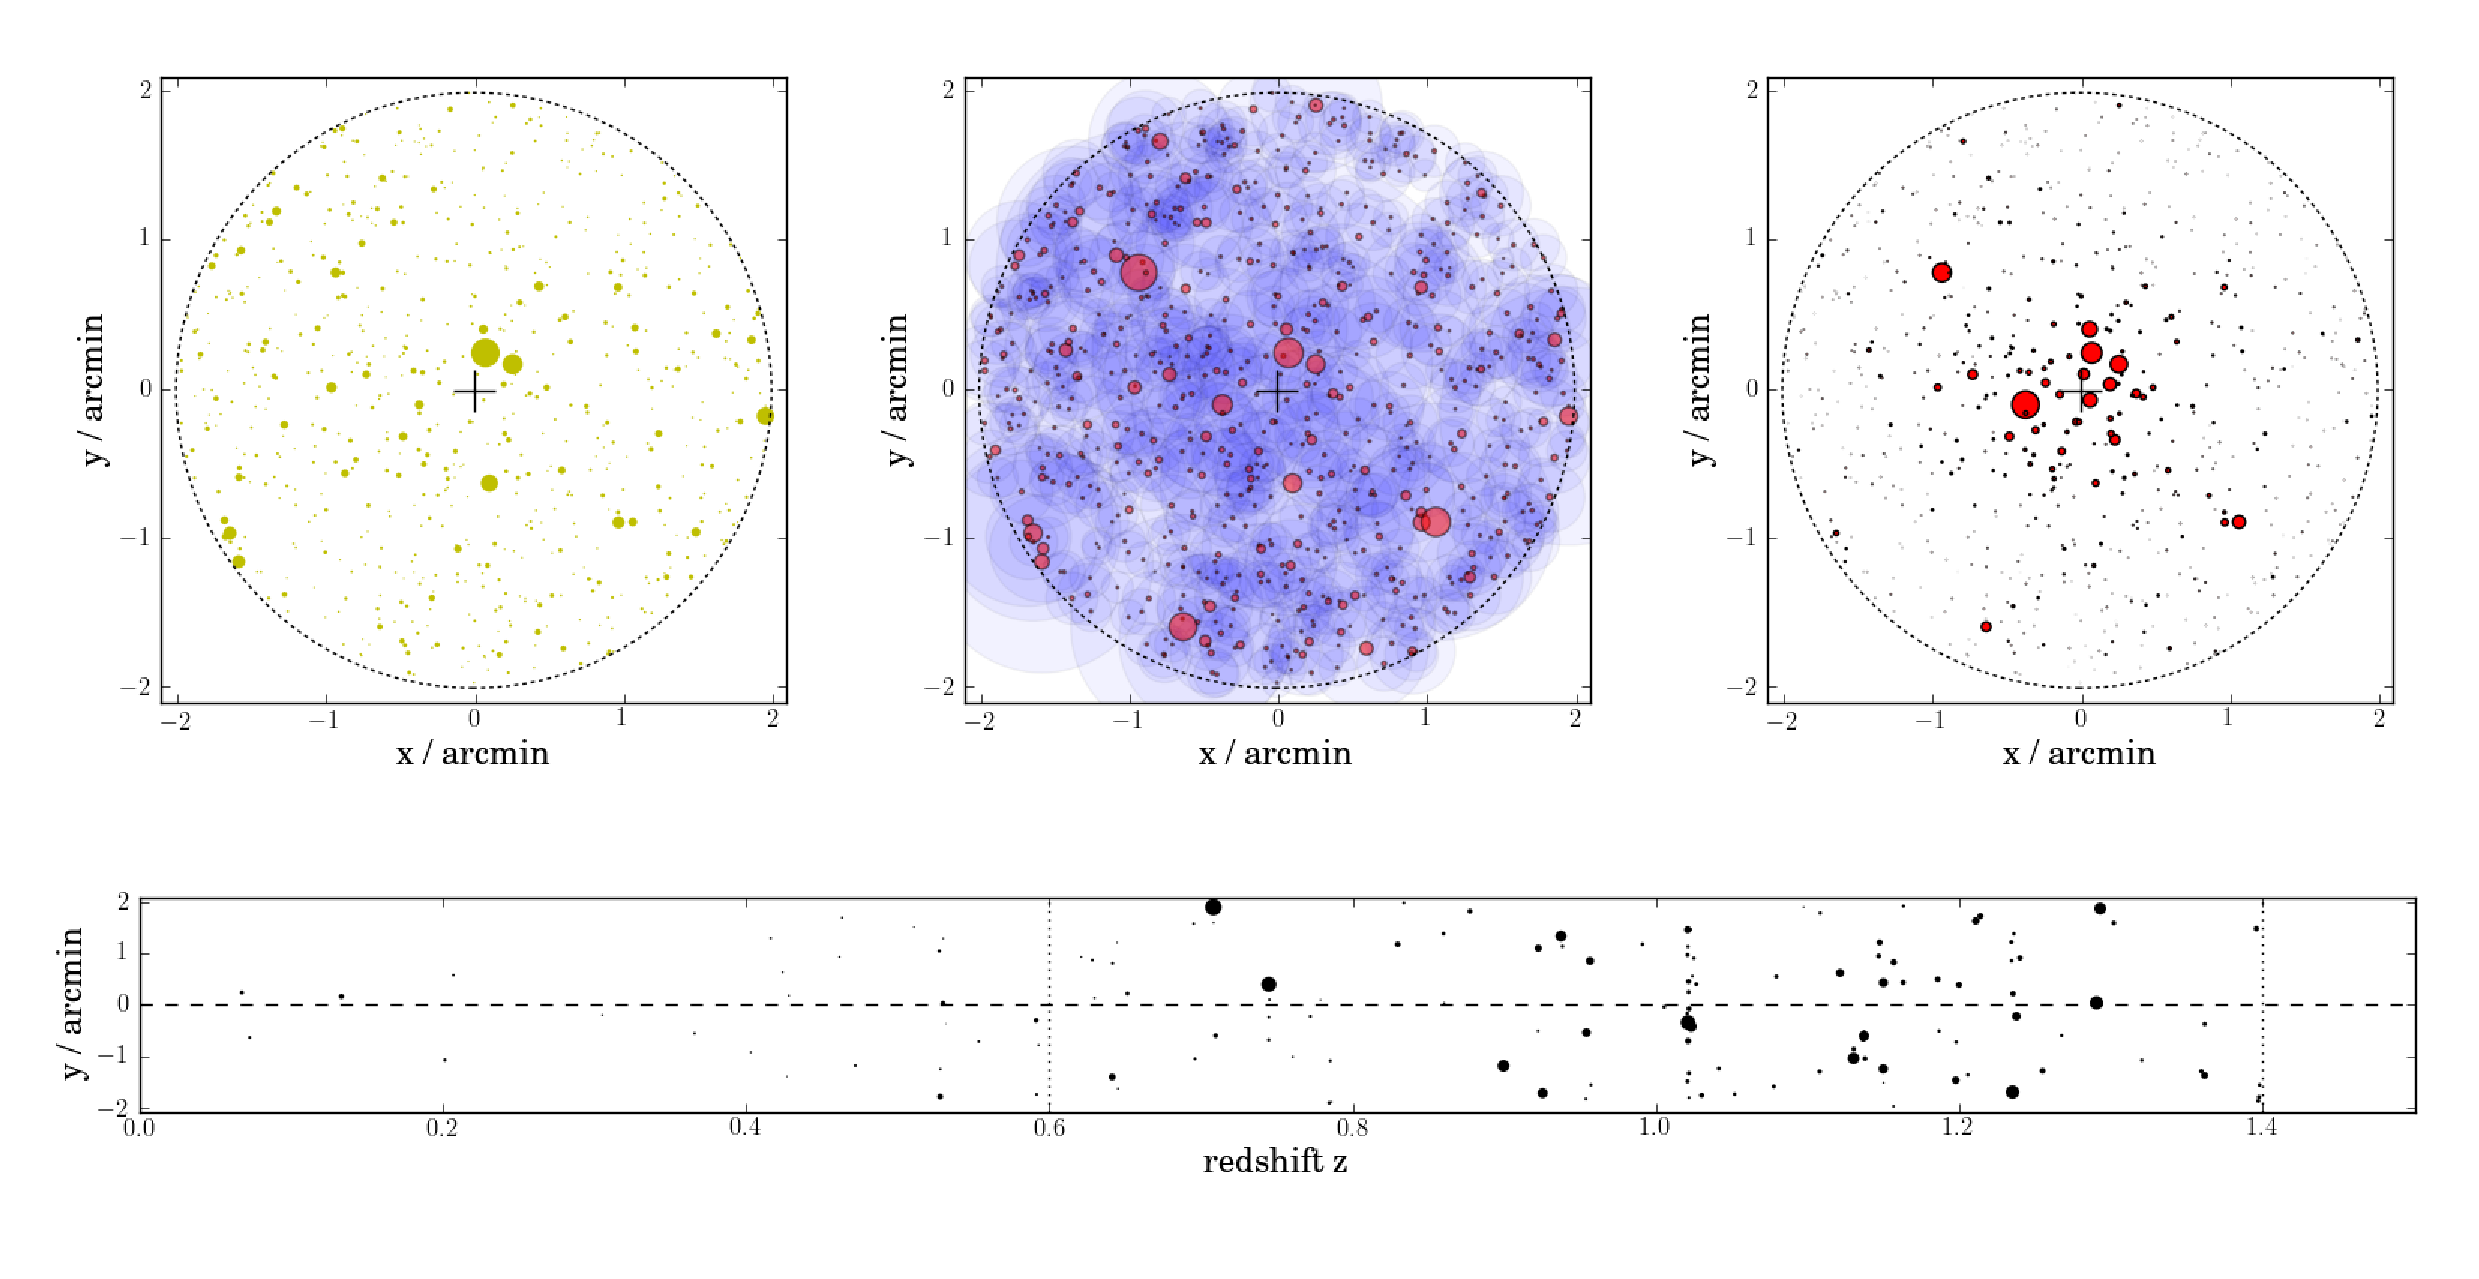
\includegraphics[width=\textwidth]{figs/viewofalightcone.eps}
\caption[magcut]{Four different views of a slightly over-dense \MS line
of sight, with a $\kappax$ of 0.03. 
{\it Top row, left:} The positions of galaxies projected on the sky. The area
of the circles is proportional to observed $i$-band flux; the brightest
object shown has an $i$ magnitude of 17.7. 
{\it Top row, centre:} The angular sizes of halos projected on the sky.
Red and blue regions lie within the NFW scale radius and virial radius
of each halo, respectively. There are essentially no empty lightcones. 
{\it Top row, right:} The individual $\kappax$ contributions of
each halo, assuming a \citet{BMO} truncated NFW 
profile and the \citet{Neto2007}
mass-concentration relation. Comparison of
this panel and the centre panel illustrates the relative importance of
proximity to the line of sight.
{\it Bottom:} A view along the redshift axis, showing only halos with
$|x|<0.3$ arcmin. The area of the points is proportional to each halo's
mass: the most massive halo shown has $1.6\times10^{12}\Msun$. The
optical axis is shown by the dashed line, while the dotted lines mark
the lens and source planes for a B1608-like strong lens.}
\label{fig:lightcone}
\end{figure*}



%%%%%%%%%%%%%%%%%%%%%%%%%%%%%%%%%%%%%%%%%%%%%%%%%%%%%%%%%%%%%%%%%%%%%%%%%%%%%%

\section{Theoretical Background}
\label{sec:theory}

\comments{
Convergence, or Ricci focusing, occurs when a gravitational lens focuses
the rays in a given bundle. This focusing can cause distant objects to
appear brighter, and larger than they would if the lens were removed.
The convergence from an isolated mass sheet is the ratio of the projected surface
mass density ($\Sigma$) \devided by the
critical surface mass density at the redshift of the mass sheet
($\Sigma_{\rm cr}$),
\be
\kappax= \frac {\Sigma}
                              {\Sigma_{\rm cr}(\zd,\zs)}
\ee
where 
\be 
\label{eq:sigcrit} 
\Sigma_{\rm cr}(\zd,\zs) \equiv \frac{c^2 D_{\rm os}}{4 \pi G D_{\rm od} D_{\rm ds}}.
\ee
and the $D$'s are the angular diameter distances between the objects
referred to in the subscripts: o is the observer, d is the deflector and
s is the source. If the surface mass density of the sheet exceeds
$\Sigma_{\rm cr}$, multiple images of the source can occur, otherwise
only one image will be observed, although that image will still be
perturbed relative to the unlensed case.


Strong lensing occurs when a massive object and background source are almost perfectly
aligned along a line of sight. The light from the background source is deflected by the
lens galaxy; this deflection allows multiple images of the background source to form
at stationary points of the time delay function. For an isolated lens, the time delay
function can be calculated from
\be \label{eq:T} 
\Delta t(\bmath{\theta},\bmath{\beta}) = \frac {1}{c} \frac{D_{\rm od} D_{\rm os}}{D_{\rm ds}} (1+z_{\rm d})\, \phi(\bmath{\theta},\bmath{\beta}),
\ee
where $\bmath{\theta}$ is the observed source position, $\bmath{\beta}$ is the 
unlensed source position, $z_{\rm d}$ is the redshift of the lens, $\phi(\bmath{\theta},\bmath{\beta})$ is
the Fermat potential. The Fermat potential is given by
\be \label{eq:FP}
\phi(\bmath{\theta},\bmath{\beta})\equiv \left[\frac{(\bmath{\theta}-\bmath{\beta})^2}{2}-\psi(\bmath{\theta}) \right], 
\ee
where $\psi(\bmath{\theta})$ is the lens potential, derived from the projected dimensionless
surface mass density, $\kappa(\bmath{\theta})$, by 
\be \label{eq:psikappa}
\kappa(\bmath{\theta})=\frac{1}{2}\nabla^2\psi(\bmath{\theta}).
\ee
}


In strong lens systems where the source is time variable, the images do not 
vary simultaneously; the optical path length for each image is different due
to relativistic and geometric effects. The difference in optical path length
causes a time-delay between the light curves of each image.
\citet{FalcoEtal1985} showed that the presence of additional matter (in the
form of a mass-sheet) along the line of sight has no observable effect except
to rescale the time-delays and magnifications. As such, it is necessary to include $\kappax$ in
the lens modelling if cosmological parameters are to be estimated accurately
and precisely from observed time delays \citep{SuyuEtal2010}. 


If there is external convergence present that is not included in the
lens modelling, then the time delay distance -- inferred assuming $\kappax
= 0$ -- will be $(1-\kappax)$ more than the true value of the time-delay distance $\Dt$:
\be 
\label{eq:MassSheet:Dtbias}
\Dt^{\rm{true}}=\frac{\Dt^{{\kappax = 0}}}{1-\kappax}.
\ee

We can hence estimate the true distance {\it only} if we have additional
knowledge of $\kappax$. Since $\kappax$ is typically small the absolute
uncertainty on the estimate of $\kappax$ corresponds to the fractional
uncertainty with which time-delay distances can be \infered.

Dynamical observations of the lens galaxy
can help break the mass-sheet degeneracy by providing an additional
estimate of the lens's mass
\citep[e.g.,][]{KoopmansEtal2003,Koopmans2004,SuyuEtal2010}. This constraint 
is useful in excluding the high convergence tails that are often present in 
PDFs for convergence - we do not include dynamical constraints in our analysis. 

In this paper we restrict ourselves to reconstructing
the line of sight portion of the mass distribution in any given field, {\it our lines of sight do not include a strong lens} which allows us to work in the weak lensing regime.  


The impact of weak-lensing perturbations on strong lensing lines-of-sight is
postponed to further work.

%%%%%%%%%%%%%%%%%%%%%%%%%%%%%%%%%%%%%%%%%%%%%%%%%%%%%%%%%%%%%%%%%%%%%%%%%%%%%%

\section{The Millennium Simulation}
\label{sec:MS}

In order to test the accuracy of our convergence estimates, we need to
know the true convergence for each line of sight. We cannot use  real
lines of sight for this,  but must use simulated lines of sight instead.
In this section we briefly review the Millennium Simulation, the ray
tracing calculations that have been carried out in it, and the mock
galaxy catalogues that have been produced.

The \MS \citep{SpringelEtal2005} is a cosmological N-body simulation of
Dark Matter structures in a cubic region approximately 680~Mpc in
co-moving size, followed from redshift 127 to the present day. With an
approximate halo mass resolution of $2\times10^{10}{\rm M}_{\odot}$
(corresponding approximately to a galaxy with luminosity $0.1L^{*}$), it
provides a detailed prediction for the distribution of dark structures
present in the Universe, under the assumptions of the $\Lambda$CDM model
of hierarchical structure formation, cosmological densities as given at
the end of \Sref{sec:intro}, and $\sigma_8 = 0.9$.
Galaxy properties,
such as stellar masses, luminosities and colours, were assigned to the
simulated halos according to a semi-analytic model for galaxy formation
\citep{DeLucia+Blaizot2007}: the resulting predictions for the galaxy
luminosity function and correlation function match the observational
data very well.

% % % % % % % % % % % % % % % % % % % % % % % % % % % % % % % % % % % % % % % 

\subsection{Convergence from Ray Tracing}
\label{sec:MS:raytracing}

\citet{HilbertEtal2009} calculated the lensing convergence using the
``lightcone'' dark matter only  output of the \MS, providing 1.7 degree
square  mock sky maps of this quantity. In this process, the dark matter
density from the simulation was projected onto a set of lens planes at
discrete redshifts, adaptively gridded and smoothed, and then the second
derivatives of the  lensing potential required for the components of the
magnification matrix were computed using a multiple lens plane ray tracing
algorithm. The first order approximation to this algorithm \citep[equation 17
of][]{HilbertEtal2009} gives the total convergence at a given sky
position~$\bmath{\theta}$ as the simple summation of the surface density in
each lens plane, weighted by the inverse critical surface density $\Sigma_{\rm
cr}$ for that plane's redshift:
\be
\kappax(\bmath{\theta}) = \sum_i \frac{\Sigma_i(\bmath{\theta})}
                                     {\Sigma_{\rm cr}(z_i,\zs)}.
\ee
\citet{HilbertEtal2009} found that this approximation is accurate to a percent level
in $\kappax$, even on 30 arcsecond scales. This accuracy sufficient for our analysis, but 
the approximation may need re-visiting in future work.

To define a test line of sight, we draw a random sky position from
within the convergence maps, bi-linearly interpolate between the pixels
of the map, and store the result as the ``true'' convergence for that
line of sight, $\kappax^{\rm true}$. 


\new{The adaptive smoothing of the matter in the \MS results in a spatial resolution of $\sim 5\,\text{kpc}$ comoving in the densest regions, and $\sim10\,\text{kpc}$ on average. This resolution is sufficient to capture most of the variance in the convergence \citep{TakahashiEtal2011}. Moreover, we seek to estimate the component of the convergence that is smooth on the angular scales of typical strong galaxy-scale lens systems ($\sim 1\,\text{arcsec}$). Any variations of the external convergence on smaller scales can be directly recovered from the resulting image distortions in the lens modelling.}


\comment{PJM: This means our sightlines are not typical of strong lenses, because they
don't include the local overdense region typically found near massive lens
galaxies. Our lines of sight have typical mass distributions for a lens line
of sight {\it after excision of the lens plane}. I have tried to explain
this above.}

% % % % % % % % % % % % % % % % % % % % % % % % % % % % % % % % % % % % % % % 

\subsection{Mock Photometric Galaxy Catalogues}
\label{sec:MS:mocks}

We construct mock photometric galaxy catalogues by selecting all \MS galaxies
within a circular aperture of a given angular radius centred on each randomly
selected line of sight position, with apparent $i$-band magnitude brighter
than a given limit. The parent catalogue, from \citet{HilbertEtal2011},
contains galaxy positions and magnitudes, all of which include lensing effects
(deflections and magnifications). We also have access to the underlying galaxy
halo masses and redshifts, which we will use to calibrate the reconstruction,
and also to explore any sources of bias and scatter. Since the ``true''
convergence is that of only the dark matter, we focus on reconstructing the
dark matter halos alone. Our model for doing this is outlined in the next
section. 

%%%%%%%%%%%%%%%%%%%%%%%%%%%%%%%%%%%%%%%%%%%%%%%%%%%%%%%%%%%%%%%%%%%%%%%%%%%%%%

\section{Estimating Convergence: The Halo Model Approximation}
\label{sec:model}

We require a method for estimating the convergence at any point on the sky,
given a catalogue of observed galaxy properties such as positions,
brightnesses, colours, and possibly stellar masses and redshifts, for every
galaxy in the field of the lens, down to some magnitude limit. Since we cannot
observe the surface mass density of each halo directly, we need some way of
estimating the mass of each halo in the catalogue, so that we can compute its
contribution to the total $\kappax$ along the line of sight \citep[as in
\eg][]{GunnarssonEtal2006,KarpenkaEtal2012}.  This mass
assignment recipe will be uncertain, and also incomplete, but it can be
calibrated with cosmological simulations, which represent a significant
additional source of information to what is present in the data.

Transforming an observed photometric galaxy catalogue into a  catalogue of
halo masses, positions, and redshifts will enable us to attempt a
reconstruction of the convergence induced by every halo near a line of sight. 
We also need to account for the convergence due to dark structures and the
divergence due to voids; we do not model voids or dark structures, but their
effects are included statistically by calibrating the convergence in
halos, $\kappah$, against the ray-traced convergence, $\kappax$, for \MS lines
of sight.


% % % % % % % % % % % % % % % % % % % % % % % % % % % % % % % % % % % % % % % 

\subsection{Halos}
\label{sec:model:halos}

Cosmological dark matter simulations have shown that dark matter
halos are reasonably well-approximated by NFW profiles 
\citep{NFW}. We assume each halo to have a spherical mass distribution with 
density given by
\be\label{eq:rhonfw}
\rho(r) = 
\frac{\rho_0}{\left(r/r_{s}\right)
\left(1+r/r_{s}\right)^{2}}.
\ee
Here, $r_{s}$ is a characteristic scale 
radius of the cluster, representing the point where
the density slope transitions from $r^{-1}$ to $r^{-3}$. This radius is
related to the virial radius of the halo by $r_{s}~=~r_{200}/c$, where $c$ is
the concentration parameter, which can be estimated from the halo's mass,
using a mass--concentration relation. Typically more massive halos are less
concentrated, but there is some scatter; we use the relation of
\citet{Neto2007} to estimate $c$ from the mass enclosed within $r_{200}$,
which we denote as $M_{200}$. We find our results do not change if the
\citet{MaccioEtal2008} mass--concentration relation is used instead. 

If one integrates the density profile of an NFW profile out to infinite
radius, the total mass diverges. Similarly, if the universe is
homogeneously populated with NFW halos, the projected surface mass along
any line of sight will also be divergent.\footnote{At large radius,
$\Sigma_{\rm nfw} \propto R^{-2}$, but the differential number of halos
centred within an annulus of width $\dee R$ is given by $\dee N_{\rm
annulus} \propto R \dee R$, so  $\Sigma_{\rm total} \propto
\int_{0}^{\infty} R^{-1} \dee R$, which diverges logarithmically} Since
infinite mass is unphysical, the profile must be truncated at some
point. Several truncation profiles have been suggested
\citep[e.g][]{BMO}, but beyond several virial radii, the amount of
matter associated with a halo is likely to be low. In this work we
assume the truncated NFW profile
\be\label{eq:bmoprofile}
\rho(r) = 
\frac{\rho_{\rm NFW} (r)}{1+\left(r/r_{t}\right)^2},
\ee
which is the same as the NFW profile in the limit that the truncation
radius, $r_t$ goes to infinity; the shear and convergence from such a
profile are derived in \citet{BMO}.
 We use a truncation radius of five times
the virial radius, but our results are robust for any choice of $r_t>2
\times r_{200}$. 

Many studies have shown that galaxies have total mass density profiles that
are approximately isothermal in their inner regions
\citep[\eg][]{AugerEtal2010} due to the more concentrated stellar mass
component.
This has been confirmed by galaxy-galaxy weak lensing measurements 
\citep[\eg][]{Mandelbaum,GavazziEtal2007}. We note that the two halo term that
dominates the galaxy-galaxy lensing signal at large radii is explicitly taken
into account in our model, where every galaxy is assigned a dark matter halo.
At large radii an NFW-like profile is probably appropriate, but may not be
correct when a halo is very close to the line of sight.


Each halo in our catalogue contributes to
the line of sight convergence by
\be
\label{eq:kappai}
\kappa_i =\Sigma_{i}/\Sigma_{\mathrm{cr}}(z_i,\zs),
\ee
where $\Sigma_{\mathrm{cr}}(z_i,\zs)$ is the critical surface density \comments{was defined in \Eref{eq:sigcrit}}.
Following the first order approximation of \citet{HilbertEtal2009}
outlined in \Sref{sec:MS} above, we compute 
the total convergence from all the halos along the line
of sight using
\be 
\label{eq:kappasummu}
\kappah = \sum_{i} \kappa_i.
\ee

To estimate a halo's contribution to $\kappah$ we must first know the
halo's mass \new{and position. The stellar mass
and host halo are not necessarily concentric, especially for central
galaxies of giant clusters, but our reconstruction assumes the dark matter halo is centred on
the visible galaxy.} For the lines of sight of the \MS, halo masses are
known, but for  real lines of sight the halo masses have to be \infered
from whatever data are available. 
In this work we investigate the use of the empirical stellar mass --
halo mass relation for this purpose. The primary advantage of this
approach is that it is a simple, ``one size fits all'' relation that can
be applied regardless of the stellar mass observed. We discuss
additional observables that could be used to improve the precision of
the halo mass inference in \Sref{sec:discuss} below. 

We use the relation of \citet{BehrooziEtal2010} to infer halo masses
from stellar masses; the details of this \proceedure are outlined in 
\Aref{appendix:MSMH}. Given an uncertain stellar mass and redshift for
each galaxy in the  catalogue, we draw a sample halo mass from the PDF
that describes this uncertainty (\Eref{eq:mhalo-mstar}) and use
\Eref{eq:kappai} to compute its contribution to the convergence,
$\kappa_i$; this can be done for all the halos along a specific line of sight
and summed to give a sample value of $\kappah$;  repeatedly applying
this \proceedure allows us to build up a histogram of $\kappah$ values
consistent with the data, and hence characterize $\pr(\kappah|\data)$. 

This PDF contains a hidden assumption of an uninformative prior PDF for
$\kappah$ -- in the case of infinitely poorly measured stellar masses and
redshifts, $\pr(\kappah|\data)$ will have very long tails corresponding to
very over-dense lines of sight that we do not believe exist. The resolution of this
is to divide out the effective prior PDF that was applied during the halo mass
estimation process (which is broad, and hence close to uniform), and apply an
additional prior on $\kappah$, given by the global underlying $\kappah$
distribution from the simulation. In the limiting  case of very poor
photometric data, $\pr(\kappah|\data)$ then defaults to this distribution, as
required.

% \todo{All}{Discuss this. It ties us to the simulation, but only weakly. Is the
% argument about poor data valid? Tom?}

% TEC: yes it's valid. It only really ties us to the halo mass function of the
% simulation. It's probably tied at the same level as the "global P(\kappa) as
% derived from Stefan's ray-tracing"


% % % % % % % % % % % % % % % % % % % % % % % % % % % % % % % % % % % % % % % 

\subsection{Accounting for voids, filaments and other dark structures}
\label{sec:model:voids}

Our halo model accounts for the convergence contribution of density
perturbations that can be associated with light. Filaments and dark
substructures contribute additional convergence, while voids contribute a
divergence; these structures must be included to produce an unbiased estimate
of $\kappax$. In particular, neglecting voids would lead to a heavily biased
estimate of $\kappax$, since the halo model's $\kappah$ can only be positive.
In principle the absence of galaxies implies something about the presence of a
void, but we do not currently attempt to use this information. In general, it
is difficult to account for the unseen mass, since we do not have a good model
for its density structure.

The solution we present here is to calibrate the relationship between the halo
convergence $\kappah$ and the overall convergence $\kappax$ (as would be
calculated by ray tracing through the full density field)  using the
simulations themselves. The halo modelling procedure outlined in
\Sref{sec:model:halos} allows  us to estimate  the convergence due to halos
given observations of  mass, redshift and position,
$\pr(\kappah|\data)$, but what we are interested in is the total
convergence along the line of sight $\pr(\kappax|\data)$. We can obtain
this by considering the expression: 
\begin{equation} 
\Pr(\kappax|\data) = 
   \int \dee\kappah  \Pr(\kappax|\kappah,\data) \Pr(\kappah|\data)
   \label{eq:kappaconv}
\end{equation} 
The first term in the integrand relates the convergence due to model halos,
$\kappah$, to the true convergence, $\kappax$. This conditional distribution
can be constructed from the \MS catalogues, by computing
$\kappah$ from the true halo masses and redshifts 
along each selected line of sight, and then
accumulating $\kappah$, $\kappax$ pairs
for a large number of such sightlines. 
For any given line of sight we can then estimate
$\pr(\kappah|\data)$ as described above, and then multiply it by
$\Pr(\kappax|\kappah)$ and integrate out the intermediate parameter
$\kappah$. 

\phil{However, if the conversion between stellar mass and halo mass is very
uncertain, $\pr(\kappah|\data)$ is shifted relative to what it would
have been given perfect knowledge of the halo masses.  This is because the
conversion from stellar mass to halo mass and into $\kappah$ is highly
asymmetric: a long tail of high halo masses gives rise to a tendency to
overestimate $\kappah$. If this shift is ignored, the resulting
$\Pr(\kappax|\data)$ will be systematically biased towards high values of
$\kappax$. Instead, we need the  distribution of $\kappax$ from all
calibration lines of sight that have a $\pr(\kappah|\data)$ that is identical
to the $\pr(\kappah|\data)$ for the real line of sight {\it given the same
data quality}; however, we found this approach unfeasible  given our finite
number of calibration lines of sight. A working compromise is to use 
the median of the $\pr(\kappah|\data)$ distributions in the calibration.}

We  take a large number of
calibration lines of sight from the \MS catalogues and generate a mock
stellar mass catalogue for each one. We then reconstruct each lightcone in the
same way as we would an observed field,
estimate $\pr(\kappah|\data)$, and extract its median. Accumulating
these median values $\kappah^{\rm med}$ and 
their corresponding true values of $\kappax$, we can form the 
conditional distribution $\pr(\kappax|\kappah^{\rm med})$. 
Then, to infer $\kappax$ from an observed photometric catalogue, we 
estimate $\pr(\kappah|\data)$ 
using the halo model, compute the median value 
$\kappa_{\rm h,obs}^{\rm med}$, and then use a modified
version of 
\Eref{eq:kappaconv} to infer $\kappax$: 
\bea
\Pr(\kappax|\kappah^{\rm med},\data) &=& \int \dee\kappah^{\rm med} 
   \Pr(\kappax|\kappah^{\rm med},\data) \Pr(\kappah^{\rm med}|\data) \notag \\
\label{eq:calkappaconv}   
\eea
\phil{This integral is trivial, since $\Pr(\kappah^{\rm med}|\data)$ is
a delta function centred on the median of the inferred PDF for $\kappah$.
However,}
because we only have a finite number of calibration lines of sight, we use all
calibration lines of sight with $\kappa_{\rm h,cal}^{\rm med} =
\kappah^{\rm med}\pm0.003$ to form $\Pr(\kappax|\kappah^{\rm
med},\data)$.
\comments{, with each calibration sightline weighted equally. PJM: why is
this? Surely one should weight by the value of the Gaussian function implied
by that ``$\pm 0.003$''?}

This procedure of reducing the full PDF for $\kappah$ to its median increases
the importance of the realism of the simulation: the simulation needs to be as
similar as possible to the real universe or there is a possibility of
systematic errors. Conversely, making use of all the information
in the photometric catalogue yields $\kappax$ estimates of increased
precision.

%%%%%%%%%%%%%%%%%%%%%%%%%%%%%%%%%%%%%%%%%%%%%%%%%%%%%%%%%%%%%%%%%%%%%%%%%%%%%%

\section{Results: Perfect Halo Data}
\label{sec:knownMh+z} 

We now put the reconstruction \proceedure outlined above into practice, first
inferring $\kappax$ from $\kappah$ in the case of hypothetical galaxy
catalogues with noiseless redshifts and halo masses. The reason for doing this
is to check the validity of the calibration process, and then also to 
investigate the primary sources of the convergence. It will also provide us
with a measure of the intrinsic uncertainty introduced by our assumptions of
all illuminated halos being spherically-symmetric truncated NFW halos following the
Neto et al concentration--mass relation \new{and of visible galaxies being concentric with their host halos}.

% % % % % % % % % % % % % % % % % % % % % % % % % % % % % % % % % % % % % % % 

\subsection{How is $\kappah$ related to $\kappax$?}

\Fref{fig:jointkh-k} shows the conditional distribution of $\kappax$ given 
$\kappah$, derived from $10^5$ randomly selected \MS lines of sight
and assuming noise-free halo masses and redshifts. 
\phil{In this case, $\pr(\kappah|\data)$ is almost a delta function since the only uncertainty is halo
concentration, which has minimal effect on $\pr(\kappah|\data)$.  
}
% In this case, the PDF : we can read
% off  $\pr(\kappax|\data)$ just by taking a thin vertical slice through this 
% distribution. 
% Note that the joint PDF plotted in this figure is the product
% of  the conditional distribution that we need for calibration, and also the
% prior PDF for $\kappah$ that we need to ensure that the global distribution of
% $\kappah$ values is defaulted to in the case of poor observational data. 
At fixed $\kappah$ we find in \Fref{fig:jointkh-k} that the scatter in 
$\kappax$
grows with $\kappah$; our reconstruction is better at reproducing under-dense
lines of sight than over-dense lines of sight. The effect of ignoring voids
and the smooth mass component is evident in this plot: $\kappah$ is
significantly higher than $\kappax$, at any given $\kappax$ value. 
\phil{Conditioning on $\kappah$ gives a PDF for
$\kappax$ centred at the correct place, by construction.}

%%%%%%%%%%%%%%%%%%%%%%%%%%%%%%%%%%%%
\begin{figure}
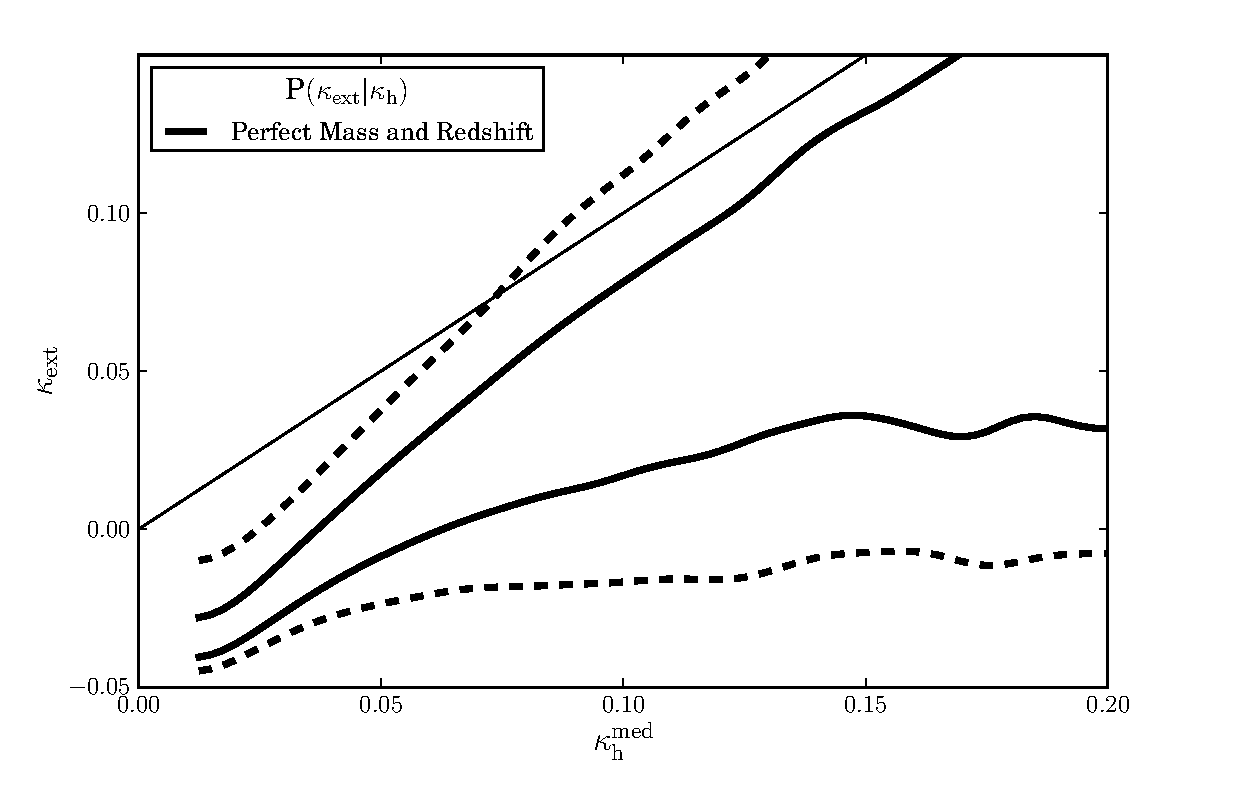
\includegraphics[width=\columnwidth]{figs/cornerplot.eps}
\caption[Biased?]{The conditional distribution of 
$\kappax$ given $\kappah$, in the case where  
we have perfect knowledge of halo mass and redshift.
$10^5$ reconstructed lines of
sight were used to make this plot. 
Solid (dashed) lines enclose 68\% (95\%) of the conditional probability.
$\kappah$ traces $\kappax$, but with a positive offset which arises from
$\kappah$ not accounting for any voids or dark structures.
At fixed $\kappah$ the scatter in $\kappax$ grows rapidly with $\kappah$.
\tom{The thin diagonal line follows $\kappax=\kappah$.}}
\label{fig:jointkh-k}
\end{figure}
%%%%%%%%%%%%%%%%%%%%%%%%%%%%%%%%%%%%


% % % % % % % % % % % % % % % % % % % % % % % % % % % % % % % % % % % % % % % 

\subsection{How accurate is the $\kappah - \kappax$ calibration?}

%%%%%%%%%%%%%%%%%%%%%%%%%%%%%%%%%%%%
\begin{figure}
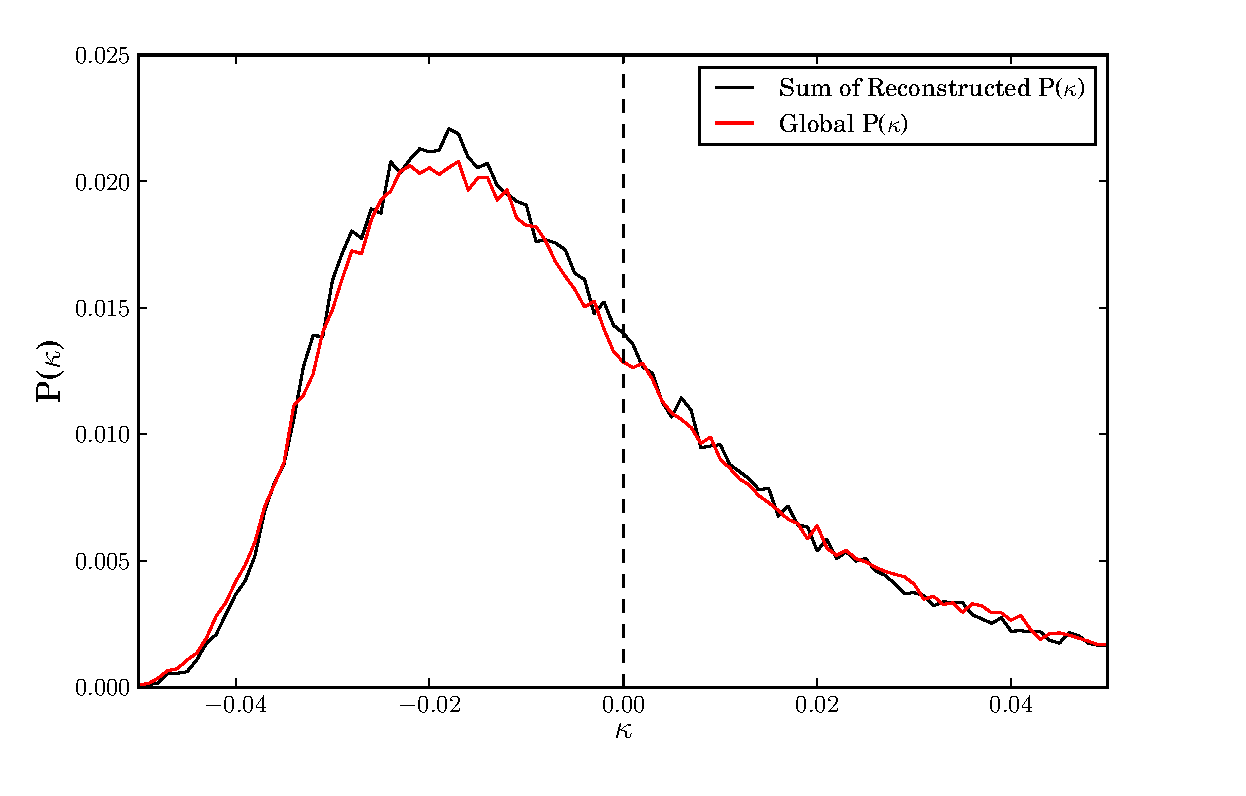
\includegraphics[width=\columnwidth]{figs/globaldist.eps}
\caption[magcut]{Recovering the global $\pr(\kappax)$ (shown in red). The
black curve shows a histogram of  inferred  $\kappax$ values from $10^{5}$
reconstructed lines of sight.  The reconstructions were performed given
perfect knowledge of halo mass and redshift -- in this case the reconstruction
recovers the correct convergence.}
\label{fig:globaldist}
\end{figure}
%%%%%%%%%%%%%%%%%%%%%%%%%%%%%%%%%%%%

%%%%%%%%%%%%%%%%%%%%%%%%%%%%%%%%%%%%
\begin{figure*}
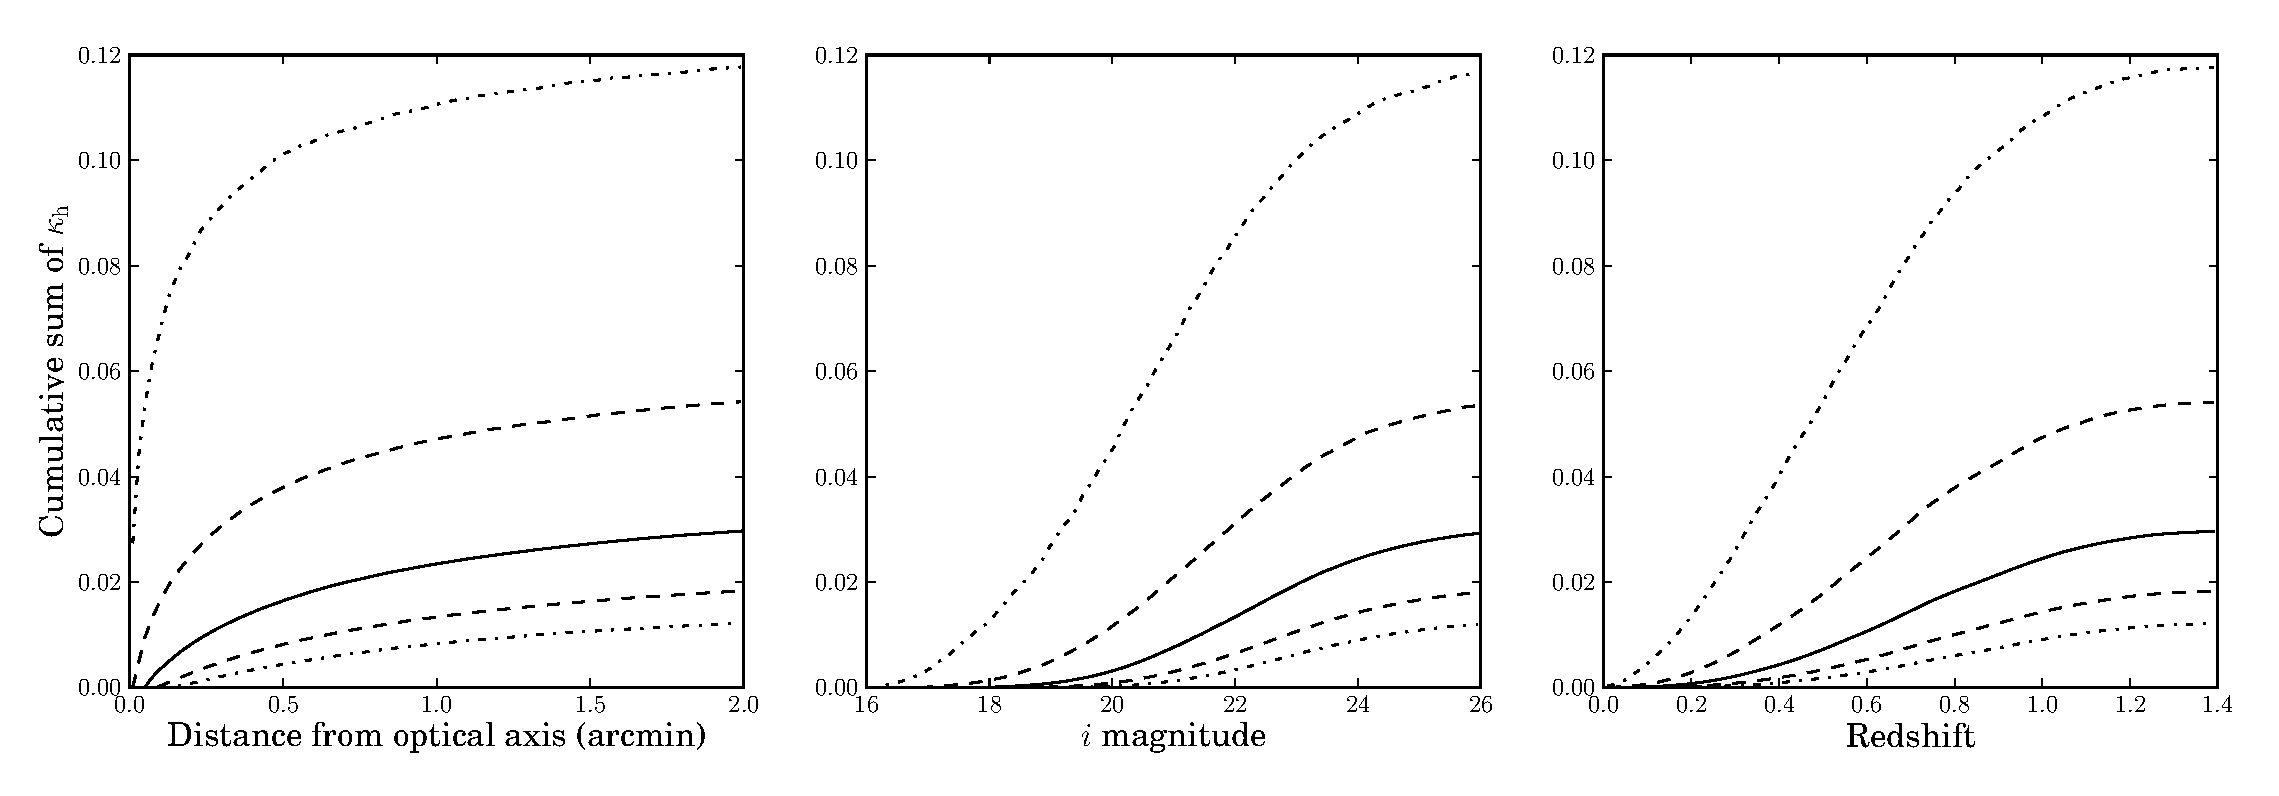
\includegraphics[width=\textwidth]{figs/where_is_the_kappa.eps}
\caption[magcut]{Which objects dominate the external convergence for a line of
sight? From left to right, the three figures show the cumulative contribution
to the total convergence from individual halos ($\kappah$) as a function of
1) distance from the line of sight, 2) magnitude and 3) redshift.   In each
panel, the solid line is the median cumulative contribution over a large
sample of lines of sight, while dashed and dot-dashed show the ranges enclosing 68
and 95 percent of the lines of sight respectively. The source is at redshift 1.4.}
\label{fig:where}
\end{figure*}
%%%%%%%%%%%%%%%%%%%%%%%%%%%%%%%%%%%%

Let us define the ``bias'' of the reconstruction of a given line of sight as
the difference between the expectation value of $\kappax$ over its posterior
PDF $\pr(\kappax|\data)$ and the known true value $\kappax^{\mathrm{true}}$.
Let us also define the ``width,'' $\sigma_{\kappa}$, to be half the width of
the interval containing the central $68\%$ of the posterior probability
$\pr(\kappax|\data)$. 

In an ensemble of $10^{5}$ reconstructed lines of sight, we find the mean bias
to be $-1\times 10^{-5}$, and the mean width to be 0.01. This is
1.8 times smaller than the width of the global $\pr(\kappax)$.  We find that
our inferred $\kappax$ PDFs are consistent with the global $\kappax$
distribution; \Fref{fig:globaldist} shows that sampling from the
$\pr(\kappax|\data)$ inferred from reconstructions of  $10^{5}$ lines of
sight  produces a distribution of $\kappax$ values over the sky nearly identical to
the global $\pr(\kappax)$. Given perfect knowledge of halo mass and redshift
then, the calibration \proceedure provides an unbiased estimate of $\kappax$
that is $1.8$ times more precise than using the global $\pr(\kappax)$. 
\phil{This is the maximum precision we can obtain using the current calibrated
halo model.}

% % % % % % % % % % % % % % % % % % % % % % % % % % % % % % % % % % % % % % % 

\subsection{Which halos dominate the $\kappah$ distribution?}

Before investigating the impact of imperfect knowledge of halo
mass and redshift, we investigate the uncertainties induced by limits on the
magnitude of the observed galaxy sample, and on the field of view. The halos
in our catalogue are populated by galaxies and given magnitudes according to
the semi-analytic model of \citet{DeLucia+Blaizot2007}: by applying magnitude
cuts to our catalogue, we can investigate the amount of scatter caused by
unobserved halos. 

\Fref{fig:where} shows the cumulative contribution to $\kappah$ as a function
of projected distance from the line of sight, magnitude and redshift. We find
that most of the convergence comes from halos close to the line of sight. 
Over half of the  convergence typically comes from halos within 30 arcseconds
of the line of sight; by 2 arcminutes, this fraction is 85\%. The contribution
from halos beyond 2 arcminutes is relatively constant at a contribution of
0.008$\pm$0.003. We find that ignoring halos beyond 2 arcminutes has no effect
on the precision of the reconstruction; this is shown in \Fref{fig:radcut}. As
a function of magnitude, we find that $\kappah$ is dominated by objects with
magnitudes between $i=18$ and $i=24$. Objects brighter than $i=18$ are either
too rare, or too close to the observer, to make a significant contribution to
the convergence. Objects fainter than $i=24$ are too small to be important,
unless they are extremely close to the line of sight; we find that
including halos fainter than $i=24$ does not improve the reconstruction. 
\Fref{fig:magcut} shows the scatter on $\kappah-\kappax$ (where $\kappah$ is
shifted so that its mean is zero, \phil{to emulate the effect of the eventual
calibration}) as a function of reconstruction magnitude limit. We do not
expect a deeper survey to decrease the size of the uncertainty in mapping
$\kappah$ onto $\kappax$. Halos at all redshifts out to the source redshift
(1.4 in this work. The redshift of the source in B1608+656) contribute to the convergence, but the largest contribution comes
from halos with $z \sim z_{\rm source}/2$.

%%%%%%%%%%%%%%%%%%%%%%%%%%%%%
\begin{figure}
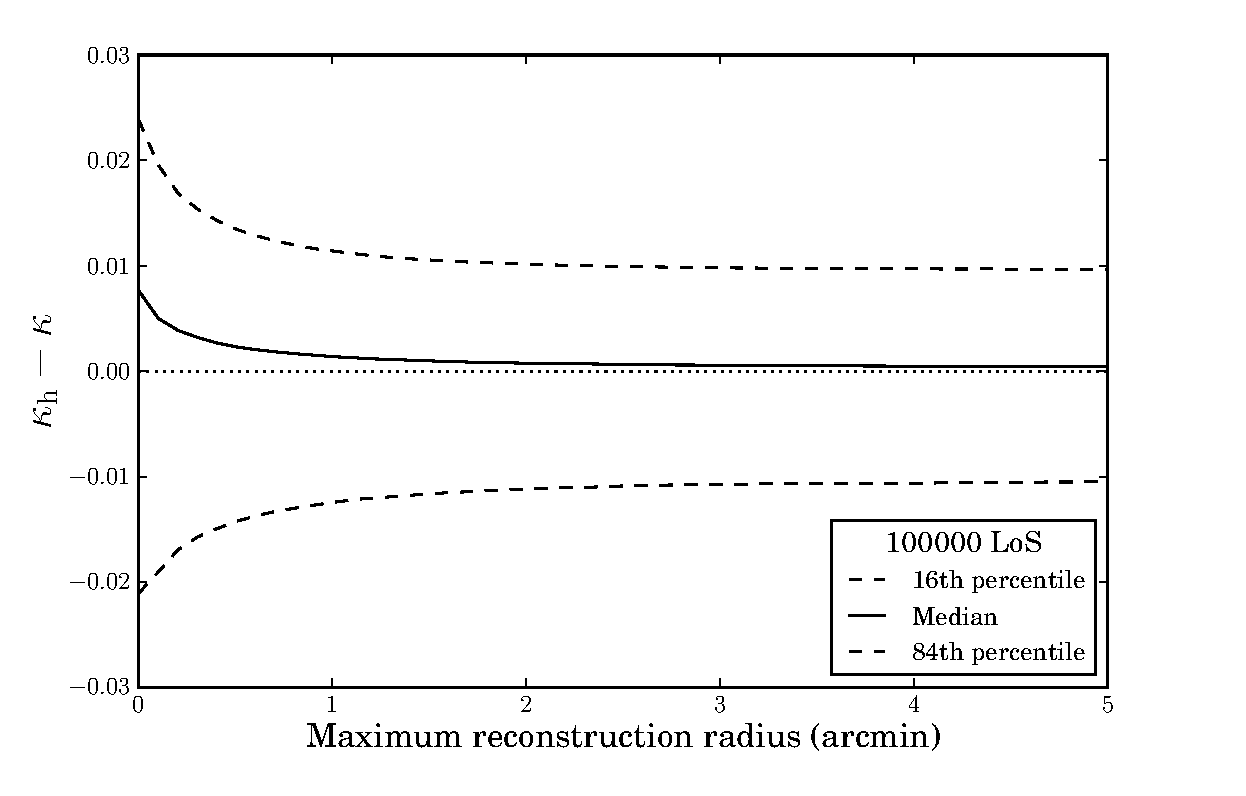
\includegraphics[width=\columnwidth]{figs/radius_scatter.eps}
\caption[magcut]{The 16, 50 and 84th percentiles of $\kappah$ minus
$\kappax$ as a function of the limiting radius of the halo
reconstruction. $\kappah$ has been shifted such that
$\left\langle\kappah\right\rangle=0$ \phil{to emulate the effect of the
eventual calibration}. 
The majority of the constraining power
comes from reconstructing halos within 2~arcmin of the line of sight.}
\label{fig:radcut}
\end{figure}
%%%%%%%%%%%%%%%%%%%%%%%%%%%%%

%%%%%%%%%%%%%%%%%%%%%%%%%%%%%
\begin{figure}
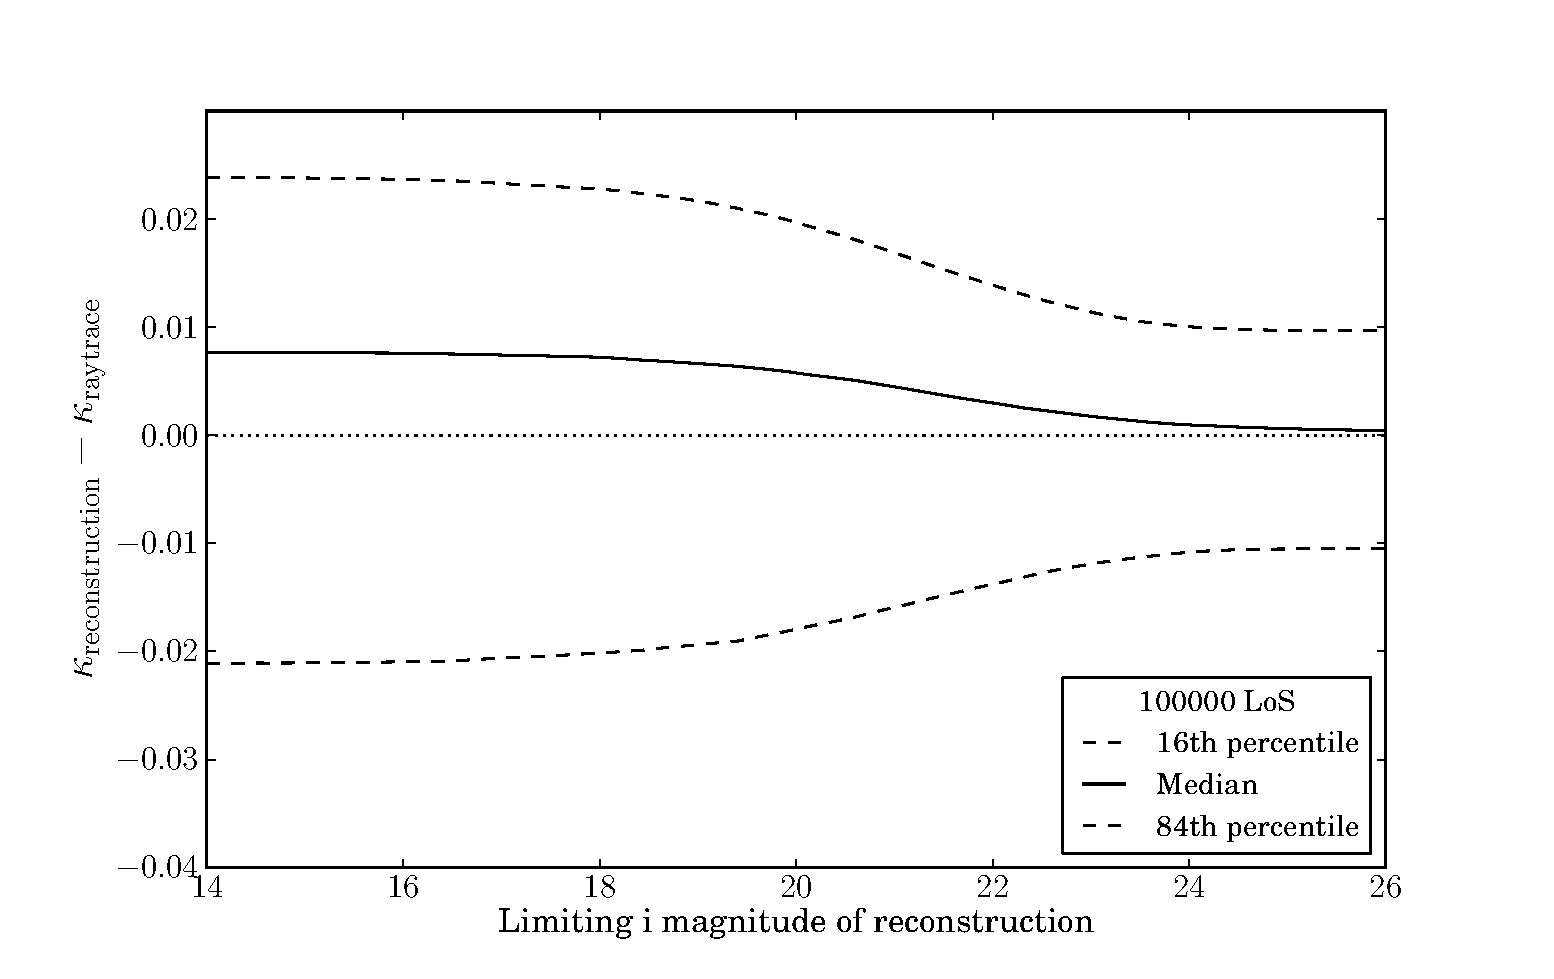
\includegraphics[width=\columnwidth]{figs/mag_scatter.eps}
\caption[magcut]{The 16, 50 and 84th percentiles of $\kappah$ minus
$\kappax$ as a function of the limiting $i$ band depth of the halo
reconstruction. $\kappah$ has been shifted such that
$\left\langle\kappah\right\rangle=0$ \phil{to emulate the effect of the
eventual calibration}. The majority of the constraining power
comes from reconstructing halos with magnitudes between $18<i<24$.}
\label{fig:magcut}
\end{figure}
%%%%%%%%%%%%%%%%%%%%%%%%%%%%%


%%%%%%%%%%%%%%%%%%%%%%%%%%%%%%%%%%%%%%%%%%%%%%%%%%%%%%%%%%%%%%%%%%%%%%%%%%%%%%%%

\section{Testing the Halo Model Reconstruction on Mock Galaxy Catalogues}
\label{sec:obsMstar+z}

We now move on to consider the halo model reconstruction of line-of-sight mass
distributions given noisy astronomical observables. A typical imaging survey
can be expected to provide measurements of the positions and magnitudes of
galaxies in a field;  spectra for some of the objects may either come from a
synergistic survey, or from targeted follow-up. In this section we quantify
the uncertainties induced by inferring the halo mass and redshift from these
observables. 

%\flag{Should we show the relevant calibration plots, analogous to Figure 2?
%Seems a bit odd to give Figure 2 but not illustrate the {\it actual
%calibration procedure we follow on real data}... Maybe we could make one that
%had the conditional distribution for each data quality?}

%TEC: I think that could lead to figure overload; the concept is given throughout
% the paper, and it's well illustrated by figure 2.

As described in \Sref{sec:model:halos}, in this work we attempt to  infer halo
masses from measurements of stellar mass. We will investigate two main sources
of uncertainty: the stellar masses themselves, and placing halos at
photometric redshifts. Much work has already focused on using photometric
colours to infer stellar mass \citep[\eg][]{AugerEtal2009} and redshifts
\citep[\eg][]{BPZ}: we will estimate the likely uncertainties on stellar mass
and redshift based on this work.  


% % % % % % % % % % % % % % % % % % % % % % % % % % % % % % % % % % % % % % % 

\subsection{Making Mock Observational Catalogues}

\phil{While the \MS catalogues do already contain stellar masses for each
galaxy, we do not use them for two reasons. The first is that at the low mass
end, the dark matter-only \MS satellite galaxy halos are highly  stripped
relative to what we might expect in a universe containing baryons, leading to
a mismatch between the observed and simulated stellar mass--halo mass
relations.  The second is that we wanted to be able to perform the functional
test of trying to recover the convergence having assumed the correct stellar
mass--halo mass relation.} For these reasons, we assign a new true stellar
mass to each halo in the \MS catalogues, according to the empirical stellar
mass--halo mass relation of \citet{BehrooziEtal2010}. \new{When assigning stellar
masses we have treated satellites in the same way as central halos; in the real
universe both the density profile and the stellar mass--halo mass relation are
likely different for satellites and centrals, but our simple model does not include
these effects}. From these we simulate
observed stellar masses by drawing samples from  $\pr(\log{M^{*}_{\rm
obs}}|\log{M^{*}_{\rm true}})$ which we take to be a Gaussian of width
$\sigma_{M_*}$ centred on $\log(M*_{\mathrm {true}})$. Where a spectroscopic
redshift exists, stellar masses can be estimated with typical uncertainties of
0.15 dex \citep{AugerEtal2009}; however with photometric redshifts stellar
mass uncertainties are typically three times as large. We use
$\sigma_{M_*}=0.15$ dex for halos with a spectroscopic redshift and
$\sigma_{M_*}=0.45$ dex otherwise. For photometric redshift uncertainties we
draw a redshift from $\pr(z_{\rm true}|z_{\rm obs})$ which we take to be a
Gaussian of width $0.1(1+z_{\rm spec})$ centred on $z_{\rm spec}$, where
$z_{\rm spec}$ is the halo's true redshift in the \MS catalogue. \new{In our mock catalogues 
we have used the galaxy position from the \MS; this is not necessarily coincident with the
centre of the galaxy's host dark matter halo.}

\comment{The following is relevant to all sections on inferring $\kappax$
given imperfect data, so it belongs here and not in the spectroscopic redshift
first subsection.}

Given an uncertain stellar mass and redshift it is possible to infer a
halo mass using the stellar mass--halo mass relation of
\citet{BehrooziEtal2010}. This \proceedure requires an inversion of the
relation given in \citet{BehrooziEtal2010} and correctly inverting the
relation's uncertainties requires care: the \proceedure we use to do this
is given in \Aref{appendix:MSMH}. By drawing sample halo masses
and redshifts, we can infer a sample $\kappah$ using the \proceedure of
\Sref{sec:model}. Repeatedly drawing samples allows us to
estimate $\pr(\kappah|\data)$ for each reconstructed line of sight. We then
transform this into our target PDF $\pr(\kappax|\data)$ as described above.


% % % % % % % % % % % % % % % % % % % % % % % % % % % % % % % % % % % % % % % 

\subsection{Reconstructing $\kappax$ given a spectroscopic redshift for every object}

%%%%%%%%%%%%%%%%%%%%%%%%%
\begin{figure}
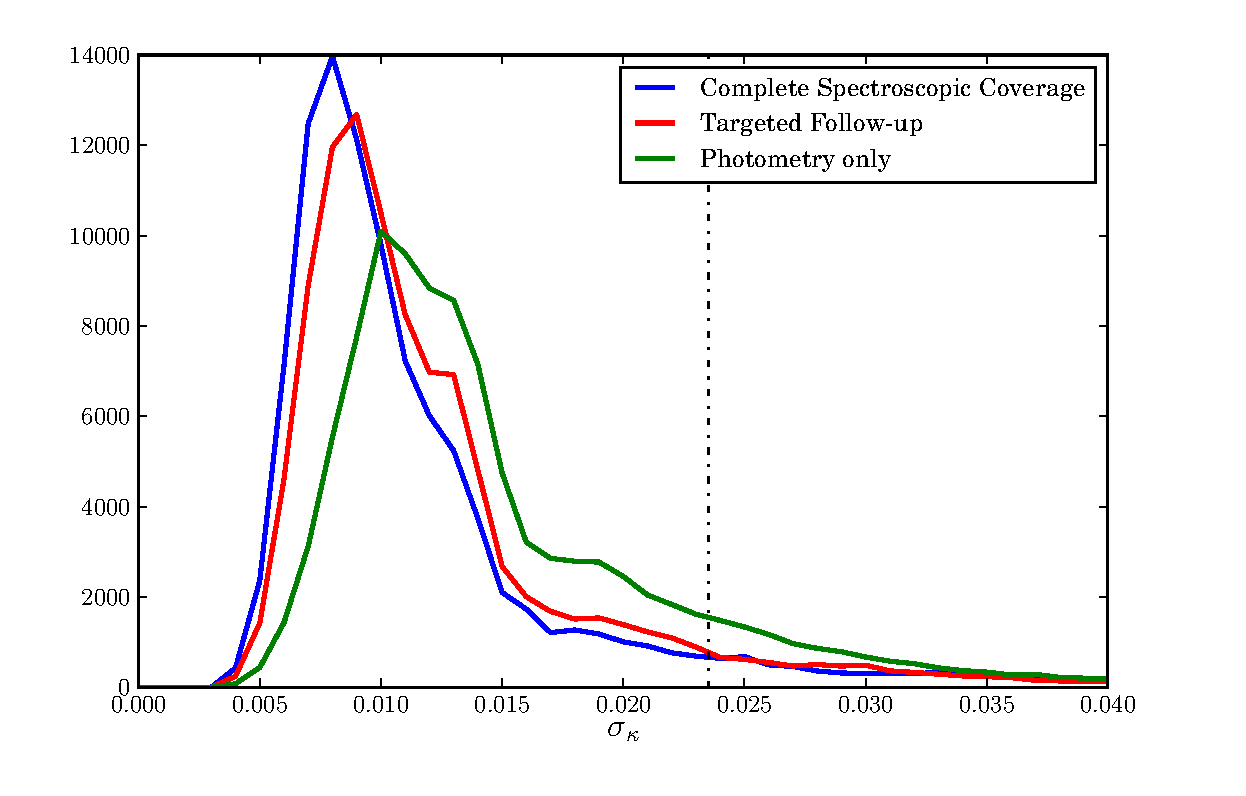
\includegraphics[width=\columnwidth]{figs/Width.eps}
\caption{The widths of the \infered PDFs $\pr(\kappax|\data)$ for
$10^5$ lines of sight, given different quality of data. 
Blue: spectroscopic redshift for every halo with $i<26$; 
Red: spectroscopic redshift for every halo with $i<23$, 
and every halo with $i<24$ within 1 arcminute, while all other objects just
have photometric redshifts;
Green: all the objects in the field have only photometric redshifts. The
vertical dot-dashed line marks the width of the global $\pr(\kappax)$ for all
lines of sight.}
\label{fig:reconwidths}
\end{figure}
%%%%%%%%%%%%%%%%%%%%%%%%%

%%%%%%%%%%%%%%%%%%%%%%%%%
\begin{figure}
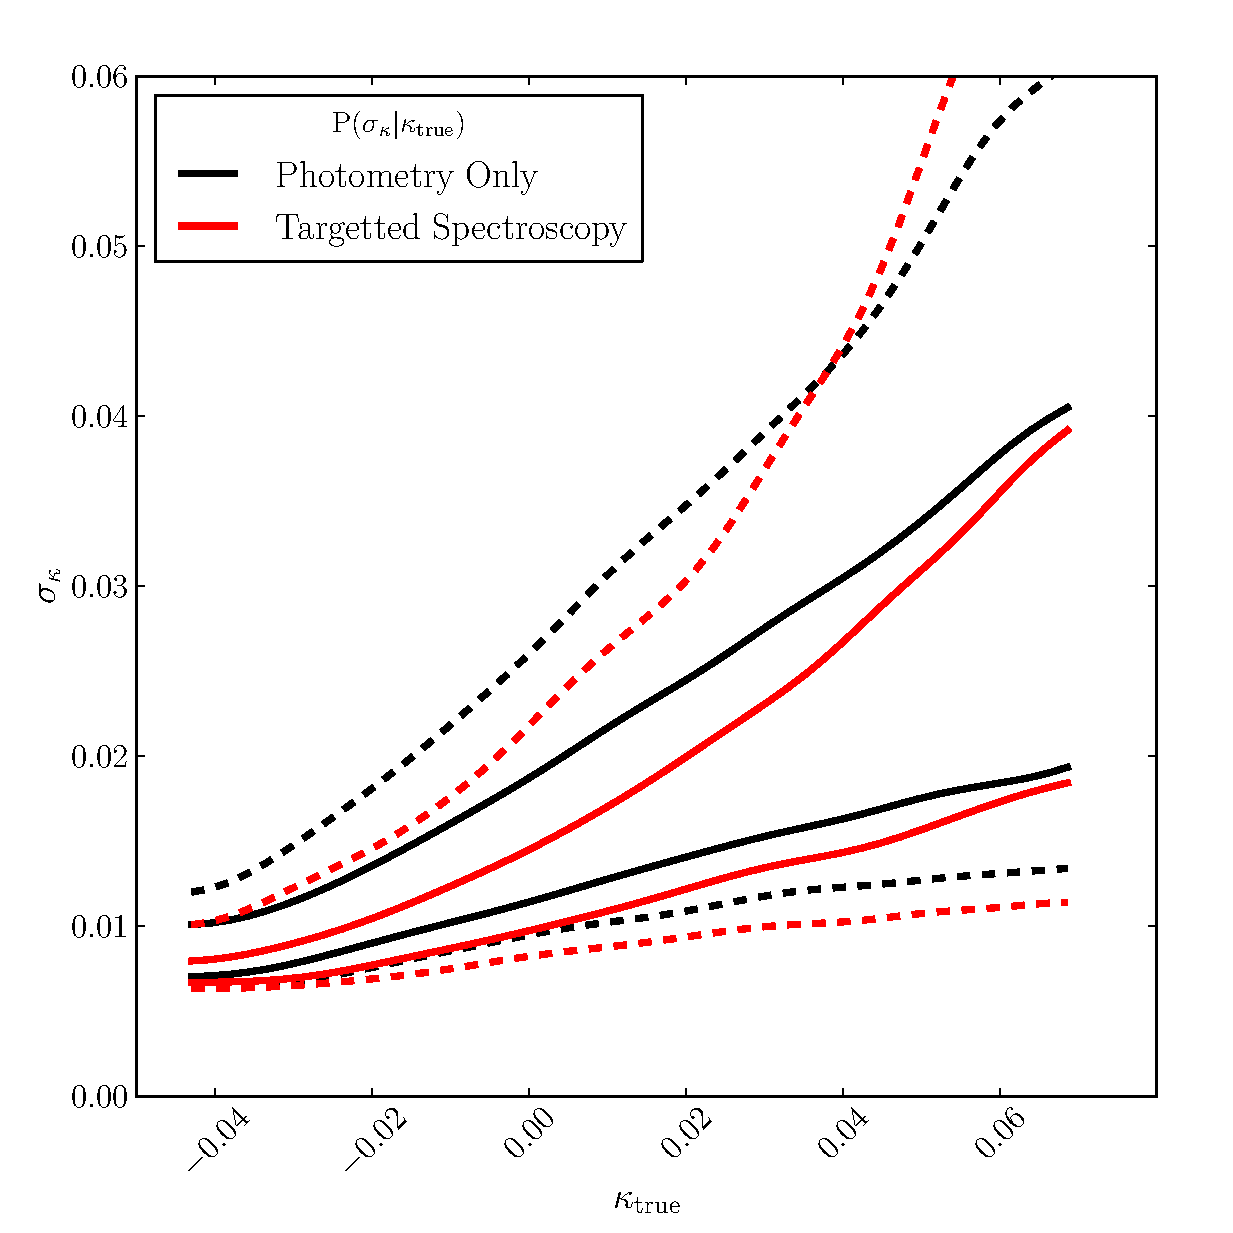
\includegraphics[width=\columnwidth]{figs/WidthvsHilbert.eps}
\caption{Width of the \infered PDF $\pr(\kappax|\data)$ as a function of 
the true convergence, $\kappaxtrue$, for two different data qualities. 
Black assumes only photometric redshifts for all objects,
while red assumes a campaign of targeted spectroscopy. The region between the
solid (dashed) lines contains 68\% (95\%) of lines-of-sight.}
\label{fig:widthsvsH}
\end{figure}
%%%%%%%%%%%%%%%%%%%%%%%%%

The best possible reconstructions of $\kappax$ will come from having a
spectroscopic redshift for every single object in each field.
\Fref{fig:reconwidths} shows the distribution of $\kappax$ posterior 
PDF widths for various data qualities: complete spectroscopic coverage results
in the smallest widths. In terms of telescope time, such a reconstruction
would likely be prohibitively expensive, but we investigate this scenario as
an ideal case. 

\comment{PJM: The following does not belong here because \Fref{fig:widthsvsH}
does not show results for spectroscopic redshifts only!}

Reconstructing the lines of sight with perfect knowledge of the
redshift but an uncertain stellar mass, we find that the width of
$\pr(\kappax|\data)$ grows with the expectation of $\kappax$ and the ray-traced $\kappatrue$
(\Fref{fig:widthsvsH}). The low $\kappax$ lines of sight are relatively empty,
and so there are few opportunities for uncertainties in the halo masses to
\propogate into $\kappax$ uncertainties; low $\kappax$ lines of sight can be reconstructed
more precisely than high $\kappax$ lines of sight.


% % % % % % % % % % % % % % % % % % % % % % % % % % % % % % % % % % % % % % % 

\subsection{Reconstructing $\kappax$ from photometry alone}

Inferring the stellar mass of a galaxy from its magnitude and colours requires
an estimate of how far away the galaxy is; without a spectroscopic redshift
the \infered stellar mass is less precise. However, obtaining photometry has
much lower observational cost; all upcoming large area photometric surveys
will reach 24th magnitude, providing sufficient data to reconstruct lines of
sight  {\it without} additional observations. In principle the photometric
redshift is correlated with the \infered stellar mass, however we do not model
this effect since the convergence from the outskirts of an individual halo is
only weakly \dependant on redshift at fixed mass due to the breadth of the
lensing kernel: the redshift uncertainty has only a small effect on the
inferred $\pr(\kappax|\data)$ in comparison to that of  the uncertain stellar
masses.  With only photometric redshifts, the uncertainty on $\kappah$ is
larger than in the spectroscopic case, and this \propogates into a broader
$\pr(\kappax|\data)$, as can be seen in \Fref{fig:reconwidths}. However, the
photometric reconstruction still typically produces a 50\% improvement
compared to the precision of the global $\pr(\kappax)$. 

\tom{With photometric data alone, $\kappah^{\rm med}$ can shift by $\sim$0.01
relative to $\kappah^{\rm med}$ given spectroscopic coverage. Since  the
$\kappax$ contribution of voids cannot change with data quality, the shift in
$\kappah^{\rm med}$ must be due to the asymmetric propagation of stellar mass
uncertainties into $\kappax$ uncertainties. As the stellar mass uncertainty
increases, $\kappah^{\rm med}$ is pushed higher.  To correctly calibrate 
$\pr(\kappax|\kappah^{\rm med},\data)$ one {\it must} include the data quality
used to generate $\kappah^{\rm med}$.}

We find that the width of $\pr(\kappax|\data)$ grows with the expectation
value of $\kappax$; this is shown in \Fref{fig:widthsvsH}. The low $\kappax$
lines of sight are relatively empty, and so there are few opportunities for
uncertainties in the halo masses to \propogate into $\kappax$ uncertainties.

%\flag{Is there a simple approximation for $\kappax$ and $\sigma_{\kappa}$ as a
%function of $\kappaxtrue$? This would be useful when making forecasts, writing
%proposals etc...}
%
%TEC: No. It's also not relevant to proposals since kappatrue isnt observable. One can ask is there
%a formula for sigmakappa given the expectation value of kappax. The answer to that is
%yes, but it depends on data quality. Concerning forecasting yes we would 
%want to use a simple approximation, but I don't think it has a place in this paper.
%When you/I/someone does the forecasting I'd like to be involved; I'll make the
%approximation then.


% % % % % % % % % % % % % % % % % % % % % % % % % % % % % % % % % % % % % % % 

\subsection{Reconstructing $\kappax$ with partial spectroscopic coverage}
\label{sec:obsMstar+z:targetedspec}

While a fully photometric reconstruction provides useful constraints on
$\pr(\kappax|\data)$, targeted spectroscopy can provide additional constraints
on the masses and redshifts of halos whose $\kappah$ contributions have the
largest absolute uncertainty. Obtaining spectra of bright ($i<22$) objects is
relatively fast with large telescopes: however, we find that if spectroscopic
redshifts were known for all $i<22$ galaxies in our fields the reconstruction
improves only slightly over the purely photometric reconstruction,  although
the improvement can depend strongly on the details of the particular line of
sight. Obtaining spectra for fainter objects would be correspondingly more
expensive, but if spectroscopic redshifts could be obtained for all $i<23$
galaxies (as part of a futuristic baryon acoustic oscillation survey, for
example) and all $i<24$ galaxies within 1 arcminute of the line of sight, then
we find that the $\pr(\kappax|\data)$ would be almost as precise as that from
having complete spectroscopic coverage (\Fref{fig:reconwidths}). If any object is
extremely close to the lines of sight our approximation of weakly lensing
mass-sheets will break down; also, neglecting baryonic effects will also be a poor
approximation; a spectrum will be needed
to adequately model systems with very well alligned pertrubers.
Consistent with our previous findings, the lowest $\kappax$ lines of
sight have the most constrained $\kappax$ PDFs.


%%%%%%%%%%%%%%%%%%%%%%%%%%%%%%%%%%%%%%%%%%%%%%%%%%%%%%%%%%%%%%%%%%%%%%%%%%%%%%

\section{Systematic Errors due to Sample Selection}
\label{sec:biases}


\begin{figure*}
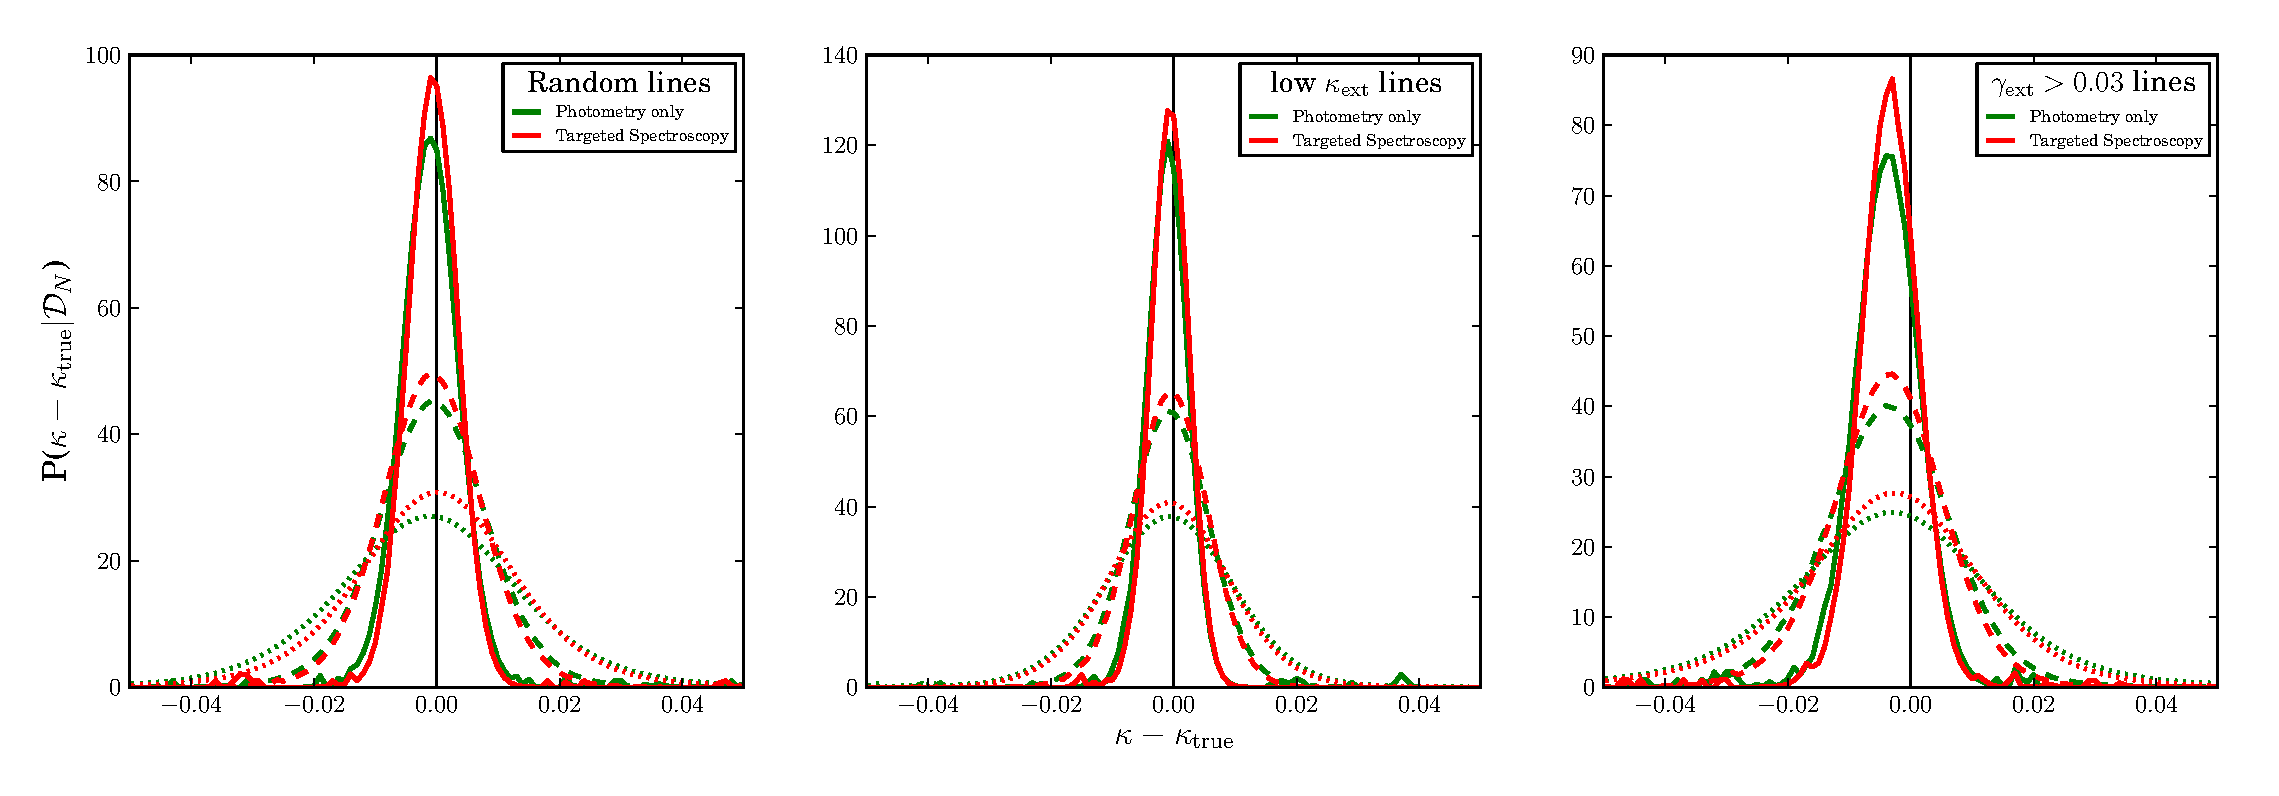
\includegraphics[width=\textwidth]{figs/biasplots.eps}
\caption{Accuracy in $\kappax$ from combining samples of lenses.  These plots
show the expectation value of $\prod_{i=1}^N \pr_i(\kappax-\kappaxtrue|\data)$ --
deviations from zero represent biases. The solid, dashed and dotted lines
correspond to combinations of  20, 5 and 2 sightlines respectively. Black
lines show the results \infered from photometry alone, whilst red lines show
the results  from the same targeted spectroscopy campaign described in 
\Sref{sec:obsMstar+z:targetedspec}. The three panels correspond to samples of
sightlines selected in different ways. Left: randomly selected lines of
sight.  Centre: sightlines randomly selected from the 33\% of lines whose
P($\kappax$) is most tightly constrained by our model.  Right: lines of sight
with external shear of 0.05 or greater.}
\label{fig:biasplots}
\end{figure*}

While it is good to reconstruct $\kappax$ precisely, it is more important that
$\kappax$ is reconstructed accurately. The reconstruction must not be biased. 
We quantify the accuracy of our reconstructed $\pr(\kappax|\data)$ in the
following way. By shifting the \infered $\pr(\kappax|\data)$ for each line of
sight by the true (ray-traced) convergence, we obtain a  PDF that should be
centred on zero; these offset PDFs can be multiplied together for multiple
lines of sight to emulate a joint likelihood analysis, and then test for
possible bias in it:
\be
\label{eq:bias}
\mathcal{P}_N = \prod_{i=1}^N \pr_i(\kappax-\kappax^{\rm true}|\data)
\ee
In this section, we quantify the bias as the size of the deviation in the
expectation value of $\mathcal{P}_N$ from zero. If the bias of $\mathcal{P}_N$
is smaller than the half-width of $\mathcal{P}_N$, our $\kappax$ inferences
can be considered accurate. Since the width of $\mathcal{P}_N$ decreases as
more sightlines are combined, a small bias will always 
eventually be found. In the context of measuring time-delay distance at the 
one percent level, the expectation value of $|\mathcal{P}_N|$ needs to be 
significantly less than 0.01. \tom{External convergence is not the only source
of uncertainty in measuring time-delay distance. Since the statistical
distance uncertainties due to lens modelling and time delay estimation are
likely to be at the 3-4\% level \citep{SuyuEtal2010}, convolving
$\mathcal{P}_N$ with a Gaussian of width $0.04/\sqrt{N}$ is a reasonable
approximation for the likely final uncertainty on time-delay distance.}


% \comment{From Sherry:
% Re: $P_N$:
% Not sure that this is the best way to quantify bias.  First of all, this
% doesn't include the modeling error of $\sim3-4\%$, so the number of lenses listed
% (for when <$P_N$> = half width of $P_N$) is underestimated.  Also, with this
% definition, a large number of lenses could be described as "biased" even if
% the resulting shift is say 0.0001, which won't really trouble us at all.  For
% example, what would the distributions look like in Fig.8 with 100 lenses? 
% Since the peaks of the red curves are within 0.01 of kappa_true, I would
% suspect that with a large number of lenses, the corresponding red curve would
% be within 0.01 of kappa_true.  The present day goal is to get H0 to 1\%, and
% it would be good to state somewhere that with targeted spectroscopy, one could
% recover kext at the 1\% level with a large sample of lenses.}

The source of systematic error that we investigate in this paper  is that of
sample selection: we define three different example selections of lines of
sight, and compute the bias  \phil{that would result (if left unaccounted
for)} in each one in turn, as a function of data quality. The results
described below are illustrated in \Fref{fig:biasplots}.


% % % % % % % % % % % % % % % % % % % % % % % % % % % % % % % % % % % % % % % 

\subsection{Selecting random lines of sight}
\label{sec:bias:random}

We first consider a purely random selection of lines of sight. With the purely
photometric reconstruction, there is no evidence of bias, even after combining
20 lines of sight. \tom{This result is a sanity check: if we had chosen lines
of sight with identical $\kappah^{\rm med}$ rather than $\kappah^{\rm
med}\pm0.003$, randomly selected lines of sight would have zero bias by
construction}. If lines of sight hosting time delay lenses are truely random, 
our method allows $\kappax$ to be reconstructed without inducing a bias (under
the basic assumptions that the universe is like the calibration simulation,
and the correct stellar-mass to halo-mass relation has been used). 


% % % % % % % % % % % % % % % % % % % % % % % % % % % % % % % % % % % % % % % 

\subsection{Selecting only the lines of sight with narrow $\pr(\kappax|\data)$}
\label{sec:bias:tightPDF}

Since follow-up campaigns (such as high resolution imaging, or time
variability monitoring) are expensive, it is likely that only a subset of
detected objects will be observed further. By pre-selecting objects that have 
the best-constrained convergence, the cosmological value per lens can be
increased. However, this selection \phil{(like any other)}
has the potential to induce a bias. It is
likely that only photometry will be available at the time of sub-sample
selection (although spectroscopic follow-up might be conducted at a later
date). We mimic such a selection by drawing lines of sight only from those in
the lowest third of $\sigma_{\kappa}$, given a purely photometric
reconstruction of their fields. 

We find that selecting the most tightly constrained lines of sight in this way
does not introduce a significant bias:  our reconstruction is most accurate
for the lowest $\kappax$ lines of sight. Combining 20 such systems, the bias
is at the 0.001 level.

Photometry of the field seems to be sufficient to adequately select these
empty lines of sight.  However, 
since lenses are typically massive galaxies and hence found in locally over-dense
environments, it is unlikely that  an almost empty line of sight would
actually  contain a lens; \phil{what we can say is that if the local
environment can be identified spectroscopically, and then the line
of sight mass distribution reconstructed using our method, selecting lenses
with low, well-constrained values of $\kappax$ will lead to an increase in
distance precision at no cost in bias.}

% % % % % % % % % % % % % % % % % % % % % % % % % % % % % % % % % % % % % % % 

\subsection{Selecting only high shear lines of sight}
\label{sec:bias:tightPDF}

Time delay lenses are often selected for follow-up based on their images'
brightness (to make monitoring observations less expensive), their images'
separation (to decrease the covariance between the ground-based image
light-curves), or the fact that they are quadruply-imaging rather than
doubly-imaging (since this yields 3 time delays instead of 1, a higher
magnification and a more informative Einstein Ring system). All three of these
properties favour lenses with high convergence and shear along their lines of
sight. Focusing on the quad selection, we might expect many of these systems
to have significant external shear (since the cross-section for 4 image
production is so sensitive to ellipticity in the lens mass distribution (or
equivalently, external shear due to the lens' environment). 

\phil{We can test the impact of such a shear selection by selecting only lines
of sight with an external shear above some threshold.  We define a somewhat
extreme selection  of $\gammax>0.05$, and find that in this sample, $\kappax$
would be systematically underestimated at the $\sim$0.008 level (corresponding
to a 0.8\% systematic error in distance).}  In the absence of other sources of
uncertainty, this systematic error would be significant in a sample of just 5
lenses; when including other time-delay distance uncertainties a 0.8\% bias would be
significant for $\sim$20 lenses. This systematic error is mitigated if only the lines of sight with both
$\gammax>0.05$ and well constrained $\pr(\kappax|\data)$ are used, but in this
case a bias at the $\sim$0.005 level remains. 

While $\gammax>0.05$ is likely to be a much stronger selection than would
occur in reality, it is  nevertheless worth noting from this example that the
reconstruction \proceedure \phil{can be biased if lens selection functions are
extreme and unaccounted for.} Since our model does not include shear
constraints it is not surprising that a selection function based on shear can
induce a bias. A more sophisticated model that includes the shear recovered
from the lens modelling might be less susceptible to this bias.

The halo model can also be used to estimate the external shear along a line of
sight: shear is an observable that can be extracted from strong lens
modelling. However, there is a degeneracy between internal and external shear.
When the Einstein Ring imaging data are very good it is possible to
disentangle external and internal shear \citep[\eg][]{SuyuEtal2010}, but there
are still significant uncertainties. \citet{WongEtal2011} attempted to match
the shear from strong lens models with a reconstruction of the local lens
group environment, but found a tension between the strong lens model and the
reconstruction of the environment. Given the \citet{WongEtal2011} results, it
is unclear whether the external shear from lens models can be reconciled with
a line-of-sight reconstruction. Alternatively, it may be possible  to infer
external shear using weak lensing information from near the line of sight.  If
the true external shear can be measured, it provides an additional constraint
on which of the \MS lines of sight are similar to the reconstructed line of
sight. \citet{SuyuEtal2012} found that in the case of 
RXJ1131-1231, combining shear constraints
with galaxy number count over-density gave a significantly different
$\pr(\kappax|\gamma,N_{45})$ compared to the PDF from number count
over-density alone, $\pr(\kappax|N_{45})$.

Extending our model to include shear we find that given
perfect knowledge of the halo mass and redshift the ray-traced external shear
$\gamma$ and the reconstructed external shear $\gamma_{\mathrm{h}}$  are
similar, with 68 percent of lines obeying
\be
\label{eq:shearineq}
|{\pmb{\gamma}_{\mathrm{ext}}-\pmb{\gamma}_{\mathrm{h}}}| < \mathrm{0.025}
\ee 
Future work should investigate whether $\gamma_{\mathrm{h}}$ can be used
to improve the accuracy and precision of $\kappax$ estimation, given a
reconstruction of the line of sight. 

%%%%%%%%%%%%%%%%%%%%%%%%%%%%%%%%%%%%%%%%%%%%%%%%%%%%%%%%%%%%%%%%%%%%%%%%%%%%%%

\section{Systematic Errors due to using an incorrect Stellar Mass--Halo Mass Relation}
\label{sec:SHAMfail}

\begin{figure*}
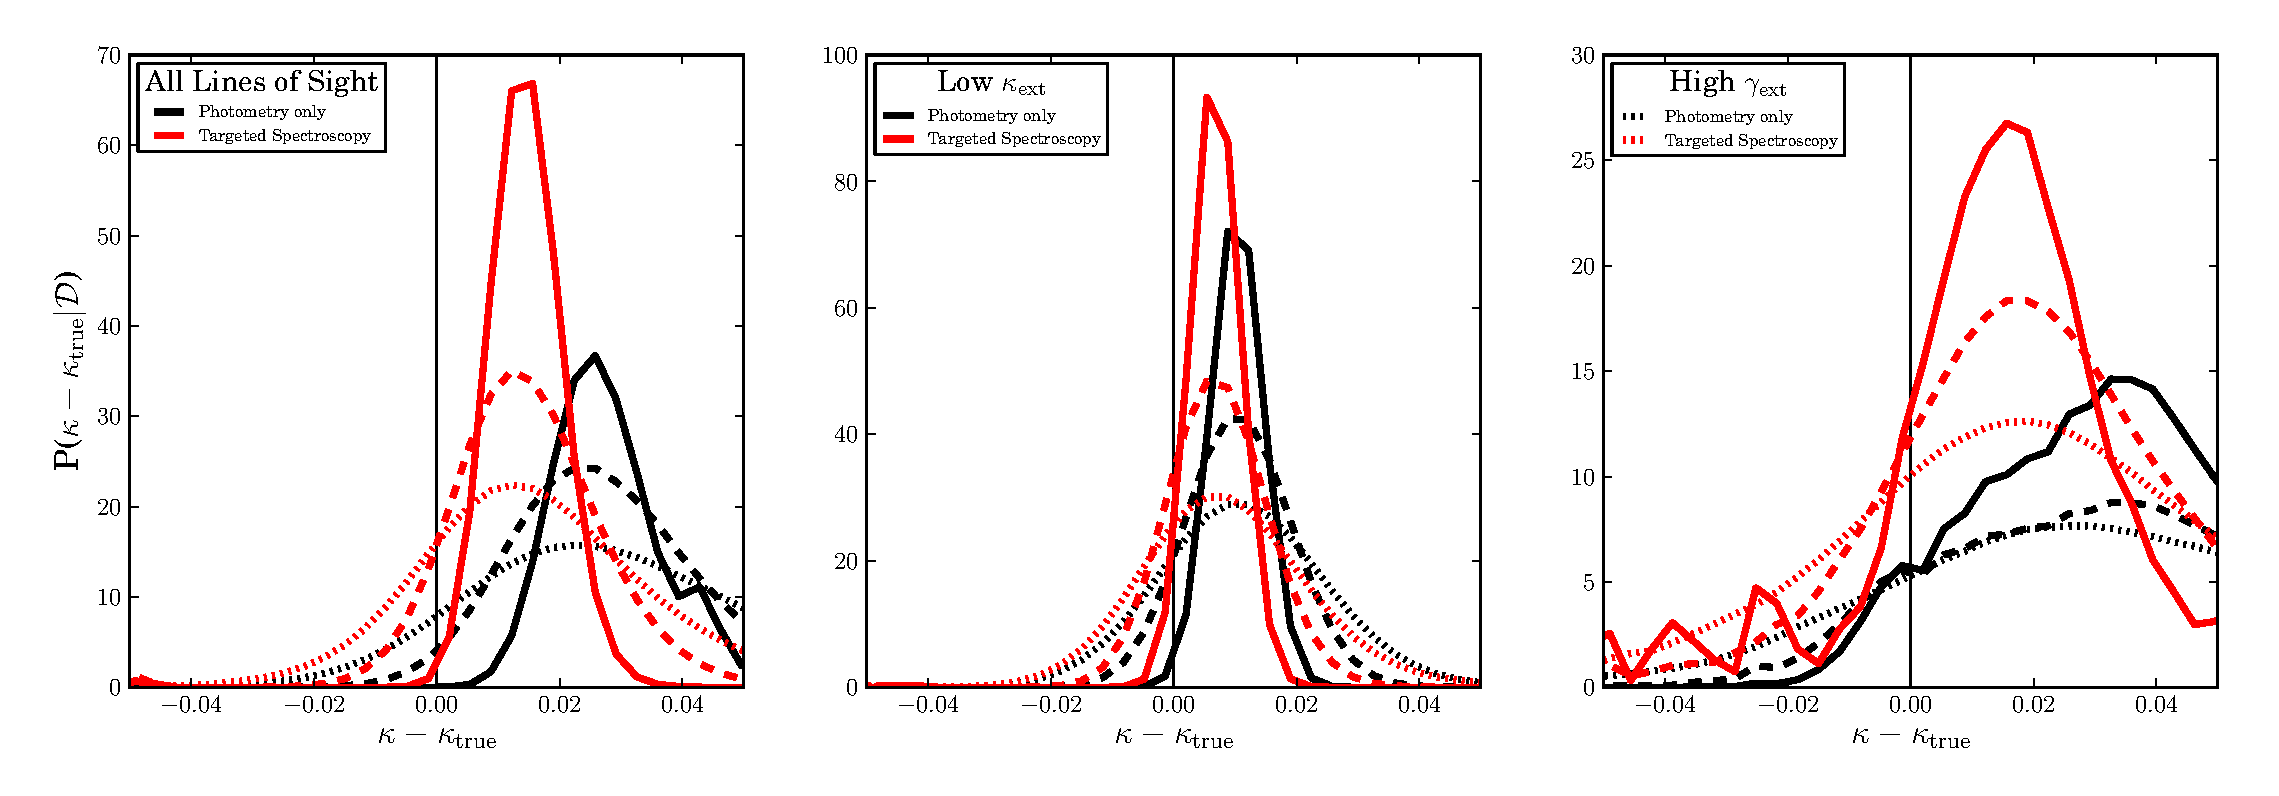
\includegraphics[width=\textwidth]{figs/SHAMbias.eps}
\caption{Systematic bias in $\kappax$ due to reconstructing lines of sight with the wrong stellar mass--halo mass relation. The real stellar masses were created using the relation of \citet{MosterEtal2010}, but the reconstruction and calibration assumes the relation of \citet{BehrooziEtal2010}.  These plots
show the expectation value of $\prod_{i=1}^N \pr_i(\kappax-\kappaxtrue|\data)$ --
deviations from zero represent biases. The solid, dashed and dotted lines
correspond to combinations of  20, 5 and 2 sightlines respectively. Black
lines show the results \infered from photometry alone, whilst red lines show
the results  from the same targeted spectroscopy campaign described in 
\Sref{sec:obsMstar+z:targetedspec}. The three panels correspond to samples of
sightlines selected in different ways. Left: randomly selected lines of
sight.  Centre: sightlines randomly selected from the 33\% of lines whose
P($\kappax$) is most tightly constrained by our model.  Right: lines of sight
with external shear of 0.05 or greater.}
\label{fig:SHAMbias}
\end{figure*}

\new{
Throughout this work we have assumed that the universe's halos are populated with galaxies whose stellar masses are determined purely by the \citet{BehrooziEtal2010} Stellar Mass--Halo Mass relation. The real universe is unlikely to follow this relation perfectly; the result is that an ensemble of real lines of sight will differ from the ensemble of calibration lines of sight, potentially introducing a systematic error to the reconstructed convergence.

It is hard to test the size of this sytematic error, since we do not know how much the real universe differs from the chosen Stellar Mass--Halo Mass relation. As wider and deeper surveys are conducted more data will become available with which to construct the Stellar Mass--Halo Mass relation; this should drive the infered Stellar Mass--Halo Mass relation closer to the truth. We are only interested in testing the effect of changing the Stellar Mass--Halo Mass relation in a way that is consistant with observational constraints; improving the observational contraints on the Stellar Mass--Halo Mass relation will decrease the the size of the systematic error on reconstructed $\kappax$ induced by assuming a specfic Stellar Mass--Halo Mass relation.

To estimate the potential size of this systematic error we use the Behroozi relation to generate the stellar masses of our calibration lines of sight, but the stellar mass--halo mass relation of Moster for the ``real'' lines of sight that are reconstructed. For halos masses of $\sim 10^{12} \Msun$ both stellar mass--halo mass relations estimate a stellar mass of $\sim 10^{10.5} \Msun$, but for halos more massive that this the stellar masses generated from the Moster relation are systematically higher than those generated from the Behroozi relation. At halo masses of $\sim 10^{14} \Msun$ the best fit stellar masses differ by $\sim 0.25$ dex. 

Applying our Behroozi--based reconstruction to lines of sight with Moster stellar masses results in systematically overestimating $\kappax$. In \Fref{fig:SHAMbias} we show the resulting bias on the inferred $\kappax$ after combining several lines of sight. With a purely photometric reconstruction there is a typical systematic bias of $\sim 0.025$ on the reconstructed convergence, although it can be shrunk to $\sim 0.01$ if only the low $\kappax$ lines of sight are used, however for the high shear lines of sight the bias is $\sim 0.04$. It is not suprising that the low $\kappax$ lines of sight are least affected by changes in the stellar mass--halo mass relation. Low $\kappax$ lines of sight are relatively empty hence their $\kappah$ values are small and do not change significantly with stellar mass--halo mass relation. The high shear lines of sight have significantly overestimated $\kappax$ since they tend to lie close to massive halos. This is the regime where the Moster and Behroozi relations are most different. Interestingly overestimating the $\kappah$ values of high shear lines of sight pushes them into the region where the $\kappah$ to $\kappax$ calibration is least certain; this has significantly decreased the precision of the reconstructed $\kappax$. 

Despite the systematic errors the photometric reconstruction is still sufficient to choose the best lines of sight for spectroscopic follow-up. With targetted spectroscopy the systematic error decreases to $\sim 0.014$ for the ensemble, $\sim 0.005$ for the low kappa sample and $\sim 0.018$ for the high shear sample. This result provides further motivation for prioritizing the lenses that reside on the underdense lines of sight.

The systematic errors reported herein may be overly pessimistic; the bias is due to differences in the stellar masses predicted for high mass halos. If observations can discriminate between the high mass end of the Behroozi and Moster relations then the systematic error on the reconstruction will decrease.
}

%%%%%%%%%%%%%%%%%%%%%%%%%%%%%%%%%%%%%%%%%%%%%%%%%%%%%%%%%%%%%%%%%%%%%%%%%
%\section{Improving precision by including additional information}
%\notes{placeholder for shear}
%%%%%%%%%%%%%%%%%%%%%%%%%%%%%%%%%%%%%%%%%%%%%%%%%%%%%%%%%%%%%%%%%%%%%%%%%

\section{Discussion}
\label{sec:discuss}

% \comments{
% We have shown that reconstructing the matter due to halos along any line of
% sight can improve the constraints on the external convergence along that line
% of sight, with, depending on sample selection,  the width of
% $\pr(\kappax|\data)$ being up to a factor of two smaller than the global
% $\pr(\kappax)$, and  we have quantified the residual bias in the $\kappax$
% estimates under our calibration assumptions. We now revisit these assumptions.
% }

The total convergence along a line of sight is strongly correlated with the
reconstructed $\kappah$. However, since our model ignores voids and assumes
all halos follow a spherical truncated-NFW profile our halo model does not
include all of the relevant physics; hence, the width of our resulting
$\pr(\kappax|\data)$ is still typically $\sim$0.01 for any given lightcone,
even assuming perfect knowledge of every halo's virial mass and redshift. To
make further progress a more advanced treatment of both voids and halos will
be needed. \citet{KarpenkaEtal2012} find that their supernova data prefer, in
the context of their simple halo model, a truncated isothermal profile for the
galaxy mass distributions. Galaxy-galaxy and cluster-galaxy  lensing studies
\citep[\eg][]{GavazziEtal2007,JohnstonEtal2007, LagattutaEtal2010} also suggest an approximately
isothermal profile for the mass-shear correlation function; however, at large
radii these profiles are dominated by the effects of neighbouring halos, which
are already taken into account by our model.  Further iterations on the
analysis presented here should include the stellar mass distributions that
cause the isothermal density profiles in the centres of galaxies, although we
do not expect this to have a big impact on the reconstructions. Likewise, 
halo ellipticity
may have some small effect on the predicted convergence. It
is possible that baryonic physics may alter the radial profile of dark
matter halos, even on large scales. \citet{Semboloni+2012} found that baryonic
physics had a 30-40\% impact on three-point shear statistics, it is unclear
how baryons affect one-point convergence statistics compared to the pure dark
matter simulations used in this work.

Clusters, filaments and voids are more difficult to model, but simple forms
could in principle be derived from the structures found in the simulations,
and included in the halo model in some way.  Most importantly for the highest
$\kappax$ lines of sight will be a better group and cluster model:
\citet{MomchevaEtal2006} and  \citet{WongEtal2011} recommend using models
where dark mass is assigned to both galaxy-scale halos and halos for the
groups and clusters they occupy. To make this work, one could incorporate a
group and cluster finder, and then infer halo mass from optical richness
\citep[\eg][]{MaxBCG} in tandem with BCG stellar mass. \new{A group finder would also
allow us to identify central and satellites galaxies; in this work we have neglected
the differences between central halos and satellites. However, given perfect knowledge of halo masses
we found that only in 5 percent of sightlines do satellites
contribute over 20 percent of the sightline's total $\kappax$. Introducing a group finder
is unlikely to provide major improvement to the reconstruction of satellites.}
\tom{Meanwhile,
improving the modelling of voids could be done using suggestions by
\citet{voids2} or \citet{voids1} combined with a void finder such as in
\citet{voids3}. Combining an advanced halo model with a void model will allow
a direct test of the halo approximation: using real photometric data one could
reconstruct lines of sight and compare against measured weak lensing shears.
This would ensure that the reconstruction model reproduces the contents of the
real universe, rather than a particular simulation.}

% \comments{Interestingly, we have found that it is the most empty lines of sight that 
% can be reconstructed with the highest precision. $\kappax$ estimates for empty
% lines of sight receive few contributions from halos, and a large contribution
% from voids; since they have the tightest PDFs after the reconstruction it
% seems that our model's biggest uncertainties are driven by naively
% reconstructing halos rather than neglecting voids. With a photometric
% reconstruction of the field there is a significant broadening, but the
% resulting precision is still typically 50\%  higher than using the global
% $\kappax$ distribution.
% 
% Since the uncertainty on $\pr(\kappax|\data)$ is $\sim$0.01 even
% with perfect knowledge of halo mass and redshift, it seems that modelling uncertainties
% from voids, deviations from sphericity and dark matter clumping within the
% main halo dominate the total $\kappax$ uncertainty even with very
% uncertain stellar masses. Inferring halo ellipticity and dark matter
% clumping will likely always remain a difficulty for line of sight
% reconstruction; but as \Fref{fig:magcut} shows, observing deeper
% than 24th magnitude does not significantly help the reconstruction.
% }

% \comments{For a small fraction of lines of sight, $\pr(\kappax|\data)$ remains very
% broad even after applying our reconstruction; these lines of sight are
% typically the most over-dense lines of sight in the universe. For
% time-delay cosmography the most observationally expensive tasks are the
% light-curve monitoring and high resolution follow-up imaging and spectroscopy,
% while making photometric observations of a
% 4$\times$4 arcminute patch of sky survey down to 24th magnitude is
% relatively cheap. We have shown that with a single epoch observation of
% the region around a strong lens it is possible to infer $\pr(\kappax|\data)$.
% If a line of sight has a broad $\pr(\kappax|\data)$ it can be rejected {\it
% before} the investment of follow-up. We find that
% selecting only the lines of sight with the most tightly constrained
% $\pr(\kappax)$ does not induce a bias in $\kappax$, and hence distance.
% For the most over-dense lines of sight,
% the precision of $\pr(\kappax|\data)$ is improved noticeably by the addition
% of spectroscopic information; currently insufficient time-delay systems are
% know to choose a subset based on their reconstructed $\pr(\kappax|\data)$.
% Spectroscopic coverage will definitely be useful for extracting cosmology from
% over-dense lines of sight.
% }
% %%%%%%%%%%%%%%%%%%%%%%%%%%%%%%
% \comments{%
% \begin{figure}
% 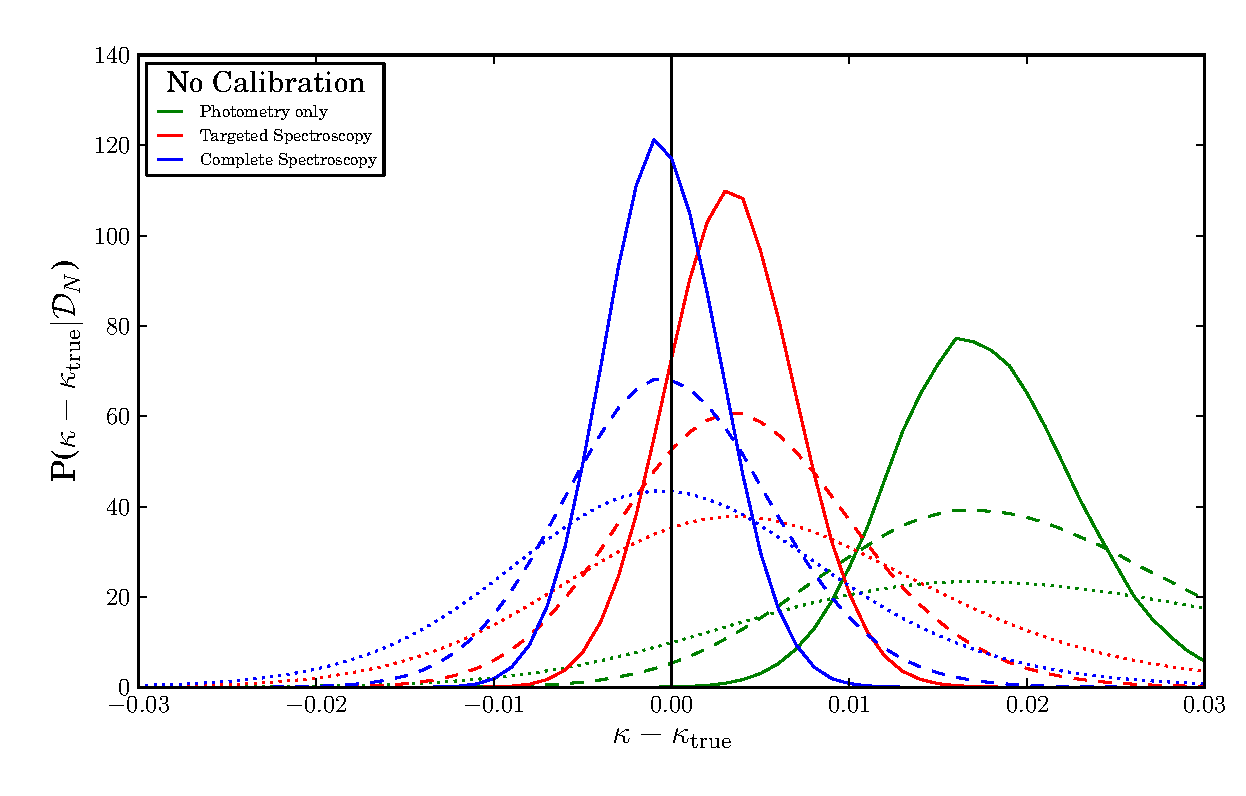
\includegraphics[width=\columnwidth]{figs/biasplots3.eps}
% \caption{Convergence estimation accuracy using the full  $\pr(\kappax|\kappah)$
% distribution, rather than its median.  As in \Fref{fig:biasplots}, solid,
% dashed and dotted lines show combinations of 20, 5 and 2 lines of sight
% respectively, while green lines show the inferences 
% from photometry alone, red lines from photometry and targeted spectroscopy 
% (assuming a spectroscopic redshift for all
% halos with $i<23$ and all halos within 1 arcminute and $i<24$), and blue lines
% from the unrealistic assumption of a spectroscopic redshift for all galaxies
% in the field. }
% \label{fig:no-median-tricks}
% \end{figure}
% }%
%%%%%%%%%%%%%%%%%%%%%%%%%%%%%%

The reduction of $\pr(\kappah|\data)$ to just its median value, before using
it to look up the appropriate $\pr(\kappax)$ from the simulated sightline
ensemble, is reminiscent of the procedure followed by \citet{SuyuEtal2010},
and Greene et al (submitted). The reconstruction method presented here can be
seen as the limiting case of the weightings explored by Greene et al: rather
than using weighted number counts in an aperture, we treat each galaxy
individually, and predict $\kappa_{\rm h,obs}^{\rm med}$ for use in their
place. Given photometry alone, our reconstruction represents a $\sim$50\% improvement of
the precision compared the number counts used in \citet{SuyuEtal2010}. Greene et al.
made important progress for the most over-dense lines of sight; our
reconstructions are $\sim$30\% more precise than those of Greene et al.
The use of relative overdensities by Suyu et al. and Greene et al. may decrease 
their sensitivity to the choice of calibration simulation; this work's use of
absolute convergence may be less robust to changes in the calibration simulation. 


% \comments{ One
% significant disadvantage of these types of method is that they impose a
% bottleneck in the flow of information. Once you have compressed to one number,
% it is difficult to incorporate more information later; you have to recompute
% all the calibrations. Using the full PDF for $\kappah$ is the more correct
% thing to do: at present, however, it suffers from significant bias in the
% photometric data case. \Fref{fig:no-median-tricks} shows how $\kappax$ is
% overestimated, as a result of the high scatter in halo mass for objects with 
% high stellar mass. As has already been noted, 
% future work should focus on increasing the precision of the halo
% mass estimates. 
% }

In this work, we have used  the \MS as a calibration tool. If the real
Universe is not like the \MS, then this calibration will be incorrect.
Repeating this study using a different simulation to make the test catalogues
would allow us to quantify the sensitivity of our results to the simulation
used. Similarly the use of a different semi-analytic model to paint galaxies
onto halos would enable similar exploration of these systematic errors. 
\citet{SuyuEtal2010}
used the relative over-density to mitigate the effect of simulatioan and
simulation, but it does not completely remove the dependence on simulation.
\new{We have tested the effect of using a different stellar mass--halo mass relation
and found that this can induce significant systematic biases if the true relation is unknown.} Future work should include
investigating the robustness of the reconstruction to these systematic errors \new{and develope proscriptions that mitigate against them}

% \comments{In particular, the method presented here is tied to the simulations at two
% points: the prior PDF for $\kappah$, and the conditional distribution
% $\pr(\kappax|\kappah)$ used to convert halo model convergence to total
% convergence. The first tie could potentially be avoided if the halo mass
% estimation gave rise to a reasonable $\pr(\kappah|\data)$ on its own.
% Possibilities for improving the precision of the halo mass estimation are
% discussed above. The second tie is more difficult, since breaking it means
% modelling the unseen mass structures and voids. It
% should be possible to infer hierarchically  the parameters of a flexible model
% for these things from the data itself, as demonstrated by
% \citet{KarpenkaEtal2012} (albeit under the assumption of scatter-free scaling
% relations) -- how this affects the cosmographic precision is to be
% investigated. When working with wide field imaging surveys,  weak lensing shears will be
% available around every line of sight:  fitting these with the halo models
% described here in order to constrain the hyper-parameters of the model presents a 
% possible test of our halo model prescription against real observations.
% }
%%%%%%%%%%%%%%%%%%%%%%%%%%%%%%%%%%%%%%%%%%%%%%%%%%%%%%%%%%%%%%%%%%%%%%%%%

\section{Conclusions}
\label{sec:conclude}

In this work we have investigated a simple halo model prescription for
reconstructing all the mass along a line of sight to an intermediate redshift
source. We have used the ray-traced lensing convergence along lines of sight
through the Millennium Simulation to calibrate estimates of the total
convergence made by summing the convergences due to each object in a
photometric catalogue. Having found that the reconstruction process is
accurate given this calibration and perfect knowledge of halo mass and
redshift, we investigated the effects of reasonable uncertainties in the
stellar mass and redshift of each halo, and propagated these uncertainties
into a $\pr(\kappax|\data)$ for each line of sight. We also defined three
different possible line of sight selections, and investigated the possible 
bias induced by these selections. We draw the following conclusions:

\begin{itemize} 

\item Despite our model's simplicity, its reconstructed $\kappah$ values are
good tracers of $\kappax$. $\kappah$ is biased due to our ignorance of voids,
groups and clusters, and the unseen mass in small halos and filaments, but we
find that this can be calibrated out using the Millenium Simulation
catalogues. We found that with perfect knowledge of every halo's mass and
redshift,  calibrated reconstruction of a typical line of sight  gives an
unbiased estimate of $\kappax$ that is not perfect, but is $1.8$ 
times more precise than the global
$\pr(\kappax)$. This factor quantifies the limit to which the halo model can
represent the external convergence due to line of sight mass structure.

\item With uncertain halo masses and redshifts, we find that
$\pr(\kappah|\data)$ can still be calibrated in order to infer
$\pr(\kappax|\data)$ from the ensemble of simulated lines of sight, but the
resulting PDFs tend to be much broader than for perfect halo mass and redshift
reconstructions.

\item It is very rare for halos further than 2 arcminutes from the line of
sight to make a significant contribution to $\pr(\kappax|\data)$; likewise, 
including
halos whose host galaxy is less luminous than $i=24$ does not significantly
improve our reconstructions.  A photometric survey to this depth of a
4$\times$4 arcminute patch around the target would approach the limiting
uncertainties of our simple reconstruction recipe, and yield a 
$\pr(\kappax|\data)$ that has, on average, a width of 0.016 (inducing a $\sim$1.6\%
uncertainty on time-delay distances). This is 1.5 times
less broad than the global $\pr(\kappax)$. 

\item  For the most over-dense lines of sight, the reconstruction produces a
broad PDF; conversely, we find that the lines of sight with the sharpest
inferred $\pr(\kappax|\data)$ are typically under-dense. Since the
reconstructions described here can be performed before follow-up time is
invested, it will be possible to select targets by the precision of their
$\kappax$ estimates. This will be useful in an era when there are more known
lenses than can be followed-up. Photometric data are sufficient to select the best lines of sight for
follow-up. Spectroscopic coverage helps to tighten  $\pr(\kappax|\data)$ for
most lines of sight.
% , but is of less use for low $\kappax$ lines of
% sight.

\item Selecting from the highest precision 33\% of the reconstructed lines of
sight results in a sample with low bias, $\sim$0.1\% in terms of the
time-delay distance. \tom{For these lines of sight the reconstructed
$\pr(\kappax|\data)$ induces a statistical uncertainty of $\sim$1\% on
individual time-delay distances.}

\item Conversely, selecting lines of sight with high shear ($|\gamma| > 0.05$; 
a somewhat extreme selection, but one that  could potentially arise from 
focusing on four-image or wide separation lenses) results in a sample with
bias of 0.8\% in time delay distance (and hence $H_0$). Including realistic estimates of other
sources of uncertainty a systematic error of 0.8\% would become significant in
a sample of $\sim$20 lenses. The addition of shear constraints to our model might
alleviate this potential systematic.

\item \new{Reconstructing a line of sight with an incorrect stellar mass--halo mass relation can introduce systematic errors on the inferrred time-delay distance at the percent level. This error can only be reduced by tightening the observational limits on the stellar mass--halo mass relation at the high mass end.}

% \item With only a photometric reconstruction of all time delay lens fields,
% and following up only the systems with the most precise $\kappax$ estimates,
% the width of the dominant statistical uncertainty in time-delay cosmography
% can be halved, without inducing biases at the one percent level.

\end{itemize}

% PJM: Im not sure this is the right note to end on. 

% TEC: I liked it! but it's open to discussion.


% External convergence is not the only uncertainty in time delay cosmology, but
% for systems like B1608$+$656 it is the dominant one. For most lines of sight
% lens modelling induces uncertainties at the $\sim$4 percent
% level, which far exceeds the typical $\kappax$ uncertainties after applying our
% reconstruction \proceedure. By using reconstruction methods such as that
% explored here to select the most appropriate 
% lenses for follow-up, the uncertainties due to line of sight
% convergence will become a sub-dominant source of error.

While we have tested our reconstruction method against realistic simulations
of line of sight mass distributions in the Universe, our method is also 
calibrated to these simulations. Testing this assumption in the short term,
and replacing it with an empirical calibration (or hierarchical inference) in
the longer term, are worthy goals for future work. The halo model framework is
flexible enough to enable many such improvements, including, quite naturally,
the incorporation of more information from observations. 


%%%%%%%%%%%%%%%%%%%%%%%%%%%%%%%%%%%%%%%%%%%%%%%%%%%%%%%%%%%%%%%%%%%%%%%%
%%  ACKNOWLEDGMENTS
%%%%%%%%%%%%%%%%%%%%%%%%%%%%%%%%%%%%%%%%%%%%%%%%%%%%%%%%%%%%%%%%%%%%%%%%

\section*{Acknowledgements}
 
TEC thanks Vasily Belokurov for supervision, guidance and suggestions.
We thank Risa Wechsler and Peter Behroozi 
for useful discussions and suggestions. We are grateful to the referee
for suggesting improvements to the original manuscript.
\input{acknowledgments.tex}

%%%%%%%%%%%%%%%%%%%%%%%%%%%%%%%%%%%%%%%%%%%%%%%%%%%%%%%%%%%%%%%%%%%%%%%%%%%%%%
%  APPENDICES
%%%%%%%%%%%%%%%%%%%%%%%%%%%%%%%%%%%%%%%%%%%%%%%%%%%%%%%%%%%%%%%%%%%%%%%%%%%%%%

\appendix

%%%%%%%%%%%%%%%%%%%%%%%%%%%%%%%%%%%%%%%%%%%%%%%%%%%%%%%%%%%%%%%%%%%%%%%%%%%%%%

\section{Inferring $\Mhalo$ given a noisy measurement of $\Mstarobs$}
\label{appendix:MSMH}

To estimate the convergence caused by a halo we need to know its mass; how can 
halo mass be \infered from a noisy estimate of the stellar mass $\Mstarobs$
of a galaxy at redshift $z$. We seek the posterior
PDF $\Pr(\Mhalo|\Mstarobs,z)$, which can be expanded as follows:

\begin{eqnarray}
&& \Pr(\Mhalo|\Mstarobs,z) = \notag\\
&& \int d\Mstar \Pr(\Mhalo|\Mstar,z) \Pr(\Mstar|\Mstarobs,z), \notag\\
&\propto& \int d\Mstar \Pr(\Mstarobs|\Mstar) \Pr(\Mstar|\Mhalo,z) \Pr(\Mhalo|z),
\label{eq:mhalo-mstar}
\end{eqnarray}
where we have used Bayes' Theorem twice to replace
$\Pr(\Mhalo|\Mstar,z) \Pr(\Mstar|z)$ with 
$\Pr(\Mstar|\Mhalo,z) \Pr(\Mhalo|z)$, and 
to invert $\Pr(\Mstar|\Mstarobs)$ into the sampling
distribution $\Pr(\Mstar|\Mstarobs)$, which we recognise as the likelihood
function for the observed stellar mass. Note that the ``true'' $\Mstar$ of the
galaxy is marginalised out: we are only interested in inferring the halo
mass. The last two terms in
\eqref{eq:mhalo-mstar} are the $\Mstar-\Mhalo$ relation from
\citet{BehrooziEtal2010}, and the halo mass function $\Pr(\Mhalo|z)$, at the
given redshift. We can
tabulate the product of these two from our Millennium Simulation catalogue,
constructing a two-dimensional histogram of halo masses and their associated
true stellar masses (drawn from the Behroozi relation). 

For each galaxy, we compute the likelihood function for its $\Mstarobs$ as a
function of the unknown $\Mstar$, and multiply it by our tabulated joint PDF.
This heavily downweights halos with $\Mstar$ values outside the observed
range. We then do the marginalisation integral by Monte Carlo, drawing
(two-dimensional) sample parameter vectors
from the down weighted histogram, discarding the $\Mstar$ values, and
constructing a one-dimensional histogram that is an estimate of
$\Pr(\Mhalo|\Mstarobs)$.

If the redshift of the galaxy is uncertain, we need to take this
uncertainty into account; for example, for each sample drawn from the
photometric redshift posterior PDF $\Pr(z|{\rm colors})$, we can draw a
sample $\Mhalo$ using the above procedure.

%%%%%%%%%%%%%%%%%%%%%%%%%%%%%%%%%%%%%%%%%%%%%%%%%%%%%%%%%%%%%%%%%%%%%%%%%%%%%%
%  REFERENCES
%%%%%%%%%%%%%%%%%%%%%%%%%%%%%%%%%%%%%%%%%%%%%%%%%%%%%%%%%%%%%%%%%%%%%%%%%%%%%%

% MNRAS does not use bibtex, input .bbl file instead. 
% Generate this in the makefile using bubble script in scriptutils:

% bubble -f paper-lcr.tex references.bib 
% \input{paper-lcr.bbl}

% \bibliographystyle{apj}
% \bibliography{references}

\input{references.tex}

%%%%%%%%%%%%%%%%%%%%%%%%%%%%%%%%%%%%%%%%%%%%%%%%%%%%%%%%%%%%%%%%%%%%%%%%%%%%%%

\label{lastpage}
\bsp

\end{document}

%%%%%%%%%%%%%%%%%%%%%%%%%%%%%%%%%%%%%%%%%%%%%%%%%%%%%%%%%%%%%%%%%%%%%%%%%%%%%%


% \bibliographystyle{apj}
% \bibliography{references}

\begin{thebibliography}{99}


\bibitem[{{Auger} {et~al.}(2007){Auger}, {Fassnacht}, {Abrahamse}, {Lubin}, \&
  {Squires}}]{AugerEtal2007}
{Auger}, M.~W., {Fassnacht}, C.~D., {Abrahamse}, A.~L., {Lubin}, L.~M., \&
  {Squires}, G.~K. 2007, \aj, 134, 668

\bibitem[Auger(2008)]{Auger2008} Auger, M.~W.\ 2008, \mnras, 383, 
L40 

\bibitem[\protect\citeauthoryear{Auger et al.}{2009}]{AugerEtal2009} 
Auger M.~W., Treu T., Bolton A.~S., Gavazzi R., Koopmans L.~V.~E., Marshall 
P.~J., Bundy K., Moustakas L.~A., 2009, ApJ, 705, 1099 


\bibitem[\protect\citeauthoryear{Auger et al.}{2010}]{AugerEtal2010} 
Auger M.~W., Treu T., Bolton A.~S., Gavazzi R., Koopmans L.~V.~E., Marshall 
P.~J., Moustakas L.~A., Burles S., 2010, ApJ, 724, 511 


\bibitem[\protect\citeauthoryear{Baltz, Marshall, 
\& Oguri}{2009}]{BMO} Baltz E.~A., Marshall P., Oguri M., 2009, JCAP, 1, 15 


\bibitem[\protect\citeauthoryear{Behroozi, Conroy, 
\& Wechsler}{2010}]{BehrooziEtal2010} Behroozi P.~S., Conroy C., Wechsler R.~H., 2010, ApJ, 717, 379 


\bibitem[\protect\citeauthoryear{Ben{\'{\i}}tez}{2000}]{BPZ} Ben{\'{\i}}tez N., 2000, ApJ, 536, 571 


\bibitem[{{Brada{\v c}} {et~al.}(2009){Brada{\v c}}, {Treu}, {Applegate},
  {Gonzalez}, {Clowe}, {Forman}, {Jones}, {Marshall}, {Schneider}, \&
  {Zaritsky}}]{BradacEtal2009}
{Brada{\v c}}, M., {et~al.} 2009, \apj, 706, 1201

\bibitem[Cropper et al.(2012)]{Euclid} Cropper, M., Cole, R., 
James, A., et al.\ 2012, arXiv:1208.3369 


\bibitem[\protect\citeauthoryear{Collett et 
al.}{2012}]{CollettEtal2012a} Collett T.~E., Auger M.~W., Belokurov V., 
Marshall P.~J., Hall A.~C., 2012, MNRAS, 424, 2864 


% \bibitem[Dalal(2005)]{Dalal2005} Dalal, N.\ 2005, 25 Years After 
% the Discovery: Some Current Topics on Lensed QSOs,  


\bibitem[{{Dalal} {et~al.}(2005){Dalal}, {Hennawi}, \& {Bode}}]{DalalEtal2005}
{Dalal}, N., {Hennawi}, J.~F., \& {Bode}, P. 2005, \apj, 622, 99


\bibitem[\protect\citeauthoryear{De Lucia 
\& Blaizot}{2007}]{DeLucia+Blaizot2007} De Lucia G., Blaizot J., 2007, MNRAS, 375, 2 


\bibitem[Fadely et al.(2010)]{FadelyEtal2009} Fadely, R., Keeton, 
C.~R., Nakajima, R., \& Bernstein, G.~M.\ 2010, \apj, 711, 246 


\bibitem[\protect\citeauthoryear{Falco, Gorenstein, 
\& Shapiro}{1985}]{FalcoEtal1985} Falco E.~E., Gorenstein M.~V., Shapiro I.~I., 1985, ApJ, 289, L1 


\bibitem[{{Fassnacht} \& {Lubin}(2002)}]{Fassnacht+Lubin2002}
{Fassnacht}, C.~D., \& {Lubin}, L.~M. 2002, \aj, 123, 627

\bibitem[Fassnacht et al.(2006)]{FassnachtEtal2006} Fassnacht, C.~D., 
Gal, R.~R., Lubin, L.~M., et al.\ 2006, \apj, 642, 30 

\bibitem[\protect\citeauthoryear{Fassnacht, Koopmans, 
\& Wong}{2011}]{FassnachtEtal2011} Fassnacht C.~D., Koopmans L.~V.~E., Wong K.~C., 2011, MNRAS, 410, 2167 

\bibitem[Foster 
\& Nelson(2009)]{voids3} Foster, C., \& Nelson, L.~A.\ 2009, \apj, 699, 1252 

\bibitem[Gavazzi et al.(2007)]{GavazziEtal2007} Gavazzi, R., Treu, T., 
Rhodes, J.~D., et al.\ 2007, \apj, 667, 176 

\bibitem[\protect\citeauthoryear{Gavazzi et 
al.}{2008}]{GavazziEtal2008} Gavazzi R., Treu T., Koopmans L.~V.~E., 
Bolton A.~S., Moustakas L.~A., Burles S., Marshall P.~J., 2008, ApJ, 677, 
1046 

\bibitem[Gunnarsson et al.(2006)]{GunnarssonEtal2006} Gunnarsson, C., 
Dahl{\'e}n, T., Goobar, A., J{\"o}nsson, J., M{\"o}rtsell, E.\ 2006, \apj, 640, 417 

\bibitem[Higuchi et al.(2012)]{voids1} Higuchi, Y., Oguri, M., 
\& Hamana, T.\ 2012, arXiv:1211.5966 

\bibitem[{{Hilbert} {et~al.}(2007){Hilbert}, {White}, {Hartlap}, \&
  {Schneider}}]{HilbertEtal2007}
{Hilbert}, S., {White}, S.~D.~M., {Hartlap}, J., \& {Schneider}, P. 2007,
  \mnras, 382, 121

\bibitem[\protect\citeauthoryear{Hilbert et 
al.}{2009}]{HilbertEtal2009} Hilbert S., Hartlap J., White S.~D.~M., Schneider P., 2009, A\&A, 499, 31 

\bibitem[Hilbert et al.(2011)]{HilbertEtal2011} Hilbert, S., Gair, 
J.~R., \& King, L.~J.\ 2011, \mnras, 412, 1023 

\bibitem[Holder 
\& Schechter(2003)]{Holder+Schechter2003} Holder, G.~P., \& Schechter, P.~L.\ 2003, \apj, 589, 688 


\bibitem[\protect\citeauthoryear{Holz 
\& Wald}{1998}]{Holz+Wald1998} Holz D.~E., Wald R.~M., 1998, PhRvD, 58, 063501 

\bibitem[Holz 
\& Linder(2005)]{Holz+Linder2005} Holz, D.~E., \& Linder, E.~V.\ 2005, \apj, 631, 678 

\bibitem[J{\"o}nsson et al.(2010)]{JonssonEtal2010} J{\"o}nsson, J., 
Dahl{\'e}n, T., Hook, I., Goobar, A., M{\"o}rtsell, E.\ 2010, \mnras, 402, 526 

\bibitem[Johnston et al.(2007)]{JohnstonEtal2007} Johnston, D.~E., 
Sheldon, E.~S., Wechsler, R.~H., et al.\ 2007, arXiv:0709.1159 


\bibitem[Karpenka et al.(2012)]{KarpenkaEtal2012} Karpenka, N.~V., 
March, M.~C., Feroz, F., \& Hobson, M.~P.\ 2012, arXiv:1207.3708 

\bibitem[Kauffmann et al.(1999)]{KauffmannEtal1999} Kauffmann, G., 
Colberg, J.~M., Diaferio, A., \& White, S.~D.~M.\ 1999, \mnras, 303, 188
\bibitem[Krause et al.(2012)]{voids2} Krause, E., Chang, 
T.-C., Dor{\'e}, O., \& Umetsu, K.\ 2012, arXiv:1210.2446 

\bibitem[{{Keeton} \& {Zabludoff}(2004)}]{Keeton+Zabludoff2004}
{Keeton}, C.~R., \& {Zabludoff}, A.~I. 2004, \apj, 612, 660

\bibitem[\protect\citeauthoryear{Keeton 
\& Moustakas}{2009}]{Keeton+Moustakas2009} Keeton C.~R., Moustakas L.~A., 2009, ApJ, 699, 1720 

% \bibitem[\protect\citeauthoryear{Linder 
% \& Holz}{2004}]{Linder+Holz2004} Linder E.~V., Holz D.~E., 2004, AAS, 36, \#131.02 

\bibitem[Koester et al.(2007)]{MaxBCG} Koester, B.~P., McKay, 
T.~A., Annis, J., et al.\ 2007, \apj, 660, 221 

\bibitem[Koopmans et al.(2003)]{KoopmansEtal2003} Koopmans, L.~V.~E., 
Treu, T., Fassnacht, C.~D., Blandford, R.~D., 
\& Surpi, G.\ 2003, \apj, 599, 70 


\bibitem[Koopmans(2004)]{Koopmans2004} Koopmans, L.~V.~E.\ 2004, 
arXiv:astro-ph/0412596 

\bibitem[Lagattuta et al.(2010)]{LagattutaEtal2010} Lagattuta, D.~J., 
Fassnacht, C.~D., Auger, M.~W., et al.\ 2010, \apj, 716, 1579 

\bibitem[LSST Science Collaboration (2009)]{LSST} LSST 
Science Collaboration: Abell, P.~A., Allison, J., et al.\ 2009, 
arXiv:0912.0201 

\bibitem[Macci{\`o} et al.(2008)]{MaccioEtal2008} Macci{\`o}, A.~V., 
Dutton, A.~A., \& van den Bosch, F.~C.\ 2008, \mnras, 391, 1940 

\bibitem[Mandelbaum et al.(2009)]{Mandelbaum} Mandelbaum, R., van 
de Ven, G., \& Keeton, C.~R.\ 2009, \mnras, 398, 635 



\bibitem[{{Momcheva} {et~al.}(2006){Momcheva}, {Williams}, {Keeton}, \&
  {Zabludoff}}]{MomchevaEtal2006}
{Momcheva}, I., {Williams}, K., {Keeton}, C., \& {Zabludoff}, A. 2006, \apj,
  641, 169

\bibitem[Nakajima et al.(2009)]{NakajimaEtal2009} Nakajima, R., 
Bernstein, G.~M., Fadely, R., Keeton, C.~R., 
\& Schrabback, T.\ 2009, \apj, 697, 1793 

\bibitem[\protect\citeauthoryear{Navarro, Frenk, 
\& White}{1997}]{NFW} Navarro J.~F., Frenk C.~S., White S.~D.~M., 1997, ApJ, 490, 493 


\bibitem[\protect\citeauthoryear{Neto et al.}{2007}]{Neto2007} 
Neto A.~F., et al., 2007, MNRAS, 381, 1450 


\bibitem[{{Oguri} \& {Takahashi}(2006)}]{Oguri+Takahashi2006}
{Oguri}, M., \& {Takahashi}, K. 2006, \prd, 73, 123002

\bibitem[\protect\citeauthoryear{Oguri 
\& Marshall}{2010}]{Oguri+Marshall2010} Oguri M., Marshall P.~J., 2010, MNRAS, 405, 2579 


\bibitem[\protect\citeauthoryear{Oke}{1974}]{Oke1974} Oke 
J.~B., 1974, ApJS, 27, 21 

\bibitem[Schneider(2006)]{Schneider2006} Schneider, P.\ 2006, 
in Saas-Fee Advanced Course 33: Gravitational Lensing: Strong, Weak and Micro, 
269 

\bibitem[Semboloni et al.(2012)]{Semboloni+2012} Semboloni, E., 
Hoekstra, H., \& Schaye, J.\ 2012, arXiv:1210.7303 


\bibitem[\protect\citeauthoryear{Springel et 
al.}{2005}]{SpringelEtal2005} Springel V., et al., 2005, Natur, 435, 629 


\bibitem[\protect\citeauthoryear{Suyu}{2012}]{Suyu2012a} Suyu 
S.~H., 2012, arXiv, arXiv:1202.0287 


\bibitem[\protect\citeauthoryear{Suyu et al.}{2012}]{SuyuEtal2012} 
Suyu S.~H., et al., 2012, arXiv, arXiv:1208.6010 


\bibitem[\protect\citeauthoryear{Suyu et al.}{2010}]{SuyuEtal2010} 
Suyu S.~H., Marshall P.~J., Auger M.~W., Hilbert S., Blandford R.~D., 
Koopmans L.~V.~E., Fassnacht C.~D., Treu T., 2010, ApJ, 711, 201 

\bibitem[Takahashi et al.(2011)]{TakahashiEtal2011} Takahashi, R., Oguri, 
M., Sato, M., \& Hamana, T.\ 2011, \apj, 742, 15 


\bibitem[Treu et al.(2009)]{TreuEtal2009} Treu, T., Gavazzi, R., 
Gorecki, A., et al.\ 2009, \apj, 690, 670 

\bibitem[\protect\citeauthoryear{Vale 
\& White}{2003}]{Vale+White2003} Vale C., White M., 2003, ApJ, 592, 699 

\bibitem[Wambsganss et al.(2004)]{WambsganssEtal2004} Wambsganss, J., 
Bode, P., \& Ostriker, J.~P.\ 2004, \apjl, 606, L93 

\bibitem[{{Wang} \& {Dai}(2011)}]{Wang+Dai2011}
{Wang}, F.~Y., \& {Dai}, Z.~G. 2011, \aap, 536, A96


\bibitem[{{Williams} {et~al.}(2006){Williams}, {Momcheva}, {Keeton},
  {Zabludoff}, \& {Leh{\'a}r}}]{WilliamsEtal2006}
{Williams}, K.~A., {Momcheva}, I., {Keeton}, C.~R., {Zabludoff}, A.~I., \&
  {Leh{\'a}r}, J. 2006, \apj, 646, 85


\bibitem[\protect\citeauthoryear{Wong et al.}{2011}]{WongEtal2011} 
Wong K.~C., Keeton C.~R., Williams K.~A., Momcheva I.~G., Zabludoff A.~I., 
2011, ApJ, 726, 84 


\bibitem[{{Wong} {et~al.}(2012){Wong}, {Ammons}, {Keeton}, \&
  {Zabludoff}}]{WongEtal2012}
{Wong}, K.~C., {Ammons}, S.~M., {Keeton}, C.~R., \& {Zabludoff}, A.~I. 2012,
  \apj, 752, 104

\bibitem[\protect\citeauthoryear{Wyithe et al.}{2011}]{WyitheEtal2011} Wyithe, J.~S.~B., Yan, 
H., Windhorst, R.~A., \& Mao, S.\ 2011, \nat, 469, 181 


% \bibitem[\protect\citeauthoryear{\tom{which paper}}{{9999}}]{xxx} 
% None

\end{thebibliography}


%%%%%%%%%%%%%%%%%%%%%%%%%%%%%%%%%%%%%%%%%%%%%%%%%%%%%%%%%%%%%%%%%%%%%%%%%%%%%%

\label{lastpage}
\bsp

\end{document}

%%%%%%%%%%%%%%%%%%%%%%%%%%%%%%%%%%%%%%%%%%%%%%%%%%%%%%%%%%%%%%%%%%%%%%%%%%%%%%


% \bibliographystyle{apj}
% \bibliography{references}

\begin{thebibliography}{99}


\bibitem[{{Auger} {et~al.}(2007){Auger}, {Fassnacht}, {Abrahamse}, {Lubin}, \&
  {Squires}}]{AugerEtal2007}
{Auger}, M.~W., {Fassnacht}, C.~D., {Abrahamse}, A.~L., {Lubin}, L.~M., \&
  {Squires}, G.~K. 2007, \aj, 134, 668

\bibitem[Auger(2008)]{Auger2008} Auger, M.~W.\ 2008, \mnras, 383, 
L40 

\bibitem[\protect\citeauthoryear{Auger et al.}{2009}]{AugerEtal2009} 
Auger M.~W., Treu T., Bolton A.~S., Gavazzi R., Koopmans L.~V.~E., Marshall 
P.~J., Bundy K., Moustakas L.~A., 2009, ApJ, 705, 1099 


\bibitem[\protect\citeauthoryear{Auger et al.}{2010}]{AugerEtal2010} 
Auger M.~W., Treu T., Bolton A.~S., Gavazzi R., Koopmans L.~V.~E., Marshall 
P.~J., Moustakas L.~A., Burles S., 2010, ApJ, 724, 511 


\bibitem[\protect\citeauthoryear{Baltz, Marshall, 
\& Oguri}{2009}]{BMO} Baltz E.~A., Marshall P., Oguri M., 2009, JCAP, 1, 15 


\bibitem[\protect\citeauthoryear{Behroozi, Conroy, 
\& Wechsler}{2010}]{BehrooziEtal2010} Behroozi P.~S., Conroy C., Wechsler R.~H., 2010, ApJ, 717, 379 


\bibitem[\protect\citeauthoryear{Ben{\'{\i}}tez}{2000}]{BPZ} Ben{\'{\i}}tez N., 2000, ApJ, 536, 571 


\bibitem[{{Brada{\v c}} {et~al.}(2009){Brada{\v c}}, {Treu}, {Applegate},
  {Gonzalez}, {Clowe}, {Forman}, {Jones}, {Marshall}, {Schneider}, \&
  {Zaritsky}}]{BradacEtal2009}
{Brada{\v c}}, M., {et~al.} 2009, \apj, 706, 1201

\bibitem[Cropper et al.(2012)]{Euclid} Cropper, M., Cole, R., 
James, A., et al.\ 2012, arXiv:1208.3369 


\bibitem[\protect\citeauthoryear{Collett et 
al.}{2012}]{CollettEtal2012a} Collett T.~E., Auger M.~W., Belokurov V., 
Marshall P.~J., Hall A.~C., 2012, MNRAS, 424, 2864 


% \bibitem[Dalal(2005)]{Dalal2005} Dalal, N.\ 2005, 25 Years After 
% the Discovery: Some Current Topics on Lensed QSOs,  


\bibitem[{{Dalal} {et~al.}(2005){Dalal}, {Hennawi}, \& {Bode}}]{DalalEtal2005}
{Dalal}, N., {Hennawi}, J.~F., \& {Bode}, P. 2005, \apj, 622, 99


\bibitem[\protect\citeauthoryear{De Lucia 
\& Blaizot}{2007}]{DeLucia+Blaizot2007} De Lucia G., Blaizot J., 2007, MNRAS, 375, 2 


\bibitem[Fadely et al.(2010)]{FadelyEtal2009} Fadely, R., Keeton, 
C.~R., Nakajima, R., \& Bernstein, G.~M.\ 2010, \apj, 711, 246 


\bibitem[\protect\citeauthoryear{Falco, Gorenstein, 
\& Shapiro}{1985}]{FalcoEtal1985} Falco E.~E., Gorenstein M.~V., Shapiro I.~I., 1985, ApJ, 289, L1 


\bibitem[{{Fassnacht} \& {Lubin}(2002)}]{Fassnacht+Lubin2002}
{Fassnacht}, C.~D., \& {Lubin}, L.~M. 2002, \aj, 123, 627

\bibitem[Fassnacht et al.(2006)]{FassnachtEtal2006} Fassnacht, C.~D., 
Gal, R.~R., Lubin, L.~M., et al.\ 2006, \apj, 642, 30 

\bibitem[\protect\citeauthoryear{Fassnacht, Koopmans, 
\& Wong}{2011}]{FassnachtEtal2011} Fassnacht C.~D., Koopmans L.~V.~E., Wong K.~C., 2011, MNRAS, 410, 2167 

\bibitem[Foster 
\& Nelson(2009)]{voids3} Foster, C., \& Nelson, L.~A.\ 2009, \apj, 699, 1252 

\bibitem[Gavazzi et al.(2007)]{GavazziEtal2007} Gavazzi, R., Treu, T., 
Rhodes, J.~D., et al.\ 2007, \apj, 667, 176 

\bibitem[\protect\citeauthoryear{Gavazzi et 
al.}{2008}]{GavazziEtal2008} Gavazzi R., Treu T., Koopmans L.~V.~E., 
Bolton A.~S., Moustakas L.~A., Burles S., Marshall P.~J., 2008, ApJ, 677, 
1046 

\bibitem[Gunnarsson et al.(2006)]{GunnarssonEtal2006} Gunnarsson, C., 
Dahl{\'e}n, T., Goobar, A., J{\"o}nsson, J., M{\"o}rtsell, E.\ 2006, \apj, 640, 417 

\bibitem[Higuchi et al.(2012)]{voids1} Higuchi, Y., Oguri, M., 
\& Hamana, T.\ 2012, arXiv:1211.5966 

\bibitem[{{Hilbert} {et~al.}(2007){Hilbert}, {White}, {Hartlap}, \&
  {Schneider}}]{HilbertEtal2007}
{Hilbert}, S., {White}, S.~D.~M., {Hartlap}, J., \& {Schneider}, P. 2007,
  \mnras, 382, 121

\bibitem[\protect\citeauthoryear{Hilbert et 
al.}{2009}]{HilbertEtal2009} Hilbert S., Hartlap J., White S.~D.~M., Schneider P., 2009, A\&A, 499, 31 

\bibitem[Hilbert et al.(2011)]{HilbertEtal2011} Hilbert, S., Gair, 
J.~R., \& King, L.~J.\ 2011, \mnras, 412, 1023 

\bibitem[Holder 
\& Schechter(2003)]{Holder+Schechter2003} Holder, G.~P., \& Schechter, P.~L.\ 2003, \apj, 589, 688 


\bibitem[\protect\citeauthoryear{Holz 
\& Wald}{1998}]{Holz+Wald1998} Holz D.~E., Wald R.~M., 1998, PhRvD, 58, 063501 

\bibitem[Holz 
\& Linder(2005)]{Holz+Linder2005} Holz, D.~E., \& Linder, E.~V.\ 2005, \apj, 631, 678 

\bibitem[J{\"o}nsson et al.(2010)]{JonssonEtal2010} J{\"o}nsson, J., 
Dahl{\'e}n, T., Hook, I., Goobar, A., M{\"o}rtsell, E.\ 2010, \mnras, 402, 526 

\bibitem[Johnston et al.(2007)]{JohnstonEtal2007} Johnston, D.~E., 
Sheldon, E.~S., Wechsler, R.~H., et al.\ 2007, arXiv:0709.1159 


\bibitem[Karpenka et al.(2012)]{KarpenkaEtal2012} Karpenka, N.~V., 
March, M.~C., Feroz, F., \& Hobson, M.~P.\ 2012, arXiv:1207.3708 

\bibitem[Kauffmann et al.(1999)]{KauffmannEtal1999} Kauffmann, G., 
Colberg, J.~M., Diaferio, A., \& White, S.~D.~M.\ 1999, \mnras, 303, 188
\bibitem[Krause et al.(2012)]{voids2} Krause, E., Chang, 
T.-C., Dor{\'e}, O., \& Umetsu, K.\ 2012, arXiv:1210.2446 

\bibitem[{{Keeton} \& {Zabludoff}(2004)}]{Keeton+Zabludoff2004}
{Keeton}, C.~R., \& {Zabludoff}, A.~I. 2004, \apj, 612, 660

\bibitem[\protect\citeauthoryear{Keeton 
\& Moustakas}{2009}]{Keeton+Moustakas2009} Keeton C.~R., Moustakas L.~A., 2009, ApJ, 699, 1720 

% \bibitem[\protect\citeauthoryear{Linder 
% \& Holz}{2004}]{Linder+Holz2004} Linder E.~V., Holz D.~E., 2004, AAS, 36, \#131.02 

\bibitem[Koester et al.(2007)]{MaxBCG} Koester, B.~P., McKay, 
T.~A., Annis, J., et al.\ 2007, \apj, 660, 221 

\bibitem[Koopmans et al.(2003)]{KoopmansEtal2003} Koopmans, L.~V.~E., 
Treu, T., Fassnacht, C.~D., Blandford, R.~D., 
\& Surpi, G.\ 2003, \apj, 599, 70 


\bibitem[Koopmans(2004)]{Koopmans2004} Koopmans, L.~V.~E.\ 2004, 
arXiv:astro-ph/0412596 

\bibitem[Lagattuta et al.(2010)]{LagattutaEtal2010} Lagattuta, D.~J., 
Fassnacht, C.~D., Auger, M.~W., et al.\ 2010, \apj, 716, 1579 

\bibitem[LSST Science Collaboration (2009)]{LSST} LSST 
Science Collaboration: Abell, P.~A., Allison, J., et al.\ 2009, 
arXiv:0912.0201 

\bibitem[Macci{\`o} et al.(2008)]{MaccioEtal2008} Macci{\`o}, A.~V., 
Dutton, A.~A., \& van den Bosch, F.~C.\ 2008, \mnras, 391, 1940 

\bibitem[Mandelbaum et al.(2009)]{Mandelbaum} Mandelbaum, R., van 
de Ven, G., \& Keeton, C.~R.\ 2009, \mnras, 398, 635 



\bibitem[{{Momcheva} {et~al.}(2006){Momcheva}, {Williams}, {Keeton}, \&
  {Zabludoff}}]{MomchevaEtal2006}
{Momcheva}, I., {Williams}, K., {Keeton}, C., \& {Zabludoff}, A. 2006, \apj,
  641, 169

\bibitem[Nakajima et al.(2009)]{NakajimaEtal2009} Nakajima, R., 
Bernstein, G.~M., Fadely, R., Keeton, C.~R., 
\& Schrabback, T.\ 2009, \apj, 697, 1793 

\bibitem[\protect\citeauthoryear{Navarro, Frenk, 
\& White}{1997}]{NFW} Navarro J.~F., Frenk C.~S., White S.~D.~M., 1997, ApJ, 490, 493 


\bibitem[\protect\citeauthoryear{Neto et al.}{2007}]{Neto2007} 
Neto A.~F., et al., 2007, MNRAS, 381, 1450 


\bibitem[{{Oguri} \& {Takahashi}(2006)}]{Oguri+Takahashi2006}
{Oguri}, M., \& {Takahashi}, K. 2006, \prd, 73, 123002

\bibitem[\protect\citeauthoryear{Oguri 
\& Marshall}{2010}]{Oguri+Marshall2010} Oguri M., Marshall P.~J., 2010, MNRAS, 405, 2579 


\bibitem[\protect\citeauthoryear{Oke}{1974}]{Oke1974} Oke 
J.~B., 1974, ApJS, 27, 21 

\bibitem[Schneider(2006)]{Schneider2006} Schneider, P.\ 2006, 
in Saas-Fee Advanced Course 33: Gravitational Lensing: Strong, Weak and Micro, 
269 

\bibitem[Semboloni et al.(2012)]{Semboloni+2012} Semboloni, E., 
Hoekstra, H., \& Schaye, J.\ 2012, arXiv:1210.7303 


\bibitem[\protect\citeauthoryear{Springel et 
al.}{2005}]{SpringelEtal2005} Springel V., et al., 2005, Natur, 435, 629 


\bibitem[\protect\citeauthoryear{Suyu}{2012}]{Suyu2012a} Suyu 
S.~H., 2012, arXiv, arXiv:1202.0287 


\bibitem[\protect\citeauthoryear{Suyu et al.}{2012}]{SuyuEtal2012} 
Suyu S.~H., et al., 2012, arXiv, arXiv:1208.6010 


\bibitem[\protect\citeauthoryear{Suyu et al.}{2010}]{SuyuEtal2010} 
Suyu S.~H., Marshall P.~J., Auger M.~W., Hilbert S., Blandford R.~D., 
Koopmans L.~V.~E., Fassnacht C.~D., Treu T., 2010, ApJ, 711, 201 

\bibitem[Takahashi et al.(2011)]{TakahashiEtal2011} Takahashi, R., Oguri, 
M., Sato, M., \& Hamana, T.\ 2011, \apj, 742, 15 


\bibitem[Treu et al.(2009)]{TreuEtal2009} Treu, T., Gavazzi, R., 
Gorecki, A., et al.\ 2009, \apj, 690, 670 

\bibitem[\protect\citeauthoryear{Vale 
\& White}{2003}]{Vale+White2003} Vale C., White M., 2003, ApJ, 592, 699 

\bibitem[Wambsganss et al.(2004)]{WambsganssEtal2004} Wambsganss, J., 
Bode, P., \& Ostriker, J.~P.\ 2004, \apjl, 606, L93 

\bibitem[{{Wang} \& {Dai}(2011)}]{Wang+Dai2011}
{Wang}, F.~Y., \& {Dai}, Z.~G. 2011, \aap, 536, A96


\bibitem[{{Williams} {et~al.}(2006){Williams}, {Momcheva}, {Keeton},
  {Zabludoff}, \& {Leh{\'a}r}}]{WilliamsEtal2006}
{Williams}, K.~A., {Momcheva}, I., {Keeton}, C.~R., {Zabludoff}, A.~I., \&
  {Leh{\'a}r}, J. 2006, \apj, 646, 85


\bibitem[\protect\citeauthoryear{Wong et al.}{2011}]{WongEtal2011} 
Wong K.~C., Keeton C.~R., Williams K.~A., Momcheva I.~G., Zabludoff A.~I., 
2011, ApJ, 726, 84 


\bibitem[{{Wong} {et~al.}(2012){Wong}, {Ammons}, {Keeton}, \&
  {Zabludoff}}]{WongEtal2012}
{Wong}, K.~C., {Ammons}, S.~M., {Keeton}, C.~R., \& {Zabludoff}, A.~I. 2012,
  \apj, 752, 104

\bibitem[\protect\citeauthoryear{Wyithe et al.}{2011}]{WyitheEtal2011} Wyithe, J.~S.~B., Yan, 
H., Windhorst, R.~A., \& Mao, S.\ 2011, \nat, 469, 181 


% \bibitem[\protect\citeauthoryear{\tom{which paper}}{{9999}}]{xxx} 
% None

\end{thebibliography}


%%%%%%%%%%%%%%%%%%%%%%%%%%%%%%%%%%%%%%%%%%%%%%%%%%%%%%%%%%%%%%%%%%%%%%%%%%%%%%

\label{lastpage}
\bsp

\end{document}

%%%%%%%%%%%%%%%%%%%%%%%%%%%%%%%%%%%%%%%%%%%%%%%%%%%%%%%%%%%%%%%%%%%%%%%%%%%%%%


% \bibliographystyle{apj}
% \bibliography{references}

\begin{thebibliography}{99}


\bibitem[{{Auger} {et~al.}(2007){Auger}, {Fassnacht}, {Abrahamse}, {Lubin}, \&
  {Squires}}]{AugerEtal2007}
{Auger}, M.~W., {Fassnacht}, C.~D., {Abrahamse}, A.~L., {Lubin}, L.~M., \&
  {Squires}, G.~K. 2007, \aj, 134, 668

\bibitem[Auger(2008)]{Auger2008} Auger, M.~W.\ 2008, \mnras, 383, 
L40 

\bibitem[\protect\citeauthoryear{Auger et al.}{2009}]{AugerEtal2009} 
Auger M.~W., Treu T., Bolton A.~S., Gavazzi R., Koopmans L.~V.~E., Marshall 
P.~J., Bundy K., Moustakas L.~A., 2009, ApJ, 705, 1099 


\bibitem[\protect\citeauthoryear{Auger et al.}{2010}]{AugerEtal2010} 
Auger M.~W., Treu T., Bolton A.~S., Gavazzi R., Koopmans L.~V.~E., Marshall 
P.~J., Moustakas L.~A., Burles S., 2010, ApJ, 724, 511 


\bibitem[\protect\citeauthoryear{Baltz, Marshall, 
\& Oguri}{2009}]{BMO} Baltz E.~A., Marshall P., Oguri M., 2009, JCAP, 1, 15 


\bibitem[\protect\citeauthoryear{Behroozi, Conroy, 
\& Wechsler}{2010}]{BehrooziEtal2010} Behroozi P.~S., Conroy C., Wechsler R.~H., 2010, ApJ, 717, 379 


\bibitem[\protect\citeauthoryear{Ben{\'{\i}}tez}{2000}]{BPZ} Ben{\'{\i}}tez N., 2000, ApJ, 536, 571 


\bibitem[{{Brada{\v c}} {et~al.}(2009){Brada{\v c}}, {Treu}, {Applegate},
  {Gonzalez}, {Clowe}, {Forman}, {Jones}, {Marshall}, {Schneider}, \&
  {Zaritsky}}]{BradacEtal2009}
{Brada{\v c}}, M., {et~al.} 2009, \apj, 706, 1201

\bibitem[Cropper et al.(2012)]{Euclid} Cropper, M., Cole, R., 
James, A., et al.\ 2012, arXiv:1208.3369 


\bibitem[\protect\citeauthoryear{Collett et 
al.}{2012}]{CollettEtal2012a} Collett T.~E., Auger M.~W., Belokurov V., 
Marshall P.~J., Hall A.~C., 2012, MNRAS, 424, 2864 


% \bibitem[Dalal(2005)]{Dalal2005} Dalal, N.\ 2005, 25 Years After 
% the Discovery: Some Current Topics on Lensed QSOs,  


\bibitem[{{Dalal} {et~al.}(2005){Dalal}, {Hennawi}, \& {Bode}}]{DalalEtal2005}
{Dalal}, N., {Hennawi}, J.~F., \& {Bode}, P. 2005, \apj, 622, 99


\bibitem[\protect\citeauthoryear{De Lucia 
\& Blaizot}{2007}]{DeLucia+Blaizot2007} De Lucia G., Blaizot J., 2007, MNRAS, 375, 2 


\bibitem[Fadely et al.(2010)]{FadelyEtal2009} Fadely, R., Keeton, 
C.~R., Nakajima, R., \& Bernstein, G.~M.\ 2010, \apj, 711, 246 


\bibitem[\protect\citeauthoryear{Falco, Gorenstein, 
\& Shapiro}{1985}]{FalcoEtal1985} Falco E.~E., Gorenstein M.~V., Shapiro I.~I., 1985, ApJ, 289, L1 


\bibitem[{{Fassnacht} \& {Lubin}(2002)}]{Fassnacht+Lubin2002}
{Fassnacht}, C.~D., \& {Lubin}, L.~M. 2002, \aj, 123, 627

\bibitem[Fassnacht et al.(2006)]{FassnachtEtal2006} Fassnacht, C.~D., 
Gal, R.~R., Lubin, L.~M., et al.\ 2006, \apj, 642, 30 

\bibitem[\protect\citeauthoryear{Fassnacht, Koopmans, 
\& Wong}{2011}]{FassnachtEtal2011} Fassnacht C.~D., Koopmans L.~V.~E., Wong K.~C., 2011, MNRAS, 410, 2167 

\bibitem[Foster 
\& Nelson(2009)]{voids3} Foster, C., \& Nelson, L.~A.\ 2009, \apj, 699, 1252 

\bibitem[Gavazzi et al.(2007)]{GavazziEtal2007} Gavazzi, R., Treu, T., 
Rhodes, J.~D., et al.\ 2007, \apj, 667, 176 

\bibitem[\protect\citeauthoryear{Gavazzi et 
al.}{2008}]{GavazziEtal2008} Gavazzi R., Treu T., Koopmans L.~V.~E., 
Bolton A.~S., Moustakas L.~A., Burles S., Marshall P.~J., 2008, ApJ, 677, 
1046 

\bibitem[Gunnarsson et al.(2006)]{GunnarssonEtal2006} Gunnarsson, C., 
Dahl{\'e}n, T., Goobar, A., J{\"o}nsson, J., M{\"o}rtsell, E.\ 2006, \apj, 640, 417 

\bibitem[Higuchi et al.(2012)]{voids1} Higuchi, Y., Oguri, M., 
\& Hamana, T.\ 2012, arXiv:1211.5966 

\bibitem[{{Hilbert} {et~al.}(2007){Hilbert}, {White}, {Hartlap}, \&
  {Schneider}}]{HilbertEtal2007}
{Hilbert}, S., {White}, S.~D.~M., {Hartlap}, J., \& {Schneider}, P. 2007,
  \mnras, 382, 121

\bibitem[\protect\citeauthoryear{Hilbert et 
al.}{2009}]{HilbertEtal2009} Hilbert S., Hartlap J., White S.~D.~M., Schneider P., 2009, A\&A, 499, 31 

\bibitem[Hilbert et al.(2011)]{HilbertEtal2011} Hilbert, S., Gair, 
J.~R., \& King, L.~J.\ 2011, \mnras, 412, 1023 

\bibitem[Holder 
\& Schechter(2003)]{Holder+Schechter2003} Holder, G.~P., \& Schechter, P.~L.\ 2003, \apj, 589, 688 


\bibitem[\protect\citeauthoryear{Holz 
\& Wald}{1998}]{Holz+Wald1998} Holz D.~E., Wald R.~M., 1998, PhRvD, 58, 063501 

\bibitem[Holz 
\& Linder(2005)]{Holz+Linder2005} Holz, D.~E., \& Linder, E.~V.\ 2005, \apj, 631, 678 

\bibitem[J{\"o}nsson et al.(2010)]{JonssonEtal2010} J{\"o}nsson, J., 
Dahl{\'e}n, T., Hook, I., Goobar, A., M{\"o}rtsell, E.\ 2010, \mnras, 402, 526 

\bibitem[Johnston et al.(2007)]{JohnstonEtal2007} Johnston, D.~E., 
Sheldon, E.~S., Wechsler, R.~H., et al.\ 2007, arXiv:0709.1159 


\bibitem[Karpenka et al.(2012)]{KarpenkaEtal2012} Karpenka, N.~V., 
March, M.~C., Feroz, F., \& Hobson, M.~P.\ 2012, arXiv:1207.3708 

\bibitem[Kauffmann et al.(1999)]{KauffmannEtal1999} Kauffmann, G., 
Colberg, J.~M., Diaferio, A., \& White, S.~D.~M.\ 1999, \mnras, 303, 188
\bibitem[Krause et al.(2012)]{voids2} Krause, E., Chang, 
T.-C., Dor{\'e}, O., \& Umetsu, K.\ 2012, arXiv:1210.2446 

\bibitem[{{Keeton} \& {Zabludoff}(2004)}]{Keeton+Zabludoff2004}
{Keeton}, C.~R., \& {Zabludoff}, A.~I. 2004, \apj, 612, 660

\bibitem[\protect\citeauthoryear{Keeton 
\& Moustakas}{2009}]{Keeton+Moustakas2009} Keeton C.~R., Moustakas L.~A., 2009, ApJ, 699, 1720 

% \bibitem[\protect\citeauthoryear{Linder 
% \& Holz}{2004}]{Linder+Holz2004} Linder E.~V., Holz D.~E., 2004, AAS, 36, \#131.02 

\bibitem[Koester et al.(2007)]{MaxBCG} Koester, B.~P., McKay, 
T.~A., Annis, J., et al.\ 2007, \apj, 660, 221 

\bibitem[Koopmans et al.(2003)]{KoopmansEtal2003} Koopmans, L.~V.~E., 
Treu, T., Fassnacht, C.~D., Blandford, R.~D., 
\& Surpi, G.\ 2003, \apj, 599, 70 


\bibitem[Koopmans(2004)]{Koopmans2004} Koopmans, L.~V.~E.\ 2004, 
arXiv:astro-ph/0412596 

\bibitem[Lagattuta et al.(2010)]{LagattutaEtal2010} Lagattuta, D.~J., 
Fassnacht, C.~D., Auger, M.~W., et al.\ 2010, \apj, 716, 1579 

\bibitem[LSST Science Collaboration (2009)]{LSST} LSST 
Science Collaboration: Abell, P.~A., Allison, J., et al.\ 2009, 
arXiv:0912.0201 

\bibitem[Macci{\`o} et al.(2008)]{MaccioEtal2008} Macci{\`o}, A.~V., 
Dutton, A.~A., \& van den Bosch, F.~C.\ 2008, \mnras, 391, 1940 

\bibitem[Mandelbaum et al.(2009)]{Mandelbaum} Mandelbaum, R., van 
de Ven, G., \& Keeton, C.~R.\ 2009, \mnras, 398, 635 



\bibitem[{{Momcheva} {et~al.}(2006){Momcheva}, {Williams}, {Keeton}, \&
  {Zabludoff}}]{MomchevaEtal2006}
{Momcheva}, I., {Williams}, K., {Keeton}, C., \& {Zabludoff}, A. 2006, \apj,
  641, 169

\bibitem[Nakajima et al.(2009)]{NakajimaEtal2009} Nakajima, R., 
Bernstein, G.~M., Fadely, R., Keeton, C.~R., 
\& Schrabback, T.\ 2009, \apj, 697, 1793 

\bibitem[\protect\citeauthoryear{Navarro, Frenk, 
\& White}{1997}]{NFW} Navarro J.~F., Frenk C.~S., White S.~D.~M., 1997, ApJ, 490, 493 


\bibitem[\protect\citeauthoryear{Neto et al.}{2007}]{Neto2007} 
Neto A.~F., et al., 2007, MNRAS, 381, 1450 


\bibitem[{{Oguri} \& {Takahashi}(2006)}]{Oguri+Takahashi2006}
{Oguri}, M., \& {Takahashi}, K. 2006, \prd, 73, 123002

\bibitem[\protect\citeauthoryear{Oguri 
\& Marshall}{2010}]{Oguri+Marshall2010} Oguri M., Marshall P.~J., 2010, MNRAS, 405, 2579 


\bibitem[\protect\citeauthoryear{Oke}{1974}]{Oke1974} Oke 
J.~B., 1974, ApJS, 27, 21 

\bibitem[Schneider(2006)]{Schneider2006} Schneider, P.\ 2006, 
in Saas-Fee Advanced Course 33: Gravitational Lensing: Strong, Weak and Micro, 
269 

\bibitem[Semboloni et al.(2012)]{Semboloni+2012} Semboloni, E., 
Hoekstra, H., \& Schaye, J.\ 2012, arXiv:1210.7303 


\bibitem[\protect\citeauthoryear{Springel et 
al.}{2005}]{SpringelEtal2005} Springel V., et al., 2005, Natur, 435, 629 


\bibitem[\protect\citeauthoryear{Suyu}{2012}]{Suyu2012a} Suyu 
S.~H., 2012, arXiv, arXiv:1202.0287 


\bibitem[\protect\citeauthoryear{Suyu et al.}{2012}]{SuyuEtal2012} 
Suyu S.~H., et al., 2012, arXiv, arXiv:1208.6010 


\bibitem[\protect\citeauthoryear{Suyu et al.}{2010}]{SuyuEtal2010} 
Suyu S.~H., Marshall P.~J., Auger M.~W., Hilbert S., Blandford R.~D., 
Koopmans L.~V.~E., Fassnacht C.~D., Treu T., 2010, ApJ, 711, 201 

\bibitem[Takahashi et al.(2011)]{TakahashiEtal2011} Takahashi, R., Oguri, 
M., Sato, M., \& Hamana, T.\ 2011, \apj, 742, 15 


\bibitem[Treu et al.(2009)]{TreuEtal2009} Treu, T., Gavazzi, R., 
Gorecki, A., et al.\ 2009, \apj, 690, 670 

\bibitem[\protect\citeauthoryear{Vale 
\& White}{2003}]{Vale+White2003} Vale C., White M., 2003, ApJ, 592, 699 

\bibitem[Wambsganss et al.(2004)]{WambsganssEtal2004} Wambsganss, J., 
Bode, P., \& Ostriker, J.~P.\ 2004, \apjl, 606, L93 

\bibitem[{{Wang} \& {Dai}(2011)}]{Wang+Dai2011}
{Wang}, F.~Y., \& {Dai}, Z.~G. 2011, \aap, 536, A96


\bibitem[{{Williams} {et~al.}(2006){Williams}, {Momcheva}, {Keeton},
  {Zabludoff}, \& {Leh{\'a}r}}]{WilliamsEtal2006}
{Williams}, K.~A., {Momcheva}, I., {Keeton}, C.~R., {Zabludoff}, A.~I., \&
  {Leh{\'a}r}, J. 2006, \apj, 646, 85


\bibitem[\protect\citeauthoryear{Wong et al.}{2011}]{WongEtal2011} 
Wong K.~C., Keeton C.~R., Williams K.~A., Momcheva I.~G., Zabludoff A.~I., 
2011, ApJ, 726, 84 


\bibitem[{{Wong} {et~al.}(2012){Wong}, {Ammons}, {Keeton}, \&
  {Zabludoff}}]{WongEtal2012}
{Wong}, K.~C., {Ammons}, S.~M., {Keeton}, C.~R., \& {Zabludoff}, A.~I. 2012,
  \apj, 752, 104

\bibitem[\protect\citeauthoryear{Wyithe et al.}{2011}]{WyitheEtal2011} Wyithe, J.~S.~B., Yan, 
H., Windhorst, R.~A., \& Mao, S.\ 2011, \nat, 469, 181 


% \bibitem[\protect\citeauthoryear{\tom{which paper}}{{9999}}]{xxx} 
% None

\end{thebibliography}


%%%%%%%%%%%%%%%%%%%%%%%%%%%%%%%%%%%%%%%%%%%%%%%%%%%%%%%%%%%%%%%%%%%%%%%%%%%%%%

\label{lastpage}
\bsp

\end{document}

%%%%%%%%%%%%%%%%%%%%%%%%%%%%%%%%%%%%%%%%%%%%%%%%%%%%%%%%%%%%%%%%%%%%%%%%%%%%%%
